\documentclass[twoside]{book}

% Packages required by doxygen
\usepackage{fixltx2e}
\usepackage{calc}
\usepackage{doxygen}
\usepackage[export]{adjustbox} % also loads graphicx
\usepackage{graphicx}
\usepackage[utf8]{inputenc}
\usepackage{makeidx}
\usepackage{multicol}
\usepackage{multirow}
\PassOptionsToPackage{warn}{textcomp}
\usepackage{textcomp}
\usepackage[nointegrals]{wasysym}
\usepackage[table]{xcolor}

% Font selection
\usepackage[T1]{fontenc}
\usepackage[scaled=.90]{helvet}
\usepackage{courier}
\usepackage{amssymb}
\usepackage{sectsty}
\renewcommand{\familydefault}{\sfdefault}
\allsectionsfont{%
  \fontseries{bc}\selectfont%
  \color{darkgray}%
}
\renewcommand{\DoxyLabelFont}{%
  \fontseries{bc}\selectfont%
  \color{darkgray}%
}
\newcommand{\+}{\discretionary{\mbox{\scriptsize$\hookleftarrow$}}{}{}}

% Page & text layout
\usepackage{geometry}
\geometry{%
  a4paper,%
  top=2.5cm,%
  bottom=2.5cm,%
  left=2.5cm,%
  right=2.5cm%
}
\tolerance=750
\hfuzz=15pt
\hbadness=750
\setlength{\emergencystretch}{15pt}
\setlength{\parindent}{0cm}
\setlength{\parskip}{3ex plus 2ex minus 2ex}
\makeatletter
\renewcommand{\paragraph}{%
  \@startsection{paragraph}{4}{0ex}{-1.0ex}{1.0ex}{%
    \normalfont\normalsize\bfseries\SS@parafont%
  }%
}
\renewcommand{\subparagraph}{%
  \@startsection{subparagraph}{5}{0ex}{-1.0ex}{1.0ex}{%
    \normalfont\normalsize\bfseries\SS@subparafont%
  }%
}
\makeatother

% Headers & footers
\usepackage{fancyhdr}
\pagestyle{fancyplain}
\fancyhead[LE]{\fancyplain{}{\bfseries\thepage}}
\fancyhead[CE]{\fancyplain{}{}}
\fancyhead[RE]{\fancyplain{}{\bfseries\leftmark}}
\fancyhead[LO]{\fancyplain{}{\bfseries\rightmark}}
\fancyhead[CO]{\fancyplain{}{}}
\fancyhead[RO]{\fancyplain{}{\bfseries\thepage}}
\fancyfoot[LE]{\fancyplain{}{}}
\fancyfoot[CE]{\fancyplain{}{}}
\fancyfoot[RE]{\fancyplain{}{\bfseries\scriptsize Generated by Doxygen }}
\fancyfoot[LO]{\fancyplain{}{\bfseries\scriptsize Generated by Doxygen }}
\fancyfoot[CO]{\fancyplain{}{}}
\fancyfoot[RO]{\fancyplain{}{}}
\renewcommand{\footrulewidth}{0.4pt}
\renewcommand{\chaptermark}[1]{%
  \markboth{#1}{}%
}
\renewcommand{\sectionmark}[1]{%
  \markright{\thesection\ #1}%
}

% Indices & bibliography
\usepackage{natbib}
\usepackage[titles]{tocloft}
\setcounter{tocdepth}{3}
\setcounter{secnumdepth}{5}
\makeindex

% Hyperlinks (required, but should be loaded last)
\usepackage{ifpdf}
\ifpdf
  \usepackage[pdftex,pagebackref=true]{hyperref}
\else
  \usepackage[ps2pdf,pagebackref=true]{hyperref}
\fi
\hypersetup{%
  colorlinks=true,%
  linkcolor=blue,%
  citecolor=blue,%
  unicode%
}

% Custom commands
\newcommand{\clearemptydoublepage}{%
  \newpage{\pagestyle{empty}\cleardoublepage}%
}

\usepackage{caption}
\captionsetup{labelsep=space,justification=centering,font={bf},singlelinecheck=off,skip=4pt,position=top}

%===== C O N T E N T S =====

\begin{document}

% Titlepage & ToC
\hypersetup{pageanchor=false,
             bookmarksnumbered=true,
             pdfencoding=unicode
            }
\pagenumbering{alph}
\begin{titlepage}
\vspace*{7cm}
\begin{center}%
{\Large pw\+Asteroids \\[1ex]\large 1.\+0 }\\
\vspace*{1cm}
{\large Generated by Doxygen 1.8.12}\\
\end{center}
\end{titlepage}
\clearemptydoublepage
\pagenumbering{roman}
\tableofcontents
\clearemptydoublepage
\pagenumbering{arabic}
\hypersetup{pageanchor=true}

%--- Begin generated contents ---
\chapter{Hierarchical Index}
\section{Class Hierarchy}
This inheritance list is sorted roughly, but not completely, alphabetically\+:\begin{DoxyCompactList}
\item \contentsline{section}{A}{\pageref{classA}}{}
\item \contentsline{section}{Abstract\+Allegro\+Event\+Listener}{\pageref{classAbstractAllegroEventListener}}{}
\begin{DoxyCompactList}
\item \contentsline{section}{Key\+State\+Fetcher}{\pageref{classKeyStateFetcher}}{}
\item \contentsline{section}{Mouse\+Position\+Fetcher}{\pageref{classMousePositionFetcher}}{}
\item \contentsline{section}{Screen\+Event\+Interpreter}{\pageref{classScreenEventInterpreter}}{}
\begin{DoxyCompactList}
\item \contentsline{section}{Console\+Screen\+Event\+Interpreter}{\pageref{classConsoleScreenEventInterpreter}}{}
\item \contentsline{section}{Game\+Screen\+Event\+Interpreter}{\pageref{classGameScreenEventInterpreter}}{}
\item \contentsline{section}{Menu\+Screen\+Event\+Interpreter}{\pageref{classMenuScreenEventInterpreter}}{}
\end{DoxyCompactList}
\end{DoxyCompactList}
\item \contentsline{section}{Actor\+Id\+Generator}{\pageref{classActorIdGenerator}}{}
\item \contentsline{section}{Actors\+Generator}{\pageref{classActorsGenerator}}{}
\begin{DoxyCompactList}
\item \contentsline{section}{Asteroids\+Generator}{\pageref{classAsteroidsGenerator}}{}
\item \contentsline{section}{Powerup\+Generator}{\pageref{classPowerupGenerator}}{}
\item \contentsline{section}{Projectiles\+Generator}{\pageref{classProjectilesGenerator}}{}
\end{DoxyCompactList}
\item \contentsline{section}{Allegro\+Event\+Interpreter}{\pageref{classAllegroEventInterpreter}}{}
\item \contentsline{section}{Allegro\+To\+Game\+Key\+Mapper}{\pageref{classAllegroToGameKeyMapper}}{}
\item \contentsline{section}{Asteroid\+Collision\+End\+To\+End\+Tests}{\pageref{classAsteroidCollisionEndToEndTests}}{}
\item \contentsline{section}{Asteroids\+Counter}{\pageref{classAsteroidsCounter}}{}
\item b2\+Contact\+Listener\begin{DoxyCompactList}
\item \contentsline{section}{My\+Contact\+Listener}{\pageref{classMyContactListener}}{}
\end{DoxyCompactList}
\item \contentsline{section}{Box2d\+Object}{\pageref{classBox2dObject}}{}
\item \contentsline{section}{Box2d\+Objects\+Container}{\pageref{classBox2dObjectsContainer}}{}
\item \contentsline{section}{Collision\+Data}{\pageref{structCollisionData}}{}
\item \contentsline{section}{Collision\+Groups\+Data}{\pageref{classCollisionGroupsData}}{}
\item \contentsline{section}{Component}{\pageref{classComponent}}{}
\begin{DoxyCompactList}
\item \contentsline{section}{Actor\+On\+Out\+Of\+Screen\+Destroyer\+Component}{\pageref{classActorOnOutOfScreenDestroyerComponent}}{}
\item \contentsline{section}{Actor\+Type\+Component}{\pageref{classActorTypeComponent}}{}
\item \contentsline{section}{Asteroids\+Counting\+Component}{\pageref{classAsteroidsCountingComponent}}{}
\item \contentsline{section}{Asteroid\+Size\+Component}{\pageref{classAsteroidSizeComponent}}{}
\item \contentsline{section}{Border\+Indicator\+Component}{\pageref{classBorderIndicatorComponent}}{}
\item \contentsline{section}{Box2d\+Collisions\+Component}{\pageref{classBox2dCollisionsComponent}}{}
\begin{DoxyCompactList}
\item \contentsline{section}{Asteroid\+Collision\+Component}{\pageref{classAsteroidCollisionComponent}}{}
\item \contentsline{section}{Health\+Powerup\+Collision\+Component}{\pageref{classHealthPowerupCollisionComponent}}{}
\item \contentsline{section}{Projectile\+Collision\+Component}{\pageref{classProjectileCollisionComponent}}{}
\item \contentsline{section}{Rocket\+Collision\+Component}{\pageref{classRocketCollisionComponent}}{}
\item \contentsline{section}{Triple\+Shoot\+Powerup\+Collision\+Component}{\pageref{classTripleShootPowerupCollisionComponent}}{}
\end{DoxyCompactList}
\item \contentsline{section}{Box2d\+Component}{\pageref{classBox2dComponent}}{}
\item \contentsline{section}{C1}{\pageref{classC1}}{}
\item \contentsline{section}{C2}{\pageref{classC2}}{}
\begin{DoxyCompactList}
\item \contentsline{section}{C3}{\pageref{classC3}}{}
\end{DoxyCompactList}
\item \contentsline{section}{Component\+Class1}{\pageref{classComponentClass1}}{}
\item \contentsline{section}{Component\+Class2}{\pageref{classComponentClass2}}{}
\item \contentsline{section}{Component\+Class3}{\pageref{classComponentClass3}}{}
\item \contentsline{section}{Drawing\+Component}{\pageref{classDrawingComponent}}{}
\item \contentsline{section}{Explision\+Cloud\+Image\+Manipulating\+Component}{\pageref{classExplisionCloudImageManipulatingComponent}}{}
\item \contentsline{section}{I\+Box2d\+Component}{\pageref{classIBox2dComponent}}{}
\item \contentsline{section}{I\+Position\+Setting\+Component}{\pageref{classIPositionSettingComponent}}{}
\begin{DoxyCompactList}
\item \contentsline{section}{Position\+Setting\+Component}{\pageref{classPositionSettingComponent}}{}
\end{DoxyCompactList}
\item \contentsline{section}{I\+Python\+Actor\+Component}{\pageref{classIPythonActorComponent}}{}
\item \contentsline{section}{Mock\+Component}{\pageref{classMockComponent}}{}
\item \contentsline{section}{On\+Start\+Lambda\+Component}{\pageref{classOnStartLambdaComponent}}{}
\item \contentsline{section}{Position\+Component}{\pageref{classPositionComponent}}{}
\item \contentsline{section}{Powerup\+Counter\+Component}{\pageref{classPowerupCounterComponent}}{}
\item \contentsline{section}{Python\+Actor\+Component}{\pageref{classPythonActorComponent}}{}
\item \contentsline{section}{Rocket\+Moving\+Component}{\pageref{classRocketMovingComponent}}{}
\item \contentsline{section}{Rocket\+Shooting\+Component}{\pageref{classRocketShootingComponent}}{}
\begin{DoxyCompactList}
\item \contentsline{section}{Temporary\+Rocket\+Shooting\+Component}{\pageref{classTemporaryRocketShootingComponent}}{}
\end{DoxyCompactList}
\item \contentsline{section}{Rocket\+Tail\+Position\+Component}{\pageref{classRocketTailPositionComponent}}{}
\item \contentsline{section}{Score\+Displayer}{\pageref{classScoreDisplayer}}{}
\item \contentsline{section}{Screen\+Boundaries\+Teleportation\+Component}{\pageref{classScreenBoundariesTeleportationComponent}}{}
\item \contentsline{section}{Second\+Player\+Target\+Component}{\pageref{classSecondPlayerTargetComponent}}{}
\end{DoxyCompactList}
\item \contentsline{section}{Components\+Container}{\pageref{classComponentsContainer}}{}
\item \contentsline{section}{Component\+Type\+Checker}{\pageref{classComponentTypeChecker}}{}
\item \contentsline{section}{Contact\+Components\+Container}{\pageref{classContactComponentsContainer}}{}
\item \contentsline{section}{Degrees\+Calculations}{\pageref{classDegreesCalculations}}{}
\item \contentsline{section}{Display}{\pageref{classDisplay}}{}
\item \contentsline{section}{Drawable\+Object}{\pageref{classDrawableObject}}{}
\item \contentsline{section}{Drawable\+Primitive\+Visitor}{\pageref{classDrawablePrimitiveVisitor}}{}
\begin{DoxyCompactList}
\item \contentsline{section}{Out\+Game\+Screen\+Model}{\pageref{classOutGameScreenModel}}{}
\end{DoxyCompactList}
\item \contentsline{section}{Explosion\+Cloud\+Generator}{\pageref{classExplosionCloudGenerator}}{}
\item \contentsline{section}{Fake\+Keyboard\+State\+To\+Game\+Provider}{\pageref{classFakeKeyboardStateToGameProvider}}{}
\item \contentsline{section}{Game}{\pageref{classGame}}{}
\item \contentsline{section}{Game\+Configuration}{\pageref{classGameConfiguration}}{}
\item \contentsline{section}{Game\+Runner}{\pageref{classGameRunner}}{}
\item \contentsline{section}{I\+Border\+Indicator\+Position\+Provider}{\pageref{classIBorderIndicatorPositionProvider}}{}
\begin{DoxyCompactList}
\item \contentsline{section}{Border\+Indicator\+Component}{\pageref{classBorderIndicatorComponent}}{}
\end{DoxyCompactList}
\item \contentsline{section}{I\+Drawable\+Primitive}{\pageref{classIDrawablePrimitive}}{}
\begin{DoxyCompactList}
\item \contentsline{section}{Base\+Drawable\+Primitive}{\pageref{classBaseDrawablePrimitive}}{}
\begin{DoxyCompactList}
\item \contentsline{section}{Image\+Primitive}{\pageref{classImagePrimitive}}{}
\item \contentsline{section}{Text\+Primitive}{\pageref{classTextPrimitive}}{}
\end{DoxyCompactList}
\end{DoxyCompactList}
\item \contentsline{section}{I\+Drawing\+System}{\pageref{classIDrawingSystem}}{}
\begin{DoxyCompactList}
\item \contentsline{section}{Boundaries\+Duplications\+Drawing\+System}{\pageref{classBoundariesDuplicationsDrawingSystem}}{}
\item \contentsline{section}{Drawing\+System}{\pageref{classDrawingSystem}}{}
\end{DoxyCompactList}
\item \contentsline{section}{I\+End\+To\+End\+Expectation}{\pageref{classIEndToEndExpectation}}{}
\begin{DoxyCompactList}
\item \contentsline{section}{Image\+Primitive\+Expectation}{\pageref{classImagePrimitiveExpectation}}{}
\item \contentsline{section}{Input\+Variable\+Lambda\+Expectation$<$ T $>$}{\pageref{classInputVariableLambdaExpectation}}{}
\item \contentsline{section}{Input\+Variable\+Lambda\+Expectation$<$ std\+:\+:shared\+\_\+ptr$<$ Game $>$ $>$}{\pageref{classInputVariableLambdaExpectation}}{}
\begin{DoxyCompactList}
\item \contentsline{section}{Lambda\+Expectation}{\pageref{classLambdaExpectation}}{}
\end{DoxyCompactList}
\item \contentsline{section}{Input\+Variable\+Lambda\+Expectation$<$ std\+:\+:string $>$}{\pageref{classInputVariableLambdaExpectation}}{}
\begin{DoxyCompactList}
\item \contentsline{section}{Out\+Python\+Collector\+Expectation}{\pageref{classOutPythonCollectorExpectation}}{}
\end{DoxyCompactList}
\item \contentsline{section}{Negative\+Expectation}{\pageref{classNegativeExpectation}}{}
\item \contentsline{section}{There\+Is\+Given\+Amount\+Of\+Images}{\pageref{classThereIsGivenAmountOfImages}}{}
\item \contentsline{section}{There\+Is\+Image}{\pageref{classThereIsImage}}{}
\end{DoxyCompactList}
\item \contentsline{section}{I\+Input\+State\+Provider}{\pageref{classIInputStateProvider}}{}
\begin{DoxyCompactList}
\item \contentsline{section}{Input\+State\+Manager}{\pageref{classInputStateManager}}{}
\end{DoxyCompactList}
\item \contentsline{section}{I\+In\+Python\+Module}{\pageref{classIInPythonModule}}{}
\begin{DoxyCompactList}
\item \contentsline{section}{Python\+Module}{\pageref{classPythonModule}}{}
\end{DoxyCompactList}
\item \contentsline{section}{Image\+Data}{\pageref{structImageData}}{}
\item \contentsline{section}{Image\+Data\+Container}{\pageref{classImageDataContainer}}{}
\item \contentsline{section}{Image\+Scales\+Container}{\pageref{classImageScalesContainer}}{}
\item \contentsline{section}{Initial\+Rocket\+Settings}{\pageref{classInitialRocketSettings}}{}
\item \contentsline{section}{I\+Observer}{\pageref{classIObserver}}{}
\item \contentsline{section}{I\+Out\+Game\+Music\+Model}{\pageref{classIOutGameMusicModel}}{}
\begin{DoxyCompactList}
\item \contentsline{section}{Music\+Manager}{\pageref{classMusicManager}}{}
\end{DoxyCompactList}
\item \contentsline{section}{I\+Out\+Python\+Module}{\pageref{classIOutPythonModule}}{}
\begin{DoxyCompactList}
\item \contentsline{section}{Python\+Module}{\pageref{classPythonModule}}{}
\end{DoxyCompactList}
\item \contentsline{section}{I\+Primitives\+To\+Draw\+Container}{\pageref{classIPrimitivesToDrawContainer}}{}
\begin{DoxyCompactList}
\item \contentsline{section}{I\+Out\+Game\+Screen\+Model}{\pageref{classIOutGameScreenModel}}{}
\begin{DoxyCompactList}
\item \contentsline{section}{Out\+Game\+Screen\+Model}{\pageref{classOutGameScreenModel}}{}
\item \contentsline{section}{Out\+Game\+Screen\+Model\+Image\+Centering}{\pageref{classOutGameScreenModelImageCentering}}{}
\item \contentsline{section}{Out\+Game\+Screen\+Model\+Scaler}{\pageref{classOutGameScreenModelScaler}}{}
\end{DoxyCompactList}
\end{DoxyCompactList}
\item \contentsline{section}{I\+Service}{\pageref{classIService}}{}
\begin{DoxyCompactList}
\item \contentsline{section}{Box2\+D\+Service}{\pageref{classBox2DService}}{}
\item \contentsline{section}{Common\+Types\+Visualizer}{\pageref{classCommonTypesVisualizer}}{}
\item \contentsline{section}{Enum\+In\+Python\+Visualisator}{\pageref{classEnumInPythonVisualisator}}{}
\item \contentsline{section}{Game\+Ending\+Indicating\+Service}{\pageref{classGameEndingIndicatingService}}{}
\item \contentsline{section}{Game\+Stop\+Service}{\pageref{classGameStopService}}{}
\item \contentsline{section}{Game\+Time\+Provider}{\pageref{classGameTimeProvider}}{}
\item \contentsline{section}{I\+Actor}{\pageref{classIActor}}{}
\begin{DoxyCompactList}
\item \contentsline{section}{Actor}{\pageref{classActor}}{}
\item \contentsline{section}{Mock\+I\+Actor}{\pageref{classMockIActor}}{}
\item \contentsline{section}{Rocket\+Actor\+Proxy}{\pageref{classRocketActorProxy}}{}
\end{DoxyCompactList}
\item \contentsline{section}{I\+Input\+State\+Getter}{\pageref{classIInputStateGetter}}{}
\begin{DoxyCompactList}
\item \contentsline{section}{Input\+State\+Manager}{\pageref{classInputStateManager}}{}
\item \contentsline{section}{Scalling\+Mouse\+Position\+Getter}{\pageref{classScallingMousePositionGetter}}{}
\end{DoxyCompactList}
\item \contentsline{section}{I\+Out\+Game\+Screen\+Model}{\pageref{classIOutGameScreenModel}}{}
\item \contentsline{section}{Life\+Indicator\+Service}{\pageref{classLifeIndicatorService}}{}
\item \contentsline{section}{Mock\+I\+Service}{\pageref{classMockIService}}{}
\item \contentsline{section}{Music\+Manager}{\pageref{classMusicManager}}{}
\item \contentsline{section}{Python\+Scripts\+Executing\+Serrive}{\pageref{classPythonScriptsExecutingSerrive}}{}
\item \contentsline{section}{Random\+Asteroids\+Generator}{\pageref{classRandomAsteroidsGenerator}}{}
\item \contentsline{section}{Random\+Powerup\+Generator}{\pageref{classRandomPowerupGenerator}}{}
\item \contentsline{section}{Service\+Container}{\pageref{classServiceContainer}}{}
\begin{DoxyCompactList}
\item \contentsline{section}{Actors\+Container}{\pageref{classActorsContainer}}{}
\item \contentsline{section}{Root\+Service\+Container}{\pageref{classRootServiceContainer}}{}
\end{DoxyCompactList}
\end{DoxyCompactList}
\item \contentsline{section}{Is\+Type\+Empty$<$ T, T\+Constructor\+Args $>$}{\pageref{structIsTypeEmpty}}{}
\item \contentsline{section}{Is\+Type\+Empty$<$ T $>$}{\pageref{structIsTypeEmpty_3_01T_01_4}}{}
\item \contentsline{section}{Last\+Check}{\pageref{structLastCheck}}{}
\item \contentsline{section}{Menu\+Model}{\pageref{classMenuModel}}{}
\item \contentsline{section}{Menu\+Option}{\pageref{classMenuOption}}{}
\item \contentsline{section}{Mock\+Class}{\pageref{classMockClass}}{}
\item \contentsline{section}{Music\+Instance}{\pageref{classMusicInstance}}{}
\item \contentsline{section}{my\+Math}{\pageref{classmyMath}}{}
\item \contentsline{section}{Observable}{\pageref{classObservable}}{}
\item \contentsline{section}{Point}{\pageref{classPoint}}{}
\item \contentsline{section}{Powerup\+Counter}{\pageref{classPowerupCounter}}{}
\item \contentsline{section}{Python\+Class\+Visibility\+Module$<$ T, T\+Constructor\+Args $>$}{\pageref{classPythonClassVisibilityModule}}{}
\item \contentsline{section}{Python\+Class\+Visibility\+Module$<$ Actor\+Type\+Component, Python\+Module \& $>$}{\pageref{classPythonClassVisibilityModule}}{}
\item \contentsline{section}{Python\+Class\+Visibility\+Module$<$ Game\+Configuration $>$}{\pageref{classPythonClassVisibilityModule}}{}
\item \contentsline{section}{Python\+Class\+Visibility\+Module$<$ Point, double, double $>$}{\pageref{classPythonClassVisibilityModule}}{}
\item \contentsline{section}{Python\+Class\+Visibility\+Module$<$ Position\+Component $>$}{\pageref{classPythonClassVisibilityModule}}{}
\item \contentsline{section}{Python\+Class\+Visibility\+Module$<$ Position\+Setting\+Component $>$}{\pageref{classPythonClassVisibilityModule}}{}
\item \contentsline{section}{Python\+Class\+Visibility\+Module$<$ Python\+Actor\+Component, Python\+Module \& $>$}{\pageref{classPythonClassVisibilityModule}}{}
\item \contentsline{section}{Python\+Class\+Visibility\+Module$<$ Rect, Point, Point $>$}{\pageref{classPythonClassVisibilityModule}}{}
\item \contentsline{section}{Python\+Class\+Visibility\+Module$<$ Rocket\+Moving\+Component $>$}{\pageref{classPythonClassVisibilityModule}}{}
\item \contentsline{section}{Python\+Class\+Visibility\+Module$<$ Rotation, double $>$}{\pageref{classPythonClassVisibilityModule}}{}
\item \contentsline{section}{Python\+Class\+Visibility\+Module$<$ Scale\+To\+Screen, double, double $>$}{\pageref{classPythonClassVisibilityModule}}{}
\item \contentsline{section}{Python\+Enum\+Visibility\+Module$<$ T $>$}{\pageref{classPythonEnumVisibilityModule}}{}
\item \contentsline{section}{Python\+Enum\+Visibility\+Module$<$ Actor\+Type $>$}{\pageref{classPythonEnumVisibilityModule}}{}
\item \contentsline{section}{Python\+Enum\+Visibility\+Module$<$ Powerup\+Type $>$}{\pageref{classPythonEnumVisibilityModule}}{}
\item \contentsline{section}{Python\+Root\+Method\+Names}{\pageref{classPythonRootMethodNames}}{}
\item \contentsline{section}{Python\+Runner}{\pageref{classPythonRunner}}{}
\item \contentsline{section}{Python\+Std\+Io\+Redirect}{\pageref{classPythonStdIoRedirect}}{}
\item \contentsline{section}{Random\+Numbers\+Provider}{\pageref{classRandomNumbersProvider}}{}
\item \contentsline{section}{Rect}{\pageref{classRect}}{}
\item \contentsline{section}{Resolutions\+Container}{\pageref{classResolutionsContainer}}{}
\item \contentsline{section}{Rocket\+Life}{\pageref{classRocketLife}}{}
\item \contentsline{section}{Rotation}{\pageref{classRotation}}{}
\item runtime\+\_\+error\begin{DoxyCompactList}
\item \contentsline{section}{Bad\+Scale\+Argument\+Exception}{\pageref{classBadScaleArgumentException}}{}
\item \contentsline{section}{Removing\+Not\+Added\+Actor\+Exception}{\pageref{classRemovingNotAddedActorException}}{}
\item \contentsline{section}{There\+Is\+Not\+One\+Component\+Of\+Given\+Type}{\pageref{classThereIsNotOneComponentOfGivenType}}{}
\end{DoxyCompactList}
\item \contentsline{section}{Scale\+To\+Screen}{\pageref{classScaleToScreen}}{}
\item \contentsline{section}{Scene}{\pageref{classScene}}{}
\item \contentsline{section}{Score\+Count}{\pageref{classScoreCount}}{}
\item \contentsline{section}{Screen}{\pageref{classScreen}}{}
\begin{DoxyCompactList}
\item \contentsline{section}{Console\+Screen}{\pageref{classConsoleScreen}}{}
\item \contentsline{section}{Empty\+Screen}{\pageref{classEmptyScreen}}{}
\item \contentsline{section}{Game\+Screen}{\pageref{classGameScreen}}{}
\item \contentsline{section}{Menu\+Screen}{\pageref{classMenuScreen}}{}
\end{DoxyCompactList}
\item \contentsline{section}{Screen\+Size}{\pageref{classScreenSize}}{}
\item \contentsline{section}{Sound\+Module}{\pageref{classSoundModule}}{}
\item Test\begin{DoxyCompactList}
\item \contentsline{section}{Actors\+Container\+Test}{\pageref{classActorsContainerTest}}{}
\item \contentsline{section}{Actor\+Tests}{\pageref{classActorTests}}{}
\item \contentsline{section}{Asteroids\+Test}{\pageref{classAsteroidsTest}}{}
\item \contentsline{section}{Components\+Container\+Test}{\pageref{classComponentsContainerTest}}{}
\item \contentsline{section}{Game\+Time\+Provider\+Test}{\pageref{classGameTimeProviderTest}}{}
\item \contentsline{section}{Root\+Service\+Container\+Test}{\pageref{classRootServiceContainerTest}}{}
\end{DoxyCompactList}
\item \contentsline{section}{Test\+Values}{\pageref{classTestValues}}{}
\item \contentsline{section}{View\+Manager}{\pageref{classViewManager}}{}
\item \contentsline{section}{When\+Check\+Expectations}{\pageref{classWhenCheckExpectations}}{}
\begin{DoxyCompactList}
\item \contentsline{section}{when\+:\+:For\+Every\+Loop}{\pageref{classwhen_1_1ForEveryLoop}}{}
\end{DoxyCompactList}
\end{DoxyCompactList}

\chapter{Class Index}
\section{Class List}
Here are the classes, structs, unions and interfaces with brief descriptions\+:\begin{DoxyCompactList}
\item\contentsline{section}{\hyperlink{classA}{A} }{\pageref{classA}}{}
\item\contentsline{section}{\hyperlink{classAbstractAllegroEventListener}{Abstract\+Allegro\+Event\+Listener} }{\pageref{classAbstractAllegroEventListener}}{}
\item\contentsline{section}{\hyperlink{classActor}{Actor} }{\pageref{classActor}}{}
\item\contentsline{section}{\hyperlink{classActorIdGenerator}{Actor\+Id\+Generator} }{\pageref{classActorIdGenerator}}{}
\item\contentsline{section}{\hyperlink{classActorOnOutOfScreenDestroyerComponent}{Actor\+On\+Out\+Of\+Screen\+Destroyer\+Component} }{\pageref{classActorOnOutOfScreenDestroyerComponent}}{}
\item\contentsline{section}{\hyperlink{classActorsContainer}{Actors\+Container} }{\pageref{classActorsContainer}}{}
\item\contentsline{section}{\hyperlink{classActorsContainerTest}{Actors\+Container\+Test} }{\pageref{classActorsContainerTest}}{}
\item\contentsline{section}{\hyperlink{classActorsGenerator}{Actors\+Generator} }{\pageref{classActorsGenerator}}{}
\item\contentsline{section}{\hyperlink{classActorTests}{Actor\+Tests} }{\pageref{classActorTests}}{}
\item\contentsline{section}{\hyperlink{classActorTypeComponent}{Actor\+Type\+Component} }{\pageref{classActorTypeComponent}}{}
\item\contentsline{section}{\hyperlink{classAllegroEventInterpreter}{Allegro\+Event\+Interpreter} }{\pageref{classAllegroEventInterpreter}}{}
\item\contentsline{section}{\hyperlink{classAllegroToGameKeyMapper}{Allegro\+To\+Game\+Key\+Mapper} }{\pageref{classAllegroToGameKeyMapper}}{}
\item\contentsline{section}{\hyperlink{classAsteroidCollisionComponent}{Asteroid\+Collision\+Component} }{\pageref{classAsteroidCollisionComponent}}{}
\item\contentsline{section}{\hyperlink{classAsteroidCollisionEndToEndTests}{Asteroid\+Collision\+End\+To\+End\+Tests} }{\pageref{classAsteroidCollisionEndToEndTests}}{}
\item\contentsline{section}{\hyperlink{classAsteroidsCounter}{Asteroids\+Counter} }{\pageref{classAsteroidsCounter}}{}
\item\contentsline{section}{\hyperlink{classAsteroidsCountingComponent}{Asteroids\+Counting\+Component} }{\pageref{classAsteroidsCountingComponent}}{}
\item\contentsline{section}{\hyperlink{classAsteroidsGenerator}{Asteroids\+Generator} }{\pageref{classAsteroidsGenerator}}{}
\item\contentsline{section}{\hyperlink{classAsteroidSizeComponent}{Asteroid\+Size\+Component} }{\pageref{classAsteroidSizeComponent}}{}
\item\contentsline{section}{\hyperlink{classAsteroidsTest}{Asteroids\+Test} }{\pageref{classAsteroidsTest}}{}
\item\contentsline{section}{\hyperlink{classBadScaleArgumentException}{Bad\+Scale\+Argument\+Exception} }{\pageref{classBadScaleArgumentException}}{}
\item\contentsline{section}{\hyperlink{classBaseDrawablePrimitive}{Base\+Drawable\+Primitive} }{\pageref{classBaseDrawablePrimitive}}{}
\item\contentsline{section}{\hyperlink{classBorderIndicatorComponent}{Border\+Indicator\+Component} }{\pageref{classBorderIndicatorComponent}}{}
\item\contentsline{section}{\hyperlink{classBoundariesDuplicationsDrawingSystem}{Boundaries\+Duplications\+Drawing\+System} }{\pageref{classBoundariesDuplicationsDrawingSystem}}{}
\item\contentsline{section}{\hyperlink{classBox2dCollisionsComponent}{Box2d\+Collisions\+Component} }{\pageref{classBox2dCollisionsComponent}}{}
\item\contentsline{section}{\hyperlink{classBox2dComponent}{Box2d\+Component} }{\pageref{classBox2dComponent}}{}
\item\contentsline{section}{\hyperlink{classBox2dObject}{Box2d\+Object} }{\pageref{classBox2dObject}}{}
\item\contentsline{section}{\hyperlink{classBox2dObjectsContainer}{Box2d\+Objects\+Container} }{\pageref{classBox2dObjectsContainer}}{}
\item\contentsline{section}{\hyperlink{classBox2DService}{Box2\+D\+Service} }{\pageref{classBox2DService}}{}
\item\contentsline{section}{\hyperlink{classC1}{C1} }{\pageref{classC1}}{}
\item\contentsline{section}{\hyperlink{classC2}{C2} }{\pageref{classC2}}{}
\item\contentsline{section}{\hyperlink{classC3}{C3} }{\pageref{classC3}}{}
\item\contentsline{section}{\hyperlink{structCollisionData}{Collision\+Data} }{\pageref{structCollisionData}}{}
\item\contentsline{section}{\hyperlink{classCollisionGroupsData}{Collision\+Groups\+Data} }{\pageref{classCollisionGroupsData}}{}
\item\contentsline{section}{\hyperlink{classCommonTypesVisualizer}{Common\+Types\+Visualizer} }{\pageref{classCommonTypesVisualizer}}{}
\item\contentsline{section}{\hyperlink{classComponent}{Component} }{\pageref{classComponent}}{}
\item\contentsline{section}{\hyperlink{classComponentClass1}{Component\+Class1} }{\pageref{classComponentClass1}}{}
\item\contentsline{section}{\hyperlink{classComponentClass2}{Component\+Class2} }{\pageref{classComponentClass2}}{}
\item\contentsline{section}{\hyperlink{classComponentClass3}{Component\+Class3} }{\pageref{classComponentClass3}}{}
\item\contentsline{section}{\hyperlink{classComponentsContainer}{Components\+Container} }{\pageref{classComponentsContainer}}{}
\item\contentsline{section}{\hyperlink{classComponentsContainerTest}{Components\+Container\+Test} }{\pageref{classComponentsContainerTest}}{}
\item\contentsline{section}{\hyperlink{classComponentTypeChecker}{Component\+Type\+Checker} }{\pageref{classComponentTypeChecker}}{}
\item\contentsline{section}{\hyperlink{classConsoleScreen}{Console\+Screen} }{\pageref{classConsoleScreen}}{}
\item\contentsline{section}{\hyperlink{classConsoleScreenEventInterpreter}{Console\+Screen\+Event\+Interpreter} }{\pageref{classConsoleScreenEventInterpreter}}{}
\item\contentsline{section}{\hyperlink{classContactComponentsContainer}{Contact\+Components\+Container} }{\pageref{classContactComponentsContainer}}{}
\item\contentsline{section}{\hyperlink{classDegreesCalculations}{Degrees\+Calculations} }{\pageref{classDegreesCalculations}}{}
\item\contentsline{section}{\hyperlink{classDisplay}{Display} }{\pageref{classDisplay}}{}
\item\contentsline{section}{\hyperlink{classDrawableObject}{Drawable\+Object} }{\pageref{classDrawableObject}}{}
\item\contentsline{section}{\hyperlink{classDrawablePrimitiveVisitor}{Drawable\+Primitive\+Visitor} }{\pageref{classDrawablePrimitiveVisitor}}{}
\item\contentsline{section}{\hyperlink{classDrawingComponent}{Drawing\+Component} }{\pageref{classDrawingComponent}}{}
\item\contentsline{section}{\hyperlink{classDrawingSystem}{Drawing\+System} }{\pageref{classDrawingSystem}}{}
\item\contentsline{section}{\hyperlink{classEmptyScreen}{Empty\+Screen} }{\pageref{classEmptyScreen}}{}
\item\contentsline{section}{\hyperlink{classEnumInPythonVisualisator}{Enum\+In\+Python\+Visualisator} }{\pageref{classEnumInPythonVisualisator}}{}
\item\contentsline{section}{\hyperlink{classExplisionCloudImageManipulatingComponent}{Explision\+Cloud\+Image\+Manipulating\+Component} }{\pageref{classExplisionCloudImageManipulatingComponent}}{}
\item\contentsline{section}{\hyperlink{classExplosionCloudGenerator}{Explosion\+Cloud\+Generator} }{\pageref{classExplosionCloudGenerator}}{}
\item\contentsline{section}{\hyperlink{classFakeKeyboardStateToGameProvider}{Fake\+Keyboard\+State\+To\+Game\+Provider} }{\pageref{classFakeKeyboardStateToGameProvider}}{}
\item\contentsline{section}{\hyperlink{classwhen_1_1ForEveryLoop}{when\+::\+For\+Every\+Loop} }{\pageref{classwhen_1_1ForEveryLoop}}{}
\item\contentsline{section}{\hyperlink{classGame}{Game} \\*Main class of model, encapsulates logic of game in separation of graphics liblaries. All servicies used in game are placed as fields }{\pageref{classGame}}{}
\item\contentsline{section}{\hyperlink{classGameConfiguration}{Game\+Configuration} }{\pageref{classGameConfiguration}}{}
\item\contentsline{section}{\hyperlink{classGameEndingIndicatingService}{Game\+Ending\+Indicating\+Service} }{\pageref{classGameEndingIndicatingService}}{}
\item\contentsline{section}{\hyperlink{classGameRunner}{Game\+Runner} }{\pageref{classGameRunner}}{}
\item\contentsline{section}{\hyperlink{classGameScreen}{Game\+Screen} }{\pageref{classGameScreen}}{}
\item\contentsline{section}{\hyperlink{classGameScreenEventInterpreter}{Game\+Screen\+Event\+Interpreter} }{\pageref{classGameScreenEventInterpreter}}{}
\item\contentsline{section}{\hyperlink{classGameStopService}{Game\+Stop\+Service} }{\pageref{classGameStopService}}{}
\item\contentsline{section}{\hyperlink{classGameTimeProvider}{Game\+Time\+Provider} }{\pageref{classGameTimeProvider}}{}
\item\contentsline{section}{\hyperlink{classGameTimeProviderTest}{Game\+Time\+Provider\+Test} }{\pageref{classGameTimeProviderTest}}{}
\item\contentsline{section}{\hyperlink{classHealthPowerupCollisionComponent}{Health\+Powerup\+Collision\+Component} }{\pageref{classHealthPowerupCollisionComponent}}{}
\item\contentsline{section}{\hyperlink{classIActor}{I\+Actor} }{\pageref{classIActor}}{}
\item\contentsline{section}{\hyperlink{classIBorderIndicatorPositionProvider}{I\+Border\+Indicator\+Position\+Provider} }{\pageref{classIBorderIndicatorPositionProvider}}{}
\item\contentsline{section}{\hyperlink{classIBox2dComponent}{I\+Box2d\+Component} }{\pageref{classIBox2dComponent}}{}
\item\contentsline{section}{\hyperlink{classIDrawablePrimitive}{I\+Drawable\+Primitive} }{\pageref{classIDrawablePrimitive}}{}
\item\contentsline{section}{\hyperlink{classIDrawingSystem}{I\+Drawing\+System} }{\pageref{classIDrawingSystem}}{}
\item\contentsline{section}{\hyperlink{classIEndToEndExpectation}{I\+End\+To\+End\+Expectation} }{\pageref{classIEndToEndExpectation}}{}
\item\contentsline{section}{\hyperlink{classIInputStateGetter}{I\+Input\+State\+Getter} }{\pageref{classIInputStateGetter}}{}
\item\contentsline{section}{\hyperlink{classIInputStateProvider}{I\+Input\+State\+Provider} }{\pageref{classIInputStateProvider}}{}
\item\contentsline{section}{\hyperlink{classIInPythonModule}{I\+In\+Python\+Module} }{\pageref{classIInPythonModule}}{}
\item\contentsline{section}{\hyperlink{structImageData}{Image\+Data} }{\pageref{structImageData}}{}
\item\contentsline{section}{\hyperlink{classImageDataContainer}{Image\+Data\+Container} }{\pageref{classImageDataContainer}}{}
\item\contentsline{section}{\hyperlink{classImagePrimitive}{Image\+Primitive} }{\pageref{classImagePrimitive}}{}
\item\contentsline{section}{\hyperlink{classImagePrimitiveExpectation}{Image\+Primitive\+Expectation} }{\pageref{classImagePrimitiveExpectation}}{}
\item\contentsline{section}{\hyperlink{classImageScalesContainer}{Image\+Scales\+Container} }{\pageref{classImageScalesContainer}}{}
\item\contentsline{section}{\hyperlink{classInitialRocketSettings}{Initial\+Rocket\+Settings} }{\pageref{classInitialRocketSettings}}{}
\item\contentsline{section}{\hyperlink{classInputStateManager}{Input\+State\+Manager} }{\pageref{classInputStateManager}}{}
\item\contentsline{section}{\hyperlink{classInputVariableLambdaExpectation}{Input\+Variable\+Lambda\+Expectation$<$ T $>$} }{\pageref{classInputVariableLambdaExpectation}}{}
\item\contentsline{section}{\hyperlink{classIObserver}{I\+Observer} }{\pageref{classIObserver}}{}
\item\contentsline{section}{\hyperlink{classIOutGameMusicModel}{I\+Out\+Game\+Music\+Model} }{\pageref{classIOutGameMusicModel}}{}
\item\contentsline{section}{\hyperlink{classIOutGameScreenModel}{I\+Out\+Game\+Screen\+Model} }{\pageref{classIOutGameScreenModel}}{}
\item\contentsline{section}{\hyperlink{classIOutPythonModule}{I\+Out\+Python\+Module} }{\pageref{classIOutPythonModule}}{}
\item\contentsline{section}{\hyperlink{classIPositionSettingComponent}{I\+Position\+Setting\+Component} }{\pageref{classIPositionSettingComponent}}{}
\item\contentsline{section}{\hyperlink{classIPrimitivesToDrawContainer}{I\+Primitives\+To\+Draw\+Container} }{\pageref{classIPrimitivesToDrawContainer}}{}
\item\contentsline{section}{\hyperlink{classIPythonActorComponent}{I\+Python\+Actor\+Component} }{\pageref{classIPythonActorComponent}}{}
\item\contentsline{section}{\hyperlink{classIService}{I\+Service} }{\pageref{classIService}}{}
\item\contentsline{section}{\hyperlink{structIsTypeEmpty}{Is\+Type\+Empty$<$ T, T\+Constructor\+Args $>$} }{\pageref{structIsTypeEmpty}}{}
\item\contentsline{section}{\hyperlink{structIsTypeEmpty_3_01T_01_4}{Is\+Type\+Empty$<$ T $>$} }{\pageref{structIsTypeEmpty_3_01T_01_4}}{}
\item\contentsline{section}{\hyperlink{classKeyStateFetcher}{Key\+State\+Fetcher} }{\pageref{classKeyStateFetcher}}{}
\item\contentsline{section}{\hyperlink{classLambdaExpectation}{Lambda\+Expectation} }{\pageref{classLambdaExpectation}}{}
\item\contentsline{section}{\hyperlink{structLastCheck}{Last\+Check} }{\pageref{structLastCheck}}{}
\item\contentsline{section}{\hyperlink{classLifeIndicatorService}{Life\+Indicator\+Service} }{\pageref{classLifeIndicatorService}}{}
\item\contentsline{section}{\hyperlink{classMenuModel}{Menu\+Model} }{\pageref{classMenuModel}}{}
\item\contentsline{section}{\hyperlink{classMenuOption}{Menu\+Option} }{\pageref{classMenuOption}}{}
\item\contentsline{section}{\hyperlink{classMenuScreen}{Menu\+Screen} }{\pageref{classMenuScreen}}{}
\item\contentsline{section}{\hyperlink{classMenuScreenEventInterpreter}{Menu\+Screen\+Event\+Interpreter} }{\pageref{classMenuScreenEventInterpreter}}{}
\item\contentsline{section}{\hyperlink{classMockClass}{Mock\+Class} }{\pageref{classMockClass}}{}
\item\contentsline{section}{\hyperlink{classMockComponent}{Mock\+Component} }{\pageref{classMockComponent}}{}
\item\contentsline{section}{\hyperlink{classMockIActor}{Mock\+I\+Actor} }{\pageref{classMockIActor}}{}
\item\contentsline{section}{\hyperlink{classMockIService}{Mock\+I\+Service} }{\pageref{classMockIService}}{}
\item\contentsline{section}{\hyperlink{classMousePositionFetcher}{Mouse\+Position\+Fetcher} }{\pageref{classMousePositionFetcher}}{}
\item\contentsline{section}{\hyperlink{classMusicInstance}{Music\+Instance} }{\pageref{classMusicInstance}}{}
\item\contentsline{section}{\hyperlink{classMusicManager}{Music\+Manager} }{\pageref{classMusicManager}}{}
\item\contentsline{section}{\hyperlink{classMyContactListener}{My\+Contact\+Listener} }{\pageref{classMyContactListener}}{}
\item\contentsline{section}{\hyperlink{classmyMath}{my\+Math} }{\pageref{classmyMath}}{}
\item\contentsline{section}{\hyperlink{classNegativeExpectation}{Negative\+Expectation} }{\pageref{classNegativeExpectation}}{}
\item\contentsline{section}{\hyperlink{classObservable}{Observable} }{\pageref{classObservable}}{}
\item\contentsline{section}{\hyperlink{classOnStartLambdaComponent}{On\+Start\+Lambda\+Component} }{\pageref{classOnStartLambdaComponent}}{}
\item\contentsline{section}{\hyperlink{classOutGameScreenModel}{Out\+Game\+Screen\+Model} }{\pageref{classOutGameScreenModel}}{}
\item\contentsline{section}{\hyperlink{classOutGameScreenModelImageCentering}{Out\+Game\+Screen\+Model\+Image\+Centering} }{\pageref{classOutGameScreenModelImageCentering}}{}
\item\contentsline{section}{\hyperlink{classOutGameScreenModelScaler}{Out\+Game\+Screen\+Model\+Scaler} }{\pageref{classOutGameScreenModelScaler}}{}
\item\contentsline{section}{\hyperlink{classOutPythonCollectorExpectation}{Out\+Python\+Collector\+Expectation} }{\pageref{classOutPythonCollectorExpectation}}{}
\item\contentsline{section}{\hyperlink{classPoint}{Point} }{\pageref{classPoint}}{}
\item\contentsline{section}{\hyperlink{classPositionComponent}{Position\+Component} }{\pageref{classPositionComponent}}{}
\item\contentsline{section}{\hyperlink{classPositionSettingComponent}{Position\+Setting\+Component} }{\pageref{classPositionSettingComponent}}{}
\item\contentsline{section}{\hyperlink{classPowerupCounter}{Powerup\+Counter} }{\pageref{classPowerupCounter}}{}
\item\contentsline{section}{\hyperlink{classPowerupCounterComponent}{Powerup\+Counter\+Component} }{\pageref{classPowerupCounterComponent}}{}
\item\contentsline{section}{\hyperlink{classPowerupGenerator}{Powerup\+Generator} }{\pageref{classPowerupGenerator}}{}
\item\contentsline{section}{\hyperlink{classProjectileCollisionComponent}{Projectile\+Collision\+Component} }{\pageref{classProjectileCollisionComponent}}{}
\item\contentsline{section}{\hyperlink{classProjectilesGenerator}{Projectiles\+Generator} }{\pageref{classProjectilesGenerator}}{}
\item\contentsline{section}{\hyperlink{classPythonActorComponent}{Python\+Actor\+Component} }{\pageref{classPythonActorComponent}}{}
\item\contentsline{section}{\hyperlink{classPythonClassVisibilityModule}{Python\+Class\+Visibility\+Module$<$ T, T\+Constructor\+Args $>$} }{\pageref{classPythonClassVisibilityModule}}{}
\item\contentsline{section}{\hyperlink{classPythonEnumVisibilityModule}{Python\+Enum\+Visibility\+Module$<$ T $>$} }{\pageref{classPythonEnumVisibilityModule}}{}
\item\contentsline{section}{\hyperlink{classPythonModule}{Python\+Module} }{\pageref{classPythonModule}}{}
\item\contentsline{section}{\hyperlink{classPythonRootMethodNames}{Python\+Root\+Method\+Names} }{\pageref{classPythonRootMethodNames}}{}
\item\contentsline{section}{\hyperlink{classPythonRunner}{Python\+Runner} }{\pageref{classPythonRunner}}{}
\item\contentsline{section}{\hyperlink{classPythonScriptsExecutingSerrive}{Python\+Scripts\+Executing\+Serrive} }{\pageref{classPythonScriptsExecutingSerrive}}{}
\item\contentsline{section}{\hyperlink{classPythonStdIoRedirect}{Python\+Std\+Io\+Redirect} }{\pageref{classPythonStdIoRedirect}}{}
\item\contentsline{section}{\hyperlink{classRandomAsteroidsGenerator}{Random\+Asteroids\+Generator} }{\pageref{classRandomAsteroidsGenerator}}{}
\item\contentsline{section}{\hyperlink{classRandomNumbersProvider}{Random\+Numbers\+Provider} }{\pageref{classRandomNumbersProvider}}{}
\item\contentsline{section}{\hyperlink{classRandomPowerupGenerator}{Random\+Powerup\+Generator} }{\pageref{classRandomPowerupGenerator}}{}
\item\contentsline{section}{\hyperlink{classRect}{Rect} }{\pageref{classRect}}{}
\item\contentsline{section}{\hyperlink{classRemovingNotAddedActorException}{Removing\+Not\+Added\+Actor\+Exception} }{\pageref{classRemovingNotAddedActorException}}{}
\item\contentsline{section}{\hyperlink{classResolutionsContainer}{Resolutions\+Container} }{\pageref{classResolutionsContainer}}{}
\item\contentsline{section}{\hyperlink{classRocketActorProxy}{Rocket\+Actor\+Proxy} }{\pageref{classRocketActorProxy}}{}
\item\contentsline{section}{\hyperlink{classRocketCollisionComponent}{Rocket\+Collision\+Component} }{\pageref{classRocketCollisionComponent}}{}
\item\contentsline{section}{\hyperlink{classRocketLife}{Rocket\+Life} }{\pageref{classRocketLife}}{}
\item\contentsline{section}{\hyperlink{classRocketMovingComponent}{Rocket\+Moving\+Component} }{\pageref{classRocketMovingComponent}}{}
\item\contentsline{section}{\hyperlink{classRocketShootingComponent}{Rocket\+Shooting\+Component} }{\pageref{classRocketShootingComponent}}{}
\item\contentsline{section}{\hyperlink{classRocketTailPositionComponent}{Rocket\+Tail\+Position\+Component} }{\pageref{classRocketTailPositionComponent}}{}
\item\contentsline{section}{\hyperlink{classRootServiceContainer}{Root\+Service\+Container} }{\pageref{classRootServiceContainer}}{}
\item\contentsline{section}{\hyperlink{classRootServiceContainerTest}{Root\+Service\+Container\+Test} }{\pageref{classRootServiceContainerTest}}{}
\item\contentsline{section}{\hyperlink{classRotation}{Rotation} }{\pageref{classRotation}}{}
\item\contentsline{section}{\hyperlink{classScaleToScreen}{Scale\+To\+Screen} }{\pageref{classScaleToScreen}}{}
\item\contentsline{section}{\hyperlink{classScallingMousePositionGetter}{Scalling\+Mouse\+Position\+Getter} }{\pageref{classScallingMousePositionGetter}}{}
\item\contentsline{section}{\hyperlink{classScene}{Scene} }{\pageref{classScene}}{}
\item\contentsline{section}{\hyperlink{classScoreCount}{Score\+Count} }{\pageref{classScoreCount}}{}
\item\contentsline{section}{\hyperlink{classScoreDisplayer}{Score\+Displayer} }{\pageref{classScoreDisplayer}}{}
\item\contentsline{section}{\hyperlink{classScreen}{Screen} }{\pageref{classScreen}}{}
\item\contentsline{section}{\hyperlink{classScreenBoundariesTeleportationComponent}{Screen\+Boundaries\+Teleportation\+Component} }{\pageref{classScreenBoundariesTeleportationComponent}}{}
\item\contentsline{section}{\hyperlink{classScreenEventInterpreter}{Screen\+Event\+Interpreter} }{\pageref{classScreenEventInterpreter}}{}
\item\contentsline{section}{\hyperlink{classScreenSize}{Screen\+Size} }{\pageref{classScreenSize}}{}
\item\contentsline{section}{\hyperlink{classSecondPlayerTargetComponent}{Second\+Player\+Target\+Component} }{\pageref{classSecondPlayerTargetComponent}}{}
\item\contentsline{section}{\hyperlink{classServiceContainer}{Service\+Container} }{\pageref{classServiceContainer}}{}
\item\contentsline{section}{\hyperlink{classSoundModule}{Sound\+Module} }{\pageref{classSoundModule}}{}
\item\contentsline{section}{\hyperlink{classTemporaryRocketShootingComponent}{Temporary\+Rocket\+Shooting\+Component} }{\pageref{classTemporaryRocketShootingComponent}}{}
\item\contentsline{section}{\hyperlink{classTestValues}{Test\+Values} }{\pageref{classTestValues}}{}
\item\contentsline{section}{\hyperlink{classTextPrimitive}{Text\+Primitive} }{\pageref{classTextPrimitive}}{}
\item\contentsline{section}{\hyperlink{classThereIsGivenAmountOfImages}{There\+Is\+Given\+Amount\+Of\+Images} }{\pageref{classThereIsGivenAmountOfImages}}{}
\item\contentsline{section}{\hyperlink{classThereIsImage}{There\+Is\+Image} }{\pageref{classThereIsImage}}{}
\item\contentsline{section}{\hyperlink{classThereIsNotOneComponentOfGivenType}{There\+Is\+Not\+One\+Component\+Of\+Given\+Type} }{\pageref{classThereIsNotOneComponentOfGivenType}}{}
\item\contentsline{section}{\hyperlink{classTripleShootPowerupCollisionComponent}{Triple\+Shoot\+Powerup\+Collision\+Component} }{\pageref{classTripleShootPowerupCollisionComponent}}{}
\item\contentsline{section}{\hyperlink{classViewManager}{View\+Manager} }{\pageref{classViewManager}}{}
\item\contentsline{section}{\hyperlink{classWhenCheckExpectations}{When\+Check\+Expectations} }{\pageref{classWhenCheckExpectations}}{}
\end{DoxyCompactList}

\chapter{Class Documentation}
\hypertarget{classA}{}\section{A Class Reference}
\label{classA}\index{A@{A}}
\subsection*{Public Attributes}
\begin{DoxyCompactItemize}
\item 
int {\bfseries a}\hypertarget{classA_a49a53415abd8f1b26235579cc805a15f}{}\label{classA_a49a53415abd8f1b26235579cc805a15f}

\end{DoxyCompactItemize}


The documentation for this class was generated from the following file\+:\begin{DoxyCompactItemize}
\item 
src/\+Model/python/Python\+Module.\+h\end{DoxyCompactItemize}

\hypertarget{classAbstractAllegroEventListener}{}\section{Abstract\+Allegro\+Event\+Listener Class Reference}
\label{classAbstractAllegroEventListener}\index{Abstract\+Allegro\+Event\+Listener@{Abstract\+Allegro\+Event\+Listener}}
Inheritance diagram for Abstract\+Allegro\+Event\+Listener\+:\begin{figure}[H]
\begin{center}
\leavevmode
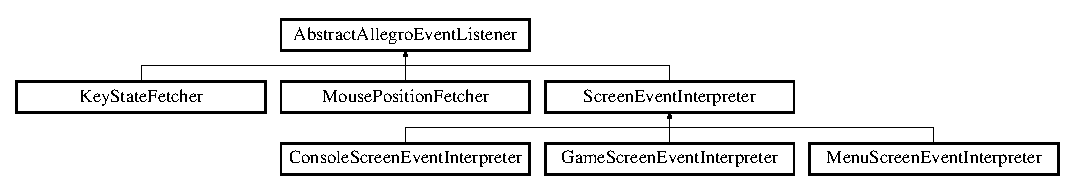
\includegraphics[height=2.121212cm]{classAbstractAllegroEventListener}
\end{center}
\end{figure}
\subsection*{Public Member Functions}
\begin{DoxyCompactItemize}
\item 
virtual void {\bfseries key\+Down} (int keynum)\hypertarget{classAbstractAllegroEventListener_a90feb73dcf27ed7a59a414e0ec9b5dc7}{}\label{classAbstractAllegroEventListener_a90feb73dcf27ed7a59a414e0ec9b5dc7}

\item 
virtual void {\bfseries key\+Up} (int keynum)\hypertarget{classAbstractAllegroEventListener_a184ad8170383d387b1d74dbea49b17fe}{}\label{classAbstractAllegroEventListener_a184ad8170383d387b1d74dbea49b17fe}

\item 
virtual void {\bfseries mouse\+Key\+Down} (int keynum)\hypertarget{classAbstractAllegroEventListener_a0298053859a7fbf0112812472a36d742}{}\label{classAbstractAllegroEventListener_a0298053859a7fbf0112812472a36d742}

\item 
virtual void {\bfseries mouse\+Key\+Up} (int keynum)\hypertarget{classAbstractAllegroEventListener_a6d1c0f830af8870f4453961c491c2fff}{}\label{classAbstractAllegroEventListener_a6d1c0f830af8870f4453961c491c2fff}

\item 
virtual void {\bfseries time\+Event} ()\hypertarget{classAbstractAllegroEventListener_aef255f2df2f0096f6e15ddfac0367e23}{}\label{classAbstractAllegroEventListener_aef255f2df2f0096f6e15ddfac0367e23}

\item 
virtual void {\bfseries char\+Key\+Down} (int unicode)\hypertarget{classAbstractAllegroEventListener_ada1bdbac1038704d3b79b46af1b4221e}{}\label{classAbstractAllegroEventListener_ada1bdbac1038704d3b79b46af1b4221e}

\end{DoxyCompactItemize}


The documentation for this class was generated from the following file\+:\begin{DoxyCompactItemize}
\item 
src/\+Controller/Abstract\+Allegro\+Event\+Listener.\+h\end{DoxyCompactItemize}

\hypertarget{classActor}{}\section{Actor Class Reference}
\label{classActor}\index{Actor@{Actor}}
Inheritance diagram for Actor\+:\begin{figure}[H]
\begin{center}
\leavevmode
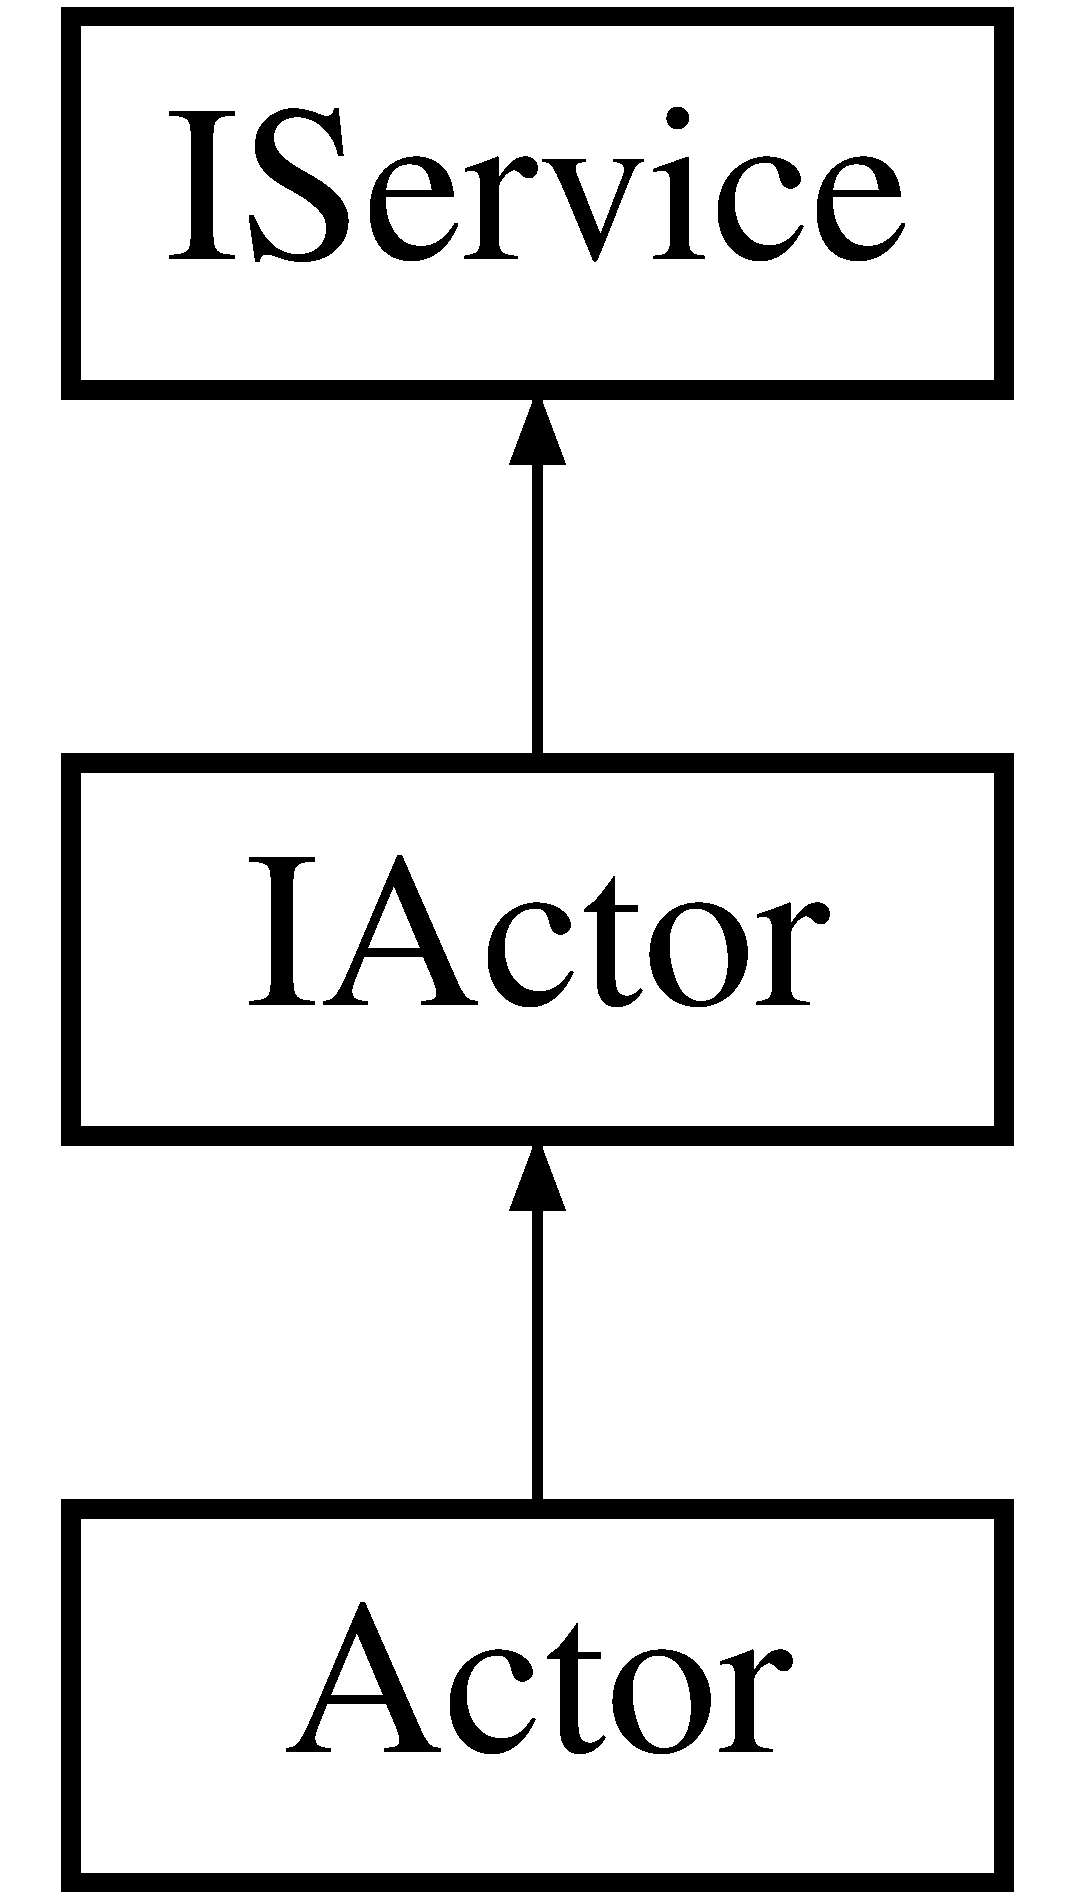
\includegraphics[height=3.000000cm]{classActor}
\end{center}
\end{figure}
\subsection*{Public Member Functions}
\begin{DoxyCompactItemize}
\item 
virtual std\+::shared\+\_\+ptr$<$ \hyperlink{classComponent}{Component} $>$ {\bfseries get\+Only\+Component} (\hyperlink{classComponentTypeChecker}{Component\+Type\+Checker} checker)\hypertarget{classActor_a975ec063e7e6058541057e65a10d7c5b}{}\label{classActor_a975ec063e7e6058541057e65a10d7c5b}

\item 
virtual bool {\bfseries is\+Component\+Present} (\hyperlink{classComponentTypeChecker}{Component\+Type\+Checker} checker)\hypertarget{classActor_a4e94dec1e0c20048e28213e585f875db}{}\label{classActor_a4e94dec1e0c20048e28213e585f875db}

\item 
{\bfseries Actor} (Actor\+Id id)\hypertarget{classActor_a7fea1ceaf2fbd6e08c058fdad2108a06}{}\label{classActor_a7fea1ceaf2fbd6e08c058fdad2108a06}

\item 
virtual void {\bfseries On\+Start} ()\hypertarget{classActor_a926354cddd1e36f1c887144deaa9e9e2}{}\label{classActor_a926354cddd1e36f1c887144deaa9e9e2}

\item 
virtual void {\bfseries On\+Update} ()\hypertarget{classActor_a163d4b04407ff2d748094fca4c472e85}{}\label{classActor_a163d4b04407ff2d748094fca4c472e85}

\item 
virtual void {\bfseries On\+Stop} ()\hypertarget{classActor_a79bbc72a5eeb4eeba06a4ca24da2ef8a}{}\label{classActor_a79bbc72a5eeb4eeba06a4ca24da2ef8a}

\item 
virtual void {\bfseries remove\+Component} (\hyperlink{classComponent}{Component} $\ast$component) override\hypertarget{classActor_ad5b860c18af10e1e27a546100a21ac7b}{}\label{classActor_ad5b860c18af10e1e27a546100a21ac7b}

\item 
virtual void {\bfseries add\+Component} (std\+::shared\+\_\+ptr$<$ \hyperlink{classComponent}{Component} $>$ component) override\hypertarget{classActor_ac1a9cb85ed2193374ecec0e8e1f0778e}{}\label{classActor_ac1a9cb85ed2193374ecec0e8e1f0778e}

\item 
virtual Actor\+Id {\bfseries get\+Actor\+Id} () const \hypertarget{classActor_a28e3c3abb4b2f09027ff2f3805a02895}{}\label{classActor_a28e3c3abb4b2f09027ff2f3805a02895}

\end{DoxyCompactItemize}


The documentation for this class was generated from the following files\+:\begin{DoxyCompactItemize}
\item 
src/\+Model/\+Actors/Actor.\+h\item 
src/\+Model/\+Actors/Actor.\+cpp\end{DoxyCompactItemize}

\hypertarget{classActorIdGenerator}{}\section{Actor\+Id\+Generator Class Reference}
\label{classActorIdGenerator}\index{Actor\+Id\+Generator@{Actor\+Id\+Generator}}
\subsection*{Public Member Functions}
\begin{DoxyCompactItemize}
\item 
Actor\+Id {\bfseries get\+Actor\+Id} ()\hypertarget{classActorIdGenerator_a7076d70292edf2a2a04aaafb8c86415e}{}\label{classActorIdGenerator_a7076d70292edf2a2a04aaafb8c86415e}

\end{DoxyCompactItemize}


The documentation for this class was generated from the following files\+:\begin{DoxyCompactItemize}
\item 
src/\+Model/\+Actors/Actor\+Id\+Generator.\+h\item 
src/\+Model/\+Actors/Actor\+Id\+Generator.\+cpp\end{DoxyCompactItemize}

\hypertarget{classActorOnOutOfScreenDestroyerComponent}{}\section{Actor\+On\+Out\+Of\+Screen\+Destroyer\+Component Class Reference}
\label{classActorOnOutOfScreenDestroyerComponent}\index{Actor\+On\+Out\+Of\+Screen\+Destroyer\+Component@{Actor\+On\+Out\+Of\+Screen\+Destroyer\+Component}}
Inheritance diagram for Actor\+On\+Out\+Of\+Screen\+Destroyer\+Component\+:\begin{figure}[H]
\begin{center}
\leavevmode
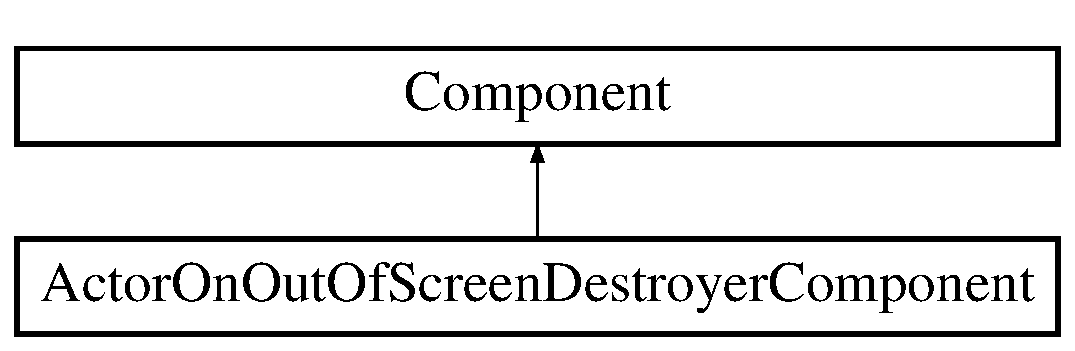
\includegraphics[height=2.000000cm]{classActorOnOutOfScreenDestroyerComponent}
\end{center}
\end{figure}
\subsection*{Public Member Functions}
\begin{DoxyCompactItemize}
\item 
{\bfseries Actor\+On\+Out\+Of\+Screen\+Destroyer\+Component} (\hyperlink{classGameConfiguration}{Game\+Configuration} \&configuration\+\_\+, std\+::shared\+\_\+ptr$<$ \hyperlink{classActorsContainer}{Actors\+Container} $>$ \&actors\+Container\+\_\+)\hypertarget{classActorOnOutOfScreenDestroyerComponent_a70e6a07f9b53acd79f7bdd95f8445a93}{}\label{classActorOnOutOfScreenDestroyerComponent_a70e6a07f9b53acd79f7bdd95f8445a93}

\item 
void {\bfseries On\+Start} (\hyperlink{classIActor}{I\+Actor} \&actor)\hypertarget{classActorOnOutOfScreenDestroyerComponent_ab2c817cc86953214f066464f89e70c37}{}\label{classActorOnOutOfScreenDestroyerComponent_ab2c817cc86953214f066464f89e70c37}

\item 
void {\bfseries On\+Update} ()\hypertarget{classActorOnOutOfScreenDestroyerComponent_a3dac4185cab4e023f3578444f3010a2c}{}\label{classActorOnOutOfScreenDestroyerComponent_a3dac4185cab4e023f3578444f3010a2c}

\end{DoxyCompactItemize}


The documentation for this class was generated from the following files\+:\begin{DoxyCompactItemize}
\item 
src/\+Model/components/Actor\+On\+Out\+Of\+Screen\+Destroyer\+Component.\+h\item 
src/\+Model/components/Actor\+On\+Out\+Of\+Screen\+Destroyer\+Component.\+cpp\end{DoxyCompactItemize}

\hypertarget{classActorsContainer}{}\section{Actors\+Container Class Reference}
\label{classActorsContainer}\index{Actors\+Container@{Actors\+Container}}
Inheritance diagram for Actors\+Container\+:\begin{figure}[H]
\begin{center}
\leavevmode
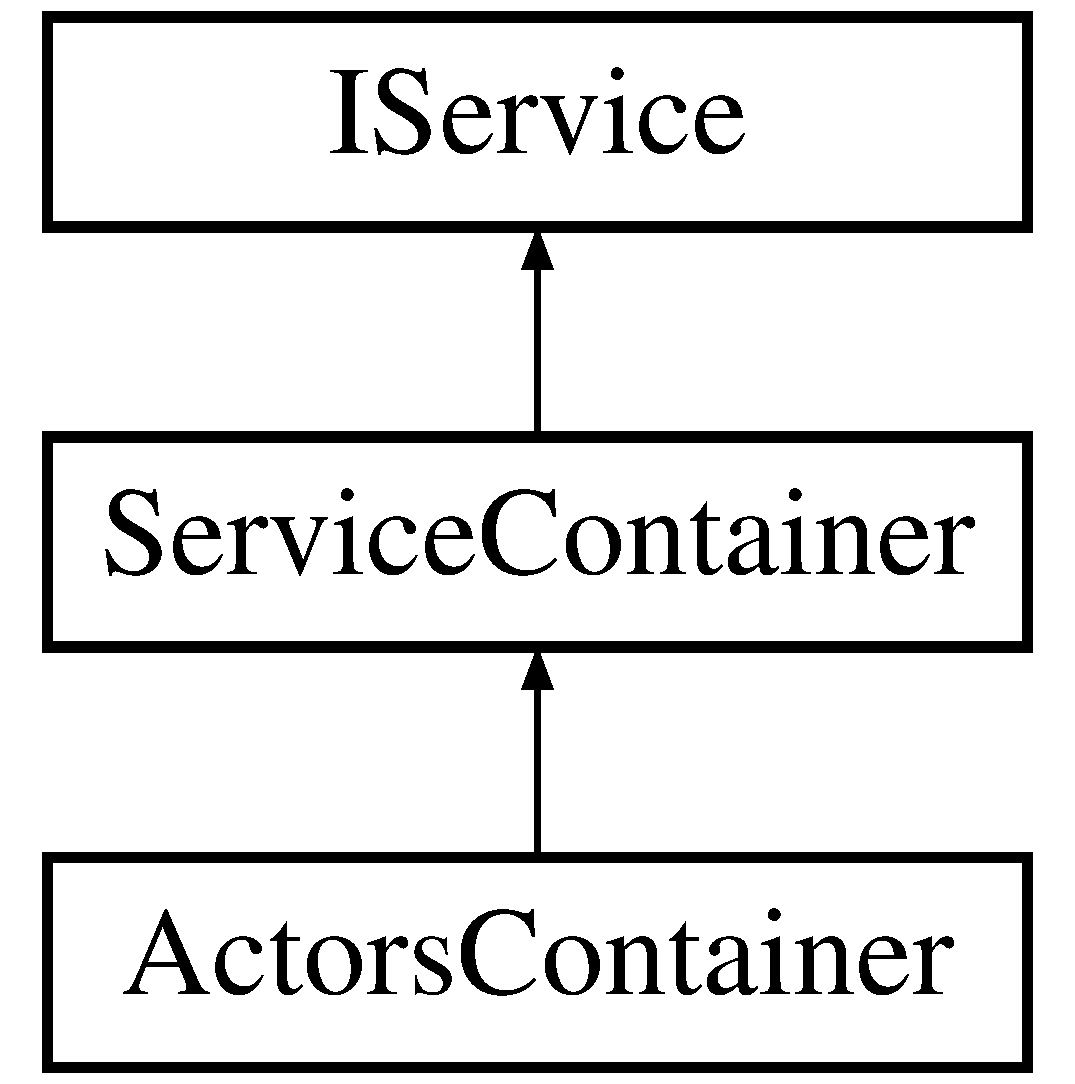
\includegraphics[height=3.000000cm]{classActorsContainer}
\end{center}
\end{figure}
\subsection*{Public Member Functions}
\begin{DoxyCompactItemize}
\item 
{\bfseries Actors\+Container} (\hyperlink{classPythonModule}{Python\+Module} \&python)\hypertarget{classActorsContainer_a1ab15fe14a06a9692ab56284b1626411}{}\label{classActorsContainer_a1ab15fe14a06a9692ab56284b1626411}

\item 
virtual void {\bfseries On\+Start} ()\hypertarget{classActorsContainer_a34beffae5a573714b04971ebc465607d}{}\label{classActorsContainer_a34beffae5a573714b04971ebc465607d}

\item 
std\+::vector$<$ \hyperlink{classPythonActorComponent}{Python\+Actor\+Component} $>$ {\bfseries get\+All\+Actors} ()\hypertarget{classActorsContainer_a31bc1fb0617d8aaa76fc737e4b4a6ae5}{}\label{classActorsContainer_a31bc1fb0617d8aaa76fc737e4b4a6ae5}

\item 
void {\bfseries add\+Actor} (std\+::shared\+\_\+ptr$<$ \hyperlink{classIActor}{I\+Actor} $>$ new\+Actor)\hypertarget{classActorsContainer_a1e95e6ee2558da4e7bb14c889a0d416b}{}\label{classActorsContainer_a1e95e6ee2558da4e7bb14c889a0d416b}

\item 
void {\bfseries add\+Actor\+During\+Runtime} (std\+::shared\+\_\+ptr$<$ \hyperlink{classIActor}{I\+Actor} $>$ new\+Actor)\hypertarget{classActorsContainer_aeb74636b92532dbfcf674e6d98ff76b8}{}\label{classActorsContainer_aeb74636b92532dbfcf674e6d98ff76b8}

\item 
void {\bfseries remove\+Actor} (std\+::shared\+\_\+ptr$<$ \hyperlink{classIActor}{I\+Actor} $>$ new\+Actor)\hypertarget{classActorsContainer_a0f4efa35b84767e3156c8e6affc139e3}{}\label{classActorsContainer_a0f4efa35b84767e3156c8e6affc139e3}

\item 
void {\bfseries remove\+Actor} (\hyperlink{classPythonActorComponent}{Python\+Actor\+Component} \&python\+Actor\+Component)\hypertarget{classActorsContainer_a572b8b7a645027fc6c2a3c8a2d92bd03}{}\label{classActorsContainer_a572b8b7a645027fc6c2a3c8a2d92bd03}

\item 
void {\bfseries remove\+Actor\+By\+Id} (Actor\+Id id)\hypertarget{classActorsContainer_a261fed6fb7490153d42dc9a1675d6f85}{}\label{classActorsContainer_a261fed6fb7490153d42dc9a1675d6f85}

\item 
void {\bfseries reset\+And\+Remove\+All\+Actors} ()\hypertarget{classActorsContainer_ab61682f3c61e766c93f3bbe77436008b}{}\label{classActorsContainer_ab61682f3c61e766c93f3bbe77436008b}

\end{DoxyCompactItemize}
\subsection*{Protected Member Functions}
\begin{DoxyCompactItemize}
\item 
virtual std\+::vector$<$ std\+::shared\+\_\+ptr$<$ \hyperlink{classIService}{I\+Service} $>$ $>$ {\bfseries get\+Services} ()\hypertarget{classActorsContainer_a13b62950aa6b619061b0b3e120d4811a}{}\label{classActorsContainer_a13b62950aa6b619061b0b3e120d4811a}

\end{DoxyCompactItemize}


The documentation for this class was generated from the following files\+:\begin{DoxyCompactItemize}
\item 
src/\+Model/\+Services/Actors\+Container.\+h\item 
src/\+Model/\+Services/Actors\+Container.\+cpp\end{DoxyCompactItemize}

\hypertarget{classActorsContainerTest}{}\section{Actors\+Container\+Test Class Reference}
\label{classActorsContainerTest}\index{Actors\+Container\+Test@{Actors\+Container\+Test}}
Inheritance diagram for Actors\+Container\+Test\+:\begin{figure}[H]
\begin{center}
\leavevmode
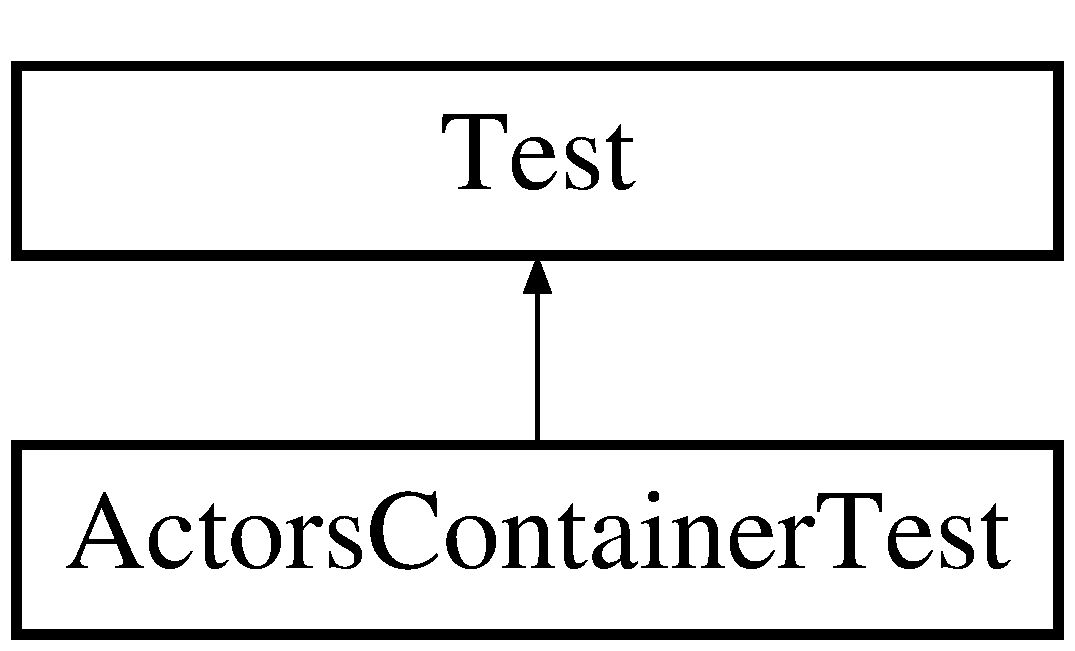
\includegraphics[height=2.000000cm]{classActorsContainerTest}
\end{center}
\end{figure}
\subsection*{Public Member Functions}
\begin{DoxyCompactItemize}
\item 
std\+::vector$<$ std\+::shared\+\_\+ptr$<$ \hyperlink{classIActor}{I\+Actor} $>$ $>$ {\bfseries get\+Actors\+Vec} ()\hypertarget{classActorsContainerTest_a62bd5be2db86065af7ec583b2605475e}{}\label{classActorsContainerTest_a62bd5be2db86065af7ec583b2605475e}

\end{DoxyCompactItemize}
\subsection*{Public Attributes}
\begin{DoxyCompactItemize}
\item 
\hyperlink{classPythonModule}{Python\+Module} {\bfseries mock\+Python}\hypertarget{classActorsContainerTest_aa5fcefa886f5955c2a3461fbf08cba4e}{}\label{classActorsContainerTest_aa5fcefa886f5955c2a3461fbf08cba4e}

\end{DoxyCompactItemize}


The documentation for this class was generated from the following file\+:\begin{DoxyCompactItemize}
\item 
test/\+Services/Actors\+Container\+Test.\+cpp\end{DoxyCompactItemize}

\hypertarget{classActorsGenerator}{}\section{Actors\+Generator Class Reference}
\label{classActorsGenerator}\index{Actors\+Generator@{Actors\+Generator}}
Inheritance diagram for Actors\+Generator\+:\begin{figure}[H]
\begin{center}
\leavevmode
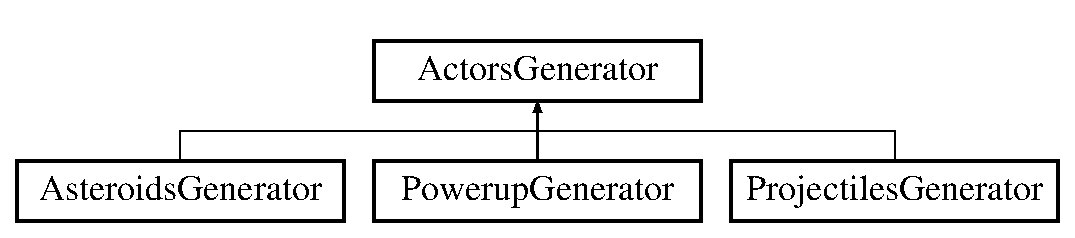
\includegraphics[height=2.000000cm]{classActorsGenerator}
\end{center}
\end{figure}
\subsection*{Protected Member Functions}
\begin{DoxyCompactItemize}
\item 
{\bfseries Actors\+Generator} (std\+::shared\+\_\+ptr$<$ \hyperlink{classActorsContainer}{Actors\+Container} $>$ actors\+Container\+\_\+, \hyperlink{classActorIdGenerator}{Actor\+Id\+Generator} \&id\+Generator\+\_\+, \hyperlink{classPythonModule}{Python\+Module} \&python\+Module\+\_\+, \hyperlink{classDrawingSystem}{Drawing\+System} \&drawing\+System\+\_\+, \hyperlink{classGameConfiguration}{Game\+Configuration} \&game\+Configuration\+\_\+, std\+::shared\+\_\+ptr$<$ \hyperlink{classBox2DService}{Box2\+D\+Service} $>$ box\+Service\+\_\+, \hyperlink{classBox2dObjectsContainer}{Box2d\+Objects\+Container} \&container\+\_\+, \hyperlink{classImageScalesContainer}{Image\+Scales\+Container} \&image\+Scales\+Container, \hyperlink{classContactComponentsContainer}{Contact\+Components\+Container} \&contact\+Components\+Container)\hypertarget{classActorsGenerator_aab32aafd3494be1c40a13e13b0e192ae}{}\label{classActorsGenerator_aab32aafd3494be1c40a13e13b0e192ae}

\item 
void {\bfseries generate\+Actor} (std\+::vector$<$ std\+::shared\+\_\+ptr$<$ \hyperlink{classComponent}{Component} $>$$>$ components\+Vector, \hyperlink{classPoint}{Point} position, \hyperlink{classRotation}{Rotation} rotation, \hyperlink{classPoint}{Point} speed\+Vector, double rotation\+Speed)\hypertarget{classActorsGenerator_a2c45dd6a3d9620c9544eff75a7c8aed1}{}\label{classActorsGenerator_a2c45dd6a3d9620c9544eff75a7c8aed1}

\end{DoxyCompactItemize}
\subsection*{Protected Attributes}
\begin{DoxyCompactItemize}
\item 
std\+::shared\+\_\+ptr$<$ \hyperlink{classActorsContainer}{Actors\+Container} $>$ {\bfseries actors\+Container\+\_\+}\hypertarget{classActorsGenerator_aed600418e9fea552613186e17f29b125}{}\label{classActorsGenerator_aed600418e9fea552613186e17f29b125}

\item 
\hyperlink{classActorIdGenerator}{Actor\+Id\+Generator} \& {\bfseries id\+Generator\+\_\+}\hypertarget{classActorsGenerator_a9ba70a27e3f86fe57fcdf6d46f3a458e}{}\label{classActorsGenerator_a9ba70a27e3f86fe57fcdf6d46f3a458e}

\item 
\hyperlink{classPythonModule}{Python\+Module} \& {\bfseries python\+Module\+\_\+}\hypertarget{classActorsGenerator_ad5b9bb4d9a81ee9c3b0120665e87feb9}{}\label{classActorsGenerator_ad5b9bb4d9a81ee9c3b0120665e87feb9}

\item 
\hyperlink{classDrawingSystem}{Drawing\+System} \& {\bfseries drawing\+System\+\_\+}\hypertarget{classActorsGenerator_ab411f397987566303f657d4d6c3eddad}{}\label{classActorsGenerator_ab411f397987566303f657d4d6c3eddad}

\item 
\hyperlink{classGameConfiguration}{Game\+Configuration} \& {\bfseries game\+Configuration\+\_\+}\hypertarget{classActorsGenerator_a142b3da2ed4c32b042892560f7cfadf2}{}\label{classActorsGenerator_a142b3da2ed4c32b042892560f7cfadf2}

\item 
std\+::shared\+\_\+ptr$<$ \hyperlink{classBox2DService}{Box2\+D\+Service} $>$ {\bfseries box\+Service\+\_\+}\hypertarget{classActorsGenerator_ac14a3f51f8c6eb95a529416cc49c254b}{}\label{classActorsGenerator_ac14a3f51f8c6eb95a529416cc49c254b}

\item 
\hyperlink{classBox2dObjectsContainer}{Box2d\+Objects\+Container} \& {\bfseries container\+\_\+}\hypertarget{classActorsGenerator_ab75d25e9aa597a0e944884a7dc65741c}{}\label{classActorsGenerator_ab75d25e9aa597a0e944884a7dc65741c}

\item 
\hyperlink{classImageScalesContainer}{Image\+Scales\+Container} \& {\bfseries image\+Scales\+Container\+\_\+}\hypertarget{classActorsGenerator_ab115e37c12f48588ddb0e1328ecd028e}{}\label{classActorsGenerator_ab115e37c12f48588ddb0e1328ecd028e}

\item 
\hyperlink{classContactComponentsContainer}{Contact\+Components\+Container} \& {\bfseries contact\+Components\+Container\+\_\+}\hypertarget{classActorsGenerator_ad80c8ccabe2be13b681e1116635aa387}{}\label{classActorsGenerator_ad80c8ccabe2be13b681e1116635aa387}

\end{DoxyCompactItemize}


The documentation for this class was generated from the following files\+:\begin{DoxyCompactItemize}
\item 
src/\+Model/\+Actors/Actors\+Generator.\+h\item 
src/\+Model/\+Actors/Actors\+Generator.\+cpp\end{DoxyCompactItemize}

\hypertarget{classActorTests}{}\section{Actor\+Tests Class Reference}
\label{classActorTests}\index{Actor\+Tests@{Actor\+Tests}}
Inheritance diagram for Actor\+Tests\+:\begin{figure}[H]
\begin{center}
\leavevmode
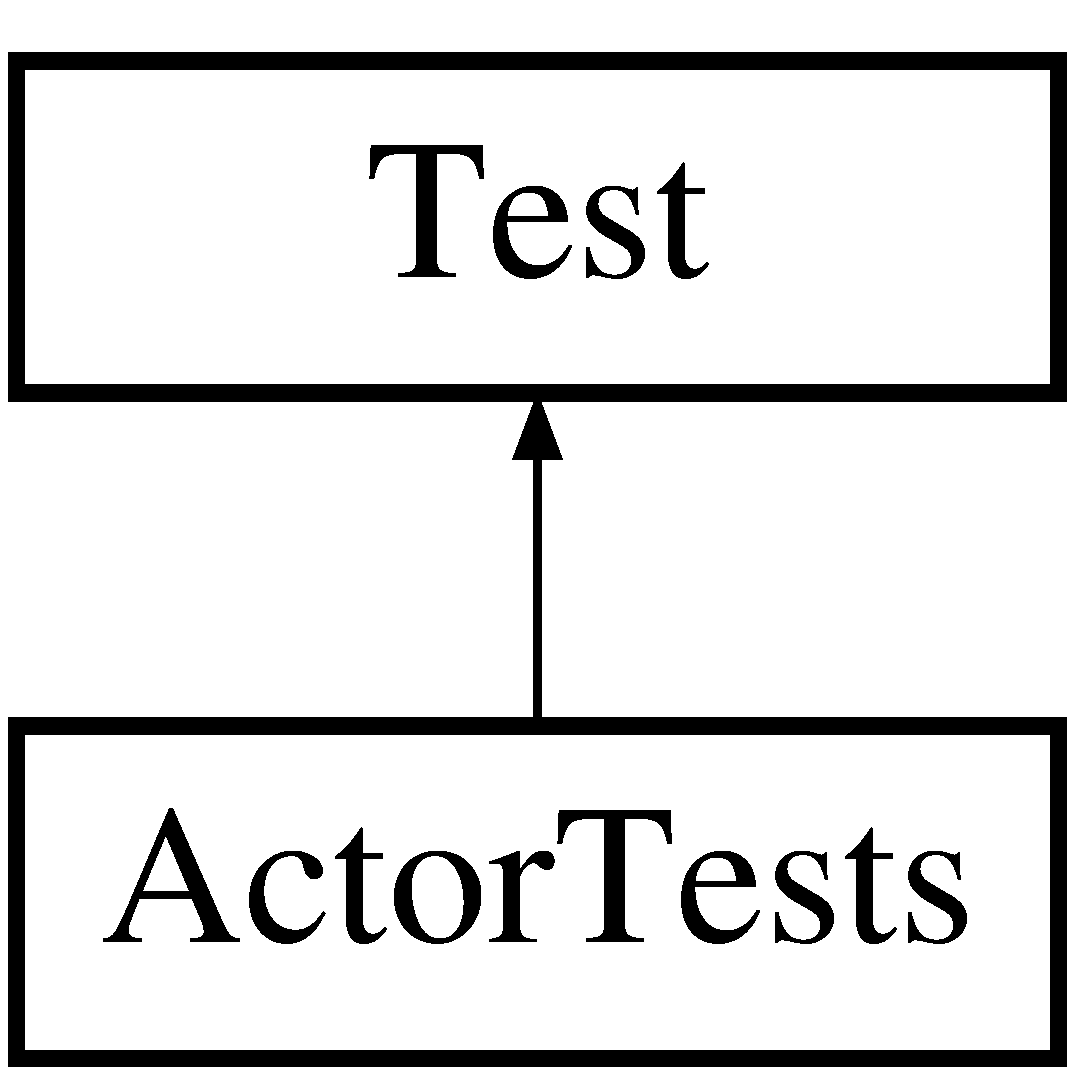
\includegraphics[height=2.000000cm]{classActorTests}
\end{center}
\end{figure}
\subsection*{Public Member Functions}
\begin{DoxyCompactItemize}
\item 
std\+::vector$<$ std\+::shared\+\_\+ptr$<$ \hyperlink{classMockComponent}{Mock\+Component} $>$ $>$ {\bfseries create\+Strict\+Mock\+Components\+Vector} ()\hypertarget{classActorTests_a020b0bc3c5d4d21df25d5a2e26bc7cde}{}\label{classActorTests_a020b0bc3c5d4d21df25d5a2e26bc7cde}

\item 
std\+::vector$<$ std\+::shared\+\_\+ptr$<$ \hyperlink{classMockComponent}{Mock\+Component} $>$ $>$ {\bfseries create\+Mock\+Components\+Vector} ()\hypertarget{classActorTests_a7c3f25ceee44a4e1afd8b9a679c90e89}{}\label{classActorTests_a7c3f25ceee44a4e1afd8b9a679c90e89}

\item 
void {\bfseries add\+Components\+To\+Actor} (std\+::vector$<$ std\+::shared\+\_\+ptr$<$ \hyperlink{classMockComponent}{Mock\+Component} $>$$>$ in\+Vec)\hypertarget{classActorTests_a6faea7f33a95d348a683991b15af6fd3}{}\label{classActorTests_a6faea7f33a95d348a683991b15af6fd3}

\end{DoxyCompactItemize}
\subsection*{Public Attributes}
\begin{DoxyCompactItemize}
\item 
\hyperlink{classActor}{Actor} {\bfseries actor}\hypertarget{classActorTests_a85f068f735c773909d7779407b3db165}{}\label{classActorTests_a85f068f735c773909d7779407b3db165}

\end{DoxyCompactItemize}


The documentation for this class was generated from the following file\+:\begin{DoxyCompactItemize}
\item 
test/Actor\+Test.\+cpp\end{DoxyCompactItemize}

\hypertarget{classActorTypeComponent}{}\section{Actor\+Type\+Component Class Reference}
\label{classActorTypeComponent}\index{Actor\+Type\+Component@{Actor\+Type\+Component}}
Inheritance diagram for Actor\+Type\+Component\+:\begin{figure}[H]
\begin{center}
\leavevmode
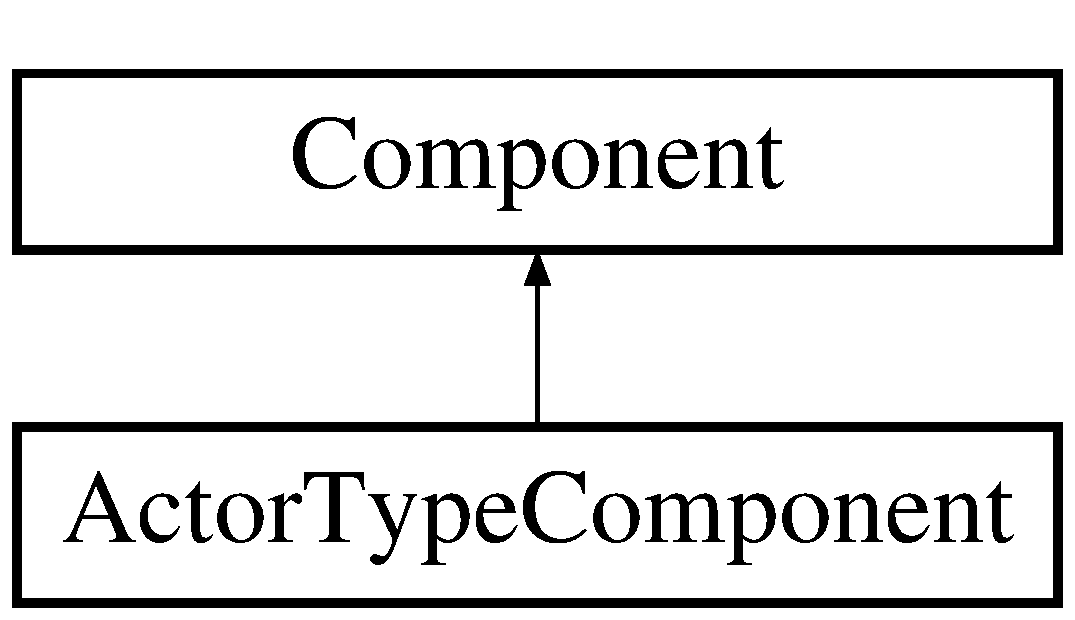
\includegraphics[height=2.000000cm]{classActorTypeComponent}
\end{center}
\end{figure}
\subsection*{Public Member Functions}
\begin{DoxyCompactItemize}
\item 
{\bfseries Actor\+Type\+Component} (Actor\+Type type, \hyperlink{classPythonModule}{Python\+Module} \&python\+Module)\hypertarget{classActorTypeComponent_ad7501c6cbcb34fb5152f40ba3914a1b9}{}\label{classActorTypeComponent_ad7501c6cbcb34fb5152f40ba3914a1b9}

\item 
virtual void {\bfseries On\+Start} (\hyperlink{classIActor}{I\+Actor} \&actor)\hypertarget{classActorTypeComponent_a04af8d4297a9aeb340af3af95ca0ed1e}{}\label{classActorTypeComponent_a04af8d4297a9aeb340af3af95ca0ed1e}

\item 
std\+::string {\bfseries get\+Actor\+Type} ()\hypertarget{classActorTypeComponent_a55143b2857baa0dfe7875d7c0a2271ca}{}\label{classActorTypeComponent_a55143b2857baa0dfe7875d7c0a2271ca}

\end{DoxyCompactItemize}


The documentation for this class was generated from the following files\+:\begin{DoxyCompactItemize}
\item 
src/\+Model/components/Actor\+Type\+Component.\+h\item 
src/\+Model/components/Actor\+Type\+Component.\+cpp\end{DoxyCompactItemize}

\hypertarget{classAllegroEventInterpreter}{}\section{Allegro\+Event\+Interpreter Class Reference}
\label{classAllegroEventInterpreter}\index{Allegro\+Event\+Interpreter@{Allegro\+Event\+Interpreter}}
\subsection*{Public Member Functions}
\begin{DoxyCompactItemize}
\item 
void {\bfseries interpret\+Event} (A\+L\+L\+E\+G\+R\+O\+\_\+\+E\+V\+E\+NT event)\hypertarget{classAllegroEventInterpreter_a572641b277345083016ce9920fcc8d33}{}\label{classAllegroEventInterpreter_a572641b277345083016ce9920fcc8d33}

\item 
void {\bfseries add\+Listener} (\hyperlink{classAbstractAllegroEventListener}{Abstract\+Allegro\+Event\+Listener} $\ast$listener)\hypertarget{classAllegroEventInterpreter_acf06da41e2c92011bacfe6c6775cc1ee}{}\label{classAllegroEventInterpreter_acf06da41e2c92011bacfe6c6775cc1ee}

\item 
void {\bfseries remove\+Listener} (\hyperlink{classScreenEventInterpreter}{Screen\+Event\+Interpreter} $\ast$interpreter)\hypertarget{classAllegroEventInterpreter_a44f231d861c8d523298c3143bbd7749d}{}\label{classAllegroEventInterpreter_a44f231d861c8d523298c3143bbd7749d}

\end{DoxyCompactItemize}


The documentation for this class was generated from the following files\+:\begin{DoxyCompactItemize}
\item 
src/\+Controller/Allegro\+Event\+Interpreter.\+h\item 
src/\+Controller/Allegro\+Event\+Interpreter.\+cpp\end{DoxyCompactItemize}

\hypertarget{classAllegroToGameKeyMapper}{}\section{Allegro\+To\+Game\+Key\+Mapper Class Reference}
\label{classAllegroToGameKeyMapper}\index{Allegro\+To\+Game\+Key\+Mapper@{Allegro\+To\+Game\+Key\+Mapper}}
\subsection*{Public Member Functions}
\begin{DoxyCompactItemize}
\item 
{\bfseries Allegro\+To\+Game\+Key\+Mapper} (\hyperlink{classKeyStateFetcher}{Key\+State\+Fetcher} \&key\+State\+Fetcher, std\+::map$<$ int, Keys $>$ keyboard\+To\+Game\+Key\+Map, std\+::map$<$ int, Keys $>$ mouse\+To\+Game\+Key\+Map)\hypertarget{classAllegroToGameKeyMapper_a8d316653102f98411984ab2b4b4c6f70}{}\label{classAllegroToGameKeyMapper_a8d316653102f98411984ab2b4b4c6f70}

\item 
std\+::vector$<$ Keys $>$ {\bfseries get\+Pressed\+Keys} ()\hypertarget{classAllegroToGameKeyMapper_a88d81b6ac9b28fbc8df7ea0b3de1e3f2}{}\label{classAllegroToGameKeyMapper_a88d81b6ac9b28fbc8df7ea0b3de1e3f2}

\end{DoxyCompactItemize}


The documentation for this class was generated from the following files\+:\begin{DoxyCompactItemize}
\item 
src/\+Controller/Allegro\+To\+Game\+Key\+Mapper.\+h\item 
src/\+Controller/Allegro\+To\+Game\+Key\+Mapper.\+cpp\end{DoxyCompactItemize}

\hypertarget{classAsteroidCollisionComponent}{}\section{Asteroid\+Collision\+Component Class Reference}
\label{classAsteroidCollisionComponent}\index{Asteroid\+Collision\+Component@{Asteroid\+Collision\+Component}}
Inheritance diagram for Asteroid\+Collision\+Component\+:\begin{figure}[H]
\begin{center}
\leavevmode
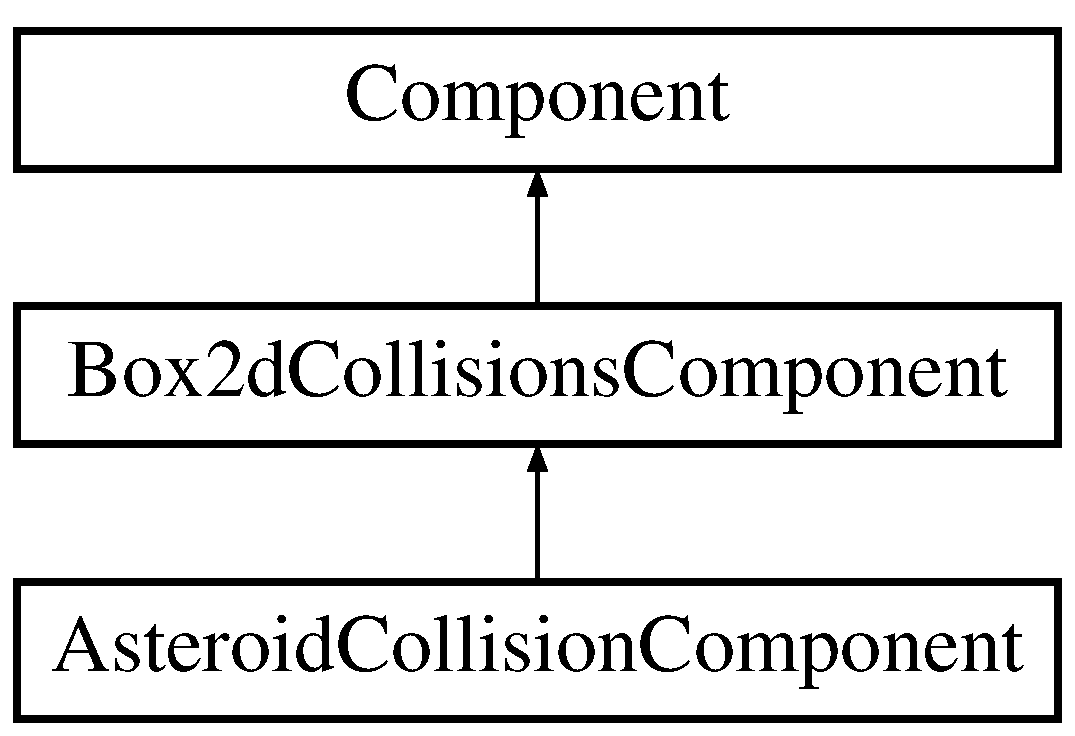
\includegraphics[height=3.000000cm]{classAsteroidCollisionComponent}
\end{center}
\end{figure}
\subsection*{Public Member Functions}
\begin{DoxyCompactItemize}
\item 
{\bfseries Asteroid\+Collision\+Component} (\hyperlink{classContactComponentsContainer}{Contact\+Components\+Container} \&contact\+Container, std\+::shared\+\_\+ptr$<$ \hyperlink{classActorsContainer}{Actors\+Container} $>$ actors\+Container, \hyperlink{classAsteroidsGenerator}{Asteroids\+Generator} \&asteroids\+Generator, std\+::shared\+\_\+ptr$<$ \hyperlink{classMusicManager}{Music\+Manager} $>$ music\+Manager, \hyperlink{classExplosionCloudGenerator}{Explosion\+Cloud\+Generator} \&cloud\+Generator)\hypertarget{classAsteroidCollisionComponent_a9860abce070e21404cdce554cccb11c3}{}\label{classAsteroidCollisionComponent_a9860abce070e21404cdce554cccb11c3}

\item 
void {\bfseries On\+Start} (\hyperlink{classIActor}{I\+Actor} \&actor)\hypertarget{classAsteroidCollisionComponent_a49bdf342f29806ea409cffedb5634bfb}{}\label{classAsteroidCollisionComponent_a49bdf342f29806ea409cffedb5634bfb}

\item 
bool {\bfseries manage\+Collision} (\hyperlink{structCollisionData}{Collision\+Data} \&data) override\hypertarget{classAsteroidCollisionComponent_a5fb79649b4cb8c0f30a9f52960167ede}{}\label{classAsteroidCollisionComponent_a5fb79649b4cb8c0f30a9f52960167ede}

\item 
void {\bfseries create\+Asteroid\+At\+Angle\+Relative\+To\+Current\+Asteroid} (double impulse\+Value, \hyperlink{classRotation}{Rotation} angle, int asteroid\+Franctions)\hypertarget{classAsteroidCollisionComponent_a61f138ea05e94d9b3738b8b044d1905f}{}\label{classAsteroidCollisionComponent_a61f138ea05e94d9b3738b8b044d1905f}

\end{DoxyCompactItemize}
\subsection*{Additional Inherited Members}


The documentation for this class was generated from the following files\+:\begin{DoxyCompactItemize}
\item 
src/\+Model/\+Actors/\+Asteroid/Asteroid\+Collision\+Component.\+h\item 
src/\+Model/\+Actors/\+Asteroid/Asteroid\+Collision\+Component.\+cpp\end{DoxyCompactItemize}

\hypertarget{classAsteroidCollisionEndToEndTests}{}\section{Asteroid\+Collision\+End\+To\+End\+Tests Class Reference}
\label{classAsteroidCollisionEndToEndTests}\index{Asteroid\+Collision\+End\+To\+End\+Tests@{Asteroid\+Collision\+End\+To\+End\+Tests}}


The documentation for this class was generated from the following file\+:\begin{DoxyCompactItemize}
\item 
test/\+End\+To\+End\+Tests/Asteroid\+Collision\+End\+To\+End\+Tests.\+h\end{DoxyCompactItemize}

\hypertarget{classAsteroidsCounter}{}\section{Asteroids\+Counter Class Reference}
\label{classAsteroidsCounter}\index{Asteroids\+Counter@{Asteroids\+Counter}}
\subsection*{Public Member Functions}
\begin{DoxyCompactItemize}
\item 
void {\bfseries Increment} ()\hypertarget{classAsteroidsCounter_a5bfafaf855f6ddec948db0839a559933}{}\label{classAsteroidsCounter_a5bfafaf855f6ddec948db0839a559933}

\item 
void {\bfseries Decrement} ()\hypertarget{classAsteroidsCounter_a613c1e39f92e674e3e854378375fe77f}{}\label{classAsteroidsCounter_a613c1e39f92e674e3e854378375fe77f}

\item 
int {\bfseries get\+Value} ()\hypertarget{classAsteroidsCounter_a0ae133ae9c11f0dfef444df8f926cdaa}{}\label{classAsteroidsCounter_a0ae133ae9c11f0dfef444df8f926cdaa}

\end{DoxyCompactItemize}


The documentation for this class was generated from the following files\+:\begin{DoxyCompactItemize}
\item 
src/\+Model/\+Actors/\+Asteroid/Asteroids\+Counter.\+h\item 
src/\+Model/\+Actors/\+Asteroid/Asteroids\+Counter.\+cpp\end{DoxyCompactItemize}

\hypertarget{classAsteroidsCountingComponent}{}\section{Asteroids\+Counting\+Component Class Reference}
\label{classAsteroidsCountingComponent}\index{Asteroids\+Counting\+Component@{Asteroids\+Counting\+Component}}
Inheritance diagram for Asteroids\+Counting\+Component\+:\begin{figure}[H]
\begin{center}
\leavevmode
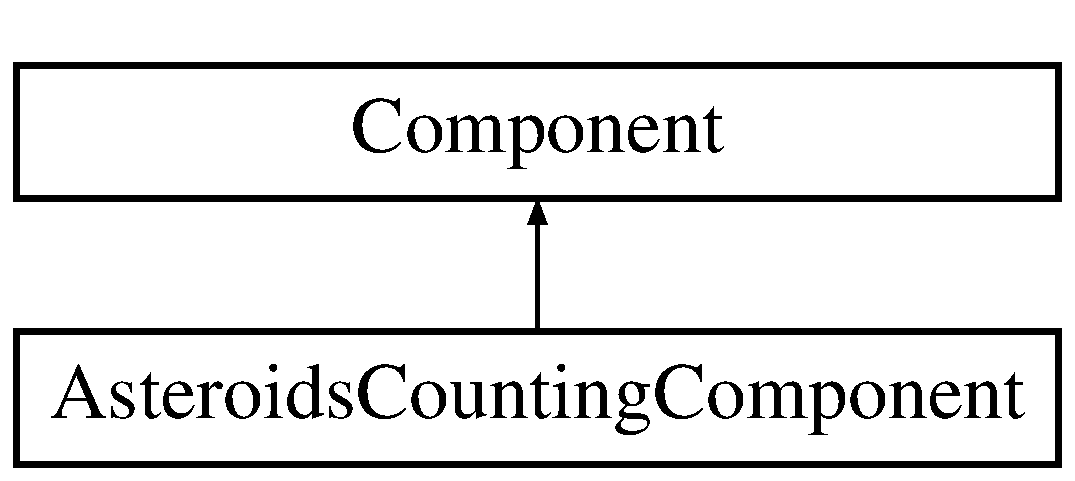
\includegraphics[height=2.000000cm]{classAsteroidsCountingComponent}
\end{center}
\end{figure}
\subsection*{Public Member Functions}
\begin{DoxyCompactItemize}
\item 
{\bfseries Asteroids\+Counting\+Component} (\hyperlink{classAsteroidsCounter}{Asteroids\+Counter} \&counter)\hypertarget{classAsteroidsCountingComponent_aad10e1a5d7b29532820776f9926ce06a}{}\label{classAsteroidsCountingComponent_aad10e1a5d7b29532820776f9926ce06a}

\item 
void {\bfseries On\+Start} (\hyperlink{classIActor}{I\+Actor} \&actor)\hypertarget{classAsteroidsCountingComponent_a47c91c7b22a9223f39c065e615d41dda}{}\label{classAsteroidsCountingComponent_a47c91c7b22a9223f39c065e615d41dda}

\item 
void {\bfseries On\+Stop} ()\hypertarget{classAsteroidsCountingComponent_a08b48b1f45fa415be8148dbc515f0248}{}\label{classAsteroidsCountingComponent_a08b48b1f45fa415be8148dbc515f0248}

\end{DoxyCompactItemize}


The documentation for this class was generated from the following files\+:\begin{DoxyCompactItemize}
\item 
src/\+Model/\+Actors/\+Asteroid/Asteroids\+Counting\+Component.\+h\item 
src/\+Model/\+Actors/\+Asteroid/Asteroids\+Counting\+Component.\+cpp\end{DoxyCompactItemize}

\hypertarget{classAsteroidsGenerator}{}\section{Asteroids\+Generator Class Reference}
\label{classAsteroidsGenerator}\index{Asteroids\+Generator@{Asteroids\+Generator}}
Inheritance diagram for Asteroids\+Generator\+:\begin{figure}[H]
\begin{center}
\leavevmode
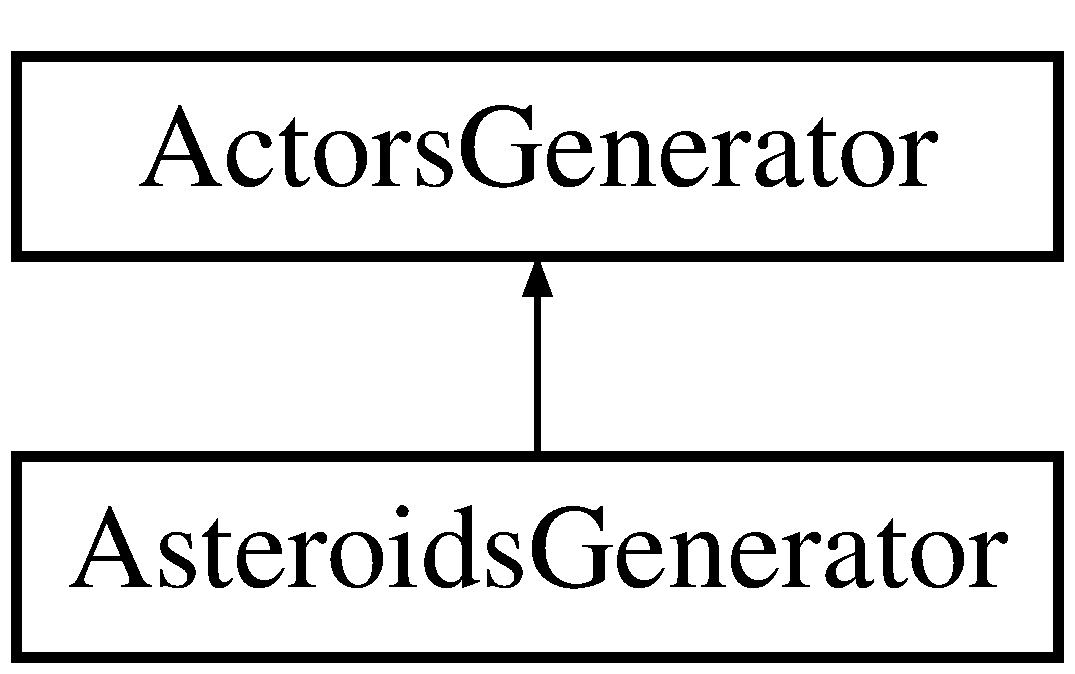
\includegraphics[height=2.000000cm]{classAsteroidsGenerator}
\end{center}
\end{figure}
\subsection*{Public Member Functions}
\begin{DoxyCompactItemize}
\item 
{\bfseries Asteroids\+Generator} (std\+::shared\+\_\+ptr$<$ \hyperlink{classActorsContainer}{Actors\+Container} $>$ actors\+Container, \hyperlink{classActorIdGenerator}{Actor\+Id\+Generator} \&id\+Generator, \hyperlink{classPythonModule}{Python\+Module} \&python\+Module, \hyperlink{classDrawingSystem}{Drawing\+System} \&drawing\+System, \hyperlink{classGameConfiguration}{Game\+Configuration} \&game\+Configuration, std\+::shared\+\_\+ptr$<$ \hyperlink{classBox2DService}{Box2\+D\+Service} $>$ box\+Service, \hyperlink{classBox2dObjectsContainer}{Box2d\+Objects\+Container} \&container, \hyperlink{classImageScalesContainer}{Image\+Scales\+Container} \&image\+Scales\+Container, \hyperlink{classContactComponentsContainer}{Contact\+Components\+Container} \&contact\+Components\+Container, \hyperlink{classAsteroidsCounter}{Asteroids\+Counter} \&asteroids\+Counter, std\+::shared\+\_\+ptr$<$ \hyperlink{classMusicManager}{Music\+Manager} $>$ music\+Manager, \hyperlink{classExplosionCloudGenerator}{Explosion\+Cloud\+Generator} \&cloud\+Generator)\hypertarget{classAsteroidsGenerator_a3fbe934be6652634dde564434e8fe169}{}\label{classAsteroidsGenerator_a3fbe934be6652634dde564434e8fe169}

\item 
void {\bfseries generate\+Asteroid} (\hyperlink{classPoint}{Point} position, \hyperlink{classRotation}{Rotation} rotation, double size, \hyperlink{classPoint}{Point} speed\+Vector, double rotation\+Speed)\hypertarget{classAsteroidsGenerator_a5268e6b8f8ea250427cf6832116c9aa0}{}\label{classAsteroidsGenerator_a5268e6b8f8ea250427cf6832116c9aa0}

\end{DoxyCompactItemize}
\subsection*{Additional Inherited Members}


The documentation for this class was generated from the following files\+:\begin{DoxyCompactItemize}
\item 
src/\+Model/\+Actors/\+Asteroid/Asteroids\+Generator.\+h\item 
src/\+Model/\+Actors/\+Asteroid/Asteroids\+Generator.\+cpp\end{DoxyCompactItemize}

\hypertarget{classAsteroidSizeComponent}{}\section{Asteroid\+Size\+Component Class Reference}
\label{classAsteroidSizeComponent}\index{Asteroid\+Size\+Component@{Asteroid\+Size\+Component}}
Inheritance diagram for Asteroid\+Size\+Component\+:\begin{figure}[H]
\begin{center}
\leavevmode
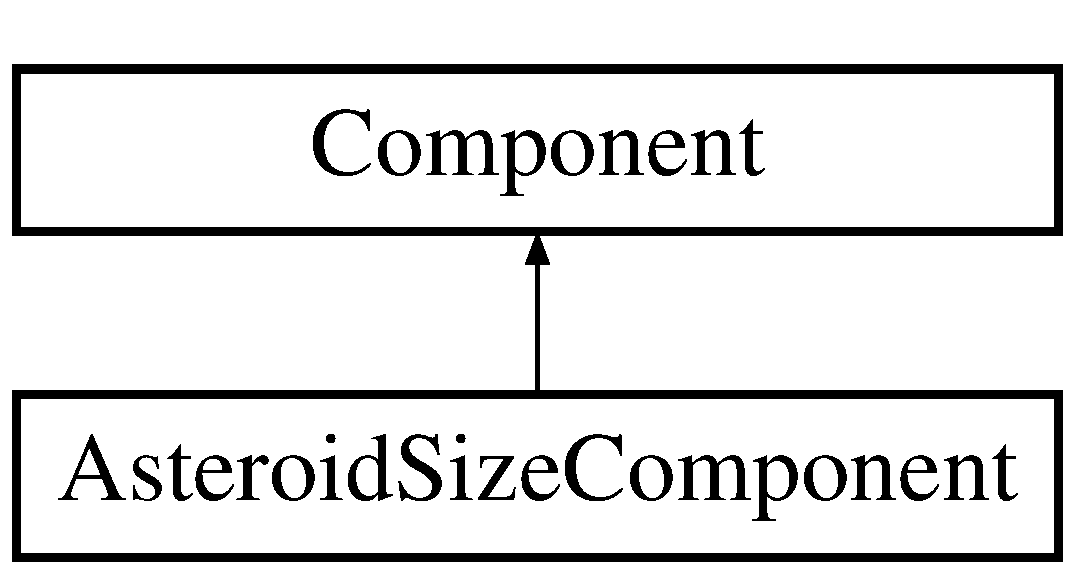
\includegraphics[height=2.000000cm]{classAsteroidSizeComponent}
\end{center}
\end{figure}
\subsection*{Public Member Functions}
\begin{DoxyCompactItemize}
\item 
{\bfseries Asteroid\+Size\+Component} (double size)\hypertarget{classAsteroidSizeComponent_a75c6bbd15b0aac22e48d5bda8ecaba22}{}\label{classAsteroidSizeComponent_a75c6bbd15b0aac22e48d5bda8ecaba22}

\item 
double {\bfseries get\+Size} ()\hypertarget{classAsteroidSizeComponent_a02117cd143700e333623eb0e25dfea32}{}\label{classAsteroidSizeComponent_a02117cd143700e333623eb0e25dfea32}

\end{DoxyCompactItemize}


The documentation for this class was generated from the following files\+:\begin{DoxyCompactItemize}
\item 
src/\+Model/\+Actors/\+Asteroid/Asteroid\+Size\+Component.\+h\item 
src/\+Model/\+Actors/\+Asteroid/Asteroid\+Size\+Component.\+cpp\end{DoxyCompactItemize}

\hypertarget{classAsteroidsTest}{}\section{Asteroids\+Test Class Reference}
\label{classAsteroidsTest}\index{Asteroids\+Test@{Asteroids\+Test}}
Inheritance diagram for Asteroids\+Test\+:\begin{figure}[H]
\begin{center}
\leavevmode
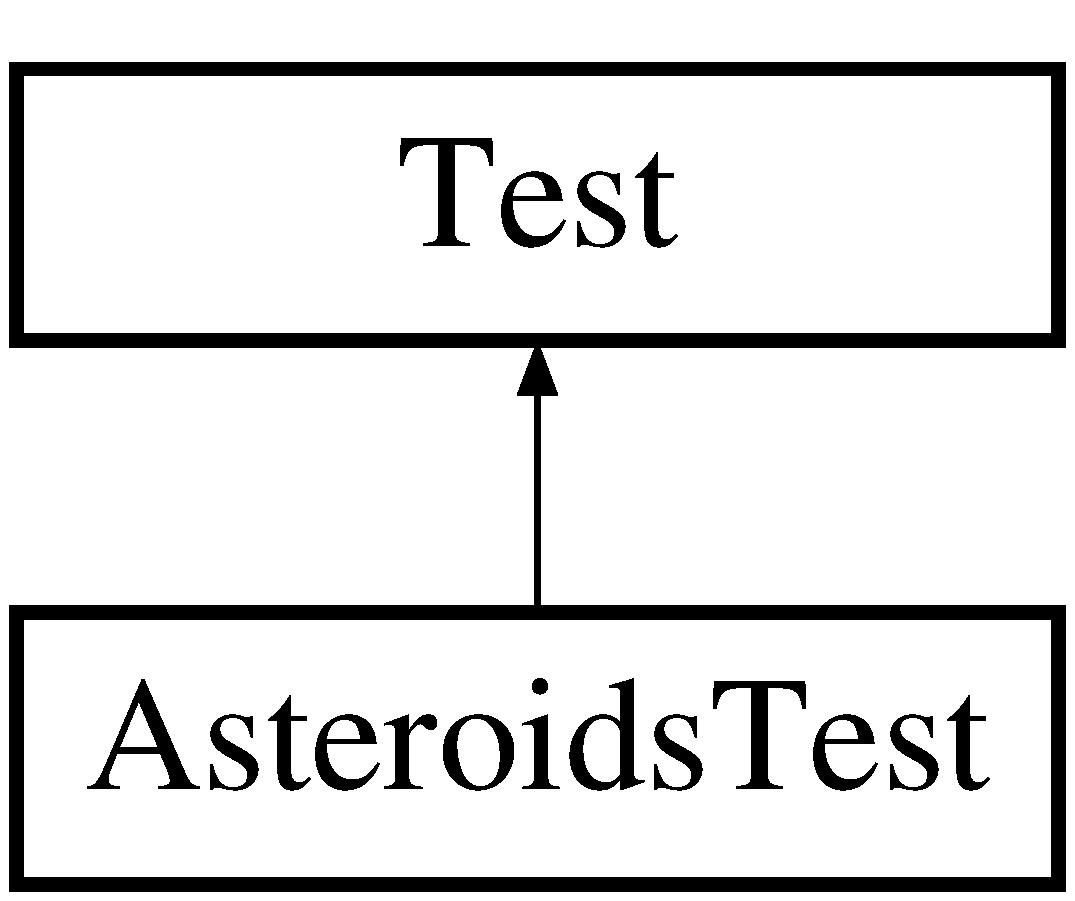
\includegraphics[height=2.000000cm]{classAsteroidsTest}
\end{center}
\end{figure}
\subsection*{Public Attributes}
\begin{DoxyCompactItemize}
\item 
\hyperlink{classGameRunner}{Game\+Runner} {\bfseries game\+Runner}\hypertarget{classAsteroidsTest_ad1af818c13b9401c5a92ca0da1f01620}{}\label{classAsteroidsTest_ad1af818c13b9401c5a92ca0da1f01620}

\item 
\hyperlink{classPythonRunner}{Python\+Runner} {\bfseries python\+Runner}\hypertarget{classAsteroidsTest_ac1d713b11a2c68611616e01251490770}{}\label{classAsteroidsTest_ac1d713b11a2c68611616e01251490770}

\end{DoxyCompactItemize}


The documentation for this class was generated from the following file\+:\begin{DoxyCompactItemize}
\item 
test/\+End\+To\+End\+Tests/Asteroid\+Collision\+End\+To\+End\+Tests.\+cpp\end{DoxyCompactItemize}

\hypertarget{classBadScaleArgumentException}{}\section{Bad\+Scale\+Argument\+Exception Class Reference}
\label{classBadScaleArgumentException}\index{Bad\+Scale\+Argument\+Exception@{Bad\+Scale\+Argument\+Exception}}
Inheritance diagram for Bad\+Scale\+Argument\+Exception\+:\begin{figure}[H]
\begin{center}
\leavevmode
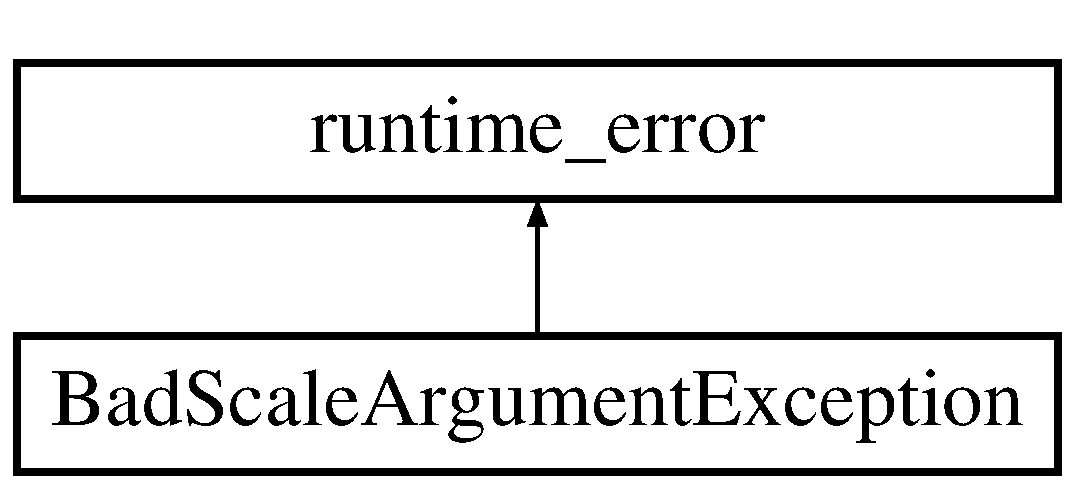
\includegraphics[height=2.000000cm]{classBadScaleArgumentException}
\end{center}
\end{figure}
\subsection*{Public Member Functions}
\begin{DoxyCompactItemize}
\item 
{\bfseries Bad\+Scale\+Argument\+Exception} (std\+::string text)\hypertarget{classBadScaleArgumentException_af354922bab2495deac08106e5d28e094}{}\label{classBadScaleArgumentException_af354922bab2495deac08106e5d28e094}

\end{DoxyCompactItemize}


The documentation for this class was generated from the following files\+:\begin{DoxyCompactItemize}
\item 
src/\+Model/exceptions/Bad\+Scale\+Argument\+Exception.\+h\item 
src/\+Model/exceptions/Bad\+Scale\+Argument\+Exception.\+cpp\end{DoxyCompactItemize}

\hypertarget{classBaseDrawablePrimitive}{}\section{Base\+Drawable\+Primitive Class Reference}
\label{classBaseDrawablePrimitive}\index{Base\+Drawable\+Primitive@{Base\+Drawable\+Primitive}}
Inheritance diagram for Base\+Drawable\+Primitive\+:\begin{figure}[H]
\begin{center}
\leavevmode
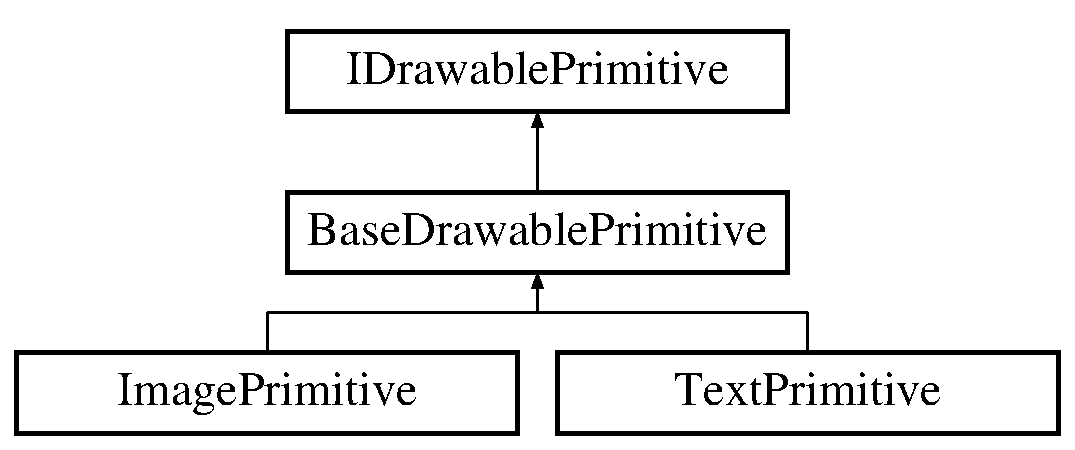
\includegraphics[height=3.000000cm]{classBaseDrawablePrimitive}
\end{center}
\end{figure}
\subsection*{Public Member Functions}
\begin{DoxyCompactItemize}
\item 
{\bfseries Base\+Drawable\+Primitive} (const \hyperlink{classPoint}{Point} \&position\+\_\+, const \hyperlink{classRotation}{Rotation} \&rotation\+\_\+, const \hyperlink{classScaleToScreen}{Scale\+To\+Screen} \&scale\+\_\+, const Actor\+Id \&id)\hypertarget{classBaseDrawablePrimitive_abd4da57d477eb4447f6326f0ed475873}{}\label{classBaseDrawablePrimitive_abd4da57d477eb4447f6326f0ed475873}

\item 
virtual \hyperlink{classPoint}{Point} {\bfseries get\+Position} () const \hypertarget{classBaseDrawablePrimitive_a4ed6d252dbe6ad464a22f18881b0fd01}{}\label{classBaseDrawablePrimitive_a4ed6d252dbe6ad464a22f18881b0fd01}

\item 
virtual void {\bfseries set\+Position} (\hyperlink{classPoint}{Point} new\+Position)\hypertarget{classBaseDrawablePrimitive_a09e32b302f1c861febcf5bc657015b11}{}\label{classBaseDrawablePrimitive_a09e32b302f1c861febcf5bc657015b11}

\item 
virtual \hyperlink{classRotation}{Rotation} {\bfseries get\+Rotation} () const \hypertarget{classBaseDrawablePrimitive_ae5d0896c69a2e8239f1cf3fea4b79c19}{}\label{classBaseDrawablePrimitive_ae5d0896c69a2e8239f1cf3fea4b79c19}

\item 
virtual void {\bfseries set\+Rotation} (\hyperlink{classRotation}{Rotation} rotation)\hypertarget{classBaseDrawablePrimitive_a79b5dbb3a600b0d96fd1d16c34d8d16b}{}\label{classBaseDrawablePrimitive_a79b5dbb3a600b0d96fd1d16c34d8d16b}

\item 
virtual \hyperlink{classScaleToScreen}{Scale\+To\+Screen} {\bfseries get\+Scale} () const \hypertarget{classBaseDrawablePrimitive_ab83c1407de521d94f95afc7b7b92cba3}{}\label{classBaseDrawablePrimitive_ab83c1407de521d94f95afc7b7b92cba3}

\item 
virtual Actor\+Id {\bfseries get\+Actor\+Id} () const \hypertarget{classBaseDrawablePrimitive_a01e16048f7aecfd38a8a32ed1db1f9d3}{}\label{classBaseDrawablePrimitive_a01e16048f7aecfd38a8a32ed1db1f9d3}

\end{DoxyCompactItemize}


The documentation for this class was generated from the following files\+:\begin{DoxyCompactItemize}
\item 
src/\+Model/\+Model\+Drawing/Base\+Drawable\+Primitive.\+h\item 
src/\+Model/\+Model\+Drawing/Base\+Drawable\+Primitive.\+cpp\end{DoxyCompactItemize}

\hypertarget{classBorderIndicatorComponent}{}\section{Border\+Indicator\+Component Class Reference}
\label{classBorderIndicatorComponent}\index{Border\+Indicator\+Component@{Border\+Indicator\+Component}}
Inheritance diagram for Border\+Indicator\+Component\+:\begin{figure}[H]
\begin{center}
\leavevmode
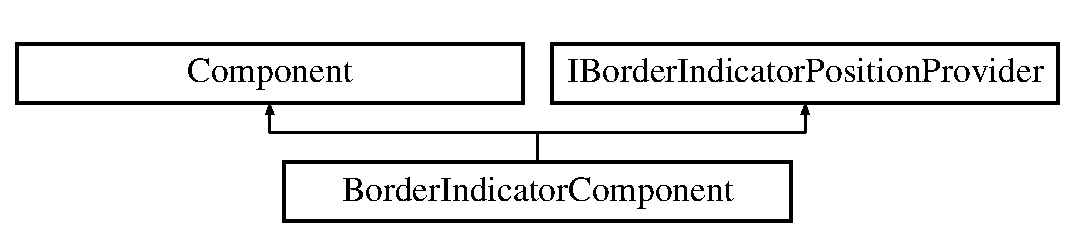
\includegraphics[height=2.000000cm]{classBorderIndicatorComponent}
\end{center}
\end{figure}
\subsection*{Public Member Functions}
\begin{DoxyCompactItemize}
\item 
virtual \hyperlink{classPoint}{Point} {\bfseries get\+Border\+Indicator\+Position} () override\hypertarget{classBorderIndicatorComponent_aab0da56e04ed52b0fb2671a5a5b8e890}{}\label{classBorderIndicatorComponent_aab0da56e04ed52b0fb2671a5a5b8e890}

\item 
{\bfseries Border\+Indicator\+Component} (\hyperlink{classGameConfiguration}{Game\+Configuration} \&configuration, std\+::shared\+\_\+ptr$<$ \hyperlink{classIInputStateProvider}{I\+Input\+State\+Provider} $>$ input\+State\+Provider)\hypertarget{classBorderIndicatorComponent_a5c2510b41aefd2c314a6fd3521c73ca2}{}\label{classBorderIndicatorComponent_a5c2510b41aefd2c314a6fd3521c73ca2}

\item 
void {\bfseries On\+Start} (\hyperlink{classIActor}{I\+Actor} \&actor)\hypertarget{classBorderIndicatorComponent_ab3ec2039eacd57b7e69a718cfb2b1810}{}\label{classBorderIndicatorComponent_ab3ec2039eacd57b7e69a718cfb2b1810}

\item 
void {\bfseries On\+Update} ()\hypertarget{classBorderIndicatorComponent_a749a22b485f4a361203bf7d7eee7e728}{}\label{classBorderIndicatorComponent_a749a22b485f4a361203bf7d7eee7e728}

\end{DoxyCompactItemize}


The documentation for this class was generated from the following files\+:\begin{DoxyCompactItemize}
\item 
src/\+Model/\+Actors/second\+Player/Border\+Indicator\+Component.\+h\item 
src/\+Model/\+Actors/second\+Player/Border\+Indicator\+Component.\+cpp\end{DoxyCompactItemize}

\hypertarget{classBoundariesDuplicationsDrawingSystem}{}\section{Boundaries\+Duplications\+Drawing\+System Class Reference}
\label{classBoundariesDuplicationsDrawingSystem}\index{Boundaries\+Duplications\+Drawing\+System@{Boundaries\+Duplications\+Drawing\+System}}
Inheritance diagram for Boundaries\+Duplications\+Drawing\+System\+:\begin{figure}[H]
\begin{center}
\leavevmode
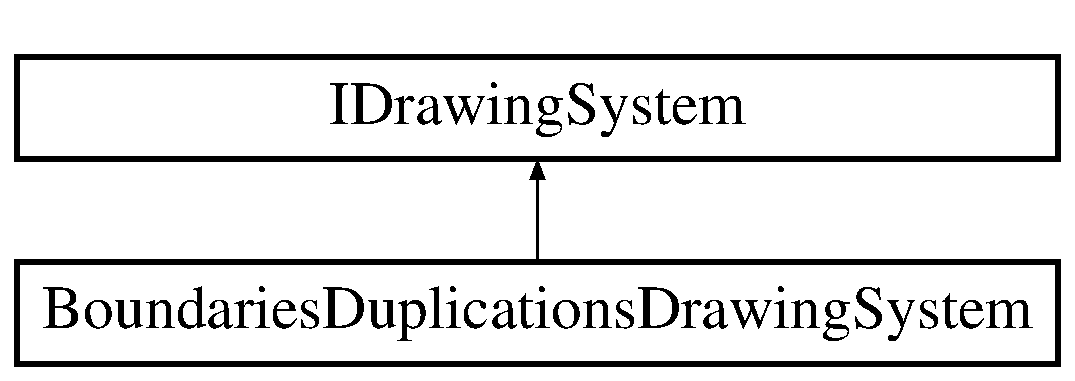
\includegraphics[height=2.000000cm]{classBoundariesDuplicationsDrawingSystem}
\end{center}
\end{figure}
\subsection*{Public Member Functions}
\begin{DoxyCompactItemize}
\item 
{\bfseries Boundaries\+Duplications\+Drawing\+System} (\hyperlink{classIDrawingSystem}{I\+Drawing\+System} \&normal\+Drawing\+System, \hyperlink{classGameConfiguration}{Game\+Configuration} \&configuration)\hypertarget{classBoundariesDuplicationsDrawingSystem_aa7e9dc7d958875a3ff5be36220772b81}{}\label{classBoundariesDuplicationsDrawingSystem_aa7e9dc7d958875a3ff5be36220772b81}

\item 
virtual void {\bfseries draw\+Image} (Image\+Primitive\+Type type, \hyperlink{classPoint}{Point} position, \hyperlink{classRotation}{Rotation} rotation, \hyperlink{classScaleToScreen}{Scale\+To\+Screen} scale, Actor\+Id actor\+Id)\hypertarget{classBoundariesDuplicationsDrawingSystem_aaa9f57dbe6ffca81e36c9f14203cf4f8}{}\label{classBoundariesDuplicationsDrawingSystem_aaa9f57dbe6ffca81e36c9f14203cf4f8}

\item 
virtual void {\bfseries draw\+Text} (std\+::string text\+Value, \hyperlink{classPoint}{Point} position, Actor\+Id actor\+Id)\hypertarget{classBoundariesDuplicationsDrawingSystem_ac9785d4966c65f6c33db11d7f1cc401f}{}\label{classBoundariesDuplicationsDrawingSystem_ac9785d4966c65f6c33db11d7f1cc401f}

\item 
virtual void {\bfseries add\+Removed\+Actor\+Id} (Actor\+Id id) override\hypertarget{classBoundariesDuplicationsDrawingSystem_ad3779a653b21d84b68d190d38176a1cc}{}\label{classBoundariesDuplicationsDrawingSystem_ad3779a653b21d84b68d190d38176a1cc}

\end{DoxyCompactItemize}


The documentation for this class was generated from the following files\+:\begin{DoxyCompactItemize}
\item 
src/\+Model/\+Model\+Drawing/Boundaries\+Duplications\+Drawing\+System.\+h\item 
src/\+Model/\+Model\+Drawing/Boundaries\+Duplications\+Drawing\+System.\+cpp\end{DoxyCompactItemize}

\hypertarget{classBox2dCollisionsComponent}{}\section{Box2d\+Collisions\+Component Class Reference}
\label{classBox2dCollisionsComponent}\index{Box2d\+Collisions\+Component@{Box2d\+Collisions\+Component}}
Inheritance diagram for Box2d\+Collisions\+Component\+:\begin{figure}[H]
\begin{center}
\leavevmode
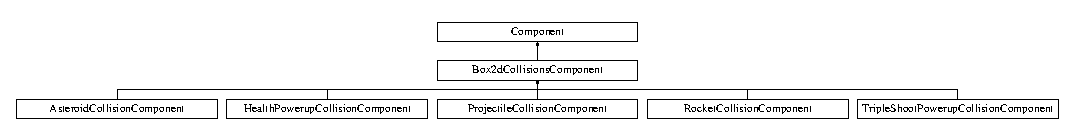
\includegraphics[height=1.371429cm]{classBox2dCollisionsComponent}
\end{center}
\end{figure}
\subsection*{Public Member Functions}
\begin{DoxyCompactItemize}
\item 
{\bfseries Box2d\+Collisions\+Component} (\hyperlink{classContactComponentsContainer}{Contact\+Components\+Container} \&contact\+Container)\hypertarget{classBox2dCollisionsComponent_aa473347ad04a40bf29e72991da00fea4}{}\label{classBox2dCollisionsComponent_aa473347ad04a40bf29e72991da00fea4}

\item 
void {\bfseries On\+Start} (\hyperlink{classIActor}{I\+Actor} \&actor)\hypertarget{classBox2dCollisionsComponent_a6fe4bd1e26cc06369f0d167b64de1c05}{}\label{classBox2dCollisionsComponent_a6fe4bd1e26cc06369f0d167b64de1c05}

\item 
void {\bfseries On\+Stop} ()\hypertarget{classBox2dCollisionsComponent_ab54794a4252120907010ee9c5629faed}{}\label{classBox2dCollisionsComponent_ab54794a4252120907010ee9c5629faed}

\item 
void {\bfseries On\+Update} ()\hypertarget{classBox2dCollisionsComponent_a2e5ac66dfe25b7e02865114718114378}{}\label{classBox2dCollisionsComponent_a2e5ac66dfe25b7e02865114718114378}

\item 
void {\bfseries add\+Colision} (\hyperlink{structCollisionData}{Collision\+Data} data)\hypertarget{classBox2dCollisionsComponent_a93ca668f40bb24d58d9e22837cabcf48}{}\label{classBox2dCollisionsComponent_a93ca668f40bb24d58d9e22837cabcf48}

\end{DoxyCompactItemize}
\subsection*{Protected Attributes}
\begin{DoxyCompactItemize}
\item 
std\+::shared\+\_\+ptr$<$ \hyperlink{classBox2dComponent}{Box2d\+Component} $>$ {\bfseries box2d\+Component\+\_\+}\hypertarget{classBox2dCollisionsComponent_ac0dca57c3b49a8ac6cd5a09413b2532c}{}\label{classBox2dCollisionsComponent_ac0dca57c3b49a8ac6cd5a09413b2532c}

\end{DoxyCompactItemize}


The documentation for this class was generated from the following files\+:\begin{DoxyCompactItemize}
\item 
src/\+Model/collisions/Box2d\+Collisions\+Component.\+h\item 
src/\+Model/collisions/Box2d\+Collisions\+Component.\+cpp\end{DoxyCompactItemize}

\hypertarget{classBox2dComponent}{}\section{Box2d\+Component Class Reference}
\label{classBox2dComponent}\index{Box2d\+Component@{Box2d\+Component}}
Inheritance diagram for Box2d\+Component\+:\begin{figure}[H]
\begin{center}
\leavevmode
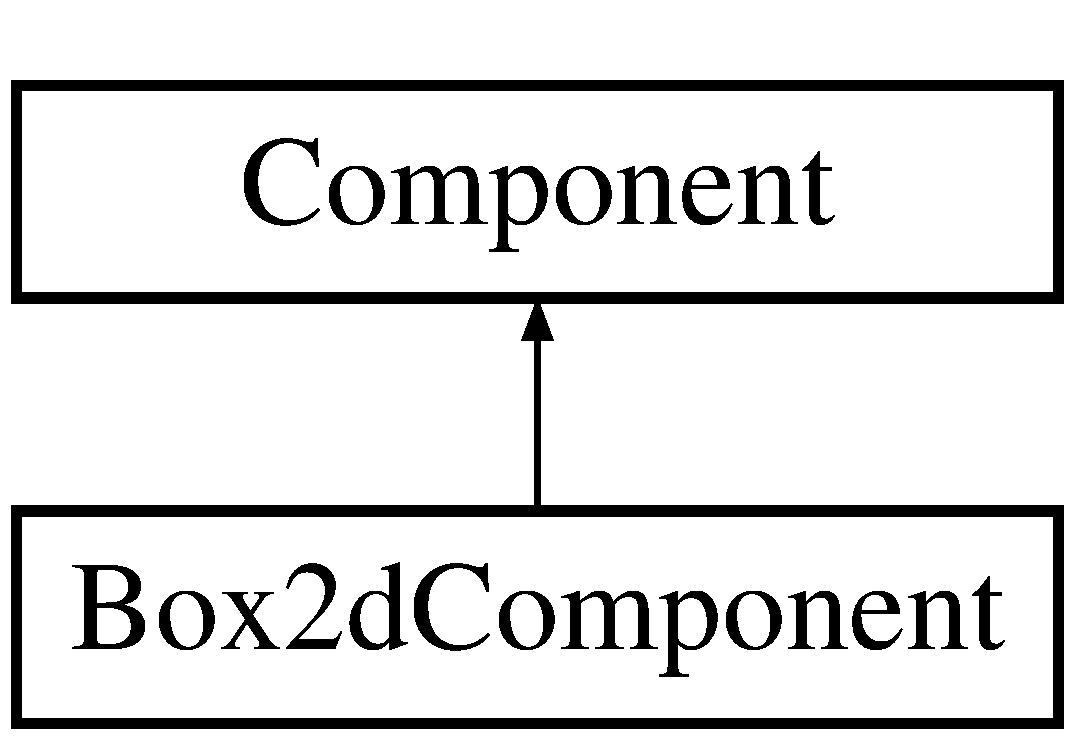
\includegraphics[height=2.000000cm]{classBox2dComponent}
\end{center}
\end{figure}
\subsection*{Public Member Functions}
\begin{DoxyCompactItemize}
\item 
{\bfseries Box2d\+Component} (std\+::shared\+\_\+ptr$<$ \hyperlink{classBox2DService}{Box2\+D\+Service} $>$ box2d\+Service, \hyperlink{classGameConfiguration}{Game\+Configuration} \&configurable\+Values, std\+::shared\+\_\+ptr$<$ \hyperlink{classBox2dObject}{Box2d\+Object} $>$ rocket\+Box2d\+Object)\hypertarget{classBox2dComponent_a7287159031753cbfeb253cffe220c46c}{}\label{classBox2dComponent_a7287159031753cbfeb253cffe220c46c}

\item 
virtual void {\bfseries On\+Start} (\hyperlink{classIActor}{I\+Actor} \&actor)\hypertarget{classBox2dComponent_a4ffa4328e50443a258226cbd5c92fec3}{}\label{classBox2dComponent_a4ffa4328e50443a258226cbd5c92fec3}

\item 
virtual void {\bfseries On\+Update} ()\hypertarget{classBox2dComponent_a24767c8d67bec9e557038330bb136958}{}\label{classBox2dComponent_a24767c8d67bec9e557038330bb136958}

\item 
virtual void {\bfseries On\+Stop} ()\hypertarget{classBox2dComponent_ae91ad9fd1ac4a0950b01e7ab12bf6d7e}{}\label{classBox2dComponent_ae91ad9fd1ac4a0950b01e7ab12bf6d7e}

\item 
void {\bfseries apply\+Force} (\hyperlink{classPoint}{Point} force\+Vector)\hypertarget{classBox2dComponent_a3180efda44919c4f37aa83e93b96a036}{}\label{classBox2dComponent_a3180efda44919c4f37aa83e93b96a036}

\item 
void {\bfseries apply\+Torque} (double torque)\hypertarget{classBox2dComponent_af32c4ae582ce53333352cea32cf316ba}{}\label{classBox2dComponent_af32c4ae582ce53333352cea32cf316ba}

\item 
void {\bfseries set\+Position} (double x, double y)\hypertarget{classBox2dComponent_a51a6d470f67f542e05403c1e7f9bb76f}{}\label{classBox2dComponent_a51a6d470f67f542e05403c1e7f9bb76f}

\item 
void {\bfseries set\+Rotation} (double rotation)\hypertarget{classBox2dComponent_a2ff4ab8dc5eed26824ae13e3e305b414}{}\label{classBox2dComponent_a2ff4ab8dc5eed26824ae13e3e305b414}

\item 
void {\bfseries apply\+Lineral\+Impulse} (\hyperlink{classPoint}{Point} vec)\hypertarget{classBox2dComponent_a222c329dd4b78ba416b37e23046cc729}{}\label{classBox2dComponent_a222c329dd4b78ba416b37e23046cc729}

\item 
void {\bfseries apply\+Angular\+Impulse} (double value)\hypertarget{classBox2dComponent_aa1be5c7330ce571911b2a642aebeff7b}{}\label{classBox2dComponent_aa1be5c7330ce571911b2a642aebeff7b}

\item 
void {\bfseries Set\+Lineral\+Velocity} (\hyperlink{classPoint}{Point} speed\+Vector)\hypertarget{classBox2dComponent_a853f5c32d29169a4ec13c1d92ed9eb02}{}\label{classBox2dComponent_a853f5c32d29169a4ec13c1d92ed9eb02}

\item 
void {\bfseries Set\+Angular\+Velocity} (double velocity)\hypertarget{classBox2dComponent_a7093fe0c26442b394c487c892d601891}{}\label{classBox2dComponent_a7093fe0c26442b394c487c892d601891}

\item 
\hyperlink{classPoint}{Point} {\bfseries get\+Lineral\+Velocity} ()\hypertarget{classBox2dComponent_a6d2848cfe0e699038274c549993def47}{}\label{classBox2dComponent_a6d2848cfe0e699038274c549993def47}

\item 
b2\+Body $\ast$ {\bfseries get\+Body} ()\hypertarget{classBox2dComponent_a73685bf084d8043f3c771b1a21f90b3a}{}\label{classBox2dComponent_a73685bf084d8043f3c771b1a21f90b3a}

\item 
double {\bfseries get\+Mass} ()\hypertarget{classBox2dComponent_a10e6cae953fa1382d9d2adad9509b16e}{}\label{classBox2dComponent_a10e6cae953fa1382d9d2adad9509b16e}

\item 
\hyperlink{classPoint}{Point} {\bfseries get\+Box\+Size} ()\hypertarget{classBox2dComponent_a7e00a4971f000feec4f1824dfd1d171e}{}\label{classBox2dComponent_a7e00a4971f000feec4f1824dfd1d171e}

\end{DoxyCompactItemize}


The documentation for this class was generated from the following files\+:\begin{DoxyCompactItemize}
\item 
src/\+Model/\+Actors/\+Rocket/Box2d\+Component.\+h\item 
src/\+Model/\+Actors/\+Rocket/Box2d\+Component.\+cpp\end{DoxyCompactItemize}

\hypertarget{classBox2dObject}{}\section{Box2d\+Object Class Reference}
\label{classBox2dObject}\index{Box2d\+Object@{Box2d\+Object}}
\subsection*{Public Member Functions}
\begin{DoxyCompactItemize}
\item 
{\bfseries Box2d\+Object} (b2\+Body\+Def def, std\+::vector$<$ b2\+Fixture\+Def $>$ fixture\+Def\+Vec, double mass, \hyperlink{classPoint}{Point} box\+Size)\hypertarget{classBox2dObject_ac710f47a1f53fea5e7e8328e1db48969}{}\label{classBox2dObject_ac710f47a1f53fea5e7e8328e1db48969}

\item 
const b2\+Body\+Def $\ast$ {\bfseries get\+Def} ()\hypertarget{classBox2dObject_ab4eee398bdfc614e2610f5e659dca9f5}{}\label{classBox2dObject_ab4eee398bdfc614e2610f5e659dca9f5}

\item 
void {\bfseries set\+Body\+And\+Create\+Fixtures} (b2\+Body $\ast$body)\hypertarget{classBox2dObject_aa8d38b6de3d0c7b389b28a59e68aec24}{}\label{classBox2dObject_aa8d38b6de3d0c7b389b28a59e68aec24}

\item 
b2\+Body $\ast$ {\bfseries get\+Body} ()\hypertarget{classBox2dObject_af91c5d9ad12a410549b4b271e78d3080}{}\label{classBox2dObject_af91c5d9ad12a410549b4b271e78d3080}

\item 
std\+::vector$<$ b2\+Fixture $\ast$ $>$ {\bfseries get\+Fixtures} ()\hypertarget{classBox2dObject_ab9143129c22eddc6181d3b61e1b6760c}{}\label{classBox2dObject_ab9143129c22eddc6181d3b61e1b6760c}

\item 
double {\bfseries get\+Mass} ()\hypertarget{classBox2dObject_a799708a749a48b323132417d61badbce}{}\label{classBox2dObject_a799708a749a48b323132417d61badbce}

\item 
\hyperlink{classPoint}{Point} {\bfseries get\+Box\+Size} ()\hypertarget{classBox2dObject_ab141066294257405dd26a8d1515b0ff8}{}\label{classBox2dObject_ab141066294257405dd26a8d1515b0ff8}

\end{DoxyCompactItemize}


The documentation for this class was generated from the following files\+:\begin{DoxyCompactItemize}
\item 
src/\+Model/box2d/Box2d\+Object.\+h\item 
src/\+Model/box2d/Box2d\+Object.\+cpp\end{DoxyCompactItemize}

\hypertarget{classBox2dObjectsContainer}{}\section{Box2d\+Objects\+Container Class Reference}
\label{classBox2dObjectsContainer}\index{Box2d\+Objects\+Container@{Box2d\+Objects\+Container}}
\subsection*{Public Member Functions}
\begin{DoxyCompactItemize}
\item 
{\bfseries Box2d\+Objects\+Container} (\hyperlink{classImageScalesContainer}{Image\+Scales\+Container} \&image\+Scales\+Container, \hyperlink{classGameConfiguration}{Game\+Configuration} \&game\+Configuration)\hypertarget{classBox2dObjectsContainer_aea1ca4c4acceff6bf31d079a94acc948}{}\label{classBox2dObjectsContainer_aea1ca4c4acceff6bf31d079a94acc948}

\item 
std\+::shared\+\_\+ptr$<$ \hyperlink{classBox2dObject}{Box2d\+Object} $>$ {\bfseries get\+Rocket\+Object} ()\hypertarget{classBox2dObjectsContainer_a074e14b69d50fd592e661ca4ecc35b8c}{}\label{classBox2dObjectsContainer_a074e14b69d50fd592e661ca4ecc35b8c}

\item 
std\+::shared\+\_\+ptr$<$ \hyperlink{classBox2dObject}{Box2d\+Object} $>$ {\bfseries get\+Asteriod\+Object} (double size)\hypertarget{classBox2dObjectsContainer_afe57a3e2e321bd411ab585a7f3ea262b}{}\label{classBox2dObjectsContainer_afe57a3e2e321bd411ab585a7f3ea262b}

\item 
std\+::shared\+\_\+ptr$<$ \hyperlink{classBox2dObject}{Box2d\+Object} $>$ {\bfseries get\+Projectile\+Object} ()\hypertarget{classBox2dObjectsContainer_acaba2899c36dde3216840df186bf08f3}{}\label{classBox2dObjectsContainer_acaba2899c36dde3216840df186bf08f3}

\item 
std\+::shared\+\_\+ptr$<$ \hyperlink{classBox2dObject}{Box2d\+Object} $>$ {\bfseries get\+Powerup\+Object} ()\hypertarget{classBox2dObjectsContainer_a23006c7f8699cbfb50ce45664259858a}{}\label{classBox2dObjectsContainer_a23006c7f8699cbfb50ce45664259858a}

\end{DoxyCompactItemize}


The documentation for this class was generated from the following files\+:\begin{DoxyCompactItemize}
\item 
src/\+Model/box2d/Box2d\+Objects\+Container.\+h\item 
src/\+Model/box2d/Box2d\+Objects\+Container.\+cpp\end{DoxyCompactItemize}

\hypertarget{classBox2DService}{}\section{Box2\+D\+Service Class Reference}
\label{classBox2DService}\index{Box2\+D\+Service@{Box2\+D\+Service}}
Inheritance diagram for Box2\+D\+Service\+:\begin{figure}[H]
\begin{center}
\leavevmode
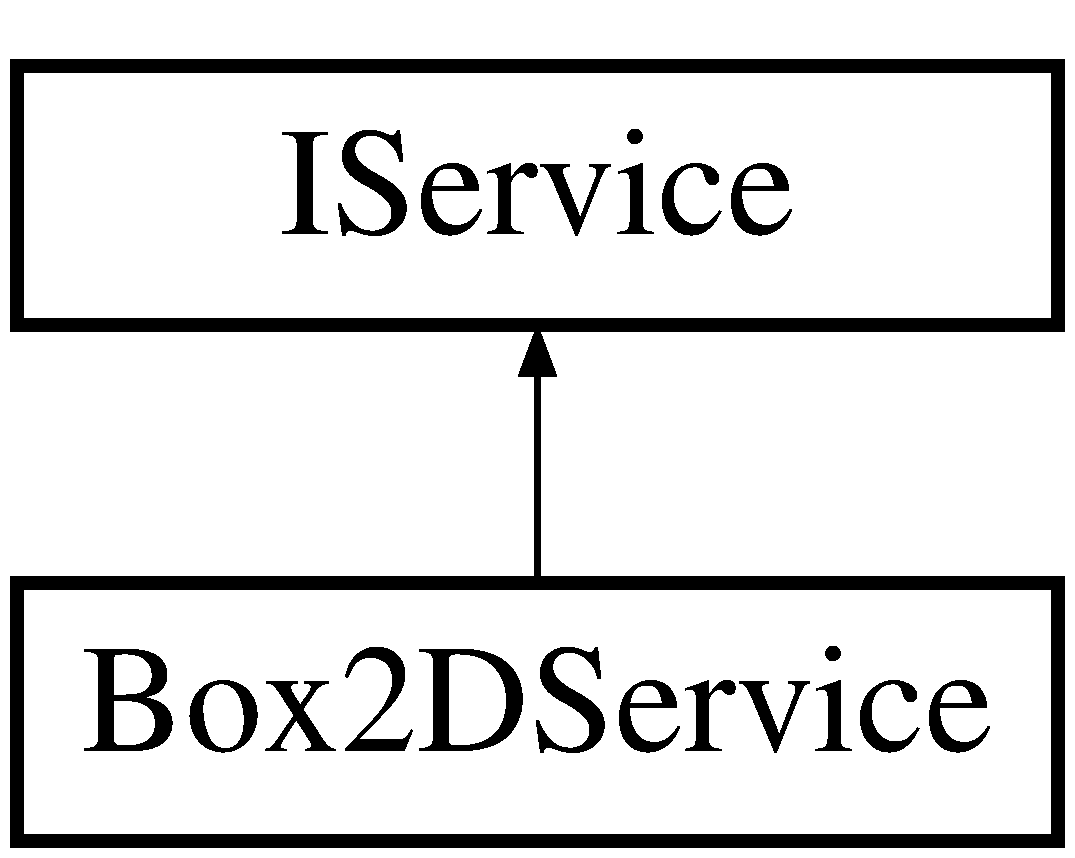
\includegraphics[height=2.000000cm]{classBox2DService}
\end{center}
\end{figure}
\subsection*{Public Member Functions}
\begin{DoxyCompactItemize}
\item 
{\bfseries Box2\+D\+Service} (\hyperlink{classMyContactListener}{My\+Contact\+Listener} $\ast$contact\+Listener)\hypertarget{classBox2DService_a3ca3204851a4e6eae4aacde6617c4818}{}\label{classBox2DService_a3ca3204851a4e6eae4aacde6617c4818}

\item 
void {\bfseries add\+Object} (std\+::shared\+\_\+ptr$<$ \hyperlink{classBox2dObject}{Box2d\+Object} $>$ object)\hypertarget{classBox2DService_a6faffb2b4439c5ed4f49e5fa3785f4b8}{}\label{classBox2DService_a6faffb2b4439c5ed4f49e5fa3785f4b8}

\item 
void {\bfseries remove\+Object} (std\+::shared\+\_\+ptr$<$ \hyperlink{classBox2dObject}{Box2d\+Object} $>$ object)\hypertarget{classBox2DService_a4009a4f322e0be198de299168c650d54}{}\label{classBox2DService_a4009a4f322e0be198de299168c650d54}

\item 
virtual void {\bfseries On\+Update} ()\hypertarget{classBox2DService_ad09f15234a24d28af6b017f94efbb956}{}\label{classBox2DService_ad09f15234a24d28af6b017f94efbb956}

\item 
void {\bfseries turn\+Off\+Simulation} ()\hypertarget{classBox2DService_a9b5e6211e8c743d71d84a35527801a6c}{}\label{classBox2DService_a9b5e6211e8c743d71d84a35527801a6c}

\item 
void {\bfseries turn\+On\+Simulation} ()\hypertarget{classBox2DService_a309d8a33b083af6f672d7b528772c307}{}\label{classBox2DService_a309d8a33b083af6f672d7b528772c307}

\end{DoxyCompactItemize}


The documentation for this class was generated from the following files\+:\begin{DoxyCompactItemize}
\item 
src/\+Model/box2d/Box2\+D\+Service.\+h\item 
src/\+Model/box2d/Box2\+D\+Service.\+cpp\end{DoxyCompactItemize}

\hypertarget{classC1}{}\section{C1 Class Reference}
\label{classC1}\index{C1@{C1}}
Inheritance diagram for C1\+:\begin{figure}[H]
\begin{center}
\leavevmode
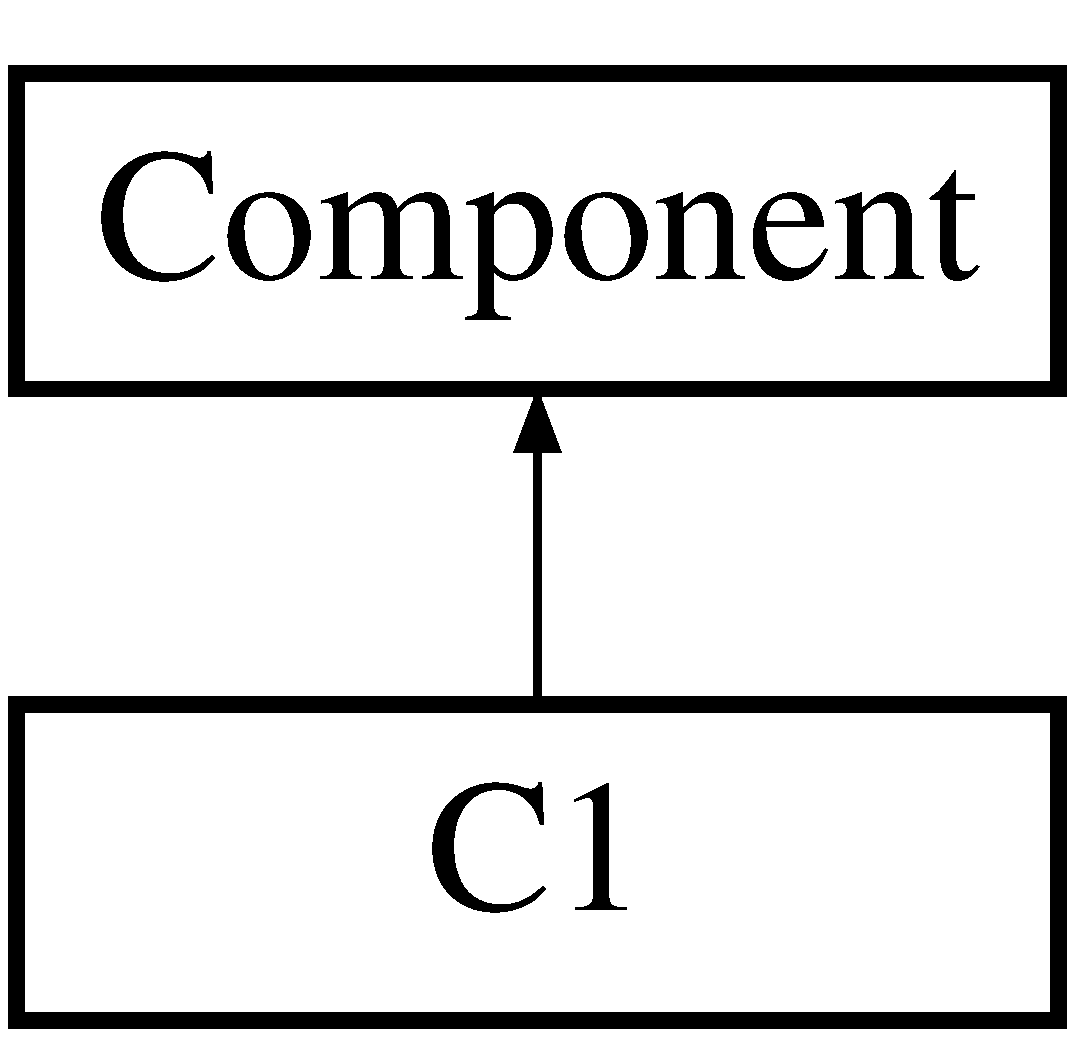
\includegraphics[height=2.000000cm]{classC1}
\end{center}
\end{figure}
\subsection*{Additional Inherited Members}


The documentation for this class was generated from the following file\+:\begin{DoxyCompactItemize}
\item 
test/Component\+Type\+Information\+Test.\+cpp\end{DoxyCompactItemize}

\hypertarget{classC2}{}\section{C2 Class Reference}
\label{classC2}\index{C2@{C2}}
Inheritance diagram for C2\+:\begin{figure}[H]
\begin{center}
\leavevmode
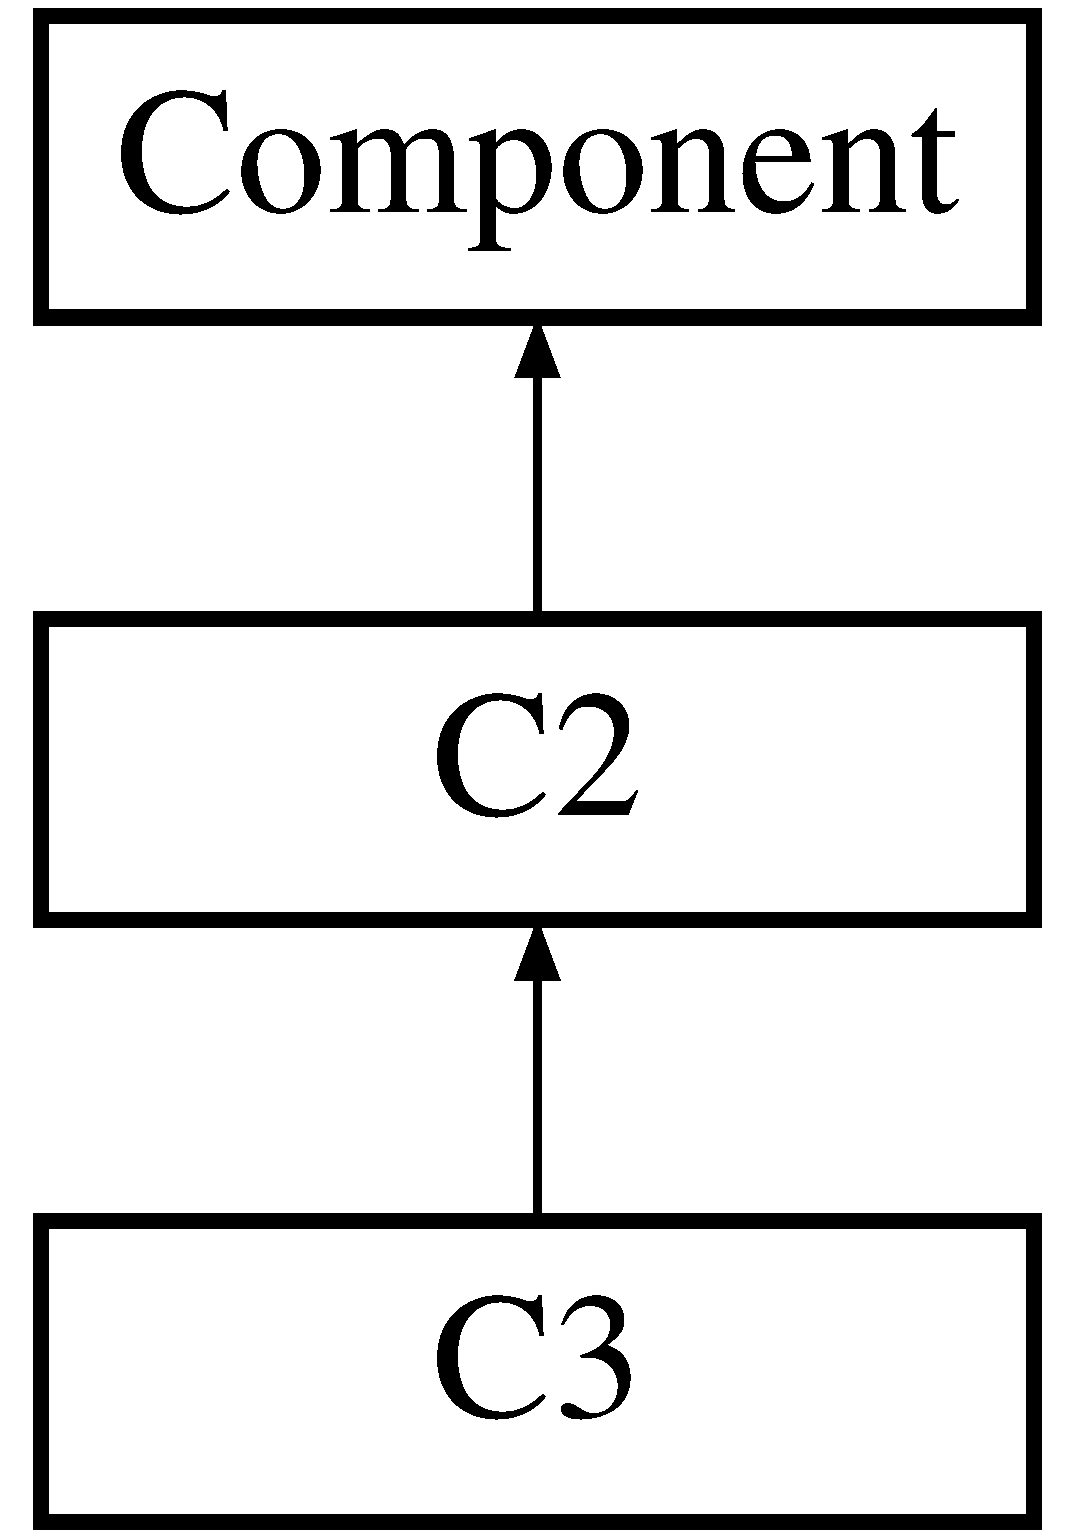
\includegraphics[height=3.000000cm]{classC2}
\end{center}
\end{figure}
\subsection*{Additional Inherited Members}


The documentation for this class was generated from the following file\+:\begin{DoxyCompactItemize}
\item 
test/Component\+Type\+Information\+Test.\+cpp\end{DoxyCompactItemize}

\hypertarget{classC3}{}\section{C3 Class Reference}
\label{classC3}\index{C3@{C3}}
Inheritance diagram for C3\+:\begin{figure}[H]
\begin{center}
\leavevmode
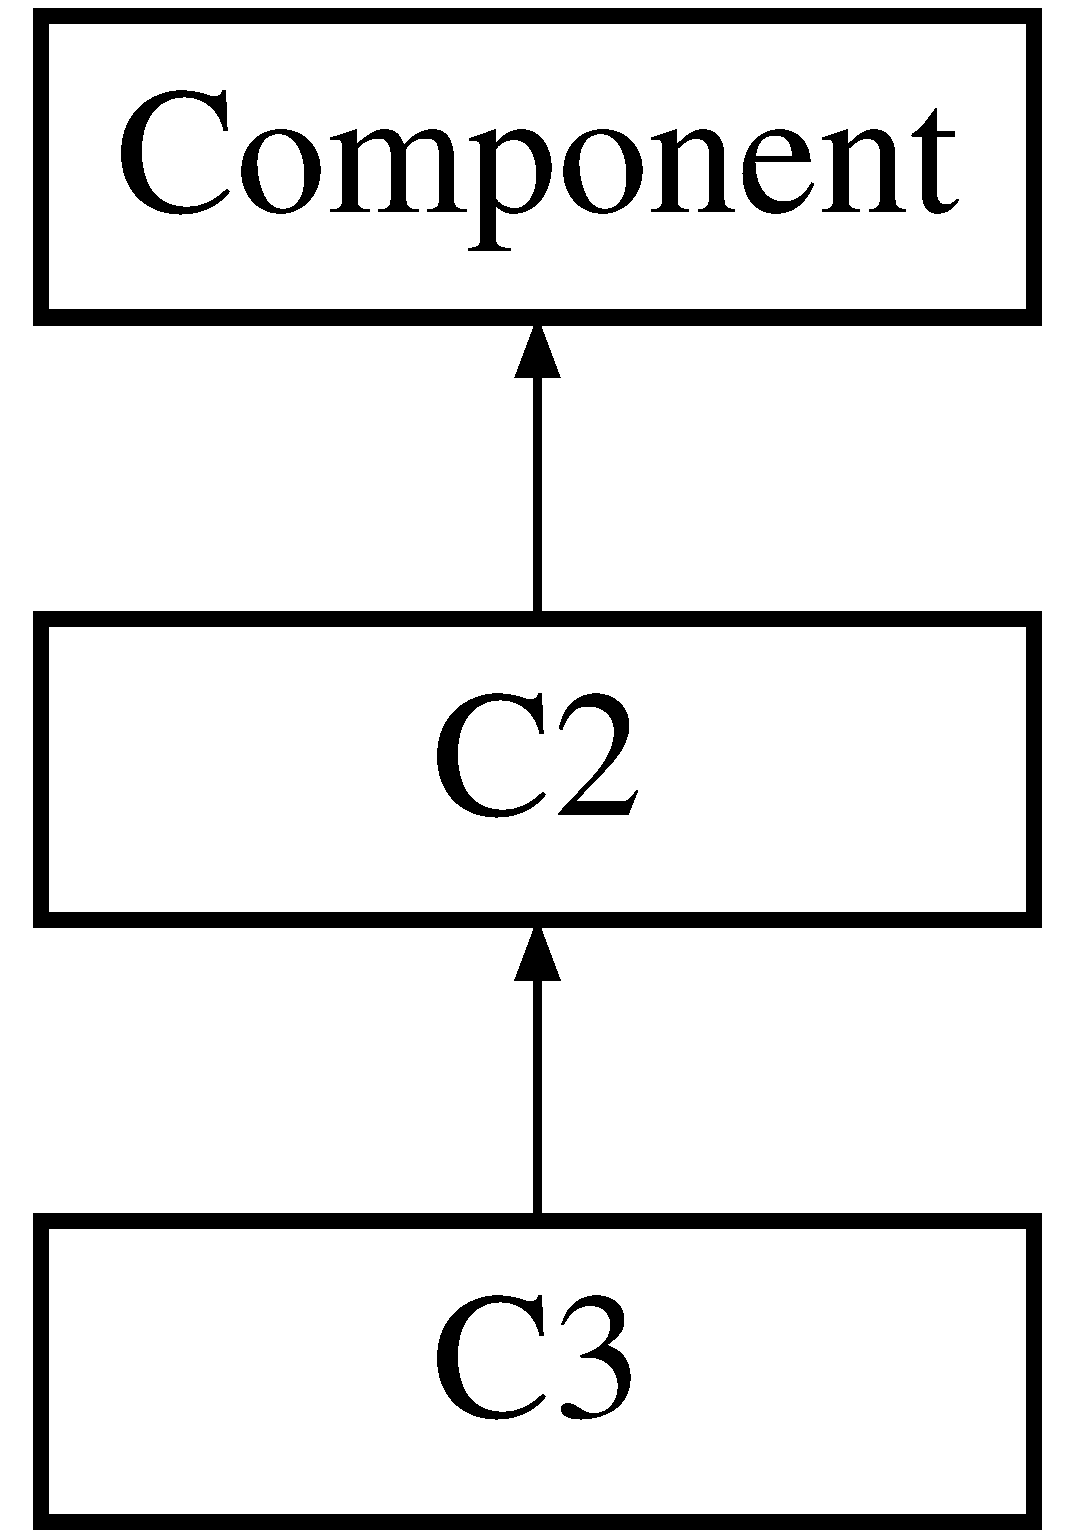
\includegraphics[height=3.000000cm]{classC3}
\end{center}
\end{figure}
\subsection*{Additional Inherited Members}


The documentation for this class was generated from the following file\+:\begin{DoxyCompactItemize}
\item 
test/Component\+Type\+Information\+Test.\+cpp\end{DoxyCompactItemize}

\hypertarget{structCollisionData}{}\section{Collision\+Data Struct Reference}
\label{structCollisionData}\index{Collision\+Data@{Collision\+Data}}
\subsection*{Public Member Functions}
\begin{DoxyCompactItemize}
\item 
{\bfseries Collision\+Data} (const Collision\+Group collision\+Group, double impulse\+Value, b2\+Fixture $\ast$other\+Contacter\+Fixture)\hypertarget{structCollisionData_a027fba5829b51a5079021c30381f11ca}{}\label{structCollisionData_a027fba5829b51a5079021c30381f11ca}

\end{DoxyCompactItemize}
\subsection*{Public Attributes}
\begin{DoxyCompactItemize}
\item 
Collision\+Group {\bfseries collision\+Group}\hypertarget{structCollisionData_a49804c0a69aa20483f6506c326837472}{}\label{structCollisionData_a49804c0a69aa20483f6506c326837472}

\item 
double {\bfseries impulse\+Value}\hypertarget{structCollisionData_adeb5b92a90ea55f87afa2df1263354cd}{}\label{structCollisionData_adeb5b92a90ea55f87afa2df1263354cd}

\item 
b2\+Fixture $\ast$ {\bfseries other\+Contacter\+Fixture}\hypertarget{structCollisionData_a9a1d6f8a1814eb34a8f16239d189a02f}{}\label{structCollisionData_a9a1d6f8a1814eb34a8f16239d189a02f}

\end{DoxyCompactItemize}


The documentation for this struct was generated from the following file\+:\begin{DoxyCompactItemize}
\item 
src/\+Model/collisions/Collision\+Data.\+h\end{DoxyCompactItemize}

\hypertarget{classCollisionGroupsData}{}\section{Collision\+Groups\+Data Class Reference}
\label{classCollisionGroupsData}\index{Collision\+Groups\+Data@{Collision\+Groups\+Data}}
\subsection*{Public Member Functions}
\begin{DoxyCompactItemize}
\item 
{\bfseries Collision\+Groups\+Data} (unsigned int category\+Bits, unsigned int mask\+Bits)\hypertarget{classCollisionGroupsData_a218c0061136e6e2e93db3c958b9bbc00}{}\label{classCollisionGroupsData_a218c0061136e6e2e93db3c958b9bbc00}

\end{DoxyCompactItemize}
\subsection*{Static Public Member Functions}
\begin{DoxyCompactItemize}
\item 
static \hyperlink{classCollisionGroupsData}{Collision\+Groups\+Data} {\bfseries get\+Asteroid\+Data} ()\hypertarget{classCollisionGroupsData_a86d651338c81b5527eb0198943cc668f}{}\label{classCollisionGroupsData_a86d651338c81b5527eb0198943cc668f}

\item 
static \hyperlink{classCollisionGroupsData}{Collision\+Groups\+Data} {\bfseries get\+Rocket\+Data} ()\hypertarget{classCollisionGroupsData_aec98d202dd50071efc45dcf08510fa73}{}\label{classCollisionGroupsData_aec98d202dd50071efc45dcf08510fa73}

\item 
static \hyperlink{classCollisionGroupsData}{Collision\+Groups\+Data} {\bfseries get\+Projectile\+Data} ()\hypertarget{classCollisionGroupsData_ac6cd27485f1aca9d5c1036cb819eb85b}{}\label{classCollisionGroupsData_ac6cd27485f1aca9d5c1036cb819eb85b}

\item 
static \hyperlink{classCollisionGroupsData}{Collision\+Groups\+Data} {\bfseries get\+Powerup\+Data} ()\hypertarget{classCollisionGroupsData_a3cded86803ba1591944e579978c6939d}{}\label{classCollisionGroupsData_a3cded86803ba1591944e579978c6939d}

\end{DoxyCompactItemize}
\subsection*{Public Attributes}
\begin{DoxyCompactItemize}
\item 
unsigned short {\bfseries category\+Bits\+\_\+}\hypertarget{classCollisionGroupsData_a2943a728bc5a2c3e054173ebc94e2e2a}{}\label{classCollisionGroupsData_a2943a728bc5a2c3e054173ebc94e2e2a}

\item 
unsigned short {\bfseries mask\+Bits\+\_\+}\hypertarget{classCollisionGroupsData_a5f3d1acf7a7c1541429c55aeda69a132}{}\label{classCollisionGroupsData_a5f3d1acf7a7c1541429c55aeda69a132}

\end{DoxyCompactItemize}


The documentation for this class was generated from the following files\+:\begin{DoxyCompactItemize}
\item 
src/\+Model/collisions/Collision\+Groups\+Data.\+h\item 
src/\+Model/collisions/Collision\+Groups\+Data.\+cpp\end{DoxyCompactItemize}

\hypertarget{classCommonTypesVisualizer}{}\section{Common\+Types\+Visualizer Class Reference}
\label{classCommonTypesVisualizer}\index{Common\+Types\+Visualizer@{Common\+Types\+Visualizer}}
Inheritance diagram for Common\+Types\+Visualizer\+:\begin{figure}[H]
\begin{center}
\leavevmode
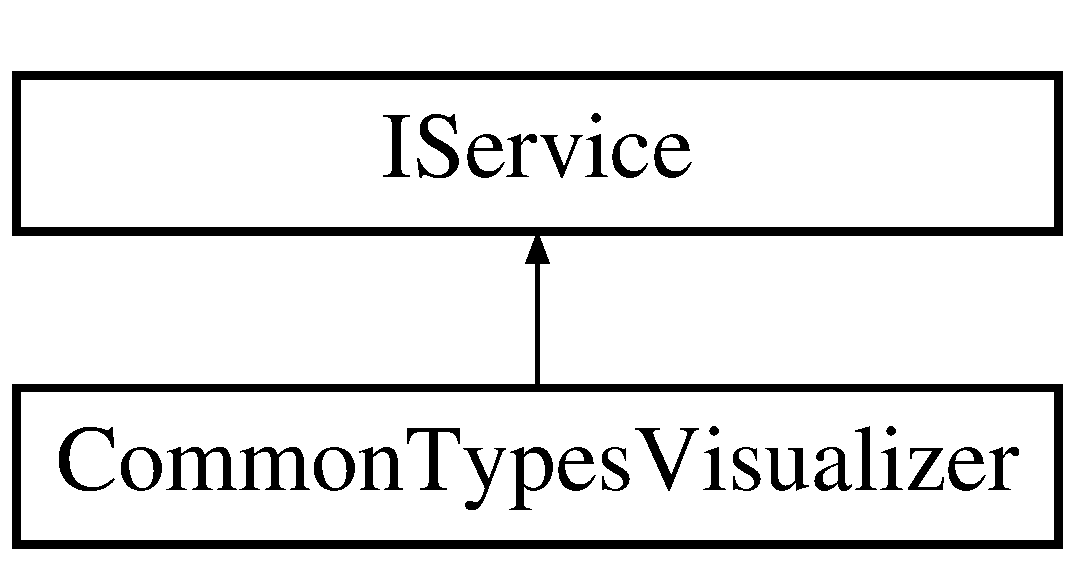
\includegraphics[height=2.000000cm]{classCommonTypesVisualizer}
\end{center}
\end{figure}
\subsection*{Public Member Functions}
\begin{DoxyCompactItemize}
\item 
{\bfseries Common\+Types\+Visualizer} (\hyperlink{classPythonModule}{Python\+Module} \&python)\hypertarget{classCommonTypesVisualizer_a30da44a28c61f4b5cb1549bc95ac1d0a}{}\label{classCommonTypesVisualizer_a30da44a28c61f4b5cb1549bc95ac1d0a}

\item 
void {\bfseries On\+Start} () override\hypertarget{classCommonTypesVisualizer_ac6f33a59769e00936e783f1a44f6c364}{}\label{classCommonTypesVisualizer_ac6f33a59769e00936e783f1a44f6c364}

\end{DoxyCompactItemize}


The documentation for this class was generated from the following file\+:\begin{DoxyCompactItemize}
\item 
src/\+Model/python/Common\+Types\+Visualizer.\+h\end{DoxyCompactItemize}

\hypertarget{classComponent}{}\section{Component Class Reference}
\label{classComponent}\index{Component@{Component}}
Inheritance diagram for Component\+:\begin{figure}[H]
\begin{center}
\leavevmode
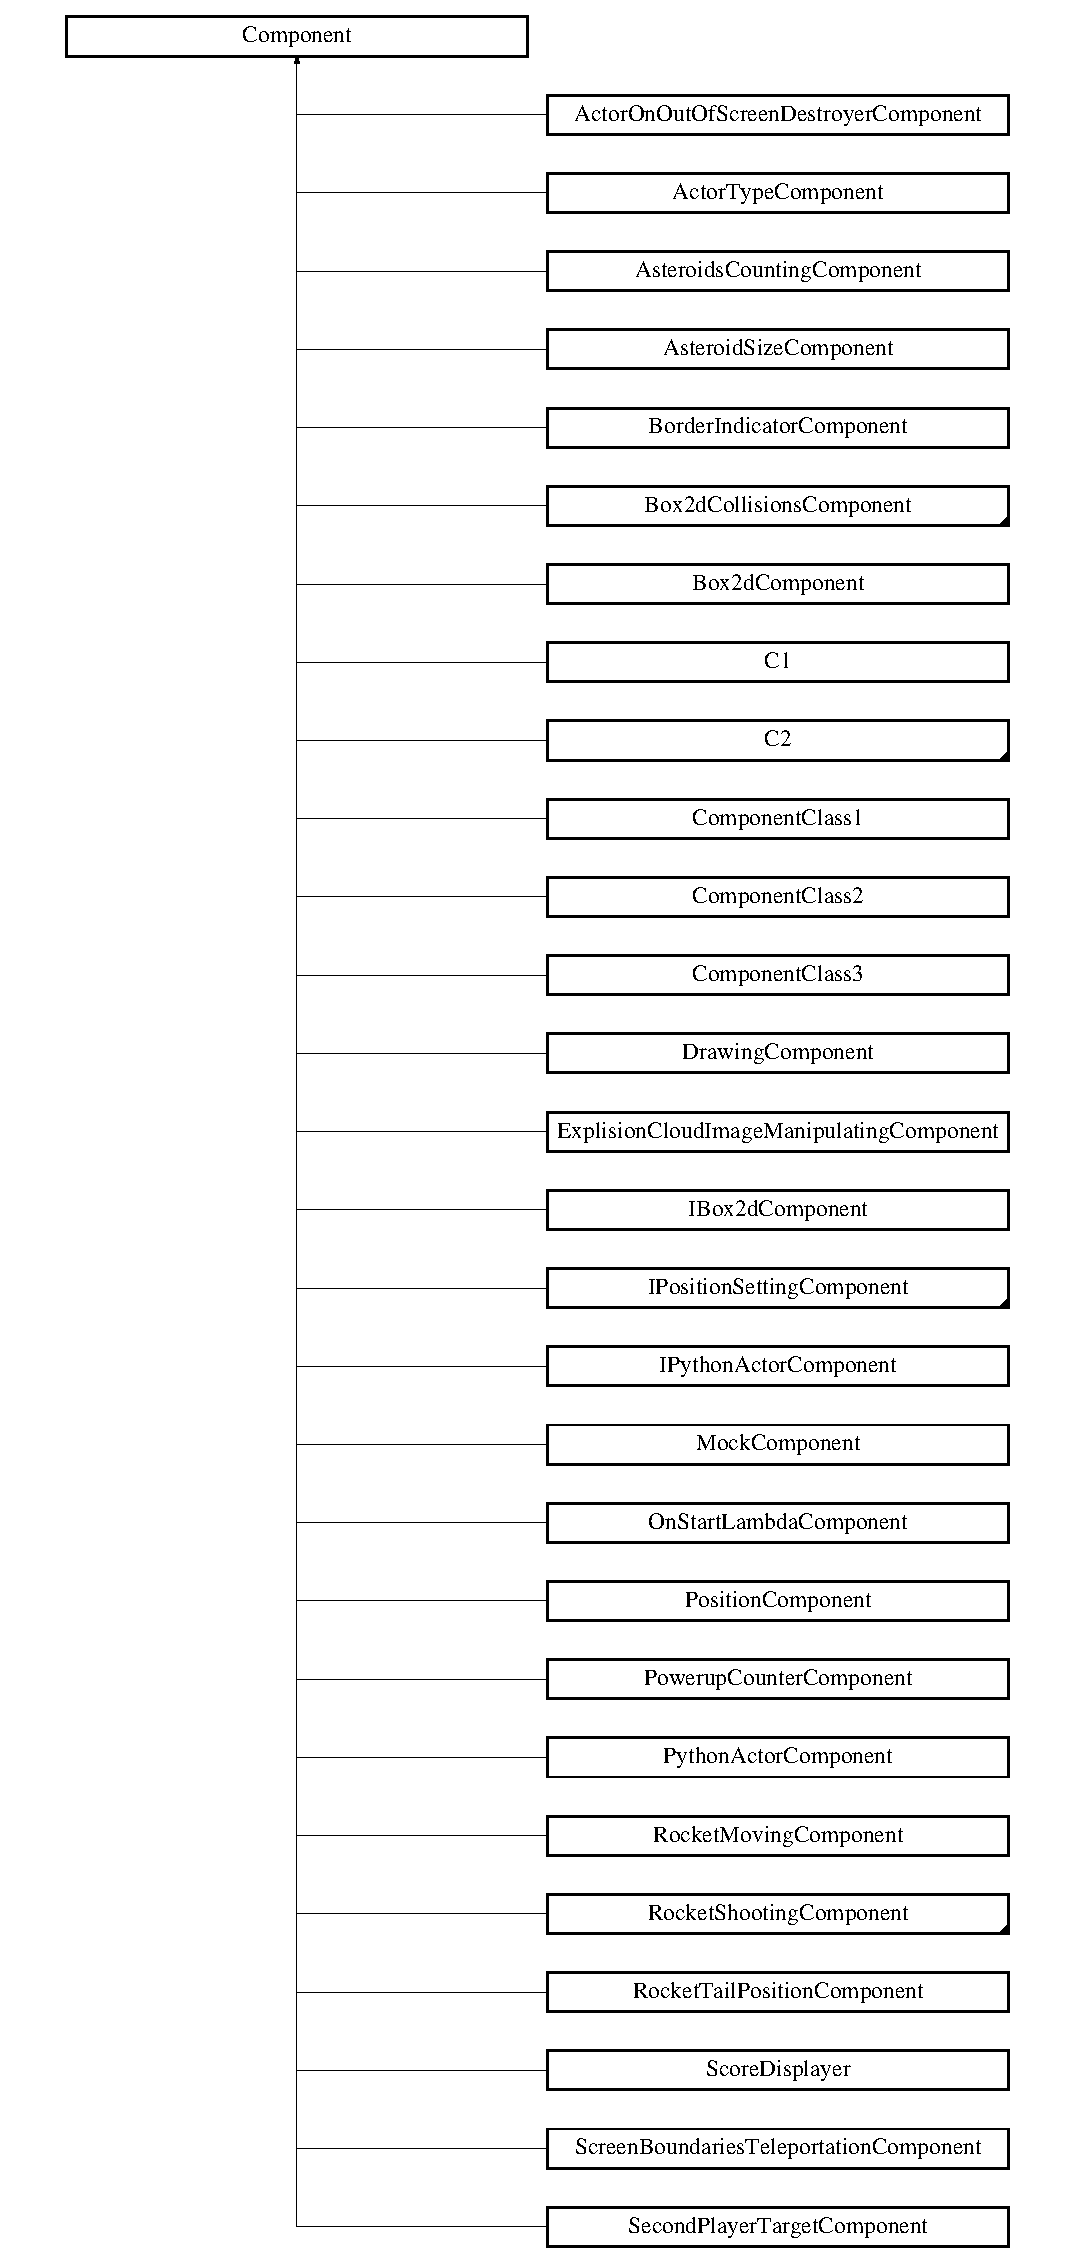
\includegraphics[height=12.000000cm]{classComponent}
\end{center}
\end{figure}
\subsection*{Public Member Functions}
\begin{DoxyCompactItemize}
\item 
virtual void {\bfseries On\+Start} (\hyperlink{classIActor}{I\+Actor} \&actor)\hypertarget{classComponent_ac75891ad8b5dac47d4cec7c0f56c74c9}{}\label{classComponent_ac75891ad8b5dac47d4cec7c0f56c74c9}

\item 
virtual void {\bfseries On\+Update} ()\hypertarget{classComponent_a9680b491a1f64d8d7c140bb526176c74}{}\label{classComponent_a9680b491a1f64d8d7c140bb526176c74}

\item 
virtual void {\bfseries On\+Stop} ()\hypertarget{classComponent_a19dd4b600d60aeddaa41a1fea7e446f4}{}\label{classComponent_a19dd4b600d60aeddaa41a1fea7e446f4}

\end{DoxyCompactItemize}


The documentation for this class was generated from the following files\+:\begin{DoxyCompactItemize}
\item 
src/\+Model/components/Component.\+h\item 
src/\+Model/components/Component.\+cpp\end{DoxyCompactItemize}

\hypertarget{classComponentClass1}{}\section{Component\+Class1 Class Reference}
\label{classComponentClass1}\index{Component\+Class1@{Component\+Class1}}
Inheritance diagram for Component\+Class1\+:\begin{figure}[H]
\begin{center}
\leavevmode
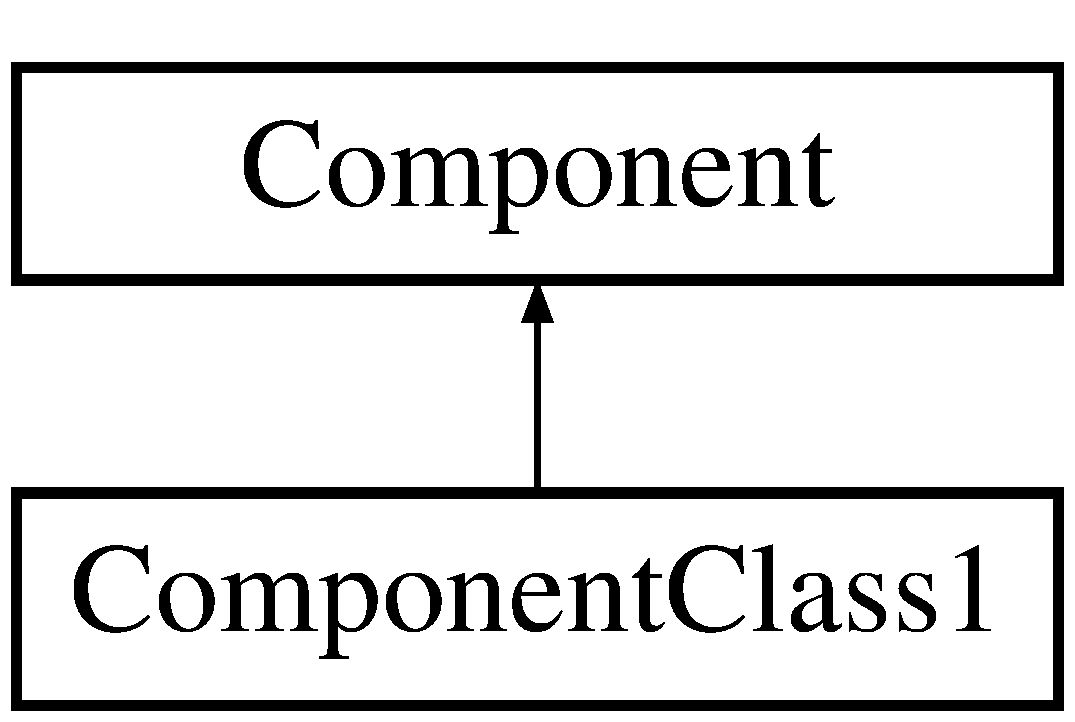
\includegraphics[height=2.000000cm]{classComponentClass1}
\end{center}
\end{figure}
\subsection*{Additional Inherited Members}


The documentation for this class was generated from the following file\+:\begin{DoxyCompactItemize}
\item 
test/Components\+Container\+Test.\+cpp\end{DoxyCompactItemize}

\hypertarget{classComponentClass2}{}\section{Component\+Class2 Class Reference}
\label{classComponentClass2}\index{Component\+Class2@{Component\+Class2}}
Inheritance diagram for Component\+Class2\+:\begin{figure}[H]
\begin{center}
\leavevmode
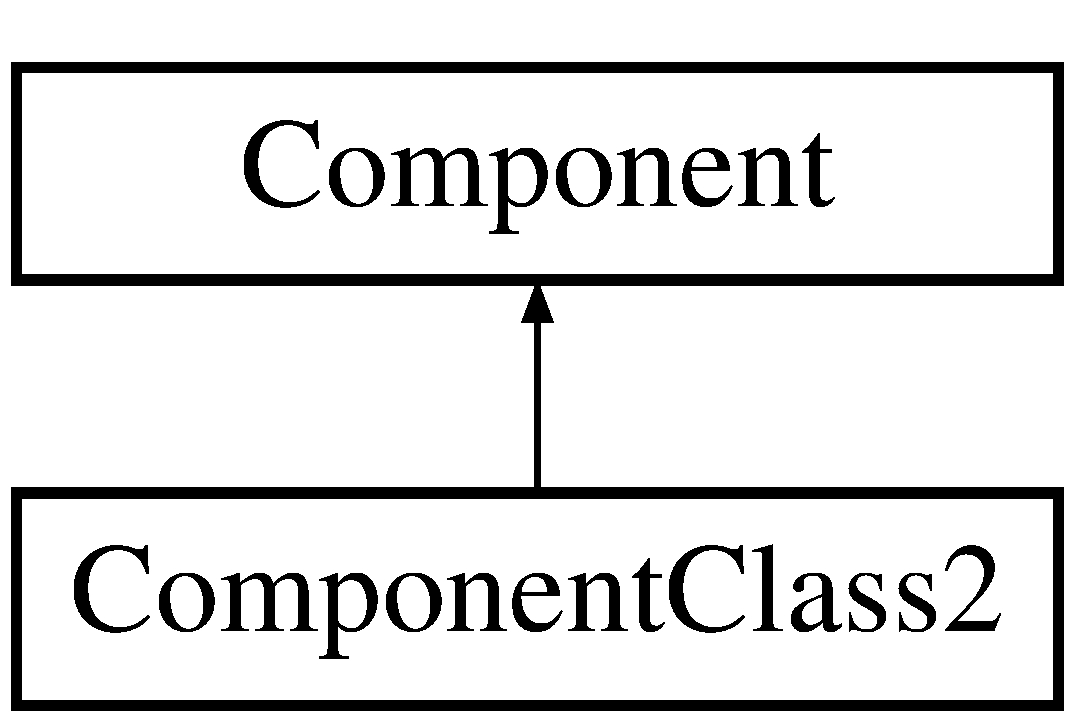
\includegraphics[height=2.000000cm]{classComponentClass2}
\end{center}
\end{figure}
\subsection*{Additional Inherited Members}


The documentation for this class was generated from the following file\+:\begin{DoxyCompactItemize}
\item 
test/Components\+Container\+Test.\+cpp\end{DoxyCompactItemize}

\hypertarget{classComponentClass3}{}\section{Component\+Class3 Class Reference}
\label{classComponentClass3}\index{Component\+Class3@{Component\+Class3}}
Inheritance diagram for Component\+Class3\+:\begin{figure}[H]
\begin{center}
\leavevmode
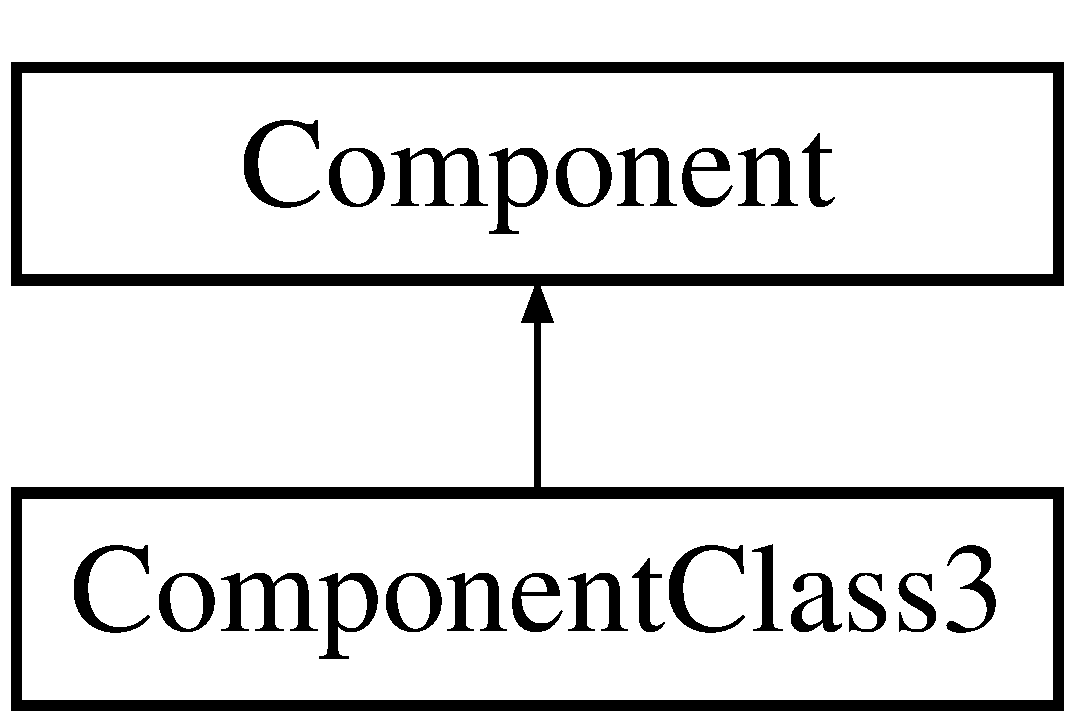
\includegraphics[height=2.000000cm]{classComponentClass3}
\end{center}
\end{figure}
\subsection*{Additional Inherited Members}


The documentation for this class was generated from the following file\+:\begin{DoxyCompactItemize}
\item 
test/Components\+Container\+Test.\+cpp\end{DoxyCompactItemize}

\hypertarget{classComponentsContainer}{}\section{Components\+Container Class Reference}
\label{classComponentsContainer}\index{Components\+Container@{Components\+Container}}
\subsection*{Public Member Functions}
\begin{DoxyCompactItemize}
\item 
void {\bfseries add\+Component} (std\+::shared\+\_\+ptr$<$ \hyperlink{classComponent}{Component} $>$ new\+Component)\hypertarget{classComponentsContainer_a1d0e9c6769a9ab7245a193670cb60433}{}\label{classComponentsContainer_a1d0e9c6769a9ab7245a193670cb60433}

\item 
{\footnotesize template$<$typename Component\+Type $>$ }\\std\+::vector$<$ std\+::shared\+\_\+ptr$<$ Component\+Type $>$ $>$ {\bfseries get\+Components} ()\hypertarget{classComponentsContainer_a343f4ce6a7b5660522d0443f2a731359}{}\label{classComponentsContainer_a343f4ce6a7b5660522d0443f2a731359}

\item 
std\+::vector$<$ std\+::shared\+\_\+ptr$<$ \hyperlink{classComponent}{Component} $>$ $>$ {\bfseries get\+Components} (\hyperlink{classComponentTypeChecker}{Component\+Type\+Checker} checker)\hypertarget{classComponentsContainer_a65a03d86c1acd71561ac0e97d02c69be}{}\label{classComponentsContainer_a65a03d86c1acd71561ac0e97d02c69be}

\item 
std\+::vector$<$ std\+::shared\+\_\+ptr$<$ \hyperlink{classComponent}{Component} $>$ $>$ {\bfseries get\+All\+Components} ()\hypertarget{classComponentsContainer_a037964e3642fbf43a1f48bd2a8ed66af}{}\label{classComponentsContainer_a037964e3642fbf43a1f48bd2a8ed66af}

\item 
std\+::shared\+\_\+ptr$<$ \hyperlink{classComponent}{Component} $>$ {\bfseries get\+Only\+Component} (\hyperlink{classComponentTypeChecker}{Component\+Type\+Checker} checker)\hypertarget{classComponentsContainer_a706b6e740715baf62254a1ad22d35f73}{}\label{classComponentsContainer_a706b6e740715baf62254a1ad22d35f73}

\item 
bool {\bfseries is\+Component\+Present} (\hyperlink{classComponentTypeChecker}{Component\+Type\+Checker} checker)\hypertarget{classComponentsContainer_ad0b2b7ab32d0e231c63578f537d0875c}{}\label{classComponentsContainer_ad0b2b7ab32d0e231c63578f537d0875c}

\item 
void {\bfseries remove\+Component} (\hyperlink{classComponent}{Component} $\ast$component)\hypertarget{classComponentsContainer_aad6e15f7d4758d36e7a356d31ebe1750}{}\label{classComponentsContainer_aad6e15f7d4758d36e7a356d31ebe1750}

\end{DoxyCompactItemize}


The documentation for this class was generated from the following files\+:\begin{DoxyCompactItemize}
\item 
src/\+Model/components/Components\+Container.\+h\item 
src/\+Model/components/Components\+Container.\+cpp\end{DoxyCompactItemize}

\hypertarget{classComponentsContainerTest}{}\section{Components\+Container\+Test Class Reference}
\label{classComponentsContainerTest}\index{Components\+Container\+Test@{Components\+Container\+Test}}
Inheritance diagram for Components\+Container\+Test\+:\begin{figure}[H]
\begin{center}
\leavevmode
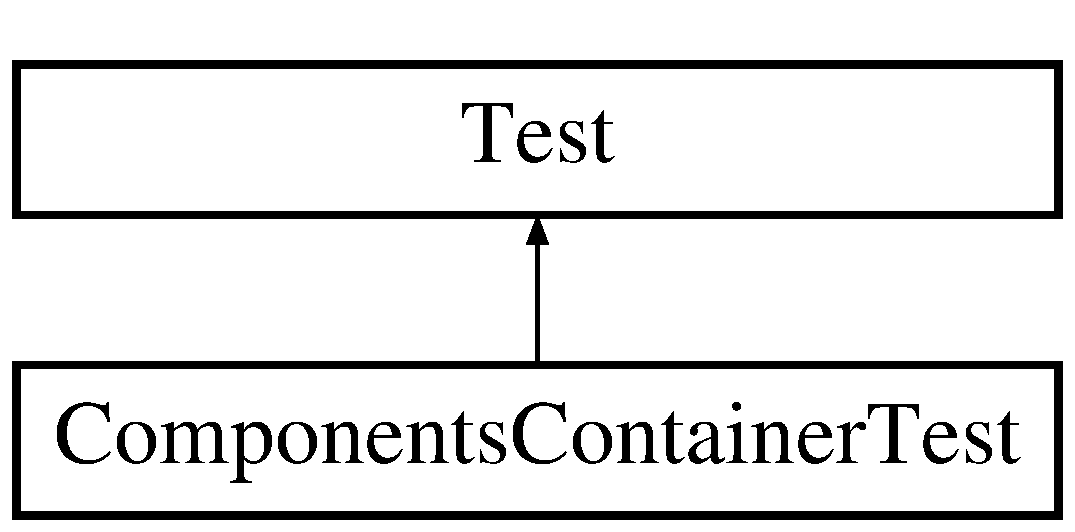
\includegraphics[height=2.000000cm]{classComponentsContainerTest}
\end{center}
\end{figure}
\subsection*{Public Member Functions}
\begin{DoxyCompactItemize}
\item 
{\footnotesize template$<$typename T $>$ }\\void {\bfseries add\+Components} (std\+::vector$<$ T $>$ vector)\hypertarget{classComponentsContainerTest_a93cb48e1a34f76c17a42f332e09c1ce1}{}\label{classComponentsContainerTest_a93cb48e1a34f76c17a42f332e09c1ce1}

\item 
{\footnotesize template$<$typename T1 , typename T2 $>$ }\\void {\bfseries assert\+Contains\+Components} (std\+::vector$<$ T1 $>$ vector\+To\+Be\+Looking\+Into, std\+::vector$<$ T2 $>$ elements\+We\+Are\+Searching)\hypertarget{classComponentsContainerTest_a50cef55afdfa4ead49156f6b2936c15c}{}\label{classComponentsContainerTest_a50cef55afdfa4ead49156f6b2936c15c}

\end{DoxyCompactItemize}
\subsection*{Public Attributes}
\begin{DoxyCompactItemize}
\item 
\hyperlink{classComponentsContainer}{Components\+Container} {\bfseries container}\hypertarget{classComponentsContainerTest_a28409e522854cb2dc8960c6a95251f78}{}\label{classComponentsContainerTest_a28409e522854cb2dc8960c6a95251f78}

\end{DoxyCompactItemize}


The documentation for this class was generated from the following file\+:\begin{DoxyCompactItemize}
\item 
test/Components\+Container\+Test.\+cpp\end{DoxyCompactItemize}

\hypertarget{classComponentTypeChecker}{}\section{Component\+Type\+Checker Class Reference}
\label{classComponentTypeChecker}\index{Component\+Type\+Checker@{Component\+Type\+Checker}}
\subsection*{Public Member Functions}
\begin{DoxyCompactItemize}
\item 
{\footnotesize template$<$typename Component\+Type $>$ }\\{\bfseries Component\+Type\+Checker} (Component\+Type $\ast$)\hypertarget{classComponentTypeChecker_adb04cf1c48a7e335146addc072fba1f9}{}\label{classComponentTypeChecker_adb04cf1c48a7e335146addc072fba1f9}

\item 
bool {\bfseries was\+Cast\+Succesfull} (\hyperlink{classComponent}{Component} $\ast$component\+We\+Are\+Checking)\hypertarget{classComponentTypeChecker_ae950a7cc04452b3f2a96542febce5eb8}{}\label{classComponentTypeChecker_ae950a7cc04452b3f2a96542febce5eb8}

\end{DoxyCompactItemize}
\subsection*{Static Public Member Functions}
\begin{DoxyCompactItemize}
\item 
{\footnotesize template$<$typename Component\+Type $>$ }\\static \hyperlink{classComponentTypeChecker}{Component\+Type\+Checker} {\bfseries create} ()\hypertarget{classComponentTypeChecker_ae96c2f4ba47734b47b2735c18696be44}{}\label{classComponentTypeChecker_ae96c2f4ba47734b47b2735c18696be44}

\end{DoxyCompactItemize}


The documentation for this class was generated from the following file\+:\begin{DoxyCompactItemize}
\item 
src/\+Model/components/Component\+Type\+Checker.\+h\end{DoxyCompactItemize}

\hypertarget{classConsoleScreen}{}\section{Console\+Screen Class Reference}
\label{classConsoleScreen}\index{Console\+Screen@{Console\+Screen}}
Inheritance diagram for Console\+Screen\+:\begin{figure}[H]
\begin{center}
\leavevmode
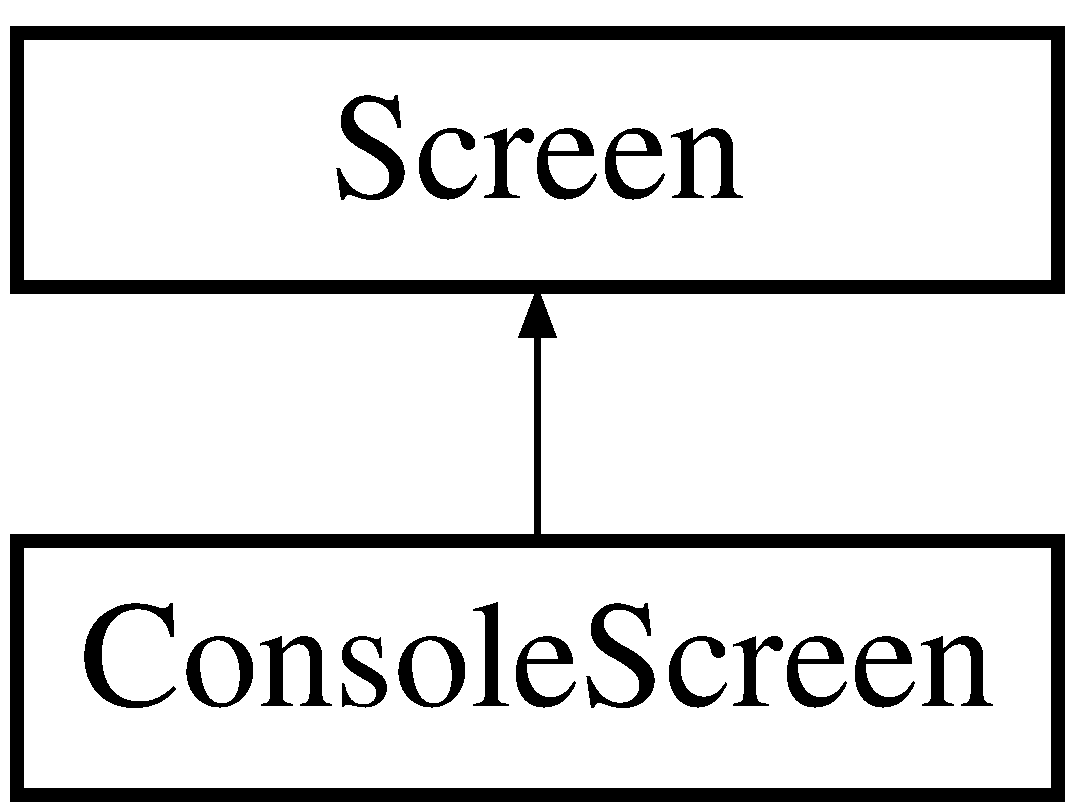
\includegraphics[height=2.000000cm]{classConsoleScreen}
\end{center}
\end{figure}
\subsection*{Public Member Functions}
\begin{DoxyCompactItemize}
\item 
void \hyperlink{classConsoleScreen_a6db8562435775c00363479c303d884a5}{event\+Action} (A\+L\+L\+E\+G\+R\+O\+\_\+\+E\+V\+E\+NT \&, \hyperlink{classViewManager}{View\+Manager} $\ast$, \hyperlink{classGame}{Game} $\ast$)
\item 
void \hyperlink{classConsoleScreen_a512a1401ec957d5d2d504aafd315362d}{update\+Screen\+After\+Display\+Changes} ()
\item 
void \hyperlink{classConsoleScreen_a632e8a9ebefb9574537d5268e6ae805f}{initialize\+Screen\+Elements} ()
\item 
std\+::string \hyperlink{classConsoleScreen_a826d101fdea392e61d6d4f5b1087a33f}{get\+Title} ()
\item 
void {\bfseries update\+Screen} ()\hypertarget{classConsoleScreen_a0439f4f690a398f43952a6dffb7b2b20}{}\label{classConsoleScreen_a0439f4f690a398f43952a6dffb7b2b20}

\item 
{\bfseries Console\+Screen} (std\+::string, \hyperlink{classDisplay}{Display} $\ast$display)\hypertarget{classConsoleScreen_a01b953aaa725a0b844d530b0f6d042bf}{}\label{classConsoleScreen_a01b953aaa725a0b844d530b0f6d042bf}

\item 
void {\bfseries add\+Character} (int character)\hypertarget{classConsoleScreen_a53358e8bf5f4dbacd719e993644335c8}{}\label{classConsoleScreen_a53358e8bf5f4dbacd719e993644335c8}

\item 
void {\bfseries remove\+Screenshot} ()\hypertarget{classConsoleScreen_afc261c0c2a8945de896c46e314f8988c}{}\label{classConsoleScreen_afc261c0c2a8945de896c46e314f8988c}

\item 
void {\bfseries remove\+Character} ()\hypertarget{classConsoleScreen_a3030f2a5ba1a99cf3c1bcdd1db06b943}{}\label{classConsoleScreen_a3030f2a5ba1a99cf3c1bcdd1db06b943}

\item 
std\+::string {\bfseries get\+Last\+Line} ()\hypertarget{classConsoleScreen_a70051b4511a76d81ba6483128a6d9658}{}\label{classConsoleScreen_a70051b4511a76d81ba6483128a6d9658}

\item 
void {\bfseries add\+New\+Line} ()\hypertarget{classConsoleScreen_a69265f0111b9fd6c0f0e65fbe0f70771}{}\label{classConsoleScreen_a69265f0111b9fd6c0f0e65fbe0f70771}

\item 
bool {\bfseries is\+Screenshot\+Taken} ()\hypertarget{classConsoleScreen_ad7bc53aee06514062a6c72e31e00ec1a}{}\label{classConsoleScreen_ad7bc53aee06514062a6c72e31e00ec1a}

\item 
void {\bfseries take\+Screenshot} ()\hypertarget{classConsoleScreen_af6b9e6d03d28cdad8031351efda023bb}{}\label{classConsoleScreen_af6b9e6d03d28cdad8031351efda023bb}

\item 
void {\bfseries write\+Text} (std\+::string line)\hypertarget{classConsoleScreen_ad58f19afabec8d5cbc23e88aa775b518}{}\label{classConsoleScreen_ad58f19afabec8d5cbc23e88aa775b518}

\end{DoxyCompactItemize}


\subsection{Member Function Documentation}
\index{Console\+Screen@{Console\+Screen}!event\+Action@{event\+Action}}
\index{event\+Action@{event\+Action}!Console\+Screen@{Console\+Screen}}
\subsubsection[{\texorpdfstring{event\+Action(\+A\+L\+L\+E\+G\+R\+O\+\_\+\+E\+V\+E\+N\+T \&, View\+Manager $\ast$, Game $\ast$)}{eventAction(ALLEGRO_EVENT &, ViewManager *, Game *)}}]{\setlength{\rightskip}{0pt plus 5cm}void Console\+Screen\+::event\+Action (
\begin{DoxyParamCaption}
\item[{A\+L\+L\+E\+G\+R\+O\+\_\+\+E\+V\+E\+NT \&}]{ev, }
\item[{{\bf View\+Manager} $\ast$}]{vm, }
\item[{{\bf Game} $\ast$}]{g}
\end{DoxyParamCaption}
)\hspace{0.3cm}{\ttfamily [virtual]}}\hypertarget{classConsoleScreen_a6db8562435775c00363479c303d884a5}{}\label{classConsoleScreen_a6db8562435775c00363479c303d884a5}
Virtual method which does some actions when event occurs. 
\begin{DoxyParams}{Parameters}
{\em ev} & event which occured. \\
\hline
{\em vm} & pointer to the \hyperlink{classViewManager}{View\+Manager}. \\
\hline
{\em g} & pointer to the \hyperlink{classGame}{Game}. \\
\hline
\end{DoxyParams}


Reimplemented from \hyperlink{classScreen_a5fb59d03053c2d0aaca26f9480bbe433}{Screen}.

\index{Console\+Screen@{Console\+Screen}!get\+Title@{get\+Title}}
\index{get\+Title@{get\+Title}!Console\+Screen@{Console\+Screen}}
\subsubsection[{\texorpdfstring{get\+Title()}{getTitle()}}]{\setlength{\rightskip}{0pt plus 5cm}std\+::string Console\+Screen\+::get\+Title (
\begin{DoxyParamCaption}
{}
\end{DoxyParamCaption}
)\hspace{0.3cm}{\ttfamily [inline]}, {\ttfamily [virtual]}}\hypertarget{classConsoleScreen_a826d101fdea392e61d6d4f5b1087a33f}{}\label{classConsoleScreen_a826d101fdea392e61d6d4f5b1087a33f}
Returns \hyperlink{classScreen}{Screen} title (\hyperlink{classScreen}{Screen} titles are used to organize Screens). \begin{DoxyReturn}{Returns}
title of the screen. 
\end{DoxyReturn}


Reimplemented from \hyperlink{classScreen_a28df2a95a64693e2e5b1238c07c92115}{Screen}.

\index{Console\+Screen@{Console\+Screen}!initialize\+Screen\+Elements@{initialize\+Screen\+Elements}}
\index{initialize\+Screen\+Elements@{initialize\+Screen\+Elements}!Console\+Screen@{Console\+Screen}}
\subsubsection[{\texorpdfstring{initialize\+Screen\+Elements()}{initializeScreenElements()}}]{\setlength{\rightskip}{0pt plus 5cm}void Console\+Screen\+::initialize\+Screen\+Elements (
\begin{DoxyParamCaption}
{}
\end{DoxyParamCaption}
)\hspace{0.3cm}{\ttfamily [virtual]}}\hypertarget{classConsoleScreen_a632e8a9ebefb9574537d5268e6ae805f}{}\label{classConsoleScreen_a632e8a9ebefb9574537d5268e6ae805f}
Virtual method which is used to initialize special elements added to the \hyperlink{classScreen}{Screen} before it will be used 

Reimplemented from \hyperlink{classScreen_a207320477f0e323dc4cd36dbd4706238}{Screen}.

\index{Console\+Screen@{Console\+Screen}!update\+Screen\+After\+Display\+Changes@{update\+Screen\+After\+Display\+Changes}}
\index{update\+Screen\+After\+Display\+Changes@{update\+Screen\+After\+Display\+Changes}!Console\+Screen@{Console\+Screen}}
\subsubsection[{\texorpdfstring{update\+Screen\+After\+Display\+Changes()}{updateScreenAfterDisplayChanges()}}]{\setlength{\rightskip}{0pt plus 5cm}void Console\+Screen\+::update\+Screen\+After\+Display\+Changes (
\begin{DoxyParamCaption}
{}
\end{DoxyParamCaption}
)\hspace{0.3cm}{\ttfamily [virtual]}}\hypertarget{classConsoleScreen_a512a1401ec957d5d2d504aafd315362d}{}\label{classConsoleScreen_a512a1401ec957d5d2d504aafd315362d}
Let\textquotesingle{}s the \hyperlink{classScreen}{Screen} to change it\textquotesingle{}s objects after changes in the display (like resolution). 

Reimplemented from \hyperlink{classScreen_a0d283acd7432bd4fedd35cd147bdf4a8}{Screen}.



The documentation for this class was generated from the following files\+:\begin{DoxyCompactItemize}
\item 
src/\+View/Console\+Screen.\+h\item 
src/\+View/Console\+Screen.\+cpp\end{DoxyCompactItemize}

\hypertarget{classConsoleScreenEventInterpreter}{}\section{Console\+Screen\+Event\+Interpreter Class Reference}
\label{classConsoleScreenEventInterpreter}\index{Console\+Screen\+Event\+Interpreter@{Console\+Screen\+Event\+Interpreter}}
Inheritance diagram for Console\+Screen\+Event\+Interpreter\+:\begin{figure}[H]
\begin{center}
\leavevmode
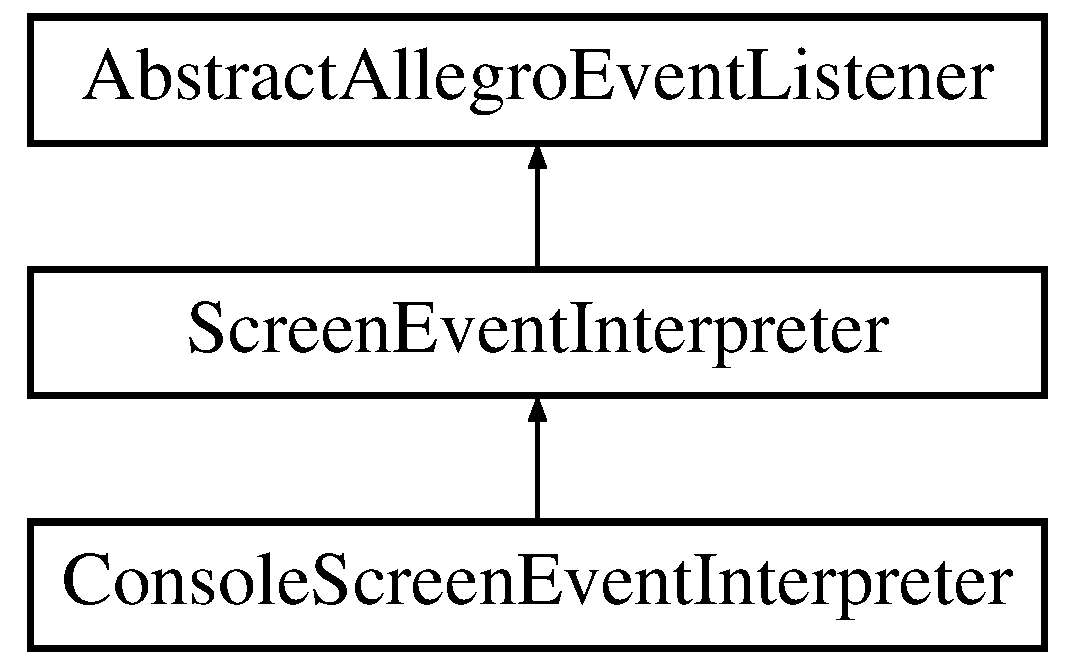
\includegraphics[height=3.000000cm]{classConsoleScreenEventInterpreter}
\end{center}
\end{figure}
\subsection*{Public Member Functions}
\begin{DoxyCompactItemize}
\item 
{\bfseries Console\+Screen\+Event\+Interpreter} (\hyperlink{classConsoleScreen}{Console\+Screen} $\ast$console\+Screen, \hyperlink{classGame}{Game} \&game)\hypertarget{classConsoleScreenEventInterpreter_a16532522d008b711ed848320a757fdfa}{}\label{classConsoleScreenEventInterpreter_a16532522d008b711ed848320a757fdfa}

\item 
virtual void {\bfseries key\+Down} (int keynum)\hypertarget{classConsoleScreenEventInterpreter_aec30e5200c0ed4f8983a457f85e5643b}{}\label{classConsoleScreenEventInterpreter_aec30e5200c0ed4f8983a457f85e5643b}

\item 
virtual void {\bfseries char\+Key\+Down} (int unicode)\hypertarget{classConsoleScreenEventInterpreter_ab55a2e02c5a3ed8e7b7ad4ececc04f9e}{}\label{classConsoleScreenEventInterpreter_ab55a2e02c5a3ed8e7b7ad4ececc04f9e}

\item 
virtual void {\bfseries time\+Event} ()\hypertarget{classConsoleScreenEventInterpreter_a74c757a9c88027df958af48945345248}{}\label{classConsoleScreenEventInterpreter_a74c757a9c88027df958af48945345248}

\item 
virtual std\+::string {\bfseries get\+Screen\+Name} ()\hypertarget{classConsoleScreenEventInterpreter_acba5aab5a9c627e47f636cb6d58645c5}{}\label{classConsoleScreenEventInterpreter_acba5aab5a9c627e47f636cb6d58645c5}

\end{DoxyCompactItemize}
\subsection*{Additional Inherited Members}


The documentation for this class was generated from the following files\+:\begin{DoxyCompactItemize}
\item 
src/\+Controller/Console\+Screen\+Event\+Interpreter.\+h\item 
src/\+Controller/Console\+Screen\+Event\+Interpreter.\+cpp\end{DoxyCompactItemize}

\hypertarget{classContactComponentsContainer}{}\section{Contact\+Components\+Container Class Reference}
\label{classContactComponentsContainer}\index{Contact\+Components\+Container@{Contact\+Components\+Container}}
\subsection*{Public Member Functions}
\begin{DoxyCompactItemize}
\item 
\hyperlink{classBox2dCollisionsComponent}{Box2d\+Collisions\+Component} $\ast$ {\bfseries get\+Component\+For\+Body} (b2\+Body $\ast$body)\hypertarget{classContactComponentsContainer_ac17b948c7e104ce75f20795e63fe4194}{}\label{classContactComponentsContainer_ac17b948c7e104ce75f20795e63fe4194}

\item 
void {\bfseries register\+Collision\+Component} (b2\+Body $\ast$body, \hyperlink{classBox2dCollisionsComponent}{Box2d\+Collisions\+Component} $\ast$component)\hypertarget{classContactComponentsContainer_af64b4fb5377ba04e336de1c88231209b}{}\label{classContactComponentsContainer_af64b4fb5377ba04e336de1c88231209b}

\item 
void {\bfseries deregister\+Collision\+Component} (b2\+Body $\ast$body)\hypertarget{classContactComponentsContainer_a2aff9381caf7154d8a301dc43d3feee4}{}\label{classContactComponentsContainer_a2aff9381caf7154d8a301dc43d3feee4}

\end{DoxyCompactItemize}


The documentation for this class was generated from the following files\+:\begin{DoxyCompactItemize}
\item 
src/\+Model/collisions/Contact\+Components\+Container.\+h\item 
src/\+Model/collisions/Contact\+Components\+Container.\+cpp\end{DoxyCompactItemize}

\hypertarget{classDegreesCalculations}{}\section{Degrees\+Calculations Class Reference}
\label{classDegreesCalculations}\index{Degrees\+Calculations@{Degrees\+Calculations}}
\subsection*{Static Public Member Functions}
\begin{DoxyCompactItemize}
\item 
static \hyperlink{classRotation}{Rotation} {\bfseries radians\+To\+Degrees} (double rad)\hypertarget{classDegreesCalculations_a94ae980258188bfe2d234038764c016f}{}\label{classDegreesCalculations_a94ae980258188bfe2d234038764c016f}

\item 
static double {\bfseries degrees\+To\+Radians} (\hyperlink{classRotation}{Rotation} degrees)\hypertarget{classDegreesCalculations_ace75036176cddf90162bafc2746d6611}{}\label{classDegreesCalculations_ace75036176cddf90162bafc2746d6611}

\end{DoxyCompactItemize}


The documentation for this class was generated from the following files\+:\begin{DoxyCompactItemize}
\item 
src/\+Model/help/Degrees\+Calculations.\+h\item 
src/\+Model/help/Degrees\+Calculations.\+cpp\end{DoxyCompactItemize}

\hypertarget{classDisplay}{}\section{Display Class Reference}
\label{classDisplay}\index{Display@{Display}}


{\ttfamily \#include $<$Display.\+h$>$}

\subsection*{Public Member Functions}
\begin{DoxyCompactItemize}
\item 
void \hyperlink{classDisplay_ad735068ee75f69ff87373dc80607a6de}{draw\+Scene\+On\+Display} (\hyperlink{classScene}{Scene} $\ast$)
\item 
void \hyperlink{classDisplay_af4cf5b66237916d8c4b1baf135037202}{clear\+Display} (int, int, int)
\item 
void \hyperlink{classDisplay_a6de73ad4135258995b2deee44e1e628a}{resize\+Display} (int, int)
\item 
void {\bfseries flip\+Display} ()\hypertarget{classDisplay_a9b945675bac2549db7a392c9ef242ee5}{}\label{classDisplay_a9b945675bac2549db7a392c9ef242ee5}

\item 
A\+L\+L\+E\+G\+R\+O\+\_\+\+D\+I\+S\+P\+L\+AY $\ast$ {\bfseries get\+Display} ()\hypertarget{classDisplay_a6ea827abdef4bc9496d565296c9da61e}{}\label{classDisplay_a6ea827abdef4bc9496d565296c9da61e}

\item 
{\bfseries Display} (int=640, int=480)\hypertarget{classDisplay_ac962d82df123871e4bdc6cae9c9613e7}{}\label{classDisplay_ac962d82df123871e4bdc6cae9c9613e7}

\end{DoxyCompactItemize}


\subsection{Detailed Description}
Class whoch organizes A\+L\+L\+E\+G\+R\+O\+\_\+\+D\+I\+S\+P\+L\+AY. 

\subsection{Member Function Documentation}
\index{Display@{Display}!clear\+Display@{clear\+Display}}
\index{clear\+Display@{clear\+Display}!Display@{Display}}
\subsubsection[{\texorpdfstring{clear\+Display(int, int, int)}{clearDisplay(int, int, int)}}]{\setlength{\rightskip}{0pt plus 5cm}void Display\+::clear\+Display (
\begin{DoxyParamCaption}
\item[{int}]{r, }
\item[{int}]{g, }
\item[{int}]{b}
\end{DoxyParamCaption}
)}\hypertarget{classDisplay_af4cf5b66237916d8c4b1baf135037202}{}\label{classDisplay_af4cf5b66237916d8c4b1baf135037202}
Clears \hyperlink{classDisplay}{Display} for the given color in R\+GB palette. 
\begin{DoxyParams}{Parameters}
{\em R} & color \\
\hline
{\em G} & color \\
\hline
{\em B} & color \\
\hline
\end{DoxyParams}
\index{Display@{Display}!draw\+Scene\+On\+Display@{draw\+Scene\+On\+Display}}
\index{draw\+Scene\+On\+Display@{draw\+Scene\+On\+Display}!Display@{Display}}
\subsubsection[{\texorpdfstring{draw\+Scene\+On\+Display(\+Scene $\ast$)}{drawSceneOnDisplay(Scene *)}}]{\setlength{\rightskip}{0pt plus 5cm}void Display\+::draw\+Scene\+On\+Display (
\begin{DoxyParamCaption}
\item[{{\bf Scene} $\ast$}]{scene}
\end{DoxyParamCaption}
)}\hypertarget{classDisplay_ad735068ee75f69ff87373dc80607a6de}{}\label{classDisplay_ad735068ee75f69ff87373dc80607a6de}
Draws given \hyperlink{classScene}{Scene} on \hyperlink{classDisplay}{Display}. 
\begin{DoxyParams}{Parameters}
{\em pointer} & to the \hyperlink{classScene}{Scene}. \\
\hline
\end{DoxyParams}
\index{Display@{Display}!resize\+Display@{resize\+Display}}
\index{resize\+Display@{resize\+Display}!Display@{Display}}
\subsubsection[{\texorpdfstring{resize\+Display(int, int)}{resizeDisplay(int, int)}}]{\setlength{\rightskip}{0pt plus 5cm}void Display\+::resize\+Display (
\begin{DoxyParamCaption}
\item[{int}]{width, }
\item[{int}]{height}
\end{DoxyParamCaption}
)}\hypertarget{classDisplay_a6de73ad4135258995b2deee44e1e628a}{}\label{classDisplay_a6de73ad4135258995b2deee44e1e628a}
Resizes \hyperlink{classDisplay}{Display} for the given dimensions. 
\begin{DoxyParams}{Parameters}
{\em width} & \\
\hline
{\em height} & \\
\hline
\end{DoxyParams}


The documentation for this class was generated from the following files\+:\begin{DoxyCompactItemize}
\item 
src/\+View/Display.\+h\item 
src/\+View/Display.\+cpp\end{DoxyCompactItemize}

\hypertarget{classDrawableObject}{}\section{Drawable\+Object Class Reference}
\label{classDrawableObject}\index{Drawable\+Object@{Drawable\+Object}}


{\ttfamily \#include $<$Drawable\+Object.\+h$>$}

\subsection*{Public Member Functions}
\begin{DoxyCompactItemize}
\item 
A\+L\+L\+E\+G\+R\+O\+\_\+\+B\+I\+T\+M\+AP $\ast$ {\bfseries get\+Bitmap} ()\hypertarget{classDrawableObject_a24589e56097b354e54daff2351ef8646}{}\label{classDrawableObject_a24589e56097b354e54daff2351ef8646}

\item 
void {\bfseries set\+Bitmap} (A\+L\+L\+E\+G\+R\+O\+\_\+\+B\+I\+T\+M\+AP $\ast$new\+Bitmap)\hypertarget{classDrawableObject_af24ffb9aa05616ecfe7a91076e4ef9f1}{}\label{classDrawableObject_af24ffb9aa05616ecfe7a91076e4ef9f1}

\item 
std\+::string {\bfseries get\+Text} ()\hypertarget{classDrawableObject_a10c3b5011225e6336609f7fa1a5081cc}{}\label{classDrawableObject_a10c3b5011225e6336609f7fa1a5081cc}

\item 
void {\bfseries set\+Text} (std\+::string new\+Text)\hypertarget{classDrawableObject_aa1cfa32a445847c11f08e8d730908dee}{}\label{classDrawableObject_aa1cfa32a445847c11f08e8d730908dee}

\item 
bool {\bfseries is\+Text} ()\hypertarget{classDrawableObject_ae635cb4eeca6c33ee243f00004a920a2}{}\label{classDrawableObject_ae635cb4eeca6c33ee243f00004a920a2}

\item 
int {\bfseries get\+PozX} ()\hypertarget{classDrawableObject_af22b9de5fd585984890a84266ffd4e82}{}\label{classDrawableObject_af22b9de5fd585984890a84266ffd4e82}

\item 
void {\bfseries set\+PozX} (int newX)\hypertarget{classDrawableObject_ae7d27907929ab4536882b2a8eed38758}{}\label{classDrawableObject_ae7d27907929ab4536882b2a8eed38758}

\item 
int {\bfseries get\+PozY} ()\hypertarget{classDrawableObject_af777ba956aa537c2010503e7afd9c989}{}\label{classDrawableObject_af777ba956aa537c2010503e7afd9c989}

\item 
void {\bfseries set\+PozY} (int newY)\hypertarget{classDrawableObject_a72e4020e6c644b6f49967919d570a5c3}{}\label{classDrawableObject_a72e4020e6c644b6f49967919d570a5c3}

\item 
float {\bfseries get\+Angle} ()\hypertarget{classDrawableObject_a0b1c1d78462df6eef7a04f7048a01094}{}\label{classDrawableObject_a0b1c1d78462df6eef7a04f7048a01094}

\item 
void {\bfseries set\+Angle} (float new\+Angle)\hypertarget{classDrawableObject_a175745c551dc510cf4a5d12ed292d489}{}\label{classDrawableObject_a175745c551dc510cf4a5d12ed292d489}

\item 
float {\bfseries get\+Zoom} ()\hypertarget{classDrawableObject_ac4ab74d6e8db262f481b9761d36d2809}{}\label{classDrawableObject_ac4ab74d6e8db262f481b9761d36d2809}

\item 
void {\bfseries set\+Zoom} (float new\+Zoom)\hypertarget{classDrawableObject_a21c79eddddb1fba0a3dca0f7ca8b2b24}{}\label{classDrawableObject_a21c79eddddb1fba0a3dca0f7ca8b2b24}

\item 
int {\bfseries get\+TextX} ()\hypertarget{classDrawableObject_ac11c07d032abaf1a0aef0f6516b9c46c}{}\label{classDrawableObject_ac11c07d032abaf1a0aef0f6516b9c46c}

\item 
void {\bfseries set\+TextX} (int new\+TextX)\hypertarget{classDrawableObject_acf99930deee75aaac58621527224d610}{}\label{classDrawableObject_acf99930deee75aaac58621527224d610}

\item 
int {\bfseries get\+TextY} ()\hypertarget{classDrawableObject_a2705ac4ae4d3e3d65ed6aaa4cf37cd82}{}\label{classDrawableObject_a2705ac4ae4d3e3d65ed6aaa4cf37cd82}

\item 
void {\bfseries set\+TextY} (int new\+TextY)\hypertarget{classDrawableObject_ab5f58767df88821fd87fbcc3cacf8de8}{}\label{classDrawableObject_ab5f58767df88821fd87fbcc3cacf8de8}

\item 
int {\bfseries get\+TintR} ()\hypertarget{classDrawableObject_a0b28188501e9a91f6b033ac120ef163b}{}\label{classDrawableObject_a0b28188501e9a91f6b033ac120ef163b}

\item 
void {\bfseries set\+TintR} (int new\+TintR)\hypertarget{classDrawableObject_a63d9ea5b6b13b6467d52898762466494}{}\label{classDrawableObject_a63d9ea5b6b13b6467d52898762466494}

\item 
int {\bfseries get\+TintG} ()\hypertarget{classDrawableObject_a94e7b6e47036ed97b21dd896468783b5}{}\label{classDrawableObject_a94e7b6e47036ed97b21dd896468783b5}

\item 
void {\bfseries set\+TintG} (int new\+TintG)\hypertarget{classDrawableObject_a81a483c62bd4dabef7903e85a88dbff3}{}\label{classDrawableObject_a81a483c62bd4dabef7903e85a88dbff3}

\item 
int {\bfseries get\+TintB} ()\hypertarget{classDrawableObject_aa4edfb17d39895558958c096572ab2ac}{}\label{classDrawableObject_aa4edfb17d39895558958c096572ab2ac}

\item 
void {\bfseries set\+TintB} (int new\+TintB)\hypertarget{classDrawableObject_ae0f50ac01b3d4192abdb5dd89de805a2}{}\label{classDrawableObject_ae0f50ac01b3d4192abdb5dd89de805a2}

\item 
void \hyperlink{classDrawableObject_a173f6a4ac4aa12157cccef15089db4d3}{set\+Tint} (int new\+TintR, int new\+TintG, int new\+TintB)
\item 
{\bfseries Drawable\+Object} (int x, int y, const char $\ast$path=N\+U\+LL, const char $\ast$t=N\+U\+LL, float a=0.\+0f, float z=1.\+0f, int tx=0, int ty=0)\hypertarget{classDrawableObject_adf15c4092f15bd7d42edfc2cdda6cac7}{}\label{classDrawableObject_adf15c4092f15bd7d42edfc2cdda6cac7}

\end{DoxyCompactItemize}


\subsection{Detailed Description}
Basic object which is used to be drawn on \hyperlink{classDisplay}{Display}. 

\subsection{Member Function Documentation}
\index{Drawable\+Object@{Drawable\+Object}!set\+Tint@{set\+Tint}}
\index{set\+Tint@{set\+Tint}!Drawable\+Object@{Drawable\+Object}}
\subsubsection[{\texorpdfstring{set\+Tint(int new\+Tint\+R, int new\+Tint\+G, int new\+Tint\+B)}{setTint(int newTintR, int newTintG, int newTintB)}}]{\setlength{\rightskip}{0pt plus 5cm}void Drawable\+Object\+::set\+Tint (
\begin{DoxyParamCaption}
\item[{int}]{new\+TintR, }
\item[{int}]{new\+TintG, }
\item[{int}]{new\+TintB}
\end{DoxyParamCaption}
)\hspace{0.3cm}{\ttfamily [inline]}}\hypertarget{classDrawableObject_a173f6a4ac4aa12157cccef15089db4d3}{}\label{classDrawableObject_a173f6a4ac4aa12157cccef15089db4d3}
Sets tint arguments -\/ changes in colors of the bitmap. 
\begin{DoxyParams}{Parameters}
{\em tint} & for R color \\
\hline
{\em tint} & for G color \\
\hline
{\em tint} & for B color \\
\hline
\end{DoxyParams}


The documentation for this class was generated from the following files\+:\begin{DoxyCompactItemize}
\item 
src/\+View/Drawable\+Object.\+h\item 
src/\+View/Drawable\+Object.\+cpp\end{DoxyCompactItemize}

\hypertarget{classDrawablePrimitiveVisitor}{}\section{Drawable\+Primitive\+Visitor Class Reference}
\label{classDrawablePrimitiveVisitor}\index{Drawable\+Primitive\+Visitor@{Drawable\+Primitive\+Visitor}}
Inheritance diagram for Drawable\+Primitive\+Visitor\+:\begin{figure}[H]
\begin{center}
\leavevmode
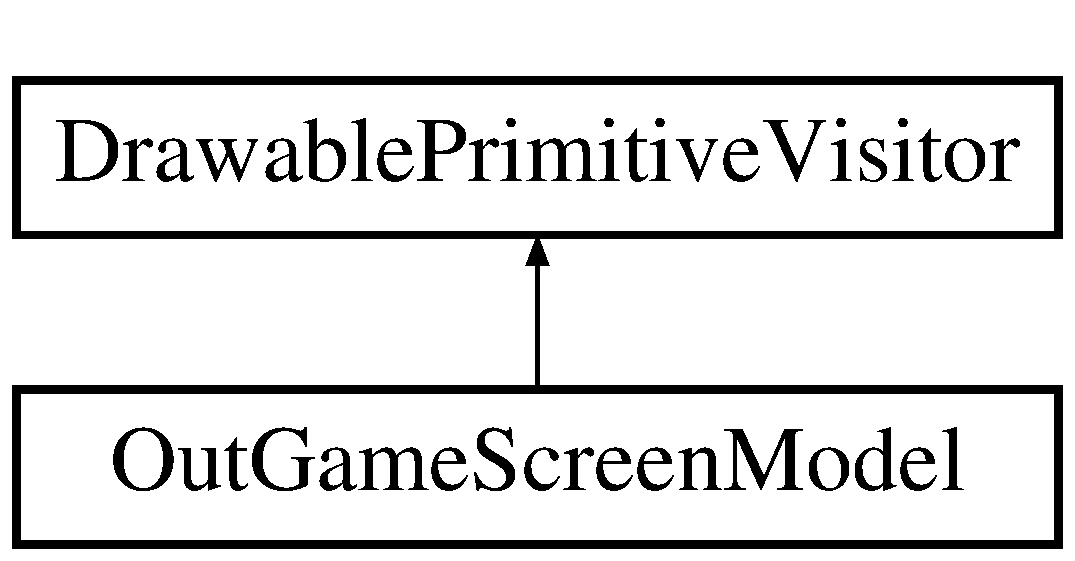
\includegraphics[height=2.000000cm]{classDrawablePrimitiveVisitor}
\end{center}
\end{figure}
\subsection*{Public Member Functions}
\begin{DoxyCompactItemize}
\item 
virtual void {\bfseries visit} (\hyperlink{classImagePrimitive}{Image\+Primitive} \&image)=0\hypertarget{classDrawablePrimitiveVisitor_aeee35001af047b0da48f9e3238487ac1}{}\label{classDrawablePrimitiveVisitor_aeee35001af047b0da48f9e3238487ac1}

\item 
virtual void {\bfseries visit} (\hyperlink{classTextPrimitive}{Text\+Primitive} \&text)=0\hypertarget{classDrawablePrimitiveVisitor_a7c9f6866ddf9bc9cb4968d29bd5cada3}{}\label{classDrawablePrimitiveVisitor_a7c9f6866ddf9bc9cb4968d29bd5cada3}

\end{DoxyCompactItemize}


The documentation for this class was generated from the following file\+:\begin{DoxyCompactItemize}
\item 
src/\+Model/\+Model\+Drawing/Drawable\+Primitive\+Visitor.\+h\end{DoxyCompactItemize}

\hypertarget{classDrawingComponent}{}\section{Drawing\+Component Class Reference}
\label{classDrawingComponent}\index{Drawing\+Component@{Drawing\+Component}}
Inheritance diagram for Drawing\+Component\+:\begin{figure}[H]
\begin{center}
\leavevmode
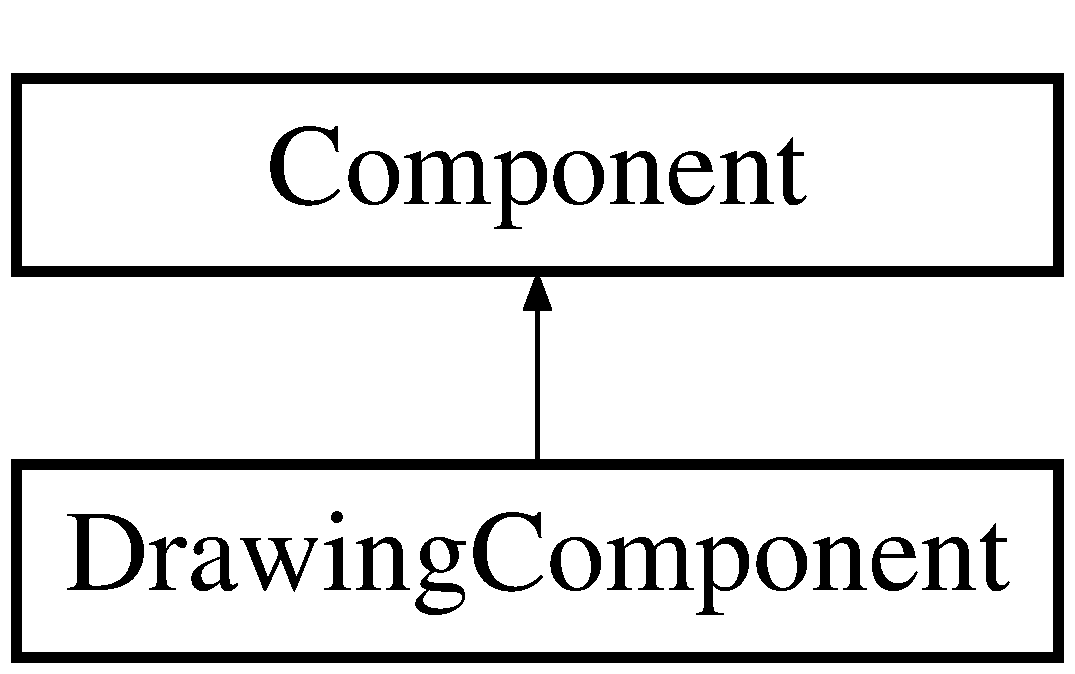
\includegraphics[height=2.000000cm]{classDrawingComponent}
\end{center}
\end{figure}
\subsection*{Public Member Functions}
\begin{DoxyCompactItemize}
\item 
{\bfseries Drawing\+Component} (\hyperlink{classIDrawingSystem}{I\+Drawing\+System} \&drawing\+System, Image\+Primitive\+Type image\+Type, \hyperlink{classScaleToScreen}{Scale\+To\+Screen} scale\+To\+Screen)\hypertarget{classDrawingComponent_a301d028efe8d8184505de81340ccc4a8}{}\label{classDrawingComponent_a301d028efe8d8184505de81340ccc4a8}

\item 
virtual void {\bfseries On\+Start} (\hyperlink{classIActor}{I\+Actor} \&actor)\hypertarget{classDrawingComponent_af7646ccd54c1dd039324d41920b620fe}{}\label{classDrawingComponent_af7646ccd54c1dd039324d41920b620fe}

\item 
virtual void {\bfseries On\+Update} ()\hypertarget{classDrawingComponent_a9b8eeab28d761e6925a1d0f0054f2ce3}{}\label{classDrawingComponent_a9b8eeab28d761e6925a1d0f0054f2ce3}

\item 
virtual void {\bfseries On\+Stop} () override\hypertarget{classDrawingComponent_a92bbdfe3616001865c088c91ace5deaf}{}\label{classDrawingComponent_a92bbdfe3616001865c088c91ace5deaf}

\item 
void {\bfseries set\+Visibility} (bool visibility)\hypertarget{classDrawingComponent_a4bc3672c2ff7a4129ef48b5611a05d25}{}\label{classDrawingComponent_a4bc3672c2ff7a4129ef48b5611a05d25}

\item 
void {\bfseries set\+Size} (double new\+Size)\hypertarget{classDrawingComponent_ae7631f36b8bb0db4e01e12fad9700b7e}{}\label{classDrawingComponent_ae7631f36b8bb0db4e01e12fad9700b7e}

\item 
void {\bfseries set\+Opacity} (double new\+Opacity)\hypertarget{classDrawingComponent_acededee6a3dcb890d1961a7a6ba1a51d}{}\label{classDrawingComponent_acededee6a3dcb890d1961a7a6ba1a51d}

\end{DoxyCompactItemize}


The documentation for this class was generated from the following files\+:\begin{DoxyCompactItemize}
\item 
src/\+Model/components/Drawing\+Component.\+h\item 
src/\+Model/components/Drawing\+Component.\+cpp\end{DoxyCompactItemize}

\hypertarget{classDrawingSystem}{}\section{Drawing\+System Class Reference}
\label{classDrawingSystem}\index{Drawing\+System@{Drawing\+System}}
Inheritance diagram for Drawing\+System\+:\begin{figure}[H]
\begin{center}
\leavevmode
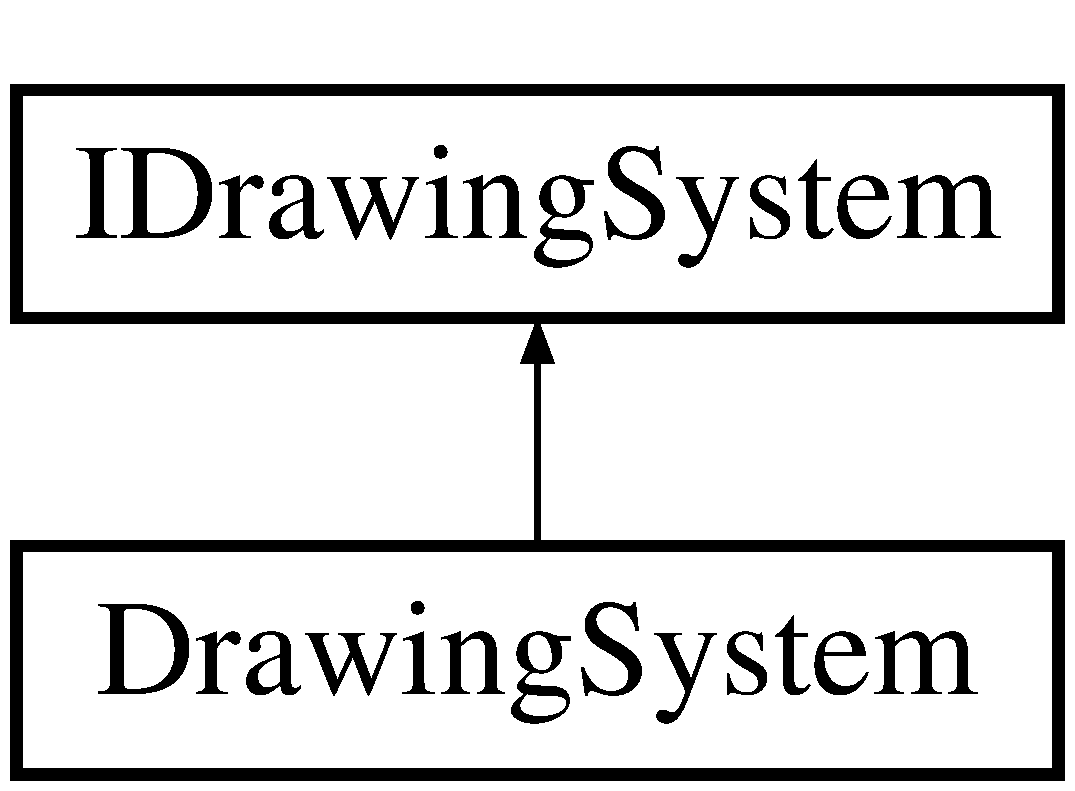
\includegraphics[height=2.000000cm]{classDrawingSystem}
\end{center}
\end{figure}
\subsection*{Public Member Functions}
\begin{DoxyCompactItemize}
\item 
{\bfseries Drawing\+System} (std\+::shared\+\_\+ptr$<$ \hyperlink{classIPrimitivesToDrawContainer}{I\+Primitives\+To\+Draw\+Container} $>$ primitives\+Container)\hypertarget{classDrawingSystem_ac43192217e05834885ac57ff96fcbeb1}{}\label{classDrawingSystem_ac43192217e05834885ac57ff96fcbeb1}

\item 
void {\bfseries draw\+Image} (Image\+Primitive\+Type type, \hyperlink{classPoint}{Point} position, \hyperlink{classRotation}{Rotation} rotation, \hyperlink{classScaleToScreen}{Scale\+To\+Screen} scale, Actor\+Id actor\+Id) override\hypertarget{classDrawingSystem_ae7a1ecfeebb570e4d2d8b6444ca1d5e8}{}\label{classDrawingSystem_ae7a1ecfeebb570e4d2d8b6444ca1d5e8}

\item 
virtual void {\bfseries add\+Removed\+Actor\+Id} (Actor\+Id id) override\hypertarget{classDrawingSystem_a6e4afe9218b8bddfd7c6b0e2cae96c69}{}\label{classDrawingSystem_a6e4afe9218b8bddfd7c6b0e2cae96c69}

\item 
void {\bfseries draw\+Text} (std\+::string text\+Value, \hyperlink{classPoint}{Point} position, Actor\+Id actor\+Id) override\hypertarget{classDrawingSystem_a03b52bea5d3a0f7a826893eb80e09c98}{}\label{classDrawingSystem_a03b52bea5d3a0f7a826893eb80e09c98}

\end{DoxyCompactItemize}


The documentation for this class was generated from the following files\+:\begin{DoxyCompactItemize}
\item 
src/\+Model/\+Model\+Drawing/Drawing\+System.\+h\item 
src/\+Model/\+Model\+Drawing/Drawing\+System.\+cpp\end{DoxyCompactItemize}

\hypertarget{classEmptyScreen}{}\section{Empty\+Screen Class Reference}
\label{classEmptyScreen}\index{Empty\+Screen@{Empty\+Screen}}
Inheritance diagram for Empty\+Screen\+:\begin{figure}[H]
\begin{center}
\leavevmode
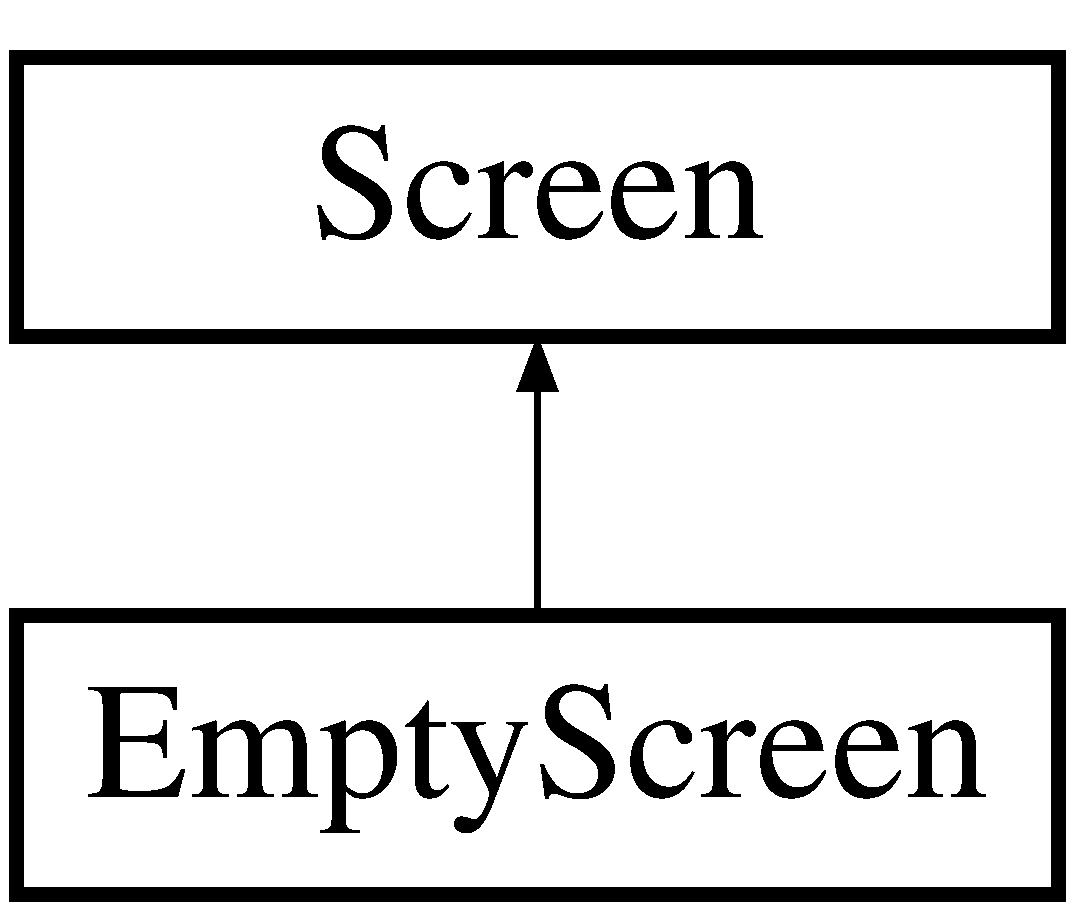
\includegraphics[height=2.000000cm]{classEmptyScreen}
\end{center}
\end{figure}
\subsection*{Public Member Functions}
\begin{DoxyCompactItemize}
\item 
void \hyperlink{classEmptyScreen_acb3da5b502cfb7034c4455ad2ddd7510}{event\+Action} (A\+L\+L\+E\+G\+R\+O\+\_\+\+E\+V\+E\+NT \&, \hyperlink{classViewManager}{View\+Manager} $\ast$, \hyperlink{classGame}{Game} $\ast$)
\item 
void \hyperlink{classEmptyScreen_aa2013df5685b5ef8ae87b3d8605da5b6}{initialize\+Screen\+Elements} ()
\item 
std\+::string \hyperlink{classEmptyScreen_ac392a14c00283e4fff6856a3000b4ecd}{get\+Title} ()
\item 
{\bfseries Empty\+Screen} (std\+::string \&)\hypertarget{classEmptyScreen_acdf0c5dab645394c04a7a28beab25acd}{}\label{classEmptyScreen_acdf0c5dab645394c04a7a28beab25acd}

\end{DoxyCompactItemize}


\subsection{Member Function Documentation}
\index{Empty\+Screen@{Empty\+Screen}!event\+Action@{event\+Action}}
\index{event\+Action@{event\+Action}!Empty\+Screen@{Empty\+Screen}}
\subsubsection[{\texorpdfstring{event\+Action(\+A\+L\+L\+E\+G\+R\+O\+\_\+\+E\+V\+E\+N\+T \&, View\+Manager $\ast$, Game $\ast$)}{eventAction(ALLEGRO_EVENT &, ViewManager *, Game *)}}]{\setlength{\rightskip}{0pt plus 5cm}void Empty\+Screen\+::event\+Action (
\begin{DoxyParamCaption}
\item[{A\+L\+L\+E\+G\+R\+O\+\_\+\+E\+V\+E\+NT \&}]{ev, }
\item[{{\bf View\+Manager} $\ast$}]{vm, }
\item[{{\bf Game} $\ast$}]{g}
\end{DoxyParamCaption}
)\hspace{0.3cm}{\ttfamily [virtual]}}\hypertarget{classEmptyScreen_acb3da5b502cfb7034c4455ad2ddd7510}{}\label{classEmptyScreen_acb3da5b502cfb7034c4455ad2ddd7510}
Virtual method which does some actions when event occurs. 
\begin{DoxyParams}{Parameters}
{\em ev} & event which occured. \\
\hline
{\em vm} & pointer to the \hyperlink{classViewManager}{View\+Manager}. \\
\hline
{\em g} & pointer to the \hyperlink{classGame}{Game}. \\
\hline
\end{DoxyParams}


Reimplemented from \hyperlink{classScreen_a5fb59d03053c2d0aaca26f9480bbe433}{Screen}.

\index{Empty\+Screen@{Empty\+Screen}!get\+Title@{get\+Title}}
\index{get\+Title@{get\+Title}!Empty\+Screen@{Empty\+Screen}}
\subsubsection[{\texorpdfstring{get\+Title()}{getTitle()}}]{\setlength{\rightskip}{0pt plus 5cm}std\+::string Empty\+Screen\+::get\+Title (
\begin{DoxyParamCaption}
{}
\end{DoxyParamCaption}
)\hspace{0.3cm}{\ttfamily [inline]}, {\ttfamily [virtual]}}\hypertarget{classEmptyScreen_ac392a14c00283e4fff6856a3000b4ecd}{}\label{classEmptyScreen_ac392a14c00283e4fff6856a3000b4ecd}
Returns \hyperlink{classScreen}{Screen} title (\hyperlink{classScreen}{Screen} titles are used to organize Screens). \begin{DoxyReturn}{Returns}
title of the screen. 
\end{DoxyReturn}


Reimplemented from \hyperlink{classScreen_a28df2a95a64693e2e5b1238c07c92115}{Screen}.

\index{Empty\+Screen@{Empty\+Screen}!initialize\+Screen\+Elements@{initialize\+Screen\+Elements}}
\index{initialize\+Screen\+Elements@{initialize\+Screen\+Elements}!Empty\+Screen@{Empty\+Screen}}
\subsubsection[{\texorpdfstring{initialize\+Screen\+Elements()}{initializeScreenElements()}}]{\setlength{\rightskip}{0pt plus 5cm}void Empty\+Screen\+::initialize\+Screen\+Elements (
\begin{DoxyParamCaption}
{}
\end{DoxyParamCaption}
)\hspace{0.3cm}{\ttfamily [virtual]}}\hypertarget{classEmptyScreen_aa2013df5685b5ef8ae87b3d8605da5b6}{}\label{classEmptyScreen_aa2013df5685b5ef8ae87b3d8605da5b6}
Virtual method which is used to initialize special elements added to the \hyperlink{classScreen}{Screen} before it will be used 

Reimplemented from \hyperlink{classScreen_a207320477f0e323dc4cd36dbd4706238}{Screen}.



The documentation for this class was generated from the following files\+:\begin{DoxyCompactItemize}
\item 
src/\+View/Empty\+Screen.\+h\item 
src/\+View/Empty\+Screen.\+cpp\end{DoxyCompactItemize}

\hypertarget{classEnumInPythonVisualisator}{}\section{Enum\+In\+Python\+Visualisator Class Reference}
\label{classEnumInPythonVisualisator}\index{Enum\+In\+Python\+Visualisator@{Enum\+In\+Python\+Visualisator}}
Inheritance diagram for Enum\+In\+Python\+Visualisator\+:\begin{figure}[H]
\begin{center}
\leavevmode
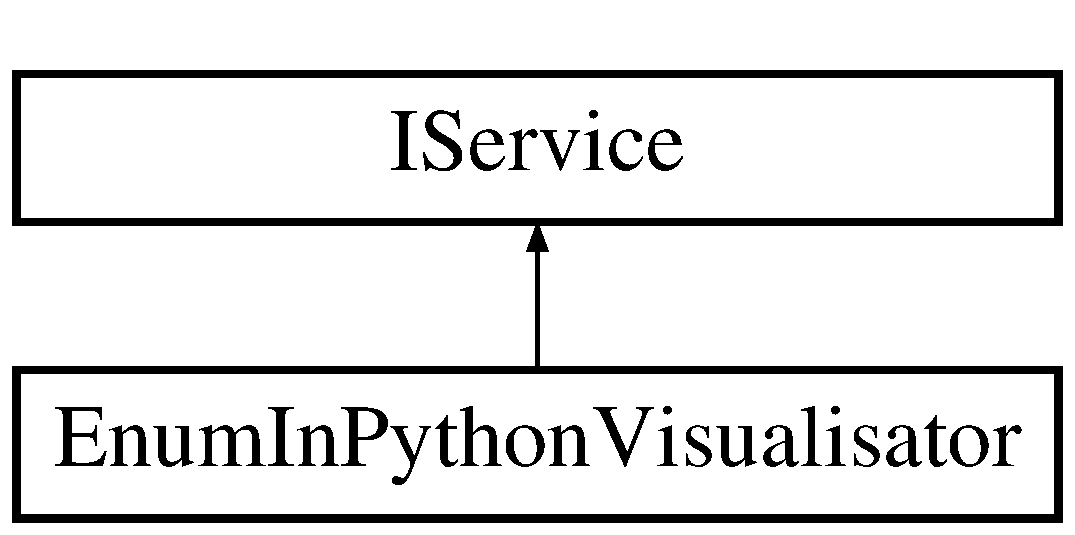
\includegraphics[height=2.000000cm]{classEnumInPythonVisualisator}
\end{center}
\end{figure}
\subsection*{Public Member Functions}
\begin{DoxyCompactItemize}
\item 
{\bfseries Enum\+In\+Python\+Visualisator} (\hyperlink{classPythonModule}{Python\+Module} \&module)\hypertarget{classEnumInPythonVisualisator_a50c757b9491f5824a4a9dc14f27a43a3}{}\label{classEnumInPythonVisualisator_a50c757b9491f5824a4a9dc14f27a43a3}

\item 
virtual void {\bfseries On\+Start} ()\hypertarget{classEnumInPythonVisualisator_afbe8a8d56fbf6bccc821ca1e9ceeb6a5}{}\label{classEnumInPythonVisualisator_afbe8a8d56fbf6bccc821ca1e9ceeb6a5}

\end{DoxyCompactItemize}


The documentation for this class was generated from the following files\+:\begin{DoxyCompactItemize}
\item 
src/\+Model/\+Services/Enum\+In\+Python\+Visualisator.\+h\item 
src/\+Model/\+Services/Enum\+In\+Python\+Visualisator.\+cpp\end{DoxyCompactItemize}

\hypertarget{classExplisionCloudImageManipulatingComponent}{}\section{Explision\+Cloud\+Image\+Manipulating\+Component Class Reference}
\label{classExplisionCloudImageManipulatingComponent}\index{Explision\+Cloud\+Image\+Manipulating\+Component@{Explision\+Cloud\+Image\+Manipulating\+Component}}
Inheritance diagram for Explision\+Cloud\+Image\+Manipulating\+Component\+:\begin{figure}[H]
\begin{center}
\leavevmode
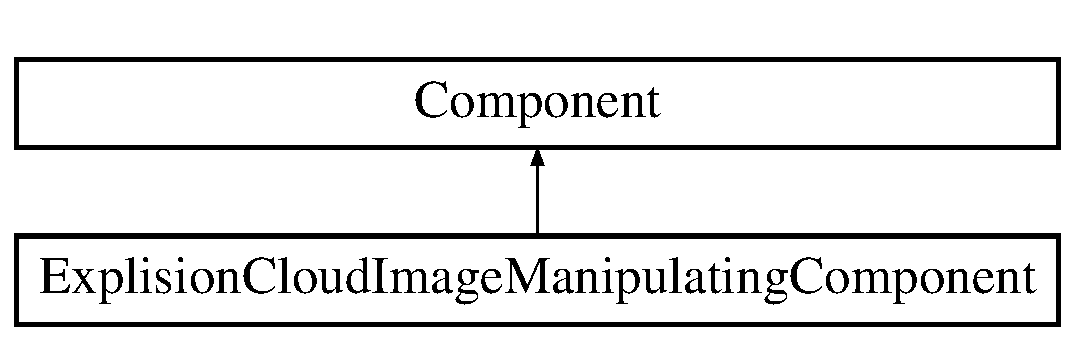
\includegraphics[height=2.000000cm]{classExplisionCloudImageManipulatingComponent}
\end{center}
\end{figure}
\subsection*{Public Member Functions}
\begin{DoxyCompactItemize}
\item 
{\bfseries Explision\+Cloud\+Image\+Manipulating\+Component} (double size\+\_\+, \hyperlink{classGameConfiguration}{Game\+Configuration} \&configuration\+\_\+, std\+::shared\+\_\+ptr$<$ \hyperlink{classActorsContainer}{Actors\+Container} $>$ actors\+Container\+\_\+, const std\+::shared\+\_\+ptr$<$ \hyperlink{classGameTimeProvider}{Game\+Time\+Provider} $>$ \&game\+Time\+Provider\+\_\+)\hypertarget{classExplisionCloudImageManipulatingComponent_ab9733017854e575bec1ecada80ed84f4}{}\label{classExplisionCloudImageManipulatingComponent_ab9733017854e575bec1ecada80ed84f4}

\item 
void {\bfseries On\+Start} (\hyperlink{classIActor}{I\+Actor} \&actor)\hypertarget{classExplisionCloudImageManipulatingComponent_a6e850d437fe31981a9e972c068dd2823}{}\label{classExplisionCloudImageManipulatingComponent_a6e850d437fe31981a9e972c068dd2823}

\item 
void {\bfseries On\+Update} ()\hypertarget{classExplisionCloudImageManipulatingComponent_ab562cbcd8802a2c2f396bdf8c4094321}{}\label{classExplisionCloudImageManipulatingComponent_ab562cbcd8802a2c2f396bdf8c4094321}

\end{DoxyCompactItemize}


The documentation for this class was generated from the following files\+:\begin{DoxyCompactItemize}
\item 
src/\+Model/\+Actors/explosion\+Cloud/Explision\+Cloud\+Image\+Manipulating\+Component.\+h\item 
src/\+Model/\+Actors/explosion\+Cloud/Explision\+Cloud\+Image\+Manipulating\+Component.\+cpp\end{DoxyCompactItemize}

\hypertarget{classExplosionCloudGenerator}{}\section{Explosion\+Cloud\+Generator Class Reference}
\label{classExplosionCloudGenerator}\index{Explosion\+Cloud\+Generator@{Explosion\+Cloud\+Generator}}
\subsection*{Public Member Functions}
\begin{DoxyCompactItemize}
\item 
{\bfseries Explosion\+Cloud\+Generator} (const std\+::shared\+\_\+ptr$<$ \hyperlink{classActorsContainer}{Actors\+Container} $>$ \&actors\+Container, \hyperlink{classActorIdGenerator}{Actor\+Id\+Generator} \&id\+Generator, \hyperlink{classPythonModule}{Python\+Module} \&python\+Module, \hyperlink{classDrawingSystem}{Drawing\+System} \&drawing\+System, \hyperlink{classGameConfiguration}{Game\+Configuration} \&game\+Configuration, \hyperlink{classImageScalesContainer}{Image\+Scales\+Container} \&image\+Scales\+Container, std\+::shared\+\_\+ptr$<$ \hyperlink{classGameTimeProvider}{Game\+Time\+Provider} $>$ game\+Time\+Provider)\hypertarget{classExplosionCloudGenerator_a268fca335920de52fff313734407f396}{}\label{classExplosionCloudGenerator_a268fca335920de52fff313734407f396}

\item 
void {\bfseries generate\+Explosion\+Cloud} (\hyperlink{classPoint}{Point} position, double size)\hypertarget{classExplosionCloudGenerator_aa4e9aa7c9543858cbd97b1a15713b3d3}{}\label{classExplosionCloudGenerator_aa4e9aa7c9543858cbd97b1a15713b3d3}

\end{DoxyCompactItemize}


The documentation for this class was generated from the following files\+:\begin{DoxyCompactItemize}
\item 
src/\+Model/\+Actors/explosion\+Cloud/Explosion\+Cloud\+Generator.\+h\item 
src/\+Model/\+Actors/explosion\+Cloud/Explosion\+Cloud\+Generator.\+cpp\end{DoxyCompactItemize}

\hypertarget{classFakeKeyboardStateToGameProvider}{}\section{Fake\+Keyboard\+State\+To\+Game\+Provider Class Reference}
\label{classFakeKeyboardStateToGameProvider}\index{Fake\+Keyboard\+State\+To\+Game\+Provider@{Fake\+Keyboard\+State\+To\+Game\+Provider}}
\subsection*{Public Member Functions}
\begin{DoxyCompactItemize}
\item 
{\bfseries Fake\+Keyboard\+State\+To\+Game\+Provider} (std\+::shared\+\_\+ptr$<$ \hyperlink{classGame}{Game} $>$ g)\hypertarget{classFakeKeyboardStateToGameProvider_ac597dea55fea1f02a24d79d9f8fd5c33}{}\label{classFakeKeyboardStateToGameProvider_ac597dea55fea1f02a24d79d9f8fd5c33}

\item 
void {\bfseries send\+Keys\+Pressed\+To\+Game} ()\hypertarget{classFakeKeyboardStateToGameProvider_ace89c06296463d0c858c77f6aa4ed1b8}{}\label{classFakeKeyboardStateToGameProvider_ace89c06296463d0c858c77f6aa4ed1b8}

\item 
void {\bfseries add\+Key\+To\+Press} (Keys key)\hypertarget{classFakeKeyboardStateToGameProvider_ada79c8c393bf6c6aba1e3247973c4e62}{}\label{classFakeKeyboardStateToGameProvider_ada79c8c393bf6c6aba1e3247973c4e62}

\end{DoxyCompactItemize}


The documentation for this class was generated from the following files\+:\begin{DoxyCompactItemize}
\item 
test/\+End\+To\+End\+Tests/help/Fake\+Keyboard\+State\+To\+Game\+Provider.\+h\item 
test/\+End\+To\+End\+Tests/help/Fake\+Keyboard\+State\+To\+Game\+Provider.\+cpp\end{DoxyCompactItemize}

\hypertarget{classwhen_1_1ForEveryLoop}{}\section{when\+:\+:For\+Every\+Loop Class Reference}
\label{classwhen_1_1ForEveryLoop}\index{when\+::\+For\+Every\+Loop@{when\+::\+For\+Every\+Loop}}
Inheritance diagram for when\+:\+:For\+Every\+Loop\+:\begin{figure}[H]
\begin{center}
\leavevmode
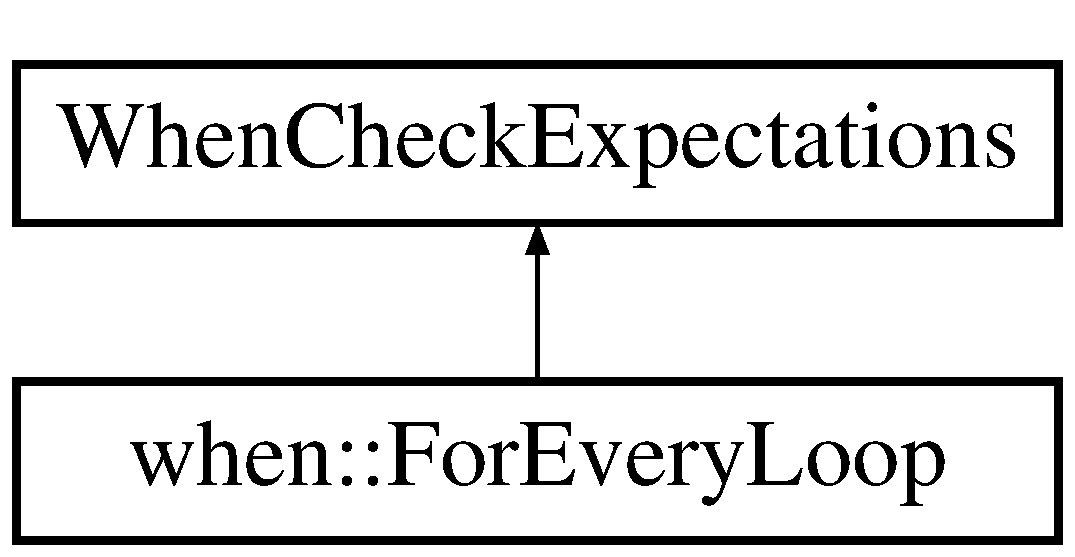
\includegraphics[height=2.000000cm]{classwhen_1_1ForEveryLoop}
\end{center}
\end{figure}
\subsection*{Public Member Functions}
\begin{DoxyCompactItemize}
\item 
virtual bool {\bfseries Check\+Expectations} ()\hypertarget{classwhen_1_1ForEveryLoop_ad982837a130de5d128974f8a8a421205}{}\label{classwhen_1_1ForEveryLoop_ad982837a130de5d128974f8a8a421205}

\end{DoxyCompactItemize}


The documentation for this class was generated from the following files\+:\begin{DoxyCompactItemize}
\item 
test/\+End\+To\+End\+Tests/when/For\+Every\+Loop.\+h\item 
test/\+End\+To\+End\+Tests/when/For\+Every\+Loop.\+cpp\end{DoxyCompactItemize}

\hypertarget{classGame}{}\section{Game Class Reference}
\label{classGame}\index{Game@{Game}}


Main class of model, encapsulates logic of game in separation of graphics liblaries. All servicies used in game are placed as fields.  




{\ttfamily \#include $<$Game.\+h$>$}

\subsection*{Public Member Functions}
\begin{DoxyCompactItemize}
\item 
\hyperlink{classGame_a4983cf735131975a2ff0138fcf7ba4ec}{Game} (\hyperlink{classPoint}{Point} screen\+Resolution, std\+::map$<$ Image\+Primitive\+Type, \hyperlink{classPoint}{Point} $>$ images\+Sizes\+Map)
\begin{DoxyCompactList}\small\item\em Only constructor of \hyperlink{classGame}{Game} class. \end{DoxyCompactList}\item 
void \hyperlink{classGame_a7c48a1b39635e2f1396867845dbf0540}{start\+Single\+Player\+Game} (int difficulty)
\item 
void \hyperlink{classGame_a139e4519b3e9ce6320f56f1ed6738c0b}{start\+Multiplayer\+Game} (int difficulty)
\item 
std\+::shared\+\_\+ptr$<$ \hyperlink{classIOutGameScreenModel}{I\+Out\+Game\+Screen\+Model} $>$ \hyperlink{classGame_adbf1e6c86cc2e767a4ab355fc41484f0}{get\+Out\+Game\+Screen\+Model} ()
\begin{DoxyCompactList}\small\item\em Part of Controller -\/ Model interface. \end{DoxyCompactList}\item 
std\+::shared\+\_\+ptr$<$ \hyperlink{classIInputStateGetter}{I\+Input\+State\+Getter} $>$ \hyperlink{classGame_ab5e270ad252bb80ffcbf0299c3cc28d9}{get\+Input\+State\+Getter} ()
\begin{DoxyCompactList}\small\item\em Part of Controller -\/ Model interface. \end{DoxyCompactList}\item 
\hyperlink{classIInPythonModule}{I\+In\+Python\+Module} \& \hyperlink{classGame_af39898371230b44a33e28bfa8ff6b4da}{get\+In\+Python\+Module} ()
\begin{DoxyCompactList}\small\item\em Part of Controller -\/ Model interface". \end{DoxyCompactList}\item 
\hyperlink{classIOutPythonModule}{I\+Out\+Python\+Module} \& \hyperlink{classGame_a957736283b0b0a9301619b8572dd0f3a}{get\+Out\+Python\+Module} ()
\begin{DoxyCompactList}\small\item\em Part of Controller -\/ Model interface". \end{DoxyCompactList}\item 
std\+::shared\+\_\+ptr$<$ \hyperlink{classIOutGameMusicModel}{I\+Out\+Game\+Music\+Model} $>$ {\bfseries get\+Out\+Game\+Music\+Model} ()\hypertarget{classGame_aae72b8dd502d4ff5668227dbd973273e}{}\label{classGame_aae72b8dd502d4ff5668227dbd973273e}

\item 
void {\bfseries update} ()\hypertarget{classGame_a79df6376b332d63c9eca0dcee30305c3}{}\label{classGame_a79df6376b332d63c9eca0dcee30305c3}

\item 
void {\bfseries set\+Game\+Finished} (int new\+Result)\hypertarget{classGame_a4d87901dd606b9f465ca0ff3ac85b801}{}\label{classGame_a4d87901dd606b9f465ca0ff3ac85b801}

\item 
void {\bfseries set\+Resolution} (\hyperlink{classPoint}{Point} new\+Resolution)\hypertarget{classGame_a507e1c1cab6653f2f7727ac020b46db2}{}\label{classGame_a507e1c1cab6653f2f7727ac020b46db2}

\item 
bool {\bfseries is\+Game\+Finished} ()\hypertarget{classGame_ac210ecbd163be2aa4ad7ae0871656874}{}\label{classGame_ac210ecbd163be2aa4ad7ae0871656874}

\item 
void {\bfseries create\+Both\+Modes\+Actors} ()\hypertarget{classGame_a138adec32f0567e7b027d23e5efee9bc}{}\label{classGame_a138adec32f0567e7b027d23e5efee9bc}

\item 
void {\bfseries create\+Multiplayer\+Actors} ()\hypertarget{classGame_a059bb7a37176b2a121b3309a114fc8bc}{}\label{classGame_a059bb7a37176b2a121b3309a114fc8bc}

\end{DoxyCompactItemize}


\subsection{Detailed Description}
Main class of model, encapsulates logic of game in separation of graphics liblaries. All servicies used in game are placed as fields. 

\subsection{Constructor \& Destructor Documentation}
\index{Game@{Game}!Game@{Game}}
\index{Game@{Game}!Game@{Game}}
\subsubsection[{\texorpdfstring{Game(\+Point screen\+Resolution, std\+::map$<$ Image\+Primitive\+Type, Point $>$ images\+Sizes\+Map)}{Game(Point screenResolution, std::map< ImagePrimitiveType, Point > imagesSizesMap)}}]{\setlength{\rightskip}{0pt plus 5cm}Game\+::\+Game (
\begin{DoxyParamCaption}
\item[{{\bf Point}}]{screen\+Resolution, }
\item[{std\+::map$<$ Image\+Primitive\+Type, {\bf Point} $>$}]{images\+Sizes\+Map}
\end{DoxyParamCaption}
)}\hypertarget{classGame_a4983cf735131975a2ff0138fcf7ba4ec}{}\label{classGame_a4983cf735131975a2ff0138fcf7ba4ec}


Only constructor of \hyperlink{classGame}{Game} class. 


\begin{DoxyParams}{Parameters}
{\em screen\+Resolution} & The resolution which game will start with, this can be changed later. \\
\hline
{\em images\+Sizes\+Map} & Sizes of objects simulated in Box2d are taken from this paramerer/ \\
\hline
\end{DoxyParams}


\subsection{Member Function Documentation}
\index{Game@{Game}!get\+Input\+State\+Getter@{get\+Input\+State\+Getter}}
\index{get\+Input\+State\+Getter@{get\+Input\+State\+Getter}!Game@{Game}}
\subsubsection[{\texorpdfstring{get\+Input\+State\+Getter()}{getInputStateGetter()}}]{\setlength{\rightskip}{0pt plus 5cm}std\+::shared\+\_\+ptr$<$ {\bf I\+Input\+State\+Getter} $>$ Game\+::get\+Input\+State\+Getter (
\begin{DoxyParamCaption}
{}
\end{DoxyParamCaption}
)}\hypertarget{classGame_ab5e270ad252bb80ffcbf0299c3cc28d9}{}\label{classGame_ab5e270ad252bb80ffcbf0299c3cc28d9}


Part of Controller -\/ Model interface. 

\begin{DoxyReturn}{Returns}
object to which input of user is passed to 
\end{DoxyReturn}
\index{Game@{Game}!get\+In\+Python\+Module@{get\+In\+Python\+Module}}
\index{get\+In\+Python\+Module@{get\+In\+Python\+Module}!Game@{Game}}
\subsubsection[{\texorpdfstring{get\+In\+Python\+Module()}{getInPythonModule()}}]{\setlength{\rightskip}{0pt plus 5cm}{\bf I\+In\+Python\+Module} \& Game\+::get\+In\+Python\+Module (
\begin{DoxyParamCaption}
{}
\end{DoxyParamCaption}
)}\hypertarget{classGame_af39898371230b44a33e28bfa8ff6b4da}{}\label{classGame_af39898371230b44a33e28bfa8ff6b4da}


Part of Controller -\/ Model interface". 

\begin{DoxyReturn}{Returns}
object to which python commands are passed 
\end{DoxyReturn}
\index{Game@{Game}!get\+Out\+Game\+Screen\+Model@{get\+Out\+Game\+Screen\+Model}}
\index{get\+Out\+Game\+Screen\+Model@{get\+Out\+Game\+Screen\+Model}!Game@{Game}}
\subsubsection[{\texorpdfstring{get\+Out\+Game\+Screen\+Model()}{getOutGameScreenModel()}}]{\setlength{\rightskip}{0pt plus 5cm}std\+::shared\+\_\+ptr$<$ {\bf I\+Out\+Game\+Screen\+Model} $>$ Game\+::get\+Out\+Game\+Screen\+Model (
\begin{DoxyParamCaption}
{}
\end{DoxyParamCaption}
)}\hypertarget{classGame_adbf1e6c86cc2e767a4ab355fc41484f0}{}\label{classGame_adbf1e6c86cc2e767a4ab355fc41484f0}


Part of Controller -\/ Model interface. 

\begin{DoxyReturn}{Returns}
Shared pointer to field of \hyperlink{classGame}{Game}, which contains data about images and text to be displayed; 
\end{DoxyReturn}
\index{Game@{Game}!get\+Out\+Python\+Module@{get\+Out\+Python\+Module}}
\index{get\+Out\+Python\+Module@{get\+Out\+Python\+Module}!Game@{Game}}
\subsubsection[{\texorpdfstring{get\+Out\+Python\+Module()}{getOutPythonModule()}}]{\setlength{\rightskip}{0pt plus 5cm}{\bf I\+Out\+Python\+Module} \& Game\+::get\+Out\+Python\+Module (
\begin{DoxyParamCaption}
{}
\end{DoxyParamCaption}
)}\hypertarget{classGame_a957736283b0b0a9301619b8572dd0f3a}{}\label{classGame_a957736283b0b0a9301619b8572dd0f3a}


Part of Controller -\/ Model interface". 

\begin{DoxyReturn}{Returns}
objects that contains output of python generated in one loop. 
\end{DoxyReturn}
\index{Game@{Game}!start\+Multiplayer\+Game@{start\+Multiplayer\+Game}}
\index{start\+Multiplayer\+Game@{start\+Multiplayer\+Game}!Game@{Game}}
\subsubsection[{\texorpdfstring{start\+Multiplayer\+Game(int difficulty)}{startMultiplayerGame(int difficulty)}}]{\setlength{\rightskip}{0pt plus 5cm}void Game\+::start\+Multiplayer\+Game (
\begin{DoxyParamCaption}
\item[{int}]{difficulty}
\end{DoxyParamCaption}
)}\hypertarget{classGame_a139e4519b3e9ce6320f56f1ed6738c0b}{}\label{classGame_a139e4519b3e9ce6320f56f1ed6738c0b}

\begin{DoxyParams}{Parameters}
{\em difficulty} & Some settings in Game\+Configuraion are calculated using difficulty setting passed as argument here. \\
\hline
\end{DoxyParams}
\index{Game@{Game}!start\+Single\+Player\+Game@{start\+Single\+Player\+Game}}
\index{start\+Single\+Player\+Game@{start\+Single\+Player\+Game}!Game@{Game}}
\subsubsection[{\texorpdfstring{start\+Single\+Player\+Game(int difficulty)}{startSinglePlayerGame(int difficulty)}}]{\setlength{\rightskip}{0pt plus 5cm}void Game\+::start\+Single\+Player\+Game (
\begin{DoxyParamCaption}
\item[{int}]{difficulty}
\end{DoxyParamCaption}
)}\hypertarget{classGame_a7c48a1b39635e2f1396867845dbf0540}{}\label{classGame_a7c48a1b39635e2f1396867845dbf0540}

\begin{DoxyParams}{Parameters}
{\em difficulty} & Some settings in Game\+Configuraion are calculated using difficulty setting passed as argument here. \\
\hline
\end{DoxyParams}


The documentation for this class was generated from the following files\+:\begin{DoxyCompactItemize}
\item 
src/Game.\+h\item 
src/Game.\+cpp\end{DoxyCompactItemize}

\hypertarget{classGameConfiguration}{}\section{Game\+Configuration Class Reference}
\label{classGameConfiguration}\index{Game\+Configuration@{Game\+Configuration}}
\subsection*{Public Member Functions}
\begin{DoxyCompactItemize}
\item 
{\bfseries Game\+Configuration} (\hyperlink{classPythonModule}{Python\+Module} \&python, \hyperlink{classPoint}{Point} box2d\+Screen\+Dimensions)\hypertarget{classGameConfiguration_a613c9040b73701dc7667820c1b153c3d}{}\label{classGameConfiguration_a613c9040b73701dc7667820c1b153c3d}

\item 
double {\bfseries get\+Max\+Volume} () const \hypertarget{classGameConfiguration_ae37a04f5d833831c1049f279a520220e}{}\label{classGameConfiguration_ae37a04f5d833831c1049f279a520220e}

\item 
void {\bfseries set\+Max\+Volume} (double Max\+Volume)\hypertarget{classGameConfiguration_ab57dae6e0a14e5d259efe074c8e78039}{}\label{classGameConfiguration_ab57dae6e0a14e5d259efe074c8e78039}

\item 
double {\bfseries get\+Volume\+Multiplyer} () const \hypertarget{classGameConfiguration_a6345cbff4a72681c704eb5aa990eb87c}{}\label{classGameConfiguration_a6345cbff4a72681c704eb5aa990eb87c}

\item 
void {\bfseries set\+Volume\+Multiplyer} (double Volume\+Multiplyer)\hypertarget{classGameConfiguration_a791c6583df2565c88be1773092b44e1a}{}\label{classGameConfiguration_a791c6583df2565c88be1773092b44e1a}

\item 
double {\bfseries get\+Explosion\+Cloud\+Fading\+Ratio} () const \hypertarget{classGameConfiguration_acddd17af78a0f245c07c2719aeab580e}{}\label{classGameConfiguration_acddd17af78a0f245c07c2719aeab580e}

\item 
void {\bfseries set\+Explosion\+Cloud\+Fading\+Ratio} (double Explosion\+Cloud\+Fading\+Ratio)\hypertarget{classGameConfiguration_a3438f0da225499cf2ca3583fdcbd0fec}{}\label{classGameConfiguration_a3438f0da225499cf2ca3583fdcbd0fec}

\item 
double {\bfseries get\+Explosion\+Cloud\+Growth\+Ratio} () const \hypertarget{classGameConfiguration_a987f4641ac6a04e60aabcf40022a42fc}{}\label{classGameConfiguration_a987f4641ac6a04e60aabcf40022a42fc}

\item 
void {\bfseries set\+Explosion\+Cloud\+Growth\+Ratio} (double Explosion\+Cloud\+Growth\+Ratio)\hypertarget{classGameConfiguration_a14d98de8fa9361f156856311d9a4be4e}{}\label{classGameConfiguration_a14d98de8fa9361f156856311d9a4be4e}

\item 
\hyperlink{classPoint}{Point} {\bfseries get\+Goodbye\+Message\+Position} () const \hypertarget{classGameConfiguration_a4c39731ab4053f37f205a48d4de45db1}{}\label{classGameConfiguration_a4c39731ab4053f37f205a48d4de45db1}

\item 
void {\bfseries set\+Goodbye\+Message\+Position} (\hyperlink{classPoint}{Point} Goodbye\+Message\+Position)\hypertarget{classGameConfiguration_af1594e686be0257e74c64488f9e03e81}{}\label{classGameConfiguration_af1594e686be0257e74c64488f9e03e81}

\item 
long {\bfseries get\+Min\+Time\+Between\+Powerup\+Generation} () const \hypertarget{classGameConfiguration_a8fcbe588703beb46282310da7865b711}{}\label{classGameConfiguration_a8fcbe588703beb46282310da7865b711}

\item 
void {\bfseries set\+Min\+Time\+Between\+Powerup\+Generation} (long Min\+Time\+Between\+Powerup\+Generation)\hypertarget{classGameConfiguration_af9d45ff31ec41b972cc0e367475db7ab}{}\label{classGameConfiguration_af9d45ff31ec41b972cc0e367475db7ab}

\item 
unsigned int {\bfseries get\+Max\+Powerups\+Count} () const \hypertarget{classGameConfiguration_aa3a5987c7cf509111734d77faefb6f13}{}\label{classGameConfiguration_aa3a5987c7cf509111734d77faefb6f13}

\item 
void {\bfseries set\+Max\+Powerups\+Count} (unsigned int Max\+Powerups\+Count)\hypertarget{classGameConfiguration_a26cd4c01c3adb929a4990d6c4f3a5fa7}{}\label{classGameConfiguration_a26cd4c01c3adb929a4990d6c4f3a5fa7}

\item 
unsigned int {\bfseries get\+Powerup\+Creation\+Propability\+Ratio} () const \hypertarget{classGameConfiguration_ad23f8faab3b63283db26ba99429c0207}{}\label{classGameConfiguration_ad23f8faab3b63283db26ba99429c0207}

\item 
void {\bfseries set\+Powerup\+Creation\+Propability\+Ratio} (unsigned int Powerup\+Creation\+Propability\+Ratio)\hypertarget{classGameConfiguration_a34c382af839fbddb58b398e74e7c27df}{}\label{classGameConfiguration_a34c382af839fbddb58b398e74e7c27df}

\item 
double {\bfseries get\+Min\+Powerup\+Distance\+From\+Rocket} () const \hypertarget{classGameConfiguration_ad1fa18ceed8ed716434aa156b8709761}{}\label{classGameConfiguration_ad1fa18ceed8ed716434aa156b8709761}

\item 
void {\bfseries set\+Min\+Powerup\+Distance\+From\+Rocket} (double Min\+Powerup\+Distance\+From\+Rocket)\hypertarget{classGameConfiguration_a6fb61fbbaea4bbd78e1a4cf2567a461a}{}\label{classGameConfiguration_a6fb61fbbaea4bbd78e1a4cf2567a461a}

\item 
long {\bfseries get\+Temporary\+Rocket\+Shooting\+Component\+Life\+Time} () const \hypertarget{classGameConfiguration_a2e8ed0c3ffb513a5e3d64823cf7edb1f}{}\label{classGameConfiguration_a2e8ed0c3ffb513a5e3d64823cf7edb1f}

\item 
void {\bfseries set\+Temporary\+Rocket\+Shooting\+Component\+Life\+Time} (long Temporary\+Rocket\+Shooting\+Component\+Life\+Time)\hypertarget{classGameConfiguration_ae1640ac78f5c4079e85df7c6de0fc269}{}\label{classGameConfiguration_ae1640ac78f5c4079e85df7c6de0fc269}

\item 
double {\bfseries get\+Rocket\+Opposite\+Acceleration\+Multiply\+Rate} () const \hypertarget{classGameConfiguration_a002bac3f18faca2db44b238e2ca3fc38}{}\label{classGameConfiguration_a002bac3f18faca2db44b238e2ca3fc38}

\item 
void {\bfseries set\+Rocket\+Opposite\+Acceleration\+Multiply\+Rate} (double Rocket\+Opposite\+Acceleration\+Multiply\+Rate)\hypertarget{classGameConfiguration_aef5ea973357aba6f6e7909c15b5cc489}{}\label{classGameConfiguration_aef5ea973357aba6f6e7909c15b5cc489}

\item 
\hyperlink{classPoint}{Point} {\bfseries get\+Screen\+Size\+In\+Pixels} () const \hypertarget{classGameConfiguration_a3fd31a20d1dc67bad75a97a565ae24db}{}\label{classGameConfiguration_a3fd31a20d1dc67bad75a97a565ae24db}

\item 
void {\bfseries set\+Screen\+Size\+In\+Pixels} (\hyperlink{classPoint}{Point} new\+Size)\hypertarget{classGameConfiguration_aab19b78782deebf894c620221e191d7e}{}\label{classGameConfiguration_aab19b78782deebf894c620221e191d7e}

\item 
\hyperlink{classPoint}{Point} {\bfseries get\+Initial\+Position} () const \hypertarget{classGameConfiguration_ace6795655ac1a88974356c99810f7e4d}{}\label{classGameConfiguration_ace6795655ac1a88974356c99810f7e4d}

\item 
void {\bfseries set\+Initial\+Position} (\hyperlink{classPoint}{Point} Initial\+Position)\hypertarget{classGameConfiguration_abac5bb94f2284ceb822d08e24c576b0a}{}\label{classGameConfiguration_abac5bb94f2284ceb822d08e24c576b0a}

\item 
\hyperlink{classRotation}{Rotation} {\bfseries get\+Initial\+Rotation} () const \hypertarget{classGameConfiguration_ac57cba6d998f6a3e73d64c445dc322af}{}\label{classGameConfiguration_ac57cba6d998f6a3e73d64c445dc322af}

\item 
void {\bfseries set\+Initial\+Rotation} (\hyperlink{classRotation}{Rotation} Initial\+Rotation)\hypertarget{classGameConfiguration_a84249397382d4d36fc3dd3a03839c10e}{}\label{classGameConfiguration_a84249397382d4d36fc3dd3a03839c10e}

\item 
double {\bfseries get\+Rocket\+Acceleration\+Rate} () const \hypertarget{classGameConfiguration_ae6b5a001a2b8716df1c013193170fe03}{}\label{classGameConfiguration_ae6b5a001a2b8716df1c013193170fe03}

\item 
void {\bfseries set\+Rocket\+Acceleration\+Rate} (double Rocket\+Acceleration\+Rate)\hypertarget{classGameConfiguration_af7dae5f1431544fd6bf5d53bf9434170}{}\label{classGameConfiguration_af7dae5f1431544fd6bf5d53bf9434170}

\item 
double {\bfseries get\+Rocket\+Turn\+Rate} () const \hypertarget{classGameConfiguration_acb6e6e9a9b12c86db6f52d0c06c96622}{}\label{classGameConfiguration_acb6e6e9a9b12c86db6f52d0c06c96622}

\item 
void {\bfseries set\+Rocket\+Turn\+Rate} (double Rocket\+Turn\+Rate)\hypertarget{classGameConfiguration_adc79b8b9c90fc412aebb6e497454623b}{}\label{classGameConfiguration_adc79b8b9c90fc412aebb6e497454623b}

\item 
\hyperlink{classScaleToScreen}{Scale\+To\+Screen} {\bfseries get\+Rocket\+Scale\+To\+Screen} () const \hypertarget{classGameConfiguration_aee4b4d84ef6eddba7578217c94cb5f0c}{}\label{classGameConfiguration_aee4b4d84ef6eddba7578217c94cb5f0c}

\item 
void {\bfseries set\+Rocket\+Scale\+To\+Screen} (\hyperlink{classScaleToScreen}{Scale\+To\+Screen} Rocket\+Scale\+To\+Screen)\hypertarget{classGameConfiguration_a6511ac6ed0dcf74f0bca75addc74345a}{}\label{classGameConfiguration_a6511ac6ed0dcf74f0bca75addc74345a}

\item 
float {\bfseries get\+Distance\+Between\+Rocket\+And\+Tail} () const \hypertarget{classGameConfiguration_af72c0d2e65c7b97cf845a9b552f06fda}{}\label{classGameConfiguration_af72c0d2e65c7b97cf845a9b552f06fda}

\item 
void {\bfseries set\+Distance\+Between\+Rocket\+And\+Tail} (float Distance\+Between\+Rocket\+And\+Tail)\hypertarget{classGameConfiguration_a6ef296f93ebfc95a2d2714090dad637c}{}\label{classGameConfiguration_a6ef296f93ebfc95a2d2714090dad637c}

\item 
\hyperlink{classScaleToScreen}{Scale\+To\+Screen} {\bfseries get\+Box2d\+To\+Allegro\+Scale} () const \hypertarget{classGameConfiguration_abacc05464dd8bca8158ea98b827cf33d}{}\label{classGameConfiguration_abacc05464dd8bca8158ea98b827cf33d}

\item 
void {\bfseries set\+Box2d\+To\+Allegro\+Scale} (\hyperlink{classScaleToScreen}{Scale\+To\+Screen} Box2d\+To\+Allegro\+Scale)\hypertarget{classGameConfiguration_a6a035965067079a19243884b15d69da6}{}\label{classGameConfiguration_a6a035965067079a19243884b15d69da6}

\item 
\hyperlink{classScaleToScreen}{Scale\+To\+Screen} {\bfseries get\+Allegro\+To\+Box2d\+Scale} () const \hypertarget{classGameConfiguration_a02bd71b4bdbdf12375d8166ff51e8ffa}{}\label{classGameConfiguration_a02bd71b4bdbdf12375d8166ff51e8ffa}

\item 
void {\bfseries set\+Allegro\+To\+Box2d\+Scale} (\hyperlink{classScaleToScreen}{Scale\+To\+Screen} Allegro\+To\+Box2d\+Scale)\hypertarget{classGameConfiguration_a477eb4c18409b56643d36c08114a828c}{}\label{classGameConfiguration_a477eb4c18409b56643d36c08114a828c}

\item 
\hyperlink{classPoint}{Point} {\bfseries get\+Box2d\+Screen\+Dimensions} () const \hypertarget{classGameConfiguration_af0e7f4289f2e99cae96ca3b301af560b}{}\label{classGameConfiguration_af0e7f4289f2e99cae96ca3b301af560b}

\item 
void {\bfseries set\+Box2d\+Screen\+Dimensions} (\hyperlink{classPoint}{Point} Box2d\+Screen\+DimensionsX)\hypertarget{classGameConfiguration_ac7eca49d46dcc1ed7fd972bb07699a13}{}\label{classGameConfiguration_ac7eca49d46dcc1ed7fd972bb07699a13}

\item 
\hyperlink{classPoint}{Point} {\bfseries get\+Duplication\+Boundaries\+Size} () const \hypertarget{classGameConfiguration_a17f259cb926de5ded2b28f77c880dcaf}{}\label{classGameConfiguration_a17f259cb926de5ded2b28f77c880dcaf}

\item 
void {\bfseries set\+Duplication\+Boundaries\+Size} (\hyperlink{classPoint}{Point} Duplication\+Boundaries\+Size)\hypertarget{classGameConfiguration_aa41df33fff977a2950b3c001e2641684}{}\label{classGameConfiguration_aa41df33fff977a2950b3c001e2641684}

\item 
Actor\+Id {\bfseries get\+Boundaries\+Duplicate\+Actor\+Id\+Offset} () const \hypertarget{classGameConfiguration_a4360542ed9767f34262e434babc41d39}{}\label{classGameConfiguration_a4360542ed9767f34262e434babc41d39}

\item 
void {\bfseries set\+Boundaries\+Duplicate\+Actor\+Id\+Offset} (Actor\+Id Boundaries\+Duplicate\+Actor\+Id\+Offset)\hypertarget{classGameConfiguration_a781ddd1d05b3fff5e804a58095c4f51e}{}\label{classGameConfiguration_a781ddd1d05b3fff5e804a58095c4f51e}

\item 
unsigned int {\bfseries get\+Asteroid\+Creation\+Propability\+Ratio} () const \hypertarget{classGameConfiguration_a3e80e3466cc4766edd17badb0aec3cad}{}\label{classGameConfiguration_a3e80e3466cc4766edd17badb0aec3cad}

\item 
void {\bfseries set\+Asteroid\+Creation\+Propability\+Ratio} (unsigned int Asteroid\+Creation\+Propability\+Ratio)\hypertarget{classGameConfiguration_a07bc752c7071100bbf12b22a98018a0a}{}\label{classGameConfiguration_a07bc752c7071100bbf12b22a98018a0a}

\item 
unsigned int {\bfseries get\+Min\+Time\+Between\+Asteroids\+Creation} () const \hypertarget{classGameConfiguration_ab14c64e9479f5ff27dfbbbe74922b93d}{}\label{classGameConfiguration_ab14c64e9479f5ff27dfbbbe74922b93d}

\item 
void {\bfseries set\+Min\+Time\+Between\+Asteroids\+Creation} (unsigned int Min\+Time\+Between\+Asteroids\+Creation)\hypertarget{classGameConfiguration_a0ebad81e5deab674787b1c3367bd7862}{}\label{classGameConfiguration_a0ebad81e5deab674787b1c3367bd7862}

\item 
unsigned int {\bfseries get\+Max\+Asteroids\+Count} () const \hypertarget{classGameConfiguration_a9e2d8d296a8d7e59847a716872bd7d6b}{}\label{classGameConfiguration_a9e2d8d296a8d7e59847a716872bd7d6b}

\item 
void {\bfseries set\+Max\+Asteroids\+Count} (unsigned int Max\+Asteroids\+Count)\hypertarget{classGameConfiguration_a2c6e0d4a84aa3b4cb2a2b9e5f1278610}{}\label{classGameConfiguration_a2c6e0d4a84aa3b4cb2a2b9e5f1278610}

\item 
\hyperlink{classPoint}{Point} {\bfseries get\+Asteroids\+Generation\+Boundaries\+Size} () const \hypertarget{classGameConfiguration_ae7c38ee9b8c1fb36cd3a1f7ce5973b62}{}\label{classGameConfiguration_ae7c38ee9b8c1fb36cd3a1f7ce5973b62}

\item 
void {\bfseries set\+Asteroids\+Generation\+Boundaries\+Size} (\hyperlink{classPoint}{Point} Asteroids\+Generation\+Boundaries\+Size)\hypertarget{classGameConfiguration_ae1393d9cf456cb47ddd283886e743648}{}\label{classGameConfiguration_ae1393d9cf456cb47ddd283886e743648}

\item 
double {\bfseries get\+Asteroid\+Max\+Initial\+Impulse} () const \hypertarget{classGameConfiguration_acaff39b0af75f67dbc95a782d67c9169}{}\label{classGameConfiguration_acaff39b0af75f67dbc95a782d67c9169}

\item 
void {\bfseries set\+Asteroid\+Max\+Initial\+Impulse} (double Asteroid\+Max\+Initial\+Impulse)\hypertarget{classGameConfiguration_af4e2f882c3b4bc0fcc28ea560fb17636}{}\label{classGameConfiguration_af4e2f882c3b4bc0fcc28ea560fb17636}

\item 
double {\bfseries get\+Asteroid\+Min\+Initial\+Impulse} () const \hypertarget{classGameConfiguration_ae464b394e5cf22cc9588a3a9071e6563}{}\label{classGameConfiguration_ae464b394e5cf22cc9588a3a9071e6563}

\item 
void {\bfseries set\+Asteroid\+Min\+Initial\+Impulse} (double Asteroid\+Min\+Initial\+Impulse)\hypertarget{classGameConfiguration_aa9030efe9e84388acb960313a2c6baca}{}\label{classGameConfiguration_aa9030efe9e84388acb960313a2c6baca}

\item 
double {\bfseries get\+Asteroid\+Min\+Size} () const \hypertarget{classGameConfiguration_a656ed95533f80d9dd529790487281ca4}{}\label{classGameConfiguration_a656ed95533f80d9dd529790487281ca4}

\item 
void {\bfseries set\+Asteroid\+Min\+Size} (double Asteroid\+Min\+Size)\hypertarget{classGameConfiguration_ae9571295579a14d194aa323fd18d1af5}{}\label{classGameConfiguration_ae9571295579a14d194aa323fd18d1af5}

\item 
double {\bfseries get\+Asteroid\+Max\+Size} () const \hypertarget{classGameConfiguration_a6682cb792406d5a608305c456a0cbc70}{}\label{classGameConfiguration_a6682cb792406d5a608305c456a0cbc70}

\item 
void {\bfseries set\+Asteroid\+Max\+Size} (double Asteroid\+Max\+Size)\hypertarget{classGameConfiguration_a5cfae7eea03c34f7cc097e3c667b6335}{}\label{classGameConfiguration_a5cfae7eea03c34f7cc097e3c667b6335}

\item 
double {\bfseries get\+Asteroid\+Max\+Rotation\+Speed} () const \hypertarget{classGameConfiguration_a35c00d7f7818d59d76b9a63589c9bfa3}{}\label{classGameConfiguration_a35c00d7f7818d59d76b9a63589c9bfa3}

\item 
void {\bfseries set\+Asteroid\+Max\+Rotation\+Speed} (double Asteroid\+Max\+Rotation\+Speed)\hypertarget{classGameConfiguration_a87f4ca20e42bd2d07f292a8e2596a1d2}{}\label{classGameConfiguration_a87f4ca20e42bd2d07f292a8e2596a1d2}

\item 
\hyperlink{classRect}{Rect} {\bfseries get\+Actors\+Destroy\+Rectangle} () const \hypertarget{classGameConfiguration_a6c4f151aedb397cd7b7fa8ede6aa9c01}{}\label{classGameConfiguration_a6c4f151aedb397cd7b7fa8ede6aa9c01}

\item 
void {\bfseries set\+Actors\+Destroy\+Rectangle} (\hyperlink{classRect}{Rect} Actors\+Destroy\+Rectangle)\hypertarget{classGameConfiguration_ad2b1d277b902ff84873f5f29092bc969}{}\label{classGameConfiguration_ad2b1d277b902ff84873f5f29092bc969}

\item 
unsigned long {\bfseries get\+Min\+Time\+Between\+Shots} () const \hypertarget{classGameConfiguration_a5ab85a55d0dc5bc1ebe84a2cbe6ec4ab}{}\label{classGameConfiguration_a5ab85a55d0dc5bc1ebe84a2cbe6ec4ab}

\item 
void {\bfseries set\+Min\+Time\+Between\+Shots} (unsigned long Min\+Time\+Between\+Shots)\hypertarget{classGameConfiguration_adb04c39017aa07d76e61d7bcf9d29572}{}\label{classGameConfiguration_adb04c39017aa07d76e61d7bcf9d29572}

\item 
double {\bfseries get\+Distance\+Between\+Rocket\+And\+Projectile} () const \hypertarget{classGameConfiguration_adac56f6b7bd6c6867b659f5b249cd32f}{}\label{classGameConfiguration_adac56f6b7bd6c6867b659f5b249cd32f}

\item 
void {\bfseries set\+Distance\+Between\+Rocket\+And\+Projectile} (double Distance\+Between\+Rocket\+And\+Projectile)\hypertarget{classGameConfiguration_a0e20e5002bf99765f93ed8b5246e1ba3}{}\label{classGameConfiguration_a0e20e5002bf99765f93ed8b5246e1ba3}

\item 
double {\bfseries get\+Projectile\+Speed} () const \hypertarget{classGameConfiguration_ad993486abf46a54ae53dd7511a8ed485}{}\label{classGameConfiguration_ad993486abf46a54ae53dd7511a8ed485}

\item 
void {\bfseries set\+Projectile\+Speed} (double Projectile\+Speed)\hypertarget{classGameConfiguration_a97eecc15961cd583ed6c65cfa482529c}{}\label{classGameConfiguration_a97eecc15961cd583ed6c65cfa482529c}

\item 
unsigned int {\bfseries get\+Initial\+Rocket\+Life} () const \hypertarget{classGameConfiguration_a0715156a35713b5e9ac0e86571e2581b}{}\label{classGameConfiguration_a0715156a35713b5e9ac0e86571e2581b}

\item 
void {\bfseries set\+Initial\+Rocket\+Life} (unsigned int Initial\+Rocket\+Life)\hypertarget{classGameConfiguration_a07661f40535440be2e16e1789f2cbf0b}{}\label{classGameConfiguration_a07661f40535440be2e16e1789f2cbf0b}

\item 
unsigned int {\bfseries get\+Times\+Rocket\+Image\+Is\+Flickering} () const \hypertarget{classGameConfiguration_a035411318454ed12fb5c370377a20544}{}\label{classGameConfiguration_a035411318454ed12fb5c370377a20544}

\item 
void {\bfseries set\+Times\+Rocket\+Image\+Is\+Flickering} (unsigned int Times\+Rocket\+Image\+Is\+Flickering)\hypertarget{classGameConfiguration_a66004b697ef7a6e55e33fc93742ef9ac}{}\label{classGameConfiguration_a66004b697ef7a6e55e33fc93742ef9ac}

\item 
unsigned long {\bfseries get\+Timeof\+One\+Flicker} () const \hypertarget{classGameConfiguration_a4193af7729d1cbfa355f075e0b73c528}{}\label{classGameConfiguration_a4193af7729d1cbfa355f075e0b73c528}

\item 
void {\bfseries set\+Timeof\+One\+Flicker} (unsigned long Timeof\+One\+Flicker)\hypertarget{classGameConfiguration_a926e569d7576312e8b43de718f69b7aa}{}\label{classGameConfiguration_a926e569d7576312e8b43de718f69b7aa}

\item 
\hyperlink{classPoint}{Point} {\bfseries get\+Initial\+Heart\+Position} () const \hypertarget{classGameConfiguration_a1817c7f99ec4684a851175a7b9144089}{}\label{classGameConfiguration_a1817c7f99ec4684a851175a7b9144089}

\item 
void {\bfseries set\+Initial\+Heart\+Position} (\hyperlink{classPoint}{Point} Initial\+Heart\+Position)\hypertarget{classGameConfiguration_a5cb6f0eaba156234cd3bcf2d5bae9b2f}{}\label{classGameConfiguration_a5cb6f0eaba156234cd3bcf2d5bae9b2f}

\item 
unsigned int {\bfseries get\+Max\+Rocket\+Lifes} () const \hypertarget{classGameConfiguration_ac33d3c3d156490f1bafb710dcccecbef}{}\label{classGameConfiguration_ac33d3c3d156490f1bafb710dcccecbef}

\item 
void {\bfseries set\+Max\+Rocket\+Lifes} (unsigned int Max\+Rocket\+Lifes)\hypertarget{classGameConfiguration_a99e6730418254cdb11c4007e3749de05}{}\label{classGameConfiguration_a99e6730418254cdb11c4007e3749de05}

\item 
\hyperlink{classPoint}{Point} {\bfseries get\+Score\+Text\+Position} () const \hypertarget{classGameConfiguration_a7ad4eb7d0e789b295c244ce65939a9c7}{}\label{classGameConfiguration_a7ad4eb7d0e789b295c244ce65939a9c7}

\item 
void {\bfseries set\+Score\+Text\+Position} (\hyperlink{classPoint}{Point} Score\+Text\+Position)\hypertarget{classGameConfiguration_a6adc82174256c8c537bfde342148aeab}{}\label{classGameConfiguration_a6adc82174256c8c537bfde342148aeab}

\item 
unsigned int {\bfseries get\+Score\+By\+Destroying\+Asteroid} () const \hypertarget{classGameConfiguration_a02b275ca12b11c1a8608a0b14dccb0f6}{}\label{classGameConfiguration_a02b275ca12b11c1a8608a0b14dccb0f6}

\item 
void {\bfseries set\+Score\+By\+Destroying\+Asteroid} (unsigned int Score\+By\+Destroying\+Asteroid)\hypertarget{classGameConfiguration_a69e1aab9cce1cac74bc30a73f6264ba8}{}\label{classGameConfiguration_a69e1aab9cce1cac74bc30a73f6264ba8}

\item 
unsigned long {\bfseries get\+Min\+Time\+Between\+Second\+Player\+Shoots} () const \hypertarget{classGameConfiguration_a9e879a96422309a56dd55aacc59340e7}{}\label{classGameConfiguration_a9e879a96422309a56dd55aacc59340e7}

\item 
void {\bfseries set\+Min\+Time\+Between\+Second\+Player\+Shoots} (unsigned long Min\+Time\+Between\+Second\+Player\+Shoots)\hypertarget{classGameConfiguration_a16fd8d0740fcb8b402f302514e2f257e}{}\label{classGameConfiguration_a16fd8d0740fcb8b402f302514e2f257e}

\item 
double {\bfseries get\+Second\+Player\+Asteroid\+Velocity\+Multiplayer} () const \hypertarget{classGameConfiguration_a524ac4cd586a42bdbe49b75d93efa0cf}{}\label{classGameConfiguration_a524ac4cd586a42bdbe49b75d93efa0cf}

\item 
void {\bfseries set\+Second\+Player\+Asteroid\+Velocity\+Multiplayer} (double Second\+Player\+Asteroid\+Velocity\+Multiplayer)\hypertarget{classGameConfiguration_ad0ccfa32f5d4885b01635207005f945d}{}\label{classGameConfiguration_ad0ccfa32f5d4885b01635207005f945d}

\item 
double {\bfseries get\+Second\+Player\+Asteroid\+Size\+Divider} () const \hypertarget{classGameConfiguration_adbaf033a5a169fa357a75582cba19f6a}{}\label{classGameConfiguration_adbaf033a5a169fa357a75582cba19f6a}

\item 
void {\bfseries set\+Second\+Player\+Asteroid\+Size\+Divider} (double Second\+Player\+Asteroid\+Size\+Divider)\hypertarget{classGameConfiguration_ae30b6a490141f7df327f9ce6622e6bd3}{}\label{classGameConfiguration_ae30b6a490141f7df327f9ce6622e6bd3}

\item 
double {\bfseries get\+Min\+Second\+Player\+Asteroid\+Size} () const \hypertarget{classGameConfiguration_a93317a57ca18286a7ec523969d6da306}{}\label{classGameConfiguration_a93317a57ca18286a7ec523969d6da306}

\item 
void {\bfseries set\+Min\+Second\+Player\+Asteroid\+Size} (double Min\+Second\+Player\+Asteroid\+Size)\hypertarget{classGameConfiguration_a0075edec70545f10661e4f0df489fd36}{}\label{classGameConfiguration_a0075edec70545f10661e4f0df489fd36}

\item 
double {\bfseries get\+Max\+Second\+Player\+Asteroid\+Size} () const \hypertarget{classGameConfiguration_a039d07fa3d4253f3a8125338a904af63}{}\label{classGameConfiguration_a039d07fa3d4253f3a8125338a904af63}

\item 
void {\bfseries set\+Max\+Second\+Player\+Asteroid\+Size} (double Max\+Second\+Player\+Asteroid\+Size)\hypertarget{classGameConfiguration_ad6092534e7711dc2701d6e203aaba9b4}{}\label{classGameConfiguration_ad6092534e7711dc2701d6e203aaba9b4}

\item 
std\+::string {\bfseries get\+On\+Update\+Python\+Script\+Path} () const \hypertarget{classGameConfiguration_a27ba0a4a27c18b520672997b6d2a020f}{}\label{classGameConfiguration_a27ba0a4a27c18b520672997b6d2a020f}

\item 
void {\bfseries set\+On\+Update\+Python\+Script\+Path} (std\+::string On\+Update\+Python\+Script\+Path)\hypertarget{classGameConfiguration_a5e8d6f1b06ba4a4b95cd8f9ee75a00d9}{}\label{classGameConfiguration_a5e8d6f1b06ba4a4b95cd8f9ee75a00d9}

\item 
std\+::string {\bfseries get\+On\+Start\+Python\+Script\+Path} () const \hypertarget{classGameConfiguration_acd1eb75a6533b021b8b4b40e1ca91b6a}{}\label{classGameConfiguration_acd1eb75a6533b021b8b4b40e1ca91b6a}

\item 
void {\bfseries set\+On\+Start\+Python\+Script\+Path} (std\+::string On\+Start\+Python\+Script\+Path)\hypertarget{classGameConfiguration_a998f31704d2ec92f91a9e8b465e15410}{}\label{classGameConfiguration_a998f31704d2ec92f91a9e8b465e15410}

\end{DoxyCompactItemize}
\subsection*{Static Public Attributes}
\begin{DoxyCompactItemize}
\item 
static \hyperlink{classGameConfiguration}{Game\+Configuration} $\ast$ {\bfseries only\+Instance\+Pointer}\hypertarget{classGameConfiguration_a4abb60f0f416e1c5f5bcbf5a94b48789}{}\label{classGameConfiguration_a4abb60f0f416e1c5f5bcbf5a94b48789}

\end{DoxyCompactItemize}


The documentation for this class was generated from the following files\+:\begin{DoxyCompactItemize}
\item 
src/\+Model/configuration/Game\+Configuration.\+h\item 
src/\+Model/configuration/Game\+Configuration.\+cpp\end{DoxyCompactItemize}

\hypertarget{classGameEndingIndicatingService}{}\section{Game\+Ending\+Indicating\+Service Class Reference}
\label{classGameEndingIndicatingService}\index{Game\+Ending\+Indicating\+Service@{Game\+Ending\+Indicating\+Service}}
Inheritance diagram for Game\+Ending\+Indicating\+Service\+:\begin{figure}[H]
\begin{center}
\leavevmode
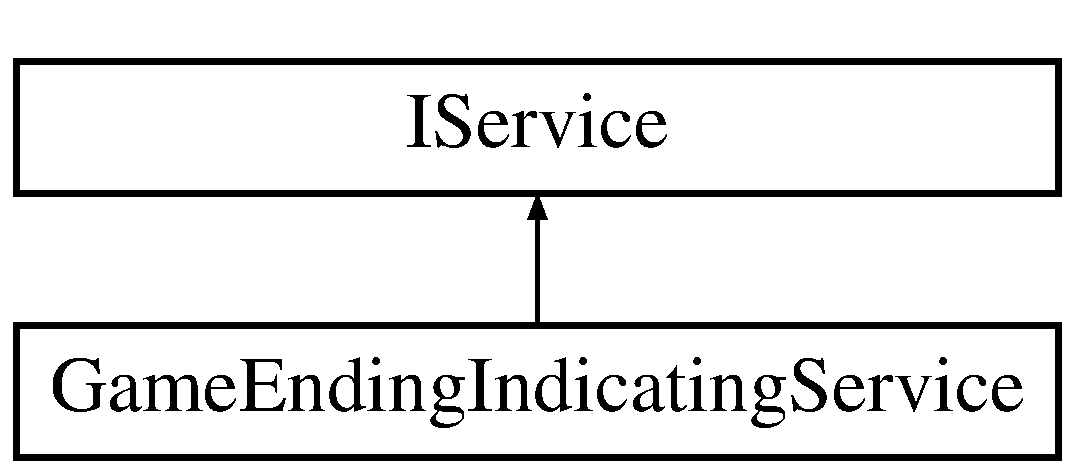
\includegraphics[height=2.000000cm]{classGameEndingIndicatingService}
\end{center}
\end{figure}
\subsection*{Public Member Functions}
\begin{DoxyCompactItemize}
\item 
{\bfseries Game\+Ending\+Indicating\+Service} (\hyperlink{classRocketLife}{Rocket\+Life} \&rocket\+Life\+\_\+, \hyperlink{classScoreCount}{Score\+Count} \&score\+Count\+\_\+, std\+::shared\+\_\+ptr$<$ \hyperlink{classGameStopService}{Game\+Stop\+Service} $>$ game\+Stop\+Service\+\_\+, \hyperlink{classGame}{Game} \&game\+\_\+, Actor\+Id score\+Id, \hyperlink{classGameConfiguration}{Game\+Configuration} \&configuration, \hyperlink{classIDrawingSystem}{I\+Drawing\+System} \&drawing\+System, std\+::shared\+\_\+ptr$<$ \hyperlink{classIInputStateProvider}{I\+Input\+State\+Provider} $>$ input\+State\+Provider)\hypertarget{classGameEndingIndicatingService_af6b266236264bbbfe21db486f9c64fb3}{}\label{classGameEndingIndicatingService_af6b266236264bbbfe21db486f9c64fb3}

\item 
void {\bfseries On\+Update} ()\hypertarget{classGameEndingIndicatingService_aed09cbea0f7e1280a7bbdbca1aee6882}{}\label{classGameEndingIndicatingService_aed09cbea0f7e1280a7bbdbca1aee6882}

\item 
void {\bfseries reset} ()\hypertarget{classGameEndingIndicatingService_a700c3c05db4f7e4d164173136012b00d}{}\label{classGameEndingIndicatingService_a700c3c05db4f7e4d164173136012b00d}

\end{DoxyCompactItemize}


The documentation for this class was generated from the following files\+:\begin{DoxyCompactItemize}
\item 
src/\+Model/\+Services/Game\+Ending\+Indicating\+Service.\+h\item 
src/\+Model/\+Services/Game\+Ending\+Indicating\+Service.\+cpp\end{DoxyCompactItemize}

\hypertarget{classGameRunner}{}\section{Game\+Runner Class Reference}
\label{classGameRunner}\index{Game\+Runner@{Game\+Runner}}
\subsection*{Public Member Functions}
\begin{DoxyCompactItemize}
\item 
void {\bfseries Add\+Each\+Loop\+Expectations} (std\+::shared\+\_\+ptr$<$ \hyperlink{classIEndToEndExpectation}{I\+End\+To\+End\+Expectation} $>$ new\+Expectation)\hypertarget{classGameRunner_a02e5260aca1b02222229e5de7b7bab35}{}\label{classGameRunner_a02e5260aca1b02222229e5de7b7bab35}

\item 
void {\bfseries Add\+First\+Loop\+Expectations} (std\+::shared\+\_\+ptr$<$ \hyperlink{classIEndToEndExpectation}{I\+End\+To\+End\+Expectation} $>$ new\+Expectation)\hypertarget{classGameRunner_a967f98898ffcac8d4aca6230607446ea}{}\label{classGameRunner_a967f98898ffcac8d4aca6230607446ea}

\item 
void {\bfseries Add\+After\+Run\+Expectations} (std\+::shared\+\_\+ptr$<$ \hyperlink{classIEndToEndExpectation}{I\+End\+To\+End\+Expectation} $>$ new\+Expectation)\hypertarget{classGameRunner_a74b8c7f031062743104a31f6d453b637}{}\label{classGameRunner_a74b8c7f031062743104a31f6d453b637}

\item 
std\+::string {\bfseries create\+Error\+Message} (std\+::shared\+\_\+ptr$<$ \hyperlink{classIEndToEndExpectation}{I\+End\+To\+End\+Expectation} $>$ failed\+Expectation)\hypertarget{classGameRunner_a8e6ab5e54a322f9b13123758d457f1e7}{}\label{classGameRunner_a8e6ab5e54a322f9b13123758d457f1e7}

\item 
void {\bfseries Run\+For\+Loops} (int loops\+To\+Run)\hypertarget{classGameRunner_aa0c9e410e8df3b074860ea3a7fe4f8d1}{}\label{classGameRunner_aa0c9e410e8df3b074860ea3a7fe4f8d1}

\item 
void {\bfseries Add\+Key\+Pressed} (Keys key\+Pressed)\hypertarget{classGameRunner_aba2c9bd5cb90c4567b664733ca3f965d}{}\label{classGameRunner_aba2c9bd5cb90c4567b664733ca3f965d}

\item 
void {\bfseries make\+Unchecked\+Update} ()\hypertarget{classGameRunner_af21f66e2e47f6788f95a6a19943bb3fc}{}\label{classGameRunner_af21f66e2e47f6788f95a6a19943bb3fc}

\item 
void {\bfseries remove\+Expectation} (std\+::shared\+\_\+ptr$<$ \hyperlink{classIEndToEndExpectation}{I\+End\+To\+End\+Expectation} $>$ expectation\+To\+Remove)\hypertarget{classGameRunner_ae2dd7b431fa584325b01a70567624f01}{}\label{classGameRunner_ae2dd7b431fa584325b01a70567624f01}

\item 
void {\bfseries clear\+Expectations} ()\hypertarget{classGameRunner_ad49be011e850c41e81e263cdff67bc80}{}\label{classGameRunner_ad49be011e850c41e81e263cdff67bc80}

\item 
void {\bfseries Add\+In\+Python\+Command} (std\+::string command)\hypertarget{classGameRunner_a88185dd88e7090e8db1fe5f563ef9227}{}\label{classGameRunner_a88185dd88e7090e8db1fe5f563ef9227}

\end{DoxyCompactItemize}


The documentation for this class was generated from the following files\+:\begin{DoxyCompactItemize}
\item 
test/\+End\+To\+End\+Tests/help/Game\+Runner.\+h\item 
test/\+End\+To\+End\+Tests/help/Game\+Runner.\+cpp\end{DoxyCompactItemize}

\hypertarget{classGameScreen}{}\section{Game\+Screen Class Reference}
\label{classGameScreen}\index{Game\+Screen@{Game\+Screen}}
Inheritance diagram for Game\+Screen\+:\begin{figure}[H]
\begin{center}
\leavevmode
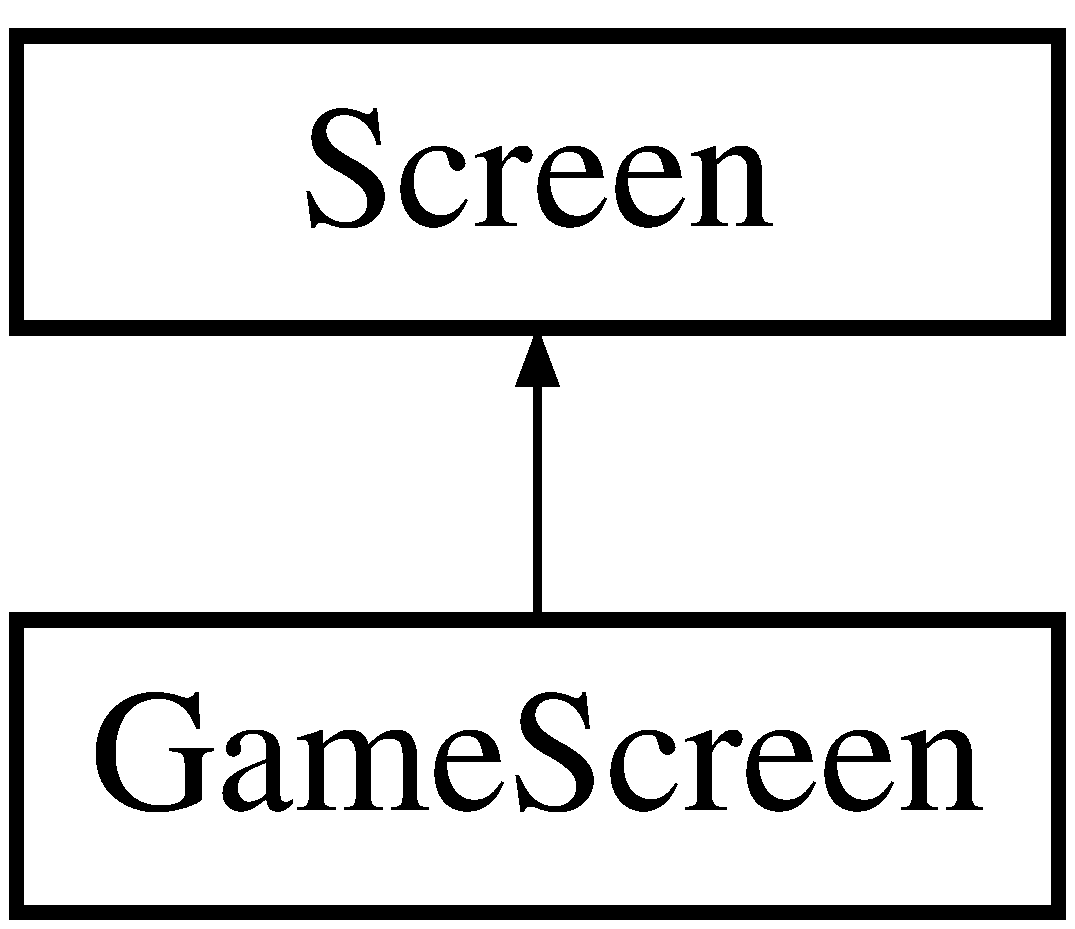
\includegraphics[height=2.000000cm]{classGameScreen}
\end{center}
\end{figure}
\subsection*{Public Member Functions}
\begin{DoxyCompactItemize}
\item 
void \hyperlink{classGameScreen_a2ca8233319e849881b40f6b51d70b5c2}{event\+Action} (A\+L\+L\+E\+G\+R\+O\+\_\+\+E\+V\+E\+NT \&, \hyperlink{classViewManager}{View\+Manager} $\ast$, \hyperlink{classGame}{Game} $\ast$)
\item 
void \hyperlink{classGameScreen_a1f82a990e5a99b6277d61a241f7ee249}{update\+Screen\+After\+Display\+Changes} ()
\item 
void \hyperlink{classGameScreen_a5dc1384fa03aa108acb594a25a37c6d3}{initialize\+Screen\+Elements} ()
\item 
std\+::string \hyperlink{classGameScreen_aed6639510a63371edde3c02b8772e965}{get\+Title} ()
\item 
{\bfseries Game\+Screen} (std\+::string, \hyperlink{classDisplay}{Display} $\ast$display)\hypertarget{classGameScreen_a938d3b8dcd74d5581bce846100893d65}{}\label{classGameScreen_a938d3b8dcd74d5581bce846100893d65}

\item 
void {\bfseries create\+Image} (Actor\+Id id, std\+::string path)\hypertarget{classGameScreen_abeea653575bf8c23ba338e4825ddfceb}{}\label{classGameScreen_abeea653575bf8c23ba338e4825ddfceb}

\item 
void {\bfseries create\+Text} (Actor\+Id id, std\+::string text)\hypertarget{classGameScreen_ae7bf62b6249da58e40dfffa4eb8d8bd9}{}\label{classGameScreen_ae7bf62b6249da58e40dfffa4eb8d8bd9}

\item 
void {\bfseries update\+Object} (Actor\+Id id, \hyperlink{classPoint}{Point} point, \hyperlink{classRotation}{Rotation} rotation, float zoom, std\+::string text)\hypertarget{classGameScreen_abd0496993fd77d75f51076fa4a4d73e3}{}\label{classGameScreen_abd0496993fd77d75f51076fa4a4d73e3}

\item 
void {\bfseries delete\+Object} (Actor\+Id id)\hypertarget{classGameScreen_ad352705fd0b44ec761149670e2b8d9f3}{}\label{classGameScreen_ad352705fd0b44ec761149670e2b8d9f3}

\item 
void {\bfseries refresh\+Screen} ()\hypertarget{classGameScreen_ac789a31dbf548073fc28753704ae8e92}{}\label{classGameScreen_ac789a31dbf548073fc28753704ae8e92}

\end{DoxyCompactItemize}


\subsection{Member Function Documentation}
\index{Game\+Screen@{Game\+Screen}!event\+Action@{event\+Action}}
\index{event\+Action@{event\+Action}!Game\+Screen@{Game\+Screen}}
\subsubsection[{\texorpdfstring{event\+Action(\+A\+L\+L\+E\+G\+R\+O\+\_\+\+E\+V\+E\+N\+T \&, View\+Manager $\ast$, Game $\ast$)}{eventAction(ALLEGRO_EVENT &, ViewManager *, Game *)}}]{\setlength{\rightskip}{0pt plus 5cm}void Game\+Screen\+::event\+Action (
\begin{DoxyParamCaption}
\item[{A\+L\+L\+E\+G\+R\+O\+\_\+\+E\+V\+E\+NT \&}]{ev, }
\item[{{\bf View\+Manager} $\ast$}]{vm, }
\item[{{\bf Game} $\ast$}]{g}
\end{DoxyParamCaption}
)\hspace{0.3cm}{\ttfamily [virtual]}}\hypertarget{classGameScreen_a2ca8233319e849881b40f6b51d70b5c2}{}\label{classGameScreen_a2ca8233319e849881b40f6b51d70b5c2}
Virtual method which does some actions when event occurs. 
\begin{DoxyParams}{Parameters}
{\em ev} & event which occured. \\
\hline
{\em vm} & pointer to the \hyperlink{classViewManager}{View\+Manager}. \\
\hline
{\em g} & pointer to the \hyperlink{classGame}{Game}. \\
\hline
\end{DoxyParams}


Reimplemented from \hyperlink{classScreen_a5fb59d03053c2d0aaca26f9480bbe433}{Screen}.

\index{Game\+Screen@{Game\+Screen}!get\+Title@{get\+Title}}
\index{get\+Title@{get\+Title}!Game\+Screen@{Game\+Screen}}
\subsubsection[{\texorpdfstring{get\+Title()}{getTitle()}}]{\setlength{\rightskip}{0pt plus 5cm}std\+::string Game\+Screen\+::get\+Title (
\begin{DoxyParamCaption}
{}
\end{DoxyParamCaption}
)\hspace{0.3cm}{\ttfamily [inline]}, {\ttfamily [virtual]}}\hypertarget{classGameScreen_aed6639510a63371edde3c02b8772e965}{}\label{classGameScreen_aed6639510a63371edde3c02b8772e965}
Returns \hyperlink{classScreen}{Screen} title (\hyperlink{classScreen}{Screen} titles are used to organize Screens). \begin{DoxyReturn}{Returns}
title of the screen. 
\end{DoxyReturn}


Reimplemented from \hyperlink{classScreen_a28df2a95a64693e2e5b1238c07c92115}{Screen}.

\index{Game\+Screen@{Game\+Screen}!initialize\+Screen\+Elements@{initialize\+Screen\+Elements}}
\index{initialize\+Screen\+Elements@{initialize\+Screen\+Elements}!Game\+Screen@{Game\+Screen}}
\subsubsection[{\texorpdfstring{initialize\+Screen\+Elements()}{initializeScreenElements()}}]{\setlength{\rightskip}{0pt plus 5cm}void Game\+Screen\+::initialize\+Screen\+Elements (
\begin{DoxyParamCaption}
{}
\end{DoxyParamCaption}
)\hspace{0.3cm}{\ttfamily [virtual]}}\hypertarget{classGameScreen_a5dc1384fa03aa108acb594a25a37c6d3}{}\label{classGameScreen_a5dc1384fa03aa108acb594a25a37c6d3}
Virtual method which is used to initialize special elements added to the \hyperlink{classScreen}{Screen} before it will be used 

Reimplemented from \hyperlink{classScreen_a207320477f0e323dc4cd36dbd4706238}{Screen}.

\index{Game\+Screen@{Game\+Screen}!update\+Screen\+After\+Display\+Changes@{update\+Screen\+After\+Display\+Changes}}
\index{update\+Screen\+After\+Display\+Changes@{update\+Screen\+After\+Display\+Changes}!Game\+Screen@{Game\+Screen}}
\subsubsection[{\texorpdfstring{update\+Screen\+After\+Display\+Changes()}{updateScreenAfterDisplayChanges()}}]{\setlength{\rightskip}{0pt plus 5cm}void Game\+Screen\+::update\+Screen\+After\+Display\+Changes (
\begin{DoxyParamCaption}
{}
\end{DoxyParamCaption}
)\hspace{0.3cm}{\ttfamily [virtual]}}\hypertarget{classGameScreen_a1f82a990e5a99b6277d61a241f7ee249}{}\label{classGameScreen_a1f82a990e5a99b6277d61a241f7ee249}
Let\textquotesingle{}s the \hyperlink{classScreen}{Screen} to change it\textquotesingle{}s objects after changes in the display (like resolution). 

Reimplemented from \hyperlink{classScreen_a0d283acd7432bd4fedd35cd147bdf4a8}{Screen}.



The documentation for this class was generated from the following files\+:\begin{DoxyCompactItemize}
\item 
src/\+View/Game\+Screen.\+h\item 
src/\+View/Game\+Screen.\+cpp\end{DoxyCompactItemize}

\hypertarget{classGameScreenEventInterpreter}{}\section{Game\+Screen\+Event\+Interpreter Class Reference}
\label{classGameScreenEventInterpreter}\index{Game\+Screen\+Event\+Interpreter@{Game\+Screen\+Event\+Interpreter}}
Inheritance diagram for Game\+Screen\+Event\+Interpreter\+:\begin{figure}[H]
\begin{center}
\leavevmode
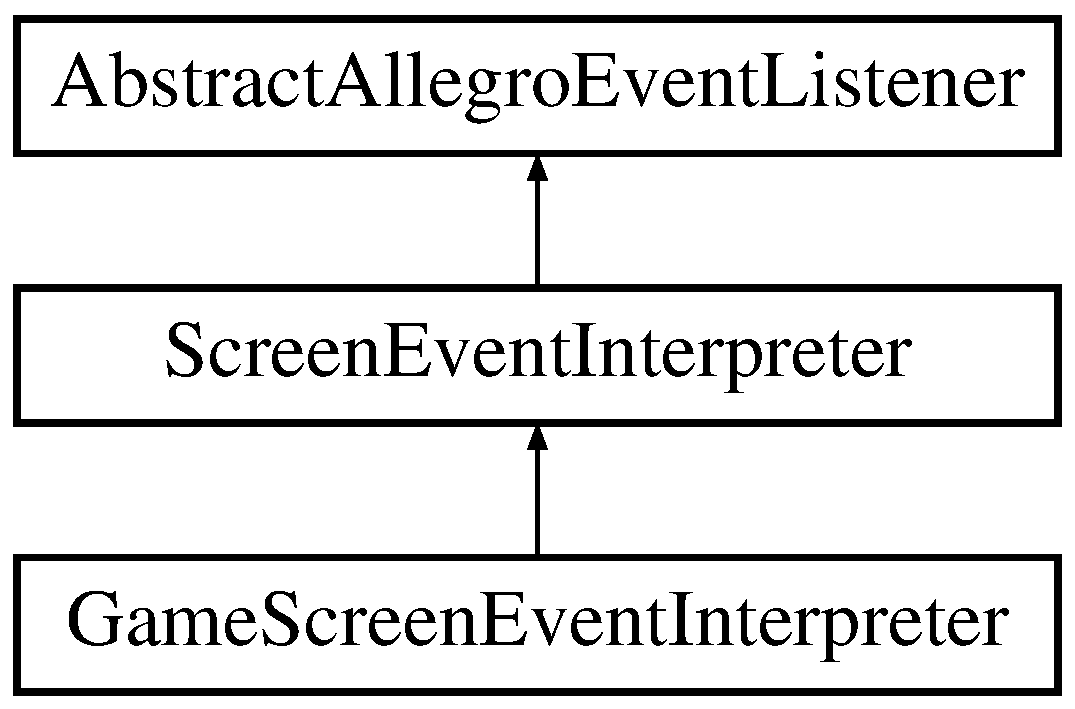
\includegraphics[height=3.000000cm]{classGameScreenEventInterpreter}
\end{center}
\end{figure}
\subsection*{Public Member Functions}
\begin{DoxyCompactItemize}
\item 
{\bfseries Game\+Screen\+Event\+Interpreter} (\hyperlink{classAllegroToGameKeyMapper}{Allegro\+To\+Game\+Key\+Mapper} \&key\+Mapper, \hyperlink{classMousePositionFetcher}{Mouse\+Position\+Fetcher} \&mouse\+Position\+Fetcher, \hyperlink{classGameScreen}{Game\+Screen} $\ast$game\+Screen, \hyperlink{classImageDataContainer}{Image\+Data\+Container} \&image\+Data\+Container, \hyperlink{classGame}{Game} \&game, \hyperlink{classScreenSize}{Screen\+Size} \&screen\+Size, \hyperlink{classSoundModule}{Sound\+Module} \&sound\+Module)\hypertarget{classGameScreenEventInterpreter_ae0b336acc8050ff68449dbf38f974bca}{}\label{classGameScreenEventInterpreter_ae0b336acc8050ff68449dbf38f974bca}

\item 
virtual void {\bfseries key\+Down} (int keynum)\hypertarget{classGameScreenEventInterpreter_a651b8768c75478fa88a5528bf1fe8a1e}{}\label{classGameScreenEventInterpreter_a651b8768c75478fa88a5528bf1fe8a1e}

\item 
virtual void {\bfseries time\+Event} ()\hypertarget{classGameScreenEventInterpreter_a1ac9277ffbcbbce67e6482a9f58f0648}{}\label{classGameScreenEventInterpreter_a1ac9277ffbcbbce67e6482a9f58f0648}

\item 
virtual std\+::string {\bfseries get\+Screen\+Name} ()\hypertarget{classGameScreenEventInterpreter_aa23b48d1b4f96bb1ad1b8a0adb42bf0f}{}\label{classGameScreenEventInterpreter_aa23b48d1b4f96bb1ad1b8a0adb42bf0f}

\end{DoxyCompactItemize}
\subsection*{Additional Inherited Members}


The documentation for this class was generated from the following files\+:\begin{DoxyCompactItemize}
\item 
src/\+Controller/Game\+Screen\+Event\+Interpreter.\+h\item 
src/\+Controller/Game\+Screen\+Event\+Interpreter.\+cpp\end{DoxyCompactItemize}

\hypertarget{classGameStopService}{}\section{Game\+Stop\+Service Class Reference}
\label{classGameStopService}\index{Game\+Stop\+Service@{Game\+Stop\+Service}}
Inheritance diagram for Game\+Stop\+Service\+:\begin{figure}[H]
\begin{center}
\leavevmode
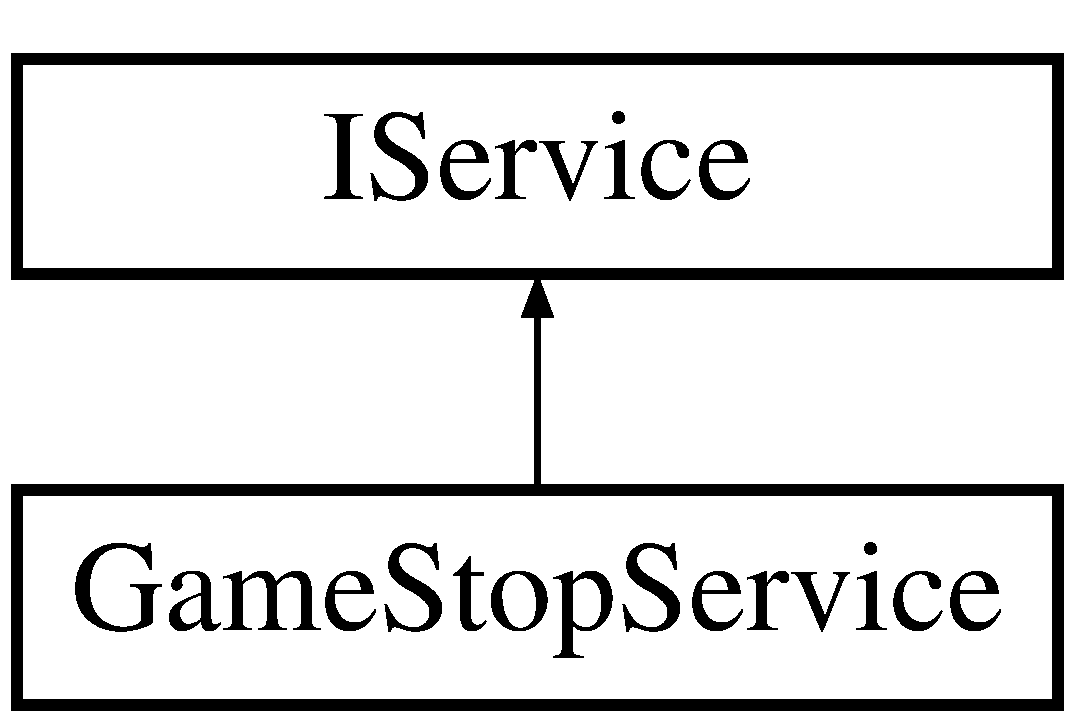
\includegraphics[height=2.000000cm]{classGameStopService}
\end{center}
\end{figure}
\subsection*{Public Member Functions}
\begin{DoxyCompactItemize}
\item 
{\bfseries Game\+Stop\+Service} (\hyperlink{classPythonModule}{Python\+Module} \&python\+\_\+, const std\+::shared\+\_\+ptr$<$ \hyperlink{classGameTimeProvider}{Game\+Time\+Provider} $>$ game\+Time\+Provider\+\_\+, const std\+::shared\+\_\+ptr$<$ \hyperlink{classBox2DService}{Box2\+D\+Service} $>$ box2d\+Service\+\_\+, std\+::shared\+\_\+ptr$<$ \hyperlink{classInputStateManager}{Input\+State\+Manager} $>$ input\+Manager)\hypertarget{classGameStopService_af17fa924810d813d0f542239f6e84ebe}{}\label{classGameStopService_af17fa924810d813d0f542239f6e84ebe}

\item 
void {\bfseries On\+Update} ()\hypertarget{classGameStopService_a8a6a9b15fc8984ad0196781f0c177188}{}\label{classGameStopService_a8a6a9b15fc8984ad0196781f0c177188}

\item 
void {\bfseries stop\+Game} ()\hypertarget{classGameStopService_ab66aee8a96a4758ee1ff2df32606420e}{}\label{classGameStopService_ab66aee8a96a4758ee1ff2df32606420e}

\item 
void {\bfseries start\+Game} ()\hypertarget{classGameStopService_a7b42f3c27d5d707468f42f143da5e9ce}{}\label{classGameStopService_a7b42f3c27d5d707468f42f143da5e9ce}

\end{DoxyCompactItemize}


The documentation for this class was generated from the following files\+:\begin{DoxyCompactItemize}
\item 
src/\+Model/\+Services/Game\+Stop\+Service.\+h\item 
src/\+Model/\+Services/Game\+Stop\+Service.\+cpp\end{DoxyCompactItemize}

\hypertarget{classGameTimeProvider}{}\section{Game\+Time\+Provider Class Reference}
\label{classGameTimeProvider}\index{Game\+Time\+Provider@{Game\+Time\+Provider}}
Inheritance diagram for Game\+Time\+Provider\+:\begin{figure}[H]
\begin{center}
\leavevmode
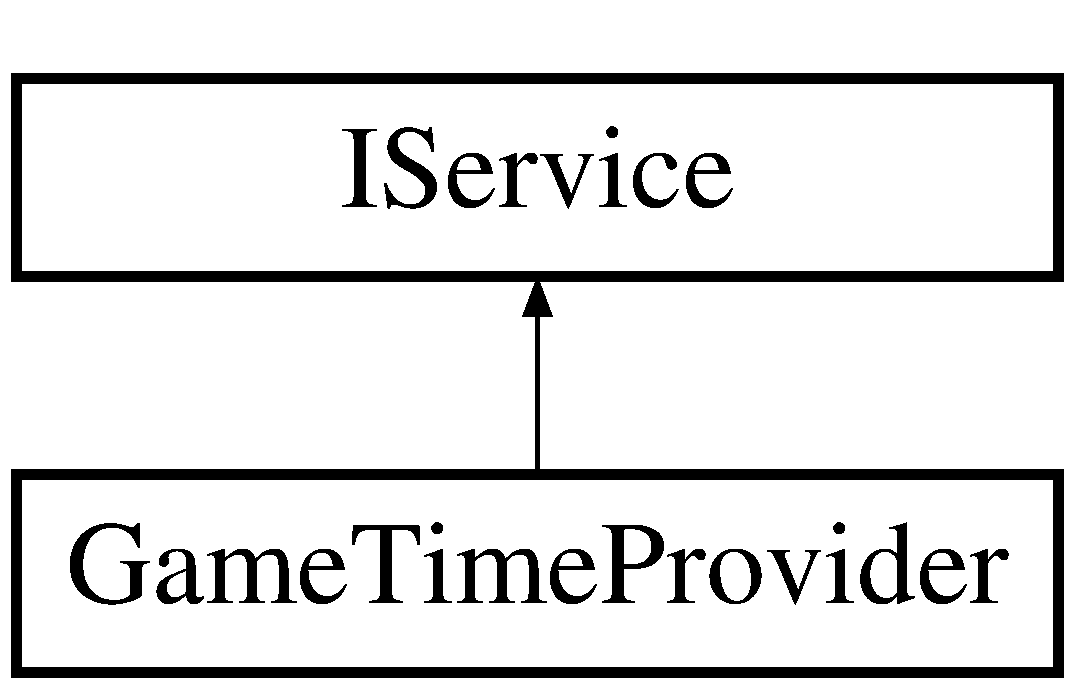
\includegraphics[height=2.000000cm]{classGameTimeProvider}
\end{center}
\end{figure}
\subsection*{Public Member Functions}
\begin{DoxyCompactItemize}
\item 
virtual void {\bfseries On\+Start} ()\hypertarget{classGameTimeProvider_a40ab7efa253a43e6a89ef4da6301d9ca}{}\label{classGameTimeProvider_a40ab7efa253a43e6a89ef4da6301d9ca}

\item 
virtual void {\bfseries On\+Update} ()\hypertarget{classGameTimeProvider_a9c90c29786e57ce72d6ba2e3c9ff9aec}{}\label{classGameTimeProvider_a9c90c29786e57ce72d6ba2e3c9ff9aec}

\item 
long {\bfseries get\+Miliseconds\+Since\+Game\+Start} ()\hypertarget{classGameTimeProvider_af995dede8e21de41a47e8db364531e8b}{}\label{classGameTimeProvider_af995dede8e21de41a47e8db364531e8b}

\item 
long {\bfseries get\+Miliseconds\+Between\+Frames} ()\hypertarget{classGameTimeProvider_a243a98c22d23c17691dab197c23574d6}{}\label{classGameTimeProvider_a243a98c22d23c17691dab197c23574d6}

\item 
void {\bfseries turn\+Off} ()\hypertarget{classGameTimeProvider_a8bc5613dac01d7d253050cadfb47dd5f}{}\label{classGameTimeProvider_a8bc5613dac01d7d253050cadfb47dd5f}

\item 
void {\bfseries turn\+On} ()\hypertarget{classGameTimeProvider_a4120c096bdd6112e90fdc7ea8eac1d43}{}\label{classGameTimeProvider_a4120c096bdd6112e90fdc7ea8eac1d43}

\end{DoxyCompactItemize}


The documentation for this class was generated from the following files\+:\begin{DoxyCompactItemize}
\item 
src/\+Model/\+Services/Game\+Time\+Provider.\+h\item 
src/\+Model/\+Services/Game\+Time\+Provider.\+cpp\end{DoxyCompactItemize}

\hypertarget{classGameTimeProviderTest}{}\section{Game\+Time\+Provider\+Test Class Reference}
\label{classGameTimeProviderTest}\index{Game\+Time\+Provider\+Test@{Game\+Time\+Provider\+Test}}
Inheritance diagram for Game\+Time\+Provider\+Test\+:\begin{figure}[H]
\begin{center}
\leavevmode
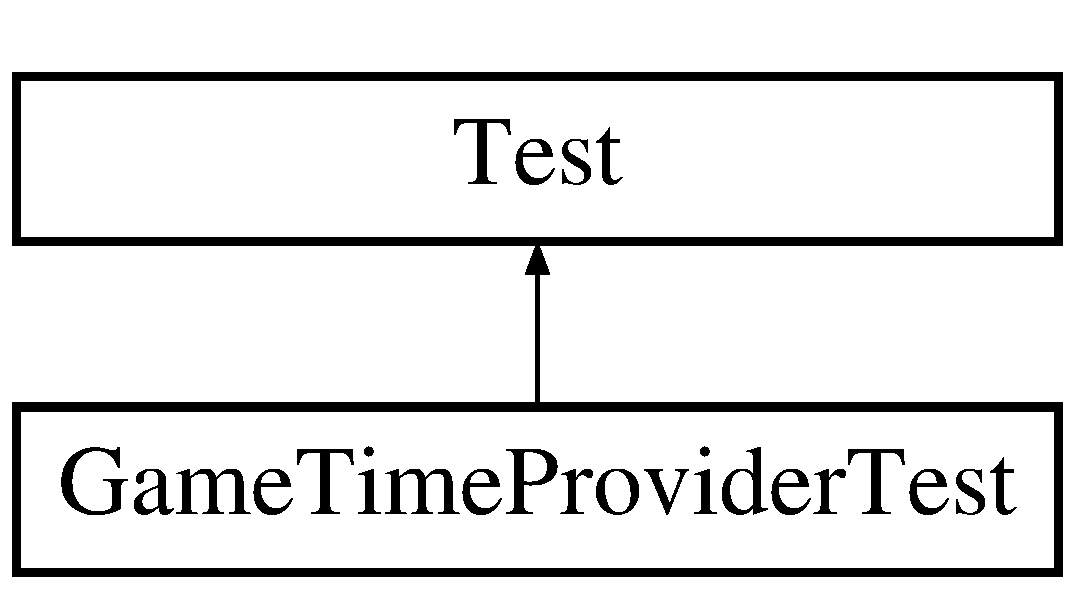
\includegraphics[height=2.000000cm]{classGameTimeProviderTest}
\end{center}
\end{figure}
\subsection*{Public Attributes}
\begin{DoxyCompactItemize}
\item 
int {\bfseries tolerable\+Diffrence\+In\+Miliseconds} = 4\hypertarget{classGameTimeProviderTest_a026ae8389cb9e4567c20c0ef975ca824}{}\label{classGameTimeProviderTest_a026ae8389cb9e4567c20c0ef975ca824}

\end{DoxyCompactItemize}


The documentation for this class was generated from the following file\+:\begin{DoxyCompactItemize}
\item 
test/\+Services/Game\+Time\+Provider\+Test.\+cpp\end{DoxyCompactItemize}

\hypertarget{classHealthPowerupCollisionComponent}{}\section{Health\+Powerup\+Collision\+Component Class Reference}
\label{classHealthPowerupCollisionComponent}\index{Health\+Powerup\+Collision\+Component@{Health\+Powerup\+Collision\+Component}}
Inheritance diagram for Health\+Powerup\+Collision\+Component\+:\begin{figure}[H]
\begin{center}
\leavevmode
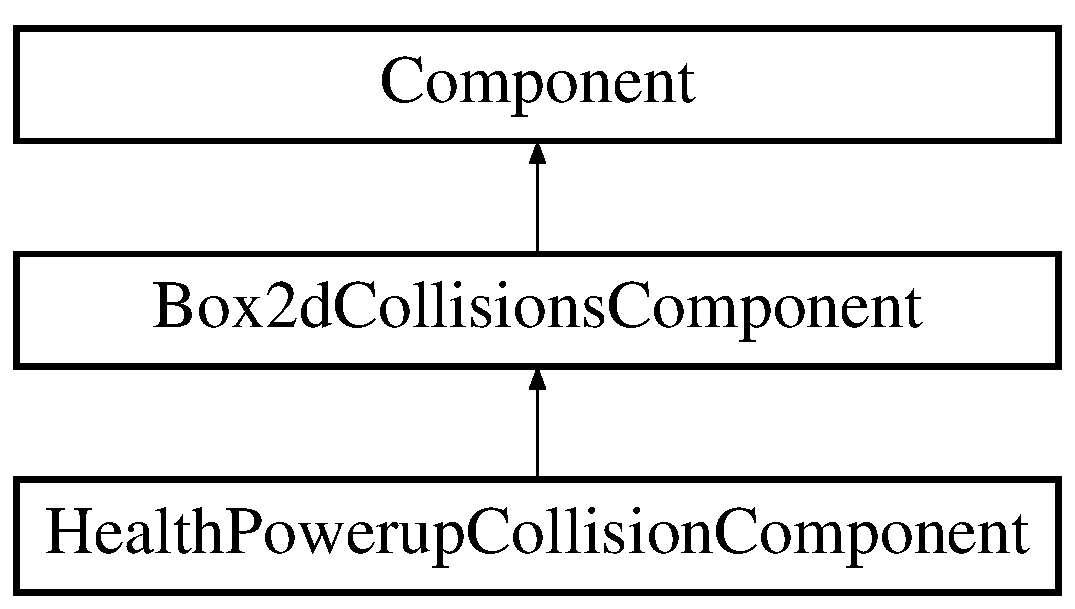
\includegraphics[height=3.000000cm]{classHealthPowerupCollisionComponent}
\end{center}
\end{figure}
\subsection*{Public Member Functions}
\begin{DoxyCompactItemize}
\item 
{\bfseries Health\+Powerup\+Collision\+Component} (\hyperlink{classContactComponentsContainer}{Contact\+Components\+Container} \&contact\+Container, std\+::shared\+\_\+ptr$<$ \hyperlink{classActorsContainer}{Actors\+Container} $>$ actors\+Container\+\_\+, std\+::shared\+\_\+ptr$<$ \hyperlink{classMusicManager}{Music\+Manager} $>$ music\+Manager\+\_\+, \hyperlink{classRocketLife}{Rocket\+Life} \&rocket\+Life)\hypertarget{classHealthPowerupCollisionComponent_a84287dd35e8bcfe39803fb31ffee3d2c}{}\label{classHealthPowerupCollisionComponent_a84287dd35e8bcfe39803fb31ffee3d2c}

\item 
void {\bfseries On\+Start} (\hyperlink{classIActor}{I\+Actor} \&actor)\hypertarget{classHealthPowerupCollisionComponent_a725faf63e859ed147aa0d5f020d24669}{}\label{classHealthPowerupCollisionComponent_a725faf63e859ed147aa0d5f020d24669}

\item 
bool {\bfseries manage\+Collision} (\hyperlink{structCollisionData}{Collision\+Data} \&data)\hypertarget{classHealthPowerupCollisionComponent_a602eab6b9e69a0c7c0ffa49dbd552075}{}\label{classHealthPowerupCollisionComponent_a602eab6b9e69a0c7c0ffa49dbd552075}

\end{DoxyCompactItemize}
\subsection*{Additional Inherited Members}


The documentation for this class was generated from the following files\+:\begin{DoxyCompactItemize}
\item 
src/\+Model/\+Actors/powerup/Health\+Powerup\+Collision\+Component.\+h\item 
src/\+Model/\+Actors/powerup/Health\+Powerup\+Collision\+Component.\+cpp\end{DoxyCompactItemize}

\hypertarget{classIActor}{}\section{I\+Actor Class Reference}
\label{classIActor}\index{I\+Actor@{I\+Actor}}
Inheritance diagram for I\+Actor\+:\begin{figure}[H]
\begin{center}
\leavevmode
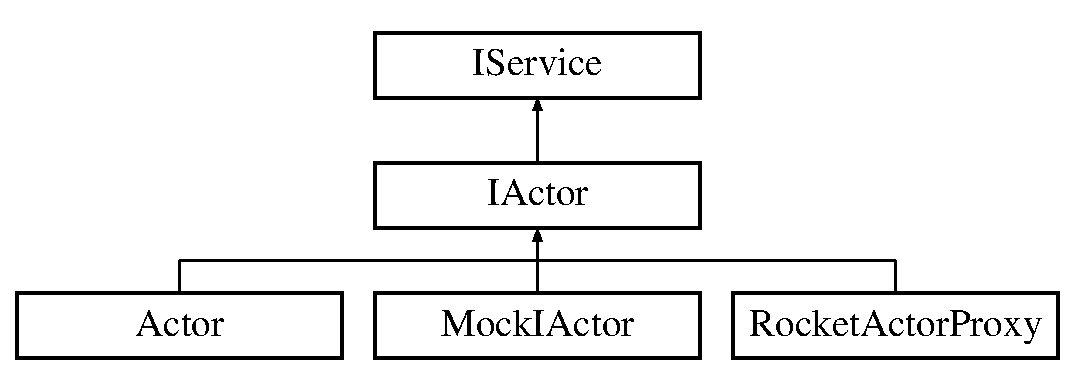
\includegraphics[height=3.000000cm]{classIActor}
\end{center}
\end{figure}
\subsection*{Public Member Functions}
\begin{DoxyCompactItemize}
\item 
virtual void {\bfseries add\+Component} (std\+::shared\+\_\+ptr$<$ \hyperlink{classComponent}{Component} $>$ component)=0\hypertarget{classIActor_a406c89af95f0c6abf42b3ac07a15dd08}{}\label{classIActor_a406c89af95f0c6abf42b3ac07a15dd08}

\item 
virtual void {\bfseries remove\+Component} (\hyperlink{classComponent}{Component} $\ast$component\+To\+Delete)=0\hypertarget{classIActor_a75401386ddb0b7bec49d1f5b3c9d137c}{}\label{classIActor_a75401386ddb0b7bec49d1f5b3c9d137c}

\item 
{\footnotesize template$<$typename Component\+Type $>$ }\\std\+::shared\+\_\+ptr$<$ Component\+Type $>$ {\bfseries get\+Only\+Component} ()\hypertarget{classIActor_a096d0f46b11274b8e0154080b18c5ea4}{}\label{classIActor_a096d0f46b11274b8e0154080b18c5ea4}

\item 
{\footnotesize template$<$typename Component\+Type $>$ }\\bool {\bfseries is\+Component\+Present} ()\hypertarget{classIActor_a47e7c67883c9207eb2080a4c6aa9c100}{}\label{classIActor_a47e7c67883c9207eb2080a4c6aa9c100}

\item 
virtual Actor\+Id {\bfseries get\+Actor\+Id} () const  =0\hypertarget{classIActor_a5a7d30292e74b082145ab74320fae7e5}{}\label{classIActor_a5a7d30292e74b082145ab74320fae7e5}

\item 
virtual std\+::shared\+\_\+ptr$<$ \hyperlink{classComponent}{Component} $>$ {\bfseries get\+Only\+Component} (\hyperlink{classComponentTypeChecker}{Component\+Type\+Checker} checker)=0\hypertarget{classIActor_ae363a172564fa4ed555e486fc4770350}{}\label{classIActor_ae363a172564fa4ed555e486fc4770350}

\item 
virtual bool {\bfseries is\+Component\+Present} (\hyperlink{classComponentTypeChecker}{Component\+Type\+Checker} checker)=0\hypertarget{classIActor_a31d4e5d91cf2ec4c6a8fff033a04290c}{}\label{classIActor_a31d4e5d91cf2ec4c6a8fff033a04290c}

\end{DoxyCompactItemize}


The documentation for this class was generated from the following file\+:\begin{DoxyCompactItemize}
\item 
src/\+Model/\+Actors/I\+Actor.\+h\end{DoxyCompactItemize}

\hypertarget{classIBorderIndicatorPositionProvider}{}\section{I\+Border\+Indicator\+Position\+Provider Class Reference}
\label{classIBorderIndicatorPositionProvider}\index{I\+Border\+Indicator\+Position\+Provider@{I\+Border\+Indicator\+Position\+Provider}}
Inheritance diagram for I\+Border\+Indicator\+Position\+Provider\+:\begin{figure}[H]
\begin{center}
\leavevmode
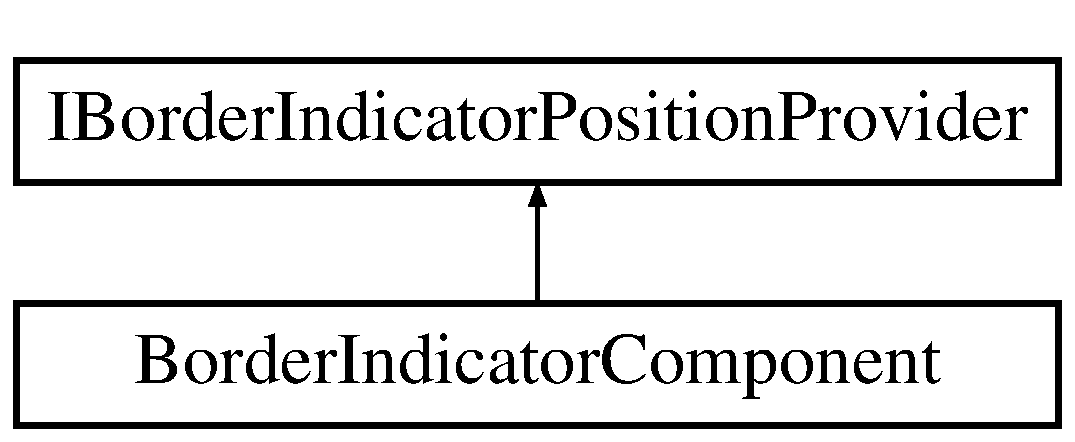
\includegraphics[height=2.000000cm]{classIBorderIndicatorPositionProvider}
\end{center}
\end{figure}
\subsection*{Public Member Functions}
\begin{DoxyCompactItemize}
\item 
virtual \hyperlink{classPoint}{Point} {\bfseries get\+Border\+Indicator\+Position} ()=0\hypertarget{classIBorderIndicatorPositionProvider_a3a86830892aae80b3fcab12fb5f9dec3}{}\label{classIBorderIndicatorPositionProvider_a3a86830892aae80b3fcab12fb5f9dec3}

\end{DoxyCompactItemize}


The documentation for this class was generated from the following file\+:\begin{DoxyCompactItemize}
\item 
src/\+Model/\+Actors/second\+Player/I\+Border\+Indicator\+Position\+Provider.\+h\end{DoxyCompactItemize}

\hypertarget{classIBox2dComponent}{}\section{I\+Box2d\+Component Class Reference}
\label{classIBox2dComponent}\index{I\+Box2d\+Component@{I\+Box2d\+Component}}
Inheritance diagram for I\+Box2d\+Component\+:\begin{figure}[H]
\begin{center}
\leavevmode
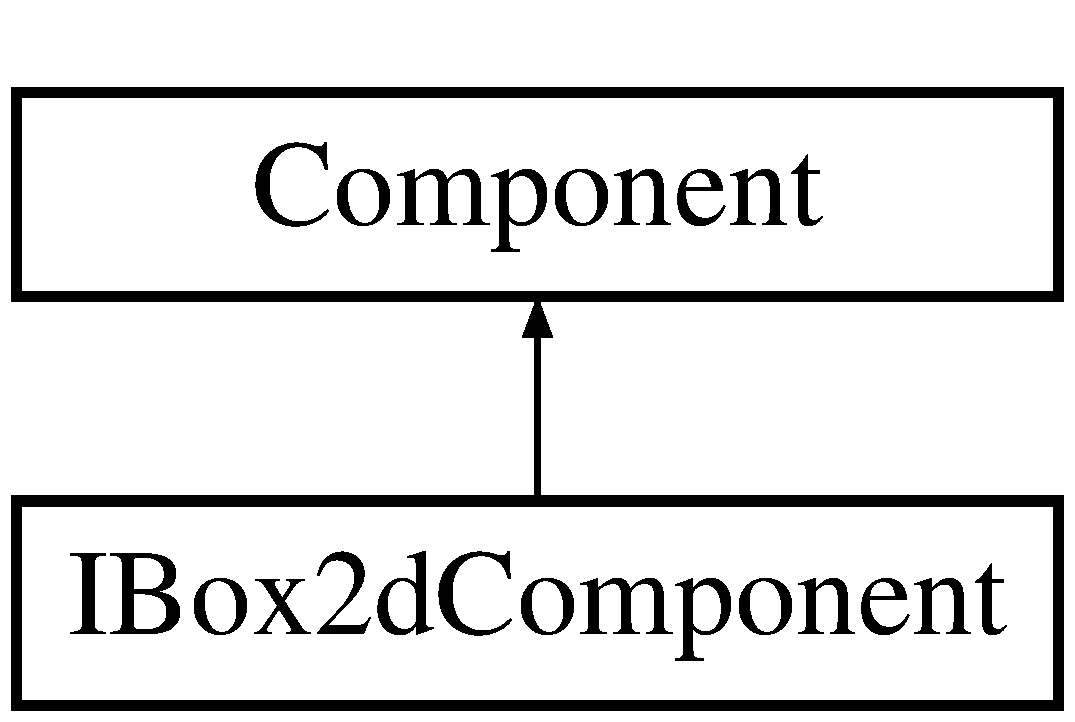
\includegraphics[height=2.000000cm]{classIBox2dComponent}
\end{center}
\end{figure}
\subsection*{Public Member Functions}
\begin{DoxyCompactItemize}
\item 
virtual void {\bfseries set\+Position} (double x, double y)=0\hypertarget{classIBox2dComponent_a2a65930e3f85605da4cbc31106b42f2c}{}\label{classIBox2dComponent_a2a65930e3f85605da4cbc31106b42f2c}

\item 
virtual void {\bfseries set\+Rotation} (double rotation)=0\hypertarget{classIBox2dComponent_a0b5f76bd2ba3314ff28ddd0c687c8263}{}\label{classIBox2dComponent_a0b5f76bd2ba3314ff28ddd0c687c8263}

\end{DoxyCompactItemize}


The documentation for this class was generated from the following file\+:\begin{DoxyCompactItemize}
\item 
src/\+Model/box2d/I\+Box2d\+Component.\+h\end{DoxyCompactItemize}

\hypertarget{classIDrawablePrimitive}{}\section{I\+Drawable\+Primitive Class Reference}
\label{classIDrawablePrimitive}\index{I\+Drawable\+Primitive@{I\+Drawable\+Primitive}}
Inheritance diagram for I\+Drawable\+Primitive\+:\begin{figure}[H]
\begin{center}
\leavevmode
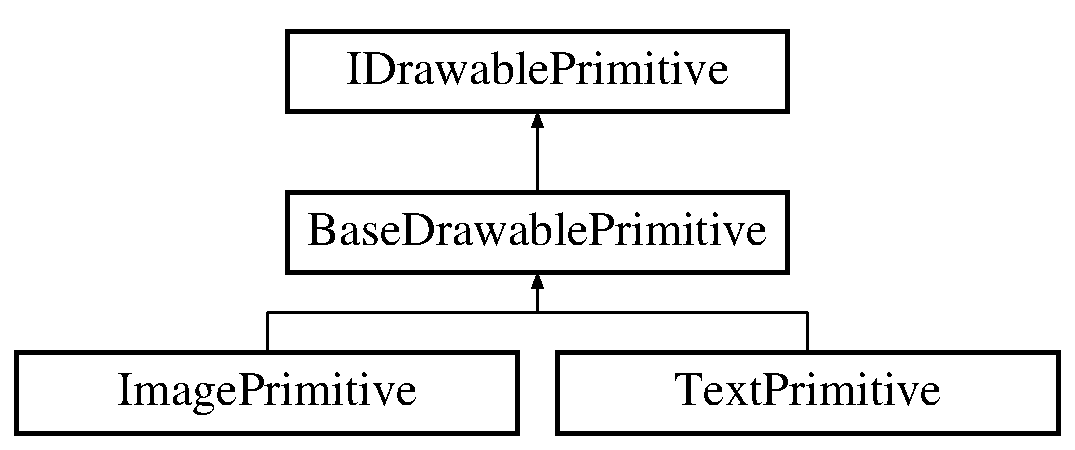
\includegraphics[height=3.000000cm]{classIDrawablePrimitive}
\end{center}
\end{figure}
\subsection*{Public Member Functions}
\begin{DoxyCompactItemize}
\item 
virtual \hyperlink{classPoint}{Point} {\bfseries get\+Position} () const  =0\hypertarget{classIDrawablePrimitive_a1366689d9e0fd0e45d24874bf945ef32}{}\label{classIDrawablePrimitive_a1366689d9e0fd0e45d24874bf945ef32}

\item 
virtual void {\bfseries set\+Position} (\hyperlink{classPoint}{Point} new\+Position)=0\hypertarget{classIDrawablePrimitive_a0e43fe084441b21ea58edd28c21dfe0a}{}\label{classIDrawablePrimitive_a0e43fe084441b21ea58edd28c21dfe0a}

\item 
virtual \hyperlink{classRotation}{Rotation} {\bfseries get\+Rotation} () const  =0\hypertarget{classIDrawablePrimitive_a4e43af39ac4628a12d92920f35837874}{}\label{classIDrawablePrimitive_a4e43af39ac4628a12d92920f35837874}

\item 
virtual void {\bfseries set\+Rotation} (\hyperlink{classRotation}{Rotation} rotation)=0\hypertarget{classIDrawablePrimitive_a393a9430549900e517dd0a69677a1be9}{}\label{classIDrawablePrimitive_a393a9430549900e517dd0a69677a1be9}

\item 
virtual \hyperlink{classScaleToScreen}{Scale\+To\+Screen} {\bfseries get\+Scale} () const  =0\hypertarget{classIDrawablePrimitive_aa76cf76b59dc423c4caa1bdaa76d7af7}{}\label{classIDrawablePrimitive_aa76cf76b59dc423c4caa1bdaa76d7af7}

\item 
virtual Actor\+Id {\bfseries get\+Actor\+Id} () const  =0\hypertarget{classIDrawablePrimitive_a233ea34c9d3467841407627457d2a705}{}\label{classIDrawablePrimitive_a233ea34c9d3467841407627457d2a705}

\item 
virtual void {\bfseries accept} (\hyperlink{classDrawablePrimitiveVisitor}{Drawable\+Primitive\+Visitor} \&visitor)=0\hypertarget{classIDrawablePrimitive_af245651a3f3887977a1a9db2f0cf62e8}{}\label{classIDrawablePrimitive_af245651a3f3887977a1a9db2f0cf62e8}

\end{DoxyCompactItemize}


The documentation for this class was generated from the following file\+:\begin{DoxyCompactItemize}
\item 
src/\+Model/\+Model\+Drawing/I\+Drawable\+Primitive.\+h\end{DoxyCompactItemize}

\hypertarget{classIDrawingSystem}{}\section{I\+Drawing\+System Class Reference}
\label{classIDrawingSystem}\index{I\+Drawing\+System@{I\+Drawing\+System}}
Inheritance diagram for I\+Drawing\+System\+:\begin{figure}[H]
\begin{center}
\leavevmode
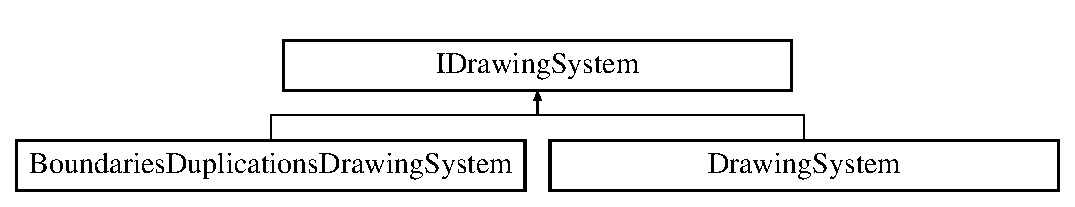
\includegraphics[height=2.000000cm]{classIDrawingSystem}
\end{center}
\end{figure}
\subsection*{Public Member Functions}
\begin{DoxyCompactItemize}
\item 
virtual void {\bfseries draw\+Image} (Image\+Primitive\+Type type, \hyperlink{classPoint}{Point} position, \hyperlink{classRotation}{Rotation} rotation, \hyperlink{classScaleToScreen}{Scale\+To\+Screen} scale, Actor\+Id actor\+Id)=0\hypertarget{classIDrawingSystem_ae4016831473bbdbc878adfd6f6907671}{}\label{classIDrawingSystem_ae4016831473bbdbc878adfd6f6907671}

\item 
virtual void {\bfseries draw\+Text} (std\+::string text\+Value, \hyperlink{classPoint}{Point} position, Actor\+Id actor\+Id)=0\hypertarget{classIDrawingSystem_a1729c24b624d76ac677e0b216215edb6}{}\label{classIDrawingSystem_a1729c24b624d76ac677e0b216215edb6}

\item 
virtual void {\bfseries add\+Removed\+Actor\+Id} (Actor\+Id id)=0\hypertarget{classIDrawingSystem_a179d95332581cf97996c8221e8813f1c}{}\label{classIDrawingSystem_a179d95332581cf97996c8221e8813f1c}

\end{DoxyCompactItemize}


The documentation for this class was generated from the following file\+:\begin{DoxyCompactItemize}
\item 
src/\+Model/\+Model\+Drawing/I\+Drawing\+System.\+h\end{DoxyCompactItemize}

\hypertarget{classIEndToEndExpectation}{}\section{I\+End\+To\+End\+Expectation Class Reference}
\label{classIEndToEndExpectation}\index{I\+End\+To\+End\+Expectation@{I\+End\+To\+End\+Expectation}}
Inheritance diagram for I\+End\+To\+End\+Expectation\+:\begin{figure}[H]
\begin{center}
\leavevmode
\includegraphics[height=0.653951cm]{classIEndToEndExpectation}
\end{center}
\end{figure}
\subsection*{Public Member Functions}
\begin{DoxyCompactItemize}
\item 
virtual std\+::string {\bfseries get\+Expectation\+Description} ()=0\hypertarget{classIEndToEndExpectation_a50719797f203d30987cc82835d6fc785}{}\label{classIEndToEndExpectation_a50719797f203d30987cc82835d6fc785}

\item 
virtual bool {\bfseries check\+Expectation} ()=0\hypertarget{classIEndToEndExpectation_afba5cd79bed75f29f6ed4a41f94ba8d0}{}\label{classIEndToEndExpectation_afba5cd79bed75f29f6ed4a41f94ba8d0}

\item 
virtual std\+::string {\bfseries get\+Failure\+Message} ()=0\hypertarget{classIEndToEndExpectation_a7efc089699c94cd9f3463363ff25f9b1}{}\label{classIEndToEndExpectation_a7efc089699c94cd9f3463363ff25f9b1}

\item 
virtual void {\bfseries before\+First\+Update} (std\+::shared\+\_\+ptr$<$ \hyperlink{classGame}{Game} $>$)\hypertarget{classIEndToEndExpectation_a74f22c283e4f7f3d41c2a0b612dab376}{}\label{classIEndToEndExpectation_a74f22c283e4f7f3d41c2a0b612dab376}

\end{DoxyCompactItemize}


The documentation for this class was generated from the following file\+:\begin{DoxyCompactItemize}
\item 
test/\+End\+To\+End\+Tests/expectations/I\+End\+To\+End\+Expectation.\+h\end{DoxyCompactItemize}

\hypertarget{classIInputStateGetter}{}\section{I\+Input\+State\+Getter Class Reference}
\label{classIInputStateGetter}\index{I\+Input\+State\+Getter@{I\+Input\+State\+Getter}}
Inheritance diagram for I\+Input\+State\+Getter\+:\begin{figure}[H]
\begin{center}
\leavevmode
\includegraphics[height=3.000000cm]{classIInputStateGetter}
\end{center}
\end{figure}
\subsection*{Public Member Functions}
\begin{DoxyCompactItemize}
\item 
virtual void {\bfseries game\+Key\+Is\+Pressed} (Keys key)=0\hypertarget{classIInputStateGetter_afe4c6eb4febc8aeca2734c36c397e0a2}{}\label{classIInputStateGetter_afe4c6eb4febc8aeca2734c36c397e0a2}

\item 
virtual void {\bfseries set\+Mouse\+Position} (double x, double y)=0\hypertarget{classIInputStateGetter_a51f4228098714ee3ac162966f702b561}{}\label{classIInputStateGetter_a51f4228098714ee3ac162966f702b561}

\end{DoxyCompactItemize}


The documentation for this class was generated from the following file\+:\begin{DoxyCompactItemize}
\item 
src/\+Model/model\+Interfaces/I\+Input\+State\+Getter.\+h\end{DoxyCompactItemize}

\hypertarget{classIInputStateProvider}{}\section{I\+Input\+State\+Provider Class Reference}
\label{classIInputStateProvider}\index{I\+Input\+State\+Provider@{I\+Input\+State\+Provider}}
Inheritance diagram for I\+Input\+State\+Provider\+:\begin{figure}[H]
\begin{center}
\leavevmode
\includegraphics[height=2.000000cm]{classIInputStateProvider}
\end{center}
\end{figure}
\subsection*{Public Member Functions}
\begin{DoxyCompactItemize}
\item 
virtual bool {\bfseries was\+Clicked} (Keys key)=0\hypertarget{classIInputStateProvider_a6c97f490d462dadd588acb63963c7f47}{}\label{classIInputStateProvider_a6c97f490d462dadd588acb63963c7f47}

\item 
virtual bool {\bfseries is\+Pressed} (Keys key)=0\hypertarget{classIInputStateProvider_a48b11ddcc2c98525b0815fcc0970439d}{}\label{classIInputStateProvider_a48b11ddcc2c98525b0815fcc0970439d}

\item 
virtual \hyperlink{classPoint}{Point} {\bfseries get\+Mouse\+Position} ()=0\hypertarget{classIInputStateProvider_a46d95d5517d1bef12b0820508d0bafed}{}\label{classIInputStateProvider_a46d95d5517d1bef12b0820508d0bafed}

\end{DoxyCompactItemize}


The documentation for this class was generated from the following file\+:\begin{DoxyCompactItemize}
\item 
src/\+Model/model\+Interfaces/I\+Input\+State\+Provider.\+h\end{DoxyCompactItemize}

\hypertarget{classIInPythonModule}{}\section{I\+In\+Python\+Module Class Reference}
\label{classIInPythonModule}\index{I\+In\+Python\+Module@{I\+In\+Python\+Module}}
Inheritance diagram for I\+In\+Python\+Module\+:\begin{figure}[H]
\begin{center}
\leavevmode
\includegraphics[height=2.000000cm]{classIInPythonModule}
\end{center}
\end{figure}
\subsection*{Public Member Functions}
\begin{DoxyCompactItemize}
\item 
virtual void {\bfseries add\+Command} (std\+::string command\+Text)=0\hypertarget{classIInPythonModule_a5139355410f82de6b0accdf6221e9522}{}\label{classIInPythonModule_a5139355410f82de6b0accdf6221e9522}

\end{DoxyCompactItemize}


The documentation for this class was generated from the following file\+:\begin{DoxyCompactItemize}
\item 
src/\+Model/python/I\+In\+Python\+Module.\+h\end{DoxyCompactItemize}

\hypertarget{structImageData}{}\section{Image\+Data Struct Reference}
\label{structImageData}\index{Image\+Data@{Image\+Data}}
\subsection*{Public Attributes}
\begin{DoxyCompactItemize}
\item 
unsigned int {\bfseries x\+Size}\hypertarget{structImageData_ae356932e0569700e204cd40eee304cb0}{}\label{structImageData_ae356932e0569700e204cd40eee304cb0}

\item 
unsigned int {\bfseries y\+Size}\hypertarget{structImageData_a983cd6be7a6728beec0c89d21c8ca3e4}{}\label{structImageData_a983cd6be7a6728beec0c89d21c8ca3e4}

\item 
const char $\ast$ {\bfseries path}\hypertarget{structImageData_abdf724335a32a9621a7f42612382bae3}{}\label{structImageData_abdf724335a32a9621a7f42612382bae3}

\end{DoxyCompactItemize}


The documentation for this struct was generated from the following file\+:\begin{DoxyCompactItemize}
\item 
src/\+View/Image\+Data.\+h\end{DoxyCompactItemize}

\hypertarget{classImageDataContainer}{}\section{Image\+Data\+Container Class Reference}
\label{classImageDataContainer}\index{Image\+Data\+Container@{Image\+Data\+Container}}
\subsection*{Public Member Functions}
\begin{DoxyCompactItemize}
\item 
void {\bfseries add\+Data} (Image\+Primitive\+Type type, \hyperlink{structImageData}{Image\+Data} data)\hypertarget{classImageDataContainer_ae2669ff38a90086bf00521cbe0ad5d14}{}\label{classImageDataContainer_ae2669ff38a90086bf00521cbe0ad5d14}

\item 
\hyperlink{structImageData}{Image\+Data} {\bfseries get\+Data} (Image\+Primitive\+Type type)\hypertarget{classImageDataContainer_a7ded5b1de74d09b4d0256f38a085cdc5}{}\label{classImageDataContainer_a7ded5b1de74d09b4d0256f38a085cdc5}

\item 
std\+::map$<$ Image\+Primitive\+Type, \hyperlink{classPoint}{Point} $>$ {\bfseries get\+Image\+Sizes\+Map} (double scaling\+Factor)\hypertarget{classImageDataContainer_a2ced17bbba9e5864ad621d74fdce3b2a}{}\label{classImageDataContainer_a2ced17bbba9e5864ad621d74fdce3b2a}

\end{DoxyCompactItemize}


The documentation for this class was generated from the following files\+:\begin{DoxyCompactItemize}
\item 
src/\+Controller/Image\+Data\+Container.\+h\item 
src/\+Controller/Image\+Data\+Container.\+cpp\end{DoxyCompactItemize}

\hypertarget{classImagePrimitive}{}\section{Image\+Primitive Class Reference}
\label{classImagePrimitive}\index{Image\+Primitive@{Image\+Primitive}}
Inheritance diagram for Image\+Primitive\+:\begin{figure}[H]
\begin{center}
\leavevmode
\includegraphics[height=3.000000cm]{classImagePrimitive}
\end{center}
\end{figure}
\subsection*{Public Member Functions}
\begin{DoxyCompactItemize}
\item 
{\bfseries Image\+Primitive} (const \hyperlink{classPoint}{Point} \&position\+\_\+, const \hyperlink{classRotation}{Rotation} \&rotation\+\_\+, const \hyperlink{classScaleToScreen}{Scale\+To\+Screen} \&scale\+\_\+, const Actor\+Id \&id, const Image\+Primitive\+Type \&image\+Type\+\_\+)\hypertarget{classImagePrimitive_a0d35b1b34707ccb99a843fe7cf0681af}{}\label{classImagePrimitive_a0d35b1b34707ccb99a843fe7cf0681af}

\item 
Image\+Primitive\+Type {\bfseries get\+Image\+Type} () const \hypertarget{classImagePrimitive_ac2ac781665a5eedbdf3dba72c98abe81}{}\label{classImagePrimitive_ac2ac781665a5eedbdf3dba72c98abe81}

\item 
virtual void {\bfseries accept} (\hyperlink{classDrawablePrimitiveVisitor}{Drawable\+Primitive\+Visitor} \&visitor) override\hypertarget{classImagePrimitive_a5ae2d03cfafb4ff31d7cefef197c142d}{}\label{classImagePrimitive_a5ae2d03cfafb4ff31d7cefef197c142d}

\end{DoxyCompactItemize}


The documentation for this class was generated from the following files\+:\begin{DoxyCompactItemize}
\item 
src/\+Model/\+Model\+Drawing/Image\+Primitive.\+h\item 
src/\+Model/\+Model\+Drawing/Image\+Primitive.\+cpp\end{DoxyCompactItemize}

\hypertarget{classImagePrimitiveExpectation}{}\section{Image\+Primitive\+Expectation Class Reference}
\label{classImagePrimitiveExpectation}\index{Image\+Primitive\+Expectation@{Image\+Primitive\+Expectation}}
Inheritance diagram for Image\+Primitive\+Expectation\+:\begin{figure}[H]
\begin{center}
\leavevmode
\includegraphics[height=2.000000cm]{classImagePrimitiveExpectation}
\end{center}
\end{figure}
\subsection*{Public Member Functions}
\begin{DoxyCompactItemize}
\item 
{\bfseries Image\+Primitive\+Expectation} (std\+::function$<$ bool(\hyperlink{classImagePrimitive}{Image\+Primitive} \&)$>$ primitives\+Selecting\+Function, std\+::function$<$ void(\hyperlink{classImagePrimitive}{Image\+Primitive} \&)$>$ primitives\+Assertion\+Function)\hypertarget{classImagePrimitiveExpectation_aef3b5e728dc3bba87240c6973d3ba364}{}\label{classImagePrimitiveExpectation_aef3b5e728dc3bba87240c6973d3ba364}

\item 
virtual std\+::string {\bfseries get\+Expectation\+Description} ()\hypertarget{classImagePrimitiveExpectation_ae57ed7b9198d2b1e8f203e853decf1c9}{}\label{classImagePrimitiveExpectation_ae57ed7b9198d2b1e8f203e853decf1c9}

\item 
virtual bool {\bfseries check\+Expectation} ()\hypertarget{classImagePrimitiveExpectation_a6a6c79f8cef08b81b61632e20e2ffc0e}{}\label{classImagePrimitiveExpectation_a6a6c79f8cef08b81b61632e20e2ffc0e}

\item 
virtual std\+::string {\bfseries get\+Failure\+Message} ()\hypertarget{classImagePrimitiveExpectation_a523380f8b393b8e2e8054c1c746b46f8}{}\label{classImagePrimitiveExpectation_a523380f8b393b8e2e8054c1c746b46f8}

\item 
virtual void {\bfseries before\+First\+Update} (std\+::shared\+\_\+ptr$<$ \hyperlink{classGame}{Game} $>$ g)\hypertarget{classImagePrimitiveExpectation_a84bde7866ee1c0f086db3511ebe752b3}{}\label{classImagePrimitiveExpectation_a84bde7866ee1c0f086db3511ebe752b3}

\end{DoxyCompactItemize}


The documentation for this class was generated from the following files\+:\begin{DoxyCompactItemize}
\item 
test/\+End\+To\+End\+Tests/expectations/Image\+Primitive\+Expectation.\+h\item 
test/\+End\+To\+End\+Tests/expectations/Image\+Primitive\+Expectation.\+cpp\end{DoxyCompactItemize}

\hypertarget{classImageScalesContainer}{}\section{Image\+Scales\+Container Class Reference}
\label{classImageScalesContainer}\index{Image\+Scales\+Container@{Image\+Scales\+Container}}
\subsection*{Public Member Functions}
\begin{DoxyCompactItemize}
\item 
{\bfseries Image\+Scales\+Container} (\hyperlink{classGameConfiguration}{Game\+Configuration} \&game\+Configuration\+\_\+, const std\+::map$<$ Image\+Primitive\+Type, \hyperlink{classPoint}{Point} $>$ \&image\+Primitives\+Size\+Map\+\_\+)\hypertarget{classImageScalesContainer_a7b3dabbfeb70082e1b54ab0f34344380}{}\label{classImageScalesContainer_a7b3dabbfeb70082e1b54ab0f34344380}

\item 
\hyperlink{classScaleToScreen}{Scale\+To\+Screen} {\bfseries get\+Image\+Scale} (Image\+Primitive\+Type type)\hypertarget{classImageScalesContainer_ade2c65ef2528b5354906f8e5625a12d6}{}\label{classImageScalesContainer_ade2c65ef2528b5354906f8e5625a12d6}

\item 
\hyperlink{classPoint}{Point} {\bfseries get\+Screen\+Size} ()\hypertarget{classImageScalesContainer_a93cf314cbc3a2230120799f7a68f5353}{}\label{classImageScalesContainer_a93cf314cbc3a2230120799f7a68f5353}

\end{DoxyCompactItemize}


The documentation for this class was generated from the following file\+:\begin{DoxyCompactItemize}
\item 
src/\+Model/\+Model\+Drawing/Image\+Scales\+Container.\+h\end{DoxyCompactItemize}

\hypertarget{classInitialRocketSettings}{}\section{Initial\+Rocket\+Settings Class Reference}
\label{classInitialRocketSettings}\index{Initial\+Rocket\+Settings@{Initial\+Rocket\+Settings}}
\subsection*{Static Public Member Functions}
\begin{DoxyCompactItemize}
\item 
static \hyperlink{classPoint}{Point} {\bfseries initial\+Position} ()\hypertarget{classInitialRocketSettings_a7b3067d1d07083b451545bd837ef6e2d}{}\label{classInitialRocketSettings_a7b3067d1d07083b451545bd837ef6e2d}

\item 
static \hyperlink{classRotation}{Rotation} {\bfseries initial\+Rotation} ()\hypertarget{classInitialRocketSettings_a00643433517033fd4dbaa6bd3f9bbf5f}{}\label{classInitialRocketSettings_a00643433517033fd4dbaa6bd3f9bbf5f}

\end{DoxyCompactItemize}


The documentation for this class was generated from the following files\+:\begin{DoxyCompactItemize}
\item 
src/\+Model/\+Actors/\+Rocket/Initial\+Rocket\+Settings.\+h\item 
src/\+Model/\+Actors/\+Rocket/Initial\+Rocket\+Settings.\+cpp\end{DoxyCompactItemize}

\hypertarget{classInputStateManager}{}\section{Input\+State\+Manager Class Reference}
\label{classInputStateManager}\index{Input\+State\+Manager@{Input\+State\+Manager}}
Inheritance diagram for Input\+State\+Manager\+:\begin{figure}[H]
\begin{center}
\leavevmode
\includegraphics[height=3.000000cm]{classInputStateManager}
\end{center}
\end{figure}
\subsection*{Public Member Functions}
\begin{DoxyCompactItemize}
\item 
virtual bool {\bfseries was\+Clicked} (Keys key)\hypertarget{classInputStateManager_a80a571a44479945b573a395ed573d544}{}\label{classInputStateManager_a80a571a44479945b573a395ed573d544}

\item 
virtual bool {\bfseries is\+Pressed} (Keys key)\hypertarget{classInputStateManager_a72956a20fd290591649533fb675ab4fd}{}\label{classInputStateManager_a72956a20fd290591649533fb675ab4fd}

\item 
virtual void {\bfseries game\+Key\+Is\+Pressed} (Keys key)\hypertarget{classInputStateManager_ae3ec55da8d531326d3f8f5f87f590437}{}\label{classInputStateManager_ae3ec55da8d531326d3f8f5f87f590437}

\item 
virtual void {\bfseries On\+Update} ()\hypertarget{classInputStateManager_acca2485ba39be97b1389d1a8fd1ece7b}{}\label{classInputStateManager_acca2485ba39be97b1389d1a8fd1ece7b}

\item 
virtual void {\bfseries set\+Mouse\+Position} (double x, double y) override\hypertarget{classInputStateManager_ad898f90aadcb2cbe0244999b7d722eb1}{}\label{classInputStateManager_ad898f90aadcb2cbe0244999b7d722eb1}

\item 
virtual \hyperlink{classPoint}{Point} {\bfseries get\+Mouse\+Position} () override\hypertarget{classInputStateManager_a1accbbd8499059638da8f73befa6aa2b}{}\label{classInputStateManager_a1accbbd8499059638da8f73befa6aa2b}

\item 
void {\bfseries turn\+Off\+All\+Keys\+Interpretation\+But} (std\+::vector$<$ Keys $>$ exceptional\+Keys)\hypertarget{classInputStateManager_a1e9a22b3bd1d181c3adfe6c5aa968751}{}\label{classInputStateManager_a1e9a22b3bd1d181c3adfe6c5aa968751}

\item 
void {\bfseries turn\+On\+All\+Keys\+Interpretation} ()\hypertarget{classInputStateManager_a0459b2e5c04a69ade5ff623ad8bcc925}{}\label{classInputStateManager_a0459b2e5c04a69ade5ff623ad8bcc925}

\item 
void {\bfseries turn\+Off\+Game\+Keys\+Interpretation} ()\hypertarget{classInputStateManager_aaf74fd3bb50998eb66f28a6c3f6a825d}{}\label{classInputStateManager_aaf74fd3bb50998eb66f28a6c3f6a825d}

\item 
void {\bfseries turn\+On\+Game\+Keys\+Interpretation} ()\hypertarget{classInputStateManager_a0663f4374d397999ecc4f17f412c9e5c}{}\label{classInputStateManager_a0663f4374d397999ecc4f17f412c9e5c}

\end{DoxyCompactItemize}


The documentation for this class was generated from the following files\+:\begin{DoxyCompactItemize}
\item 
src/\+Model/model\+Interfaces/Input\+State\+Manager.\+h\item 
src/\+Model/model\+Interfaces/Input\+State\+Manager.\+cpp\end{DoxyCompactItemize}

\hypertarget{classInputVariableLambdaExpectation}{}\section{Input\+Variable\+Lambda\+Expectation$<$ T $>$ Class Template Reference}
\label{classInputVariableLambdaExpectation}\index{Input\+Variable\+Lambda\+Expectation$<$ T $>$@{Input\+Variable\+Lambda\+Expectation$<$ T $>$}}
Inheritance diagram for Input\+Variable\+Lambda\+Expectation$<$ T $>$\+:\begin{figure}[H]
\begin{center}
\leavevmode
\includegraphics[height=2.000000cm]{classInputVariableLambdaExpectation}
\end{center}
\end{figure}
\subsection*{Public Member Functions}
\begin{DoxyCompactItemize}
\item 
{\bfseries Input\+Variable\+Lambda\+Expectation} (std\+::function$<$ \hyperlink{structLastCheck}{Last\+Check}(T g)$>$ function)\hypertarget{classInputVariableLambdaExpectation_ac9794f1924b77227fc9859c868e63b73}{}\label{classInputVariableLambdaExpectation_ac9794f1924b77227fc9859c868e63b73}

\item 
virtual bool {\bfseries check\+Expectation} ()=0\hypertarget{classInputVariableLambdaExpectation_a866389623dbd679eee788a2e80a015f4}{}\label{classInputVariableLambdaExpectation_a866389623dbd679eee788a2e80a015f4}

\item 
virtual std\+::string {\bfseries get\+Expectation\+Description} ()\hypertarget{classInputVariableLambdaExpectation_a02add21b9ce74870e39df32c246f4f6a}{}\label{classInputVariableLambdaExpectation_a02add21b9ce74870e39df32c246f4f6a}

\item 
virtual std\+::string {\bfseries get\+Failure\+Message} ()\hypertarget{classInputVariableLambdaExpectation_a7754bdc92f200f5b4ca9c79bb1239deb}{}\label{classInputVariableLambdaExpectation_a7754bdc92f200f5b4ca9c79bb1239deb}

\item 
virtual void {\bfseries before\+First\+Update} (std\+::shared\+\_\+ptr$<$ \hyperlink{classGame}{Game} $>$ g)\hypertarget{classInputVariableLambdaExpectation_a4254116127ddac8c61a03bb258eb662c}{}\label{classInputVariableLambdaExpectation_a4254116127ddac8c61a03bb258eb662c}

\end{DoxyCompactItemize}
\subsection*{Protected Attributes}
\begin{DoxyCompactItemize}
\item 
\hyperlink{structLastCheck}{Last\+Check} {\bfseries last\+Check\+\_\+}\hypertarget{classInputVariableLambdaExpectation_a3b3970913516b1dbe8f7690fb9118585}{}\label{classInputVariableLambdaExpectation_a3b3970913516b1dbe8f7690fb9118585}

\item 
int {\bfseries last\+Loop\+Count\+\_\+} = 0\hypertarget{classInputVariableLambdaExpectation_a0d392309dc10f154e5433d4c76720489}{}\label{classInputVariableLambdaExpectation_a0d392309dc10f154e5433d4c76720489}

\item 
std\+::function$<$ \hyperlink{structLastCheck}{Last\+Check}(T g)$>$ {\bfseries checking\+Function\+\_\+}\hypertarget{classInputVariableLambdaExpectation_ab1c1838fba8276a131b89504f806ef23}{}\label{classInputVariableLambdaExpectation_ab1c1838fba8276a131b89504f806ef23}

\item 
std\+::shared\+\_\+ptr$<$ \hyperlink{classGame}{Game} $>$ {\bfseries game\+\_\+}\hypertarget{classInputVariableLambdaExpectation_a63b9960859e07f6bd11baf622c098423}{}\label{classInputVariableLambdaExpectation_a63b9960859e07f6bd11baf622c098423}

\end{DoxyCompactItemize}


The documentation for this class was generated from the following file\+:\begin{DoxyCompactItemize}
\item 
test/\+End\+To\+End\+Tests/expectations/Input\+Variable\+Lambda\+Expectation.\+h\end{DoxyCompactItemize}

\hypertarget{classIObserver}{}\section{I\+Observer Class Reference}
\label{classIObserver}\index{I\+Observer@{I\+Observer}}
\subsection*{Public Member Functions}
\begin{DoxyCompactItemize}
\item 
virtual void {\bfseries notify} ()=0\hypertarget{classIObserver_a839e55b72ed89f400b70caf92e57a433}{}\label{classIObserver_a839e55b72ed89f400b70caf92e57a433}

\end{DoxyCompactItemize}


The documentation for this class was generated from the following file\+:\begin{DoxyCompactItemize}
\item 
src/\+Model/\+Observer/I\+Observer.\+h\end{DoxyCompactItemize}

\hypertarget{classIOutGameMusicModel}{}\section{I\+Out\+Game\+Music\+Model Class Reference}
\label{classIOutGameMusicModel}\index{I\+Out\+Game\+Music\+Model@{I\+Out\+Game\+Music\+Model}}
Inheritance diagram for I\+Out\+Game\+Music\+Model\+:\begin{figure}[H]
\begin{center}
\leavevmode
\includegraphics[height=2.000000cm]{classIOutGameMusicModel}
\end{center}
\end{figure}
\subsection*{Public Member Functions}
\begin{DoxyCompactItemize}
\item 
virtual std\+::vector$<$ \hyperlink{classMusicInstance}{Music\+Instance} $>$ {\bfseries get\+Music\+Instances} ()=0\hypertarget{classIOutGameMusicModel_aa2517fa9ac017fce2fe36a9c416bcb42}{}\label{classIOutGameMusicModel_aa2517fa9ac017fce2fe36a9c416bcb42}

\end{DoxyCompactItemize}


The documentation for this class was generated from the following file\+:\begin{DoxyCompactItemize}
\item 
src/\+Model/model\+Interfaces/I\+Out\+Game\+Music\+Model.\+h\end{DoxyCompactItemize}

\hypertarget{classIOutGameScreenModel}{}\section{I\+Out\+Game\+Screen\+Model Class Reference}
\label{classIOutGameScreenModel}\index{I\+Out\+Game\+Screen\+Model@{I\+Out\+Game\+Screen\+Model}}
Inheritance diagram for I\+Out\+Game\+Screen\+Model\+:\begin{figure}[H]
\begin{center}
\leavevmode
\includegraphics[height=2.372881cm]{classIOutGameScreenModel}
\end{center}
\end{figure}
\subsection*{Public Member Functions}
\begin{DoxyCompactItemize}
\item 
virtual std\+::vector$<$ \hyperlink{classImagePrimitive}{Image\+Primitive} $>$ {\bfseries get\+Image\+Primitives} ()=0\hypertarget{classIOutGameScreenModel_ab1ebad0e5256f3d69b23c85a3b7eb234}{}\label{classIOutGameScreenModel_ab1ebad0e5256f3d69b23c85a3b7eb234}

\item 
virtual std\+::vector$<$ \hyperlink{classTextPrimitive}{Text\+Primitive} $>$ {\bfseries get\+Text\+Primitives} ()=0\hypertarget{classIOutGameScreenModel_aa319d5fd9bfba0a7917d242b40dacbe6}{}\label{classIOutGameScreenModel_aa319d5fd9bfba0a7917d242b40dacbe6}

\item 
virtual std\+::vector$<$ Actor\+Id $>$ {\bfseries get\+Removed\+Actors\+Ids} ()=0\hypertarget{classIOutGameScreenModel_a9a1993a660d847ae231b4050f00c819d}{}\label{classIOutGameScreenModel_a9a1993a660d847ae231b4050f00c819d}

\end{DoxyCompactItemize}


The documentation for this class was generated from the following file\+:\begin{DoxyCompactItemize}
\item 
src/\+Model/model\+Interfaces/I\+Out\+Game\+Screen\+Model.\+h\end{DoxyCompactItemize}

\hypertarget{classIOutPythonModule}{}\section{I\+Out\+Python\+Module Class Reference}
\label{classIOutPythonModule}\index{I\+Out\+Python\+Module@{I\+Out\+Python\+Module}}
Inheritance diagram for I\+Out\+Python\+Module\+:\begin{figure}[H]
\begin{center}
\leavevmode
\includegraphics[height=2.000000cm]{classIOutPythonModule}
\end{center}
\end{figure}
\subsection*{Public Member Functions}
\begin{DoxyCompactItemize}
\item 
virtual std\+::string {\bfseries get\+Output} ()=0\hypertarget{classIOutPythonModule_a230c1ccb5beee5229e0f36d3500f266f}{}\label{classIOutPythonModule_a230c1ccb5beee5229e0f36d3500f266f}

\end{DoxyCompactItemize}


The documentation for this class was generated from the following file\+:\begin{DoxyCompactItemize}
\item 
src/\+Model/python/I\+Out\+Python\+Module.\+h\end{DoxyCompactItemize}

\hypertarget{classIPositionSettingComponent}{}\section{I\+Position\+Setting\+Component Class Reference}
\label{classIPositionSettingComponent}\index{I\+Position\+Setting\+Component@{I\+Position\+Setting\+Component}}
Inheritance diagram for I\+Position\+Setting\+Component\+:\begin{figure}[H]
\begin{center}
\leavevmode
\includegraphics[height=3.000000cm]{classIPositionSettingComponent}
\end{center}
\end{figure}
\subsection*{Public Member Functions}
\begin{DoxyCompactItemize}
\item 
virtual void {\bfseries set\+Position} (double x, double y)=0\hypertarget{classIPositionSettingComponent_afe7a48fe87229989acf9b216b0750146}{}\label{classIPositionSettingComponent_afe7a48fe87229989acf9b216b0750146}

\item 
virtual void {\bfseries set\+Rotation} (double rotation)=0\hypertarget{classIPositionSettingComponent_a82e7bd02180b7c039ff9b75afdbd89f3}{}\label{classIPositionSettingComponent_a82e7bd02180b7c039ff9b75afdbd89f3}

\end{DoxyCompactItemize}


The documentation for this class was generated from the following file\+:\begin{DoxyCompactItemize}
\item 
src/\+Model/components/I\+Position\+Setting\+Component.\+h\end{DoxyCompactItemize}

\hypertarget{classIPrimitivesToDrawContainer}{}\section{I\+Primitives\+To\+Draw\+Container Class Reference}
\label{classIPrimitivesToDrawContainer}\index{I\+Primitives\+To\+Draw\+Container@{I\+Primitives\+To\+Draw\+Container}}
Inheritance diagram for I\+Primitives\+To\+Draw\+Container\+:\begin{figure}[H]
\begin{center}
\leavevmode
\includegraphics[height=2.372881cm]{classIPrimitivesToDrawContainer}
\end{center}
\end{figure}
\subsection*{Public Member Functions}
\begin{DoxyCompactItemize}
\item 
virtual void {\bfseries Add\+Primitive} (std\+::shared\+\_\+ptr$<$ \hyperlink{classIDrawablePrimitive}{I\+Drawable\+Primitive} $>$ primitive)=0\hypertarget{classIPrimitivesToDrawContainer_ae4584c2e91df67b618a76aedd20ab0c5}{}\label{classIPrimitivesToDrawContainer_ae4584c2e91df67b618a76aedd20ab0c5}

\item 
virtual void {\bfseries Add\+Removed\+Primitive\+Id} (Actor\+Id id)=0\hypertarget{classIPrimitivesToDrawContainer_a3e4ee0c08e767e8a4a0adb65e2dbc0ca}{}\label{classIPrimitivesToDrawContainer_a3e4ee0c08e767e8a4a0adb65e2dbc0ca}

\end{DoxyCompactItemize}


The documentation for this class was generated from the following file\+:\begin{DoxyCompactItemize}
\item 
src/\+Model/\+Model\+Drawing/I\+Primitives\+To\+Draw\+Container.\+h\end{DoxyCompactItemize}

\hypertarget{classIPythonActorComponent}{}\section{I\+Python\+Actor\+Component Class Reference}
\label{classIPythonActorComponent}\index{I\+Python\+Actor\+Component@{I\+Python\+Actor\+Component}}
Inheritance diagram for I\+Python\+Actor\+Component\+:\begin{figure}[H]
\begin{center}
\leavevmode
\includegraphics[height=2.000000cm]{classIPythonActorComponent}
\end{center}
\end{figure}
\subsection*{Public Member Functions}
\begin{DoxyCompactItemize}
\item 
virtual \hyperlink{classIActor}{I\+Actor} $\ast$ {\bfseries get\+Actor} ()=0\hypertarget{classIPythonActorComponent_a87a6aa959b99ff34abeddfd9cb6652ea}{}\label{classIPythonActorComponent_a87a6aa959b99ff34abeddfd9cb6652ea}

\item 
virtual bool {\bfseries operator==} (const \hyperlink{classIPythonActorComponent}{I\+Python\+Actor\+Component} \&other)\hypertarget{classIPythonActorComponent_ae34fe13ffd9771e87b1f0d74e59afde4}{}\label{classIPythonActorComponent_ae34fe13ffd9771e87b1f0d74e59afde4}

\end{DoxyCompactItemize}


The documentation for this class was generated from the following file\+:\begin{DoxyCompactItemize}
\item 
src/\+Model/python/I\+Python\+Actor\+Component.\+h\end{DoxyCompactItemize}

\hypertarget{classIService}{}\section{I\+Service Class Reference}
\label{classIService}\index{I\+Service@{I\+Service}}
Inheritance diagram for I\+Service\+:\begin{figure}[H]
\begin{center}
\leavevmode
\includegraphics[height=12.000000cm]{classIService}
\end{center}
\end{figure}
\subsection*{Public Member Functions}
\begin{DoxyCompactItemize}
\item 
virtual void {\bfseries On\+Start} ()\hypertarget{classIService_a979d6512b8275bccaf2b2a08950f6547}{}\label{classIService_a979d6512b8275bccaf2b2a08950f6547}

\item 
virtual void {\bfseries On\+Stop} ()\hypertarget{classIService_a2ecf2608d47d0b5a329d155460027c7c}{}\label{classIService_a2ecf2608d47d0b5a329d155460027c7c}

\item 
virtual void {\bfseries On\+Update} ()\hypertarget{classIService_ad0325a9954a8afc890ea6f36f0e12699}{}\label{classIService_ad0325a9954a8afc890ea6f36f0e12699}

\end{DoxyCompactItemize}


The documentation for this class was generated from the following file\+:\begin{DoxyCompactItemize}
\item 
src/\+Model/\+Services/I\+Service.\+h\end{DoxyCompactItemize}

\hypertarget{structIsTypeEmpty}{}\section{Is\+Type\+Empty$<$ T, T\+Constructor\+Args $>$ Struct Template Reference}
\label{structIsTypeEmpty}\index{Is\+Type\+Empty$<$ T, T\+Constructor\+Args $>$@{Is\+Type\+Empty$<$ T, T\+Constructor\+Args $>$}}
\subsection*{Public Types}
\begin{DoxyCompactItemize}
\item 
typedef class\+\_\+$<$ T, boost\+::shared\+\_\+ptr$<$ T $>$ $>$ {\bfseries class\+Type}\hypertarget{structIsTypeEmpty_ab99c8546dca52ffa87465622fd5e1b76}{}\label{structIsTypeEmpty_ab99c8546dca52ffa87465622fd5e1b76}

\end{DoxyCompactItemize}
\subsection*{Static Public Member Functions}
\begin{DoxyCompactItemize}
\item 
static std\+::shared\+\_\+ptr$<$ class\+Type $>$ {\bfseries create\+Class} (std\+::string name)\hypertarget{structIsTypeEmpty_ab5127b143e87961459629e18e4c21f55}{}\label{structIsTypeEmpty_ab5127b143e87961459629e18e4c21f55}

\end{DoxyCompactItemize}
\subsection*{Static Public Attributes}
\begin{DoxyCompactItemize}
\item 
static const bool {\bfseries value} = false\hypertarget{structIsTypeEmpty_aac27477fc9ac3fed15b799922e502194}{}\label{structIsTypeEmpty_aac27477fc9ac3fed15b799922e502194}

\end{DoxyCompactItemize}


The documentation for this struct was generated from the following file\+:\begin{DoxyCompactItemize}
\item 
src/\+Model/python/Python\+Class\+Visibility\+Module.\+h\end{DoxyCompactItemize}

\hypertarget{structIsTypeEmpty_3_01T_01_4}{}\section{Is\+Type\+Empty$<$ T $>$ Struct Template Reference}
\label{structIsTypeEmpty_3_01T_01_4}\index{Is\+Type\+Empty$<$ T $>$@{Is\+Type\+Empty$<$ T $>$}}
\subsection*{Public Types}
\begin{DoxyCompactItemize}
\item 
typedef class\+\_\+$<$ T, boost\+::shared\+\_\+ptr$<$ T $>$ $>$ {\bfseries class\+Type}\hypertarget{structIsTypeEmpty_3_01T_01_4_a15bd956ee8feedfdf59b50578c40eb55}{}\label{structIsTypeEmpty_3_01T_01_4_a15bd956ee8feedfdf59b50578c40eb55}

\end{DoxyCompactItemize}
\subsection*{Static Public Member Functions}
\begin{DoxyCompactItemize}
\item 
static std\+::shared\+\_\+ptr$<$ class\+Type $>$ {\bfseries create\+Class} (std\+::string name)\hypertarget{structIsTypeEmpty_3_01T_01_4_a909aa6a84a51e1b3b1a768edc86c4c42}{}\label{structIsTypeEmpty_3_01T_01_4_a909aa6a84a51e1b3b1a768edc86c4c42}

\end{DoxyCompactItemize}
\subsection*{Static Public Attributes}
\begin{DoxyCompactItemize}
\item 
static const bool {\bfseries value} = true\hypertarget{structIsTypeEmpty_3_01T_01_4_aa0cba789b0911b7d6b02e668077ea63d}{}\label{structIsTypeEmpty_3_01T_01_4_aa0cba789b0911b7d6b02e668077ea63d}

\end{DoxyCompactItemize}


The documentation for this struct was generated from the following file\+:\begin{DoxyCompactItemize}
\item 
src/\+Model/python/Python\+Class\+Visibility\+Module.\+h\end{DoxyCompactItemize}

\hypertarget{classKeyStateFetcher}{}\section{Key\+State\+Fetcher Class Reference}
\label{classKeyStateFetcher}\index{Key\+State\+Fetcher@{Key\+State\+Fetcher}}
Inheritance diagram for Key\+State\+Fetcher\+:\begin{figure}[H]
\begin{center}
\leavevmode
\includegraphics[height=2.000000cm]{classKeyStateFetcher}
\end{center}
\end{figure}
\subsection*{Public Member Functions}
\begin{DoxyCompactItemize}
\item 
virtual void {\bfseries key\+Down} (int keynum)\hypertarget{classKeyStateFetcher_a7a9aeebf39efa3f21ae9f7c4891b61d3}{}\label{classKeyStateFetcher_a7a9aeebf39efa3f21ae9f7c4891b61d3}

\item 
virtual void {\bfseries key\+Up} (int keynum)\hypertarget{classKeyStateFetcher_a5a9b16ca560c2c4ee57054a4d46b75cb}{}\label{classKeyStateFetcher_a5a9b16ca560c2c4ee57054a4d46b75cb}

\item 
virtual void {\bfseries mouse\+Key\+Down} (int keynum)\hypertarget{classKeyStateFetcher_af7fbf8c83670c72943003e7ac4bcd764}{}\label{classKeyStateFetcher_af7fbf8c83670c72943003e7ac4bcd764}

\item 
virtual void {\bfseries mouse\+Key\+Up} (int keynum)\hypertarget{classKeyStateFetcher_afcaa388a5d5d943846ebe44340792970}{}\label{classKeyStateFetcher_afcaa388a5d5d943846ebe44340792970}

\item 
bool {\bfseries is\+Key\+Pressed} (int keynum)\hypertarget{classKeyStateFetcher_a95a6cc58769c9c81be7d4fe02979f8e3}{}\label{classKeyStateFetcher_a95a6cc58769c9c81be7d4fe02979f8e3}

\item 
bool {\bfseries is\+Mouse\+Key\+Pressed} (int keynum)\hypertarget{classKeyStateFetcher_a497bb9b944cecfe2d99f7a5b050864d3}{}\label{classKeyStateFetcher_a497bb9b944cecfe2d99f7a5b050864d3}

\end{DoxyCompactItemize}


The documentation for this class was generated from the following files\+:\begin{DoxyCompactItemize}
\item 
src/\+Controller/Key\+State\+Fetcher.\+h\item 
src/\+Controller/Key\+State\+Fetcher.\+cpp\end{DoxyCompactItemize}

\hypertarget{classLambdaExpectation}{}\section{Lambda\+Expectation Class Reference}
\label{classLambdaExpectation}\index{Lambda\+Expectation@{Lambda\+Expectation}}
Inheritance diagram for Lambda\+Expectation\+:\begin{figure}[H]
\begin{center}
\leavevmode
\includegraphics[height=3.000000cm]{classLambdaExpectation}
\end{center}
\end{figure}
\subsection*{Public Member Functions}
\begin{DoxyCompactItemize}
\item 
{\bfseries Lambda\+Expectation} (std\+::function$<$ \hyperlink{structLastCheck}{Last\+Check}(std\+::shared\+\_\+ptr$<$ \hyperlink{classGame}{Game} $>$ g)$>$ function)\hypertarget{classLambdaExpectation_afc5efaaf9cce454da82c604e3cf5a81c}{}\label{classLambdaExpectation_afc5efaaf9cce454da82c604e3cf5a81c}

\item 
virtual bool {\bfseries check\+Expectation} ()\hypertarget{classLambdaExpectation_a7ee3792d7c4f2f00e0cd7b1cdfd2c6d3}{}\label{classLambdaExpectation_a7ee3792d7c4f2f00e0cd7b1cdfd2c6d3}

\end{DoxyCompactItemize}
\subsection*{Additional Inherited Members}


The documentation for this class was generated from the following files\+:\begin{DoxyCompactItemize}
\item 
test/\+End\+To\+End\+Tests/expectations/Lambda\+Expectation.\+h\item 
test/\+End\+To\+End\+Tests/expectations/Lambda\+Expectation.\+cpp\end{DoxyCompactItemize}

\hypertarget{structLastCheck}{}\section{Last\+Check Struct Reference}
\label{structLastCheck}\index{Last\+Check@{Last\+Check}}
\subsection*{Public Member Functions}
\begin{DoxyCompactItemize}
\item 
{\bfseries Last\+Check} (bool was\+Check\+Ok2, std\+::string bad\+Check\+Description2)\hypertarget{structLastCheck_a2f253ee64a70a0fbe462f56331e93876}{}\label{structLastCheck_a2f253ee64a70a0fbe462f56331e93876}

\end{DoxyCompactItemize}
\subsection*{Public Attributes}
\begin{DoxyCompactItemize}
\item 
bool {\bfseries was\+Check\+Ok}\hypertarget{structLastCheck_a53b8490456d308575df2d4bb496ace90}{}\label{structLastCheck_a53b8490456d308575df2d4bb496ace90}

\item 
std\+::string {\bfseries bad\+Check\+Description}\hypertarget{structLastCheck_ac89c9d27727e315116d2775fa66b76ce}{}\label{structLastCheck_ac89c9d27727e315116d2775fa66b76ce}

\end{DoxyCompactItemize}


The documentation for this struct was generated from the following file\+:\begin{DoxyCompactItemize}
\item 
test/\+End\+To\+End\+Tests/expectations/Input\+Variable\+Lambda\+Expectation.\+h\end{DoxyCompactItemize}

\hypertarget{classLifeIndicatorService}{}\section{Life\+Indicator\+Service Class Reference}
\label{classLifeIndicatorService}\index{Life\+Indicator\+Service@{Life\+Indicator\+Service}}
Inheritance diagram for Life\+Indicator\+Service\+:\begin{figure}[H]
\begin{center}
\leavevmode
\includegraphics[height=2.000000cm]{classLifeIndicatorService}
\end{center}
\end{figure}
\subsection*{Public Member Functions}
\begin{DoxyCompactItemize}
\item 
{\bfseries Life\+Indicator\+Service} (std\+::shared\+\_\+ptr$<$ \hyperlink{classActorsContainer}{Actors\+Container} $>$ actors\+Container, \hyperlink{classPythonModule}{Python\+Module} \&python\+Module\+\_\+, \hyperlink{classIDrawingSystem}{I\+Drawing\+System} \&drawing\+System, \hyperlink{classImageScalesContainer}{Image\+Scales\+Container} \&image\+Scales\+Container, \hyperlink{classActorIdGenerator}{Actor\+Id\+Generator} \&id\+Generator, \hyperlink{classGameConfiguration}{Game\+Configuration} \&configuration, \hyperlink{classRocketLife}{Rocket\+Life} \&life)\hypertarget{classLifeIndicatorService_a5b0001c984d01d2539714705075804f8}{}\label{classLifeIndicatorService_a5b0001c984d01d2539714705075804f8}

\item 
void {\bfseries On\+Start} ()\hypertarget{classLifeIndicatorService_aac1655745946c2ccd17604a67eabc233}{}\label{classLifeIndicatorService_aac1655745946c2ccd17604a67eabc233}

\item 
void {\bfseries On\+Update} ()\hypertarget{classLifeIndicatorService_a14dec199902432acc7c91771a4ff0660}{}\label{classLifeIndicatorService_a14dec199902432acc7c91771a4ff0660}

\item 
void {\bfseries On\+Stop} ()\hypertarget{classLifeIndicatorService_a983dd9b340e72a600ae69f835ff25254}{}\label{classLifeIndicatorService_a983dd9b340e72a600ae69f835ff25254}

\item 
void {\bfseries create\+Hearts} ()\hypertarget{classLifeIndicatorService_a35973975f2c9b826be06a4170e803869}{}\label{classLifeIndicatorService_a35973975f2c9b826be06a4170e803869}

\end{DoxyCompactItemize}


The documentation for this class was generated from the following files\+:\begin{DoxyCompactItemize}
\item 
src/\+Model/\+Actors/life\+Indicator/Life\+Indicator\+Service.\+h\item 
src/\+Model/\+Actors/life\+Indicator/Life\+Indicator\+Service.\+cpp\end{DoxyCompactItemize}

\hypertarget{classMenuModel}{}\section{Menu\+Model Class Reference}
\label{classMenuModel}\index{Menu\+Model@{Menu\+Model}}
\subsection*{Public Attributes}
\begin{DoxyCompactItemize}
\item 
S\+U\+B\+M\+E\+NU {\bfseries menu\+Type}\hypertarget{classMenuModel_a4609421dd81e40021f6a0870cd3ca347}{}\label{classMenuModel_a4609421dd81e40021f6a0870cd3ca347}

\item 
std\+::vector$<$ \hyperlink{classMenuOption}{Menu\+Option} $>$ {\bfseries menu\+Options}\hypertarget{classMenuModel_acdf9cc5c84acf90c5056b7124734b915}{}\label{classMenuModel_acdf9cc5c84acf90c5056b7124734b915}

\end{DoxyCompactItemize}


The documentation for this class was generated from the following file\+:\begin{DoxyCompactItemize}
\item 
src/menu/Menu\+Model.\+h\end{DoxyCompactItemize}

\hypertarget{classMenuOption}{}\section{Menu\+Option Class Reference}
\label{classMenuOption}\index{Menu\+Option@{Menu\+Option}}
\subsection*{Public Attributes}
\begin{DoxyCompactItemize}
\item 
Menu\+Option\+Types {\bfseries type}\hypertarget{classMenuOption_a61b4811cec4892cbce60d802566c2d8f}{}\label{classMenuOption_a61b4811cec4892cbce60d802566c2d8f}

\item 
std\+::vector$<$ std\+::string $>$ {\bfseries option\+Texts}\hypertarget{classMenuOption_a35c101a0eabcbd626a860196cb98fb55}{}\label{classMenuOption_a35c101a0eabcbd626a860196cb98fb55}

\item 
int {\bfseries currently\+Selected\+Text}\hypertarget{classMenuOption_a724cf1fd506327fc9754c35f3191919f}{}\label{classMenuOption_a724cf1fd506327fc9754c35f3191919f}

\end{DoxyCompactItemize}


The documentation for this class was generated from the following file\+:\begin{DoxyCompactItemize}
\item 
src/menu/Menu\+Option.\+h\end{DoxyCompactItemize}

\hypertarget{classMenuScreen}{}\section{Menu\+Screen Class Reference}
\label{classMenuScreen}\index{Menu\+Screen@{Menu\+Screen}}
Inheritance diagram for Menu\+Screen\+:\begin{figure}[H]
\begin{center}
\leavevmode
\includegraphics[height=2.000000cm]{classMenuScreen}
\end{center}
\end{figure}
\subsection*{Public Member Functions}
\begin{DoxyCompactItemize}
\item 
void {\bfseries event\+Action} (A\+L\+L\+E\+G\+R\+O\+\_\+\+E\+V\+E\+NT \&, \hyperlink{classViewManager}{View\+Manager} $\ast$, \hyperlink{classGame}{Game} $\ast$)\hypertarget{classMenuScreen_a88b7f24087e39bc51cfad7fe20d285e8}{}\label{classMenuScreen_a88b7f24087e39bc51cfad7fe20d285e8}

\item 
void {\bfseries update\+Screen\+After\+Display\+Changes} ()\hypertarget{classMenuScreen_a8a96f9e8ec773604623cee9f28981908}{}\label{classMenuScreen_a8a96f9e8ec773604623cee9f28981908}

\item 
void {\bfseries initialize\+Screen\+Elements} ()\hypertarget{classMenuScreen_a9b1934fd07f1f4d5e2290cbd99f4c82d}{}\label{classMenuScreen_a9b1934fd07f1f4d5e2290cbd99f4c82d}

\item 
std\+::string {\bfseries get\+Title} ()\hypertarget{classMenuScreen_ad4769529fa7e634808dcbe8ceca47537}{}\label{classMenuScreen_ad4769529fa7e634808dcbe8ceca47537}

\item 
{\bfseries Menu\+Screen} (std\+::string new\+Title, std\+::vector$<$ \hyperlink{classMenuModel}{Menu\+Model} $>$ menus, \hyperlink{classDisplay}{Display} $\ast$display)\hypertarget{classMenuScreen_a324689fac0fdf0ce9254616277cb0ef1}{}\label{classMenuScreen_a324689fac0fdf0ce9254616277cb0ef1}

\item 
void {\bfseries go\+Down} ()\hypertarget{classMenuScreen_a46bd6159e21766fea9a9e7bc0c5337b2}{}\label{classMenuScreen_a46bd6159e21766fea9a9e7bc0c5337b2}

\item 
void {\bfseries go\+Up} ()\hypertarget{classMenuScreen_a703f55fb295f4be1c2a7c2454e552024}{}\label{classMenuScreen_a703f55fb295f4be1c2a7c2454e552024}

\item 
void {\bfseries go\+Left} ()\hypertarget{classMenuScreen_a256f99b989b1c0ba37f289b4013e3bb0}{}\label{classMenuScreen_a256f99b989b1c0ba37f289b4013e3bb0}

\item 
void {\bfseries go\+Right} ()\hypertarget{classMenuScreen_ae353feb99de6f373896e628db8ff4f9a}{}\label{classMenuScreen_ae353feb99de6f373896e628db8ff4f9a}

\item 
S\+U\+B\+M\+E\+NU {\bfseries get\+Current\+Submenu} ()\hypertarget{classMenuScreen_a96ba9d51222d067f8c475f47833bb288}{}\label{classMenuScreen_a96ba9d51222d067f8c475f47833bb288}

\item 
Menu\+Option\+Types {\bfseries get\+Current\+Option} ()\hypertarget{classMenuScreen_aaf52feaf8f10106841287f025b1dd9ff}{}\label{classMenuScreen_aaf52feaf8f10106841287f025b1dd9ff}

\item 
void {\bfseries enter\+Submenu} (S\+U\+B\+M\+E\+NU submenu)\hypertarget{classMenuScreen_ab8674ac108437edfd162af3c1ea66d29}{}\label{classMenuScreen_ab8674ac108437edfd162af3c1ea66d29}

\item 
std\+::string {\bfseries get\+Value\+Of\+Option} (Menu\+Option\+Types type)\hypertarget{classMenuScreen_afc88d2cfcb12ddc470d02122aaa25ad9}{}\label{classMenuScreen_afc88d2cfcb12ddc470d02122aaa25ad9}

\item 
void {\bfseries update\+Screen} ()\hypertarget{classMenuScreen_a73a7ba51f2773ec6a2cbf9cf6afdd536}{}\label{classMenuScreen_a73a7ba51f2773ec6a2cbf9cf6afdd536}

\end{DoxyCompactItemize}


The documentation for this class was generated from the following files\+:\begin{DoxyCompactItemize}
\item 
src/\+View/Menu\+Screen.\+h\item 
src/\+View/Menu\+Screen.\+cpp\end{DoxyCompactItemize}

\hypertarget{classMenuScreenEventInterpreter}{}\section{Menu\+Screen\+Event\+Interpreter Class Reference}
\label{classMenuScreenEventInterpreter}\index{Menu\+Screen\+Event\+Interpreter@{Menu\+Screen\+Event\+Interpreter}}
Inheritance diagram for Menu\+Screen\+Event\+Interpreter\+:\begin{figure}[H]
\begin{center}
\leavevmode
\includegraphics[height=3.000000cm]{classMenuScreenEventInterpreter}
\end{center}
\end{figure}
\subsection*{Public Member Functions}
\begin{DoxyCompactItemize}
\item 
{\bfseries Menu\+Screen\+Event\+Interpreter} (\hyperlink{classMenuScreen}{Menu\+Screen} $\ast$menu\+Screen, \hyperlink{classResolutionsContainer}{Resolutions\+Container} \&resolutions, \hyperlink{classGame}{Game} \&game)\hypertarget{classMenuScreenEventInterpreter_a9921d7a2a07ac47aba2bd7a9e818c3fe}{}\label{classMenuScreenEventInterpreter_a9921d7a2a07ac47aba2bd7a9e818c3fe}

\item 
virtual void {\bfseries key\+Down} (int keynum)\hypertarget{classMenuScreenEventInterpreter_ad7c59c5f36a98003c6ad76f1807faa78}{}\label{classMenuScreenEventInterpreter_ad7c59c5f36a98003c6ad76f1807faa78}

\item 
virtual void {\bfseries time\+Event} ()\hypertarget{classMenuScreenEventInterpreter_aa2d6e95386c776ddaf7347d3d594226a}{}\label{classMenuScreenEventInterpreter_aa2d6e95386c776ddaf7347d3d594226a}

\item 
virtual std\+::string {\bfseries get\+Screen\+Name} ()\hypertarget{classMenuScreenEventInterpreter_a6553e272ab826842327c5ae054fae90a}{}\label{classMenuScreenEventInterpreter_a6553e272ab826842327c5ae054fae90a}

\end{DoxyCompactItemize}
\subsection*{Additional Inherited Members}


The documentation for this class was generated from the following files\+:\begin{DoxyCompactItemize}
\item 
src/\+Controller/Menu\+Screen\+Event\+Interpreter.\+h\item 
src/\+Controller/Menu\+Screen\+Event\+Interpreter.\+cpp\end{DoxyCompactItemize}

\hypertarget{classMockClass}{}\section{Mock\+Class Class Reference}
\label{classMockClass}\index{Mock\+Class@{Mock\+Class}}


The documentation for this class was generated from the following file\+:\begin{DoxyCompactItemize}
\item 
src/\+Model/python/Python\+Module.\+h\end{DoxyCompactItemize}

\hypertarget{classMockComponent}{}\section{Mock\+Component Class Reference}
\label{classMockComponent}\index{Mock\+Component@{Mock\+Component}}
Inheritance diagram for Mock\+Component\+:\begin{figure}[H]
\begin{center}
\leavevmode
\includegraphics[height=2.000000cm]{classMockComponent}
\end{center}
\end{figure}
\subsection*{Public Member Functions}
\begin{DoxyCompactItemize}
\item 
{\bfseries M\+O\+C\+K\+\_\+\+M\+E\+T\+H\+O\+D1} (On\+Start, void(\hyperlink{classIActor}{I\+Actor} \&actor))\hypertarget{classMockComponent_abead104cba2aece56b8850d172b50b0d}{}\label{classMockComponent_abead104cba2aece56b8850d172b50b0d}

\item 
{\bfseries M\+O\+C\+K\+\_\+\+M\+E\+T\+H\+O\+D0} (On\+Update, void())\hypertarget{classMockComponent_a911a85ce132a6749818484bd88fc6c81}{}\label{classMockComponent_a911a85ce132a6749818484bd88fc6c81}

\item 
{\bfseries M\+O\+C\+K\+\_\+\+M\+E\+T\+H\+O\+D0} (On\+Stop, void())\hypertarget{classMockComponent_a2673dd9ef654ae81a36544a38388dc63}{}\label{classMockComponent_a2673dd9ef654ae81a36544a38388dc63}

\end{DoxyCompactItemize}


The documentation for this class was generated from the following file\+:\begin{DoxyCompactItemize}
\item 
mock/Mock\+Component.\+h\end{DoxyCompactItemize}

\hypertarget{classMockIActor}{}\section{Mock\+I\+Actor Class Reference}
\label{classMockIActor}\index{Mock\+I\+Actor@{Mock\+I\+Actor}}
Inheritance diagram for Mock\+I\+Actor\+:\begin{figure}[H]
\begin{center}
\leavevmode
\includegraphics[height=3.000000cm]{classMockIActor}
\end{center}
\end{figure}
\subsection*{Public Member Functions}
\begin{DoxyCompactItemize}
\item 
{\bfseries M\+O\+C\+K\+\_\+\+M\+E\+T\+H\+O\+D1} (add\+Component, void(std\+::shared\+\_\+ptr$<$ \hyperlink{classComponent}{Component} $>$ component))\hypertarget{classMockIActor_afd4a3ea1a2d1fa415027cbc8c5fc4939}{}\label{classMockIActor_afd4a3ea1a2d1fa415027cbc8c5fc4939}

\item 
{\bfseries M\+O\+C\+K\+\_\+\+M\+E\+T\+H\+O\+D1} (remove\+Component, void(\hyperlink{classComponent}{Component} $\ast$component))\hypertarget{classMockIActor_ae1cb886aa8c8f30972a4cf8fc6dda431}{}\label{classMockIActor_ae1cb886aa8c8f30972a4cf8fc6dda431}

\item 
{\bfseries M\+O\+C\+K\+\_\+\+C\+O\+N\+S\+T\+\_\+\+M\+E\+T\+H\+O\+D0} (get\+Actor\+Id, Actor\+Id())\hypertarget{classMockIActor_ad9ae3f4c57ca925f2e2a74b2d97b2db3}{}\label{classMockIActor_ad9ae3f4c57ca925f2e2a74b2d97b2db3}

\end{DoxyCompactItemize}
\subsection*{Protected Member Functions}
\begin{DoxyCompactItemize}
\item 
{\bfseries M\+O\+C\+K\+\_\+\+M\+E\+T\+H\+O\+D1} (get\+Only\+Component, std\+::shared\+\_\+ptr$<$ \hyperlink{classComponent}{Component} $>$(\hyperlink{classComponentTypeChecker}{Component\+Type\+Checker} checker))\hypertarget{classMockIActor_a190cfbf06b75f8c70acfa5acf30e8c2d}{}\label{classMockIActor_a190cfbf06b75f8c70acfa5acf30e8c2d}

\item 
{\bfseries M\+O\+C\+K\+\_\+\+M\+E\+T\+H\+O\+D1} (is\+Component\+Present, bool(\hyperlink{classComponentTypeChecker}{Component\+Type\+Checker} checker))\hypertarget{classMockIActor_a34ce3d63d16546d0a8acef4745cd214b}{}\label{classMockIActor_a34ce3d63d16546d0a8acef4745cd214b}

\end{DoxyCompactItemize}


The documentation for this class was generated from the following file\+:\begin{DoxyCompactItemize}
\item 
mock/Mock\+I\+Actor.\+h\end{DoxyCompactItemize}

\hypertarget{classMockIService}{}\section{Mock\+I\+Service Class Reference}
\label{classMockIService}\index{Mock\+I\+Service@{Mock\+I\+Service}}
Inheritance diagram for Mock\+I\+Service\+:\begin{figure}[H]
\begin{center}
\leavevmode
\includegraphics[height=2.000000cm]{classMockIService}
\end{center}
\end{figure}
\subsection*{Public Member Functions}
\begin{DoxyCompactItemize}
\item 
{\bfseries M\+O\+C\+K\+\_\+\+M\+E\+T\+H\+O\+D0} (On\+Start, void())\hypertarget{classMockIService_af9bb268e980dc4891b8b4764cf0643e4}{}\label{classMockIService_af9bb268e980dc4891b8b4764cf0643e4}

\item 
{\bfseries M\+O\+C\+K\+\_\+\+M\+E\+T\+H\+O\+D0} (On\+Stop, void())\hypertarget{classMockIService_aeb3979abaec28cb08b5bb0264989986a}{}\label{classMockIService_aeb3979abaec28cb08b5bb0264989986a}

\item 
{\bfseries M\+O\+C\+K\+\_\+\+M\+E\+T\+H\+O\+D0} (On\+Update, void())\hypertarget{classMockIService_adf9053c180433c818d6e8ef6a1612c27}{}\label{classMockIService_adf9053c180433c818d6e8ef6a1612c27}

\end{DoxyCompactItemize}


The documentation for this class was generated from the following file\+:\begin{DoxyCompactItemize}
\item 
mock/Mock\+Service.\+h\end{DoxyCompactItemize}

\hypertarget{classMousePositionFetcher}{}\section{Mouse\+Position\+Fetcher Class Reference}
\label{classMousePositionFetcher}\index{Mouse\+Position\+Fetcher@{Mouse\+Position\+Fetcher}}
Inheritance diagram for Mouse\+Position\+Fetcher\+:\begin{figure}[H]
\begin{center}
\leavevmode
\includegraphics[height=2.000000cm]{classMousePositionFetcher}
\end{center}
\end{figure}
\subsection*{Public Member Functions}
\begin{DoxyCompactItemize}
\item 
virtual void {\bfseries time\+Event} ()\hypertarget{classMousePositionFetcher_ab98bc031a7ed02ead009bd4d5dac9e67}{}\label{classMousePositionFetcher_ab98bc031a7ed02ead009bd4d5dac9e67}

\item 
\hyperlink{classPoint}{Point} {\bfseries get\+Mouse\+Position} ()\hypertarget{classMousePositionFetcher_a730fa51423d7039f4ddba250617fccfc}{}\label{classMousePositionFetcher_a730fa51423d7039f4ddba250617fccfc}

\end{DoxyCompactItemize}


The documentation for this class was generated from the following files\+:\begin{DoxyCompactItemize}
\item 
src/\+Controller/Mouse\+Position\+Fetcher.\+h\item 
src/\+Controller/Mouse\+Position\+Fetcher.\+cpp\end{DoxyCompactItemize}

\hypertarget{classMusicInstance}{}\section{Music\+Instance Class Reference}
\label{classMusicInstance}\index{Music\+Instance@{Music\+Instance}}
\subsection*{Public Member Functions}
\begin{DoxyCompactItemize}
\item 
{\bfseries Music\+Instance} (Music\+Elements element\+\_\+, float volume\+\_\+)\hypertarget{classMusicInstance_a7e947fe32d6e6cfa0d8d16390ca68976}{}\label{classMusicInstance_a7e947fe32d6e6cfa0d8d16390ca68976}

\item 
Music\+Elements {\bfseries get\+Element} () const \hypertarget{classMusicInstance_a5d8c14249eaaa6df4e6283e07c412baa}{}\label{classMusicInstance_a5d8c14249eaaa6df4e6283e07c412baa}

\item 
float {\bfseries get\+Volume} () const \hypertarget{classMusicInstance_a90772b2c1861f15588d14e8cc2f21946}{}\label{classMusicInstance_a90772b2c1861f15588d14e8cc2f21946}

\end{DoxyCompactItemize}


The documentation for this class was generated from the following files\+:\begin{DoxyCompactItemize}
\item 
src/\+Model/sounds/Music\+Instance.\+h\item 
src/\+Model/sounds/Music\+Instance.\+cpp\end{DoxyCompactItemize}

\hypertarget{classMusicManager}{}\section{Music\+Manager Class Reference}
\label{classMusicManager}\index{Music\+Manager@{Music\+Manager}}
Inheritance diagram for Music\+Manager\+:\begin{figure}[H]
\begin{center}
\leavevmode
\includegraphics[height=2.000000cm]{classMusicManager}
\end{center}
\end{figure}
\subsection*{Public Member Functions}
\begin{DoxyCompactItemize}
\item 
{\bfseries Music\+Manager} (\hyperlink{classGameConfiguration}{Game\+Configuration} \&game\+Configuration\+\_\+)\hypertarget{classMusicManager_ad0024d84fe3f07c7ba5b7e67d7d0a73f}{}\label{classMusicManager_ad0024d84fe3f07c7ba5b7e67d7d0a73f}

\item 
void {\bfseries add\+Music\+Element} (Music\+Elements element, float volume)\hypertarget{classMusicManager_a1e493bda54cbb3f2d76d56aec7885b15}{}\label{classMusicManager_a1e493bda54cbb3f2d76d56aec7885b15}

\item 
virtual std\+::vector$<$ \hyperlink{classMusicInstance}{Music\+Instance} $>$ {\bfseries get\+Music\+Instances} ()\hypertarget{classMusicManager_a7af95198da2bc73f86f4e769c8b663a0}{}\label{classMusicManager_a7af95198da2bc73f86f4e769c8b663a0}

\item 
void {\bfseries On\+Update} ()\hypertarget{classMusicManager_a6b38635e03f4ab27e4491c99bad35228}{}\label{classMusicManager_a6b38635e03f4ab27e4491c99bad35228}

\end{DoxyCompactItemize}


The documentation for this class was generated from the following files\+:\begin{DoxyCompactItemize}
\item 
src/\+Model/sounds/Music\+Manager.\+h\item 
src/\+Model/sounds/Music\+Manager.\+cpp\end{DoxyCompactItemize}

\hypertarget{classMyContactListener}{}\section{My\+Contact\+Listener Class Reference}
\label{classMyContactListener}\index{My\+Contact\+Listener@{My\+Contact\+Listener}}
Inheritance diagram for My\+Contact\+Listener\+:\begin{figure}[H]
\begin{center}
\leavevmode
\includegraphics[height=2.000000cm]{classMyContactListener}
\end{center}
\end{figure}
\subsection*{Public Member Functions}
\begin{DoxyCompactItemize}
\item 
{\bfseries My\+Contact\+Listener} (\hyperlink{classContactComponentsContainer}{Contact\+Components\+Container} \&container)\hypertarget{classMyContactListener_aa6f88684620d9e4ecdc1833a1107b1b2}{}\label{classMyContactListener_aa6f88684620d9e4ecdc1833a1107b1b2}

\item 
virtual void {\bfseries Post\+Solve} (b2\+Contact $\ast$contact, const b2\+Contact\+Impulse $\ast$impulse)\hypertarget{classMyContactListener_a691495aee67681d73d94c91e7c7a4df6}{}\label{classMyContactListener_a691495aee67681d73d94c91e7c7a4df6}

\end{DoxyCompactItemize}


The documentation for this class was generated from the following files\+:\begin{DoxyCompactItemize}
\item 
src/\+Model/collisions/My\+Contact\+Listener.\+h\item 
src/\+Model/collisions/My\+Contact\+Listener.\+cpp\end{DoxyCompactItemize}

\hypertarget{classmyMath}{}\section{my\+Math Class Reference}
\label{classmyMath}\index{my\+Math@{my\+Math}}
\subsection*{Static Public Member Functions}
\begin{DoxyCompactItemize}
\item 
static double {\bfseries sin\+Deg} (\hyperlink{classRotation}{Rotation} rot)\hypertarget{classmyMath_a90d7917c9820d5c937b962a4bdae2df5}{}\label{classmyMath_a90d7917c9820d5c937b962a4bdae2df5}

\item 
static double {\bfseries cos\+Deg} (\hyperlink{classRotation}{Rotation} rot)\hypertarget{classmyMath_ae5df9737f164223e185efcf121c07d4b}{}\label{classmyMath_ae5df9737f164223e185efcf121c07d4b}

\end{DoxyCompactItemize}


The documentation for this class was generated from the following files\+:\begin{DoxyCompactItemize}
\item 
src/\+Model/help/my\+Math.\+h\item 
src/\+Model/help/my\+Math.\+cpp\end{DoxyCompactItemize}

\hypertarget{classNegativeExpectation}{}\section{Negative\+Expectation Class Reference}
\label{classNegativeExpectation}\index{Negative\+Expectation@{Negative\+Expectation}}
Inheritance diagram for Negative\+Expectation\+:\begin{figure}[H]
\begin{center}
\leavevmode
\includegraphics[height=2.000000cm]{classNegativeExpectation}
\end{center}
\end{figure}
\subsection*{Public Member Functions}
\begin{DoxyCompactItemize}
\item 
{\bfseries Negative\+Expectation} (std\+::shared\+\_\+ptr$<$ \hyperlink{classIEndToEndExpectation}{I\+End\+To\+End\+Expectation} $>$ negated\+Expectation)\hypertarget{classNegativeExpectation_af61430eadf62ff0cdbab4b3b64ad5bcc}{}\label{classNegativeExpectation_af61430eadf62ff0cdbab4b3b64ad5bcc}

\item 
virtual std\+::string {\bfseries get\+Expectation\+Description} ()\hypertarget{classNegativeExpectation_ab424501c4fe211b7f44cfdd2df066398}{}\label{classNegativeExpectation_ab424501c4fe211b7f44cfdd2df066398}

\item 
virtual bool {\bfseries check\+Expectation} ()\hypertarget{classNegativeExpectation_a372ca04066a086d0d614d15c5d4cd97b}{}\label{classNegativeExpectation_a372ca04066a086d0d614d15c5d4cd97b}

\item 
virtual std\+::string {\bfseries get\+Failure\+Message} ()\hypertarget{classNegativeExpectation_adc7349347f7be98e1542b673c314dae9}{}\label{classNegativeExpectation_adc7349347f7be98e1542b673c314dae9}

\item 
virtual void {\bfseries before\+First\+Update} (std\+::shared\+\_\+ptr$<$ \hyperlink{classGame}{Game} $>$ g)\hypertarget{classNegativeExpectation_a054f47572610d8d5bc84ff7a39ec6b8f}{}\label{classNegativeExpectation_a054f47572610d8d5bc84ff7a39ec6b8f}

\end{DoxyCompactItemize}


The documentation for this class was generated from the following files\+:\begin{DoxyCompactItemize}
\item 
test/\+End\+To\+End\+Tests/expectations/Negative\+Expectation.\+h\item 
test/\+End\+To\+End\+Tests/expectations/Negative\+Expectation.\+cpp\end{DoxyCompactItemize}

\hypertarget{classObservable}{}\section{Observable Class Reference}
\label{classObservable}\index{Observable@{Observable}}
\subsection*{Public Member Functions}
\begin{DoxyCompactItemize}
\item 
void {\bfseries add\+Observer} (\hyperlink{classIObserver}{I\+Observer} $\ast$new\+Observer)\hypertarget{classObservable_afb1b2b11f20deb216c4a82764a6e3710}{}\label{classObservable_afb1b2b11f20deb216c4a82764a6e3710}

\item 
void {\bfseries remove\+Observer} (\hyperlink{classIObserver}{I\+Observer} $\ast$observer\+To\+Remove)\hypertarget{classObservable_abd7c5a992fb90f73aa213ea68dc3d13b}{}\label{classObservable_abd7c5a992fb90f73aa213ea68dc3d13b}

\item 
void {\bfseries notify\+Observers} ()\hypertarget{classObservable_ad88b0ad8e623c5450ac3857daeb1c330}{}\label{classObservable_ad88b0ad8e623c5450ac3857daeb1c330}

\end{DoxyCompactItemize}


The documentation for this class was generated from the following files\+:\begin{DoxyCompactItemize}
\item 
src/\+Model/\+Observer/Observable.\+h\item 
src/\+Model/\+Observer/Observable.\+cpp\end{DoxyCompactItemize}

\hypertarget{classOnStartLambdaComponent}{}\section{On\+Start\+Lambda\+Component Class Reference}
\label{classOnStartLambdaComponent}\index{On\+Start\+Lambda\+Component@{On\+Start\+Lambda\+Component}}
Inheritance diagram for On\+Start\+Lambda\+Component\+:\begin{figure}[H]
\begin{center}
\leavevmode
\includegraphics[height=2.000000cm]{classOnStartLambdaComponent}
\end{center}
\end{figure}
\subsection*{Public Member Functions}
\begin{DoxyCompactItemize}
\item 
{\bfseries On\+Start\+Lambda\+Component} (const std\+::function$<$ void(\hyperlink{classIActor}{I\+Actor} \&)$>$ \&function\+\_\+)\hypertarget{classOnStartLambdaComponent_a32f6c7fcc1cb80dcc730773853442e76}{}\label{classOnStartLambdaComponent_a32f6c7fcc1cb80dcc730773853442e76}

\item 
void {\bfseries On\+Start} (\hyperlink{classIActor}{I\+Actor} \&actor) override\hypertarget{classOnStartLambdaComponent_a3fd8a1df22758d1966553bd81a7eccf6}{}\label{classOnStartLambdaComponent_a3fd8a1df22758d1966553bd81a7eccf6}

\end{DoxyCompactItemize}


The documentation for this class was generated from the following file\+:\begin{DoxyCompactItemize}
\item 
src/\+Model/components/On\+Start\+Lambda\+Component.\+h\end{DoxyCompactItemize}

\hypertarget{classOutGameScreenModel}{}\section{Out\+Game\+Screen\+Model Class Reference}
\label{classOutGameScreenModel}\index{Out\+Game\+Screen\+Model@{Out\+Game\+Screen\+Model}}
Inheritance diagram for Out\+Game\+Screen\+Model\+:\begin{figure}[H]
\begin{center}
\leavevmode
\includegraphics[height=3.000000cm]{classOutGameScreenModel}
\end{center}
\end{figure}
\subsection*{Public Member Functions}
\begin{DoxyCompactItemize}
\item 
virtual std\+::vector$<$ \hyperlink{classImagePrimitive}{Image\+Primitive} $>$ {\bfseries get\+Image\+Primitives} () override\hypertarget{classOutGameScreenModel_a0ba9ff9ae228624f84b42406670072fd}{}\label{classOutGameScreenModel_a0ba9ff9ae228624f84b42406670072fd}

\item 
virtual std\+::vector$<$ \hyperlink{classTextPrimitive}{Text\+Primitive} $>$ {\bfseries get\+Text\+Primitives} () override\hypertarget{classOutGameScreenModel_ada476b24a0d499285d39990069f69f41}{}\label{classOutGameScreenModel_ada476b24a0d499285d39990069f69f41}

\item 
virtual void {\bfseries On\+Update} () override\hypertarget{classOutGameScreenModel_a9ae5749fc47969302fd01ea77fc3008a}{}\label{classOutGameScreenModel_a9ae5749fc47969302fd01ea77fc3008a}

\item 
virtual void {\bfseries visit} (\hyperlink{classImagePrimitive}{Image\+Primitive} \&image) override\hypertarget{classOutGameScreenModel_aca71a7b74725328a1a1471d1a19c81bc}{}\label{classOutGameScreenModel_aca71a7b74725328a1a1471d1a19c81bc}

\item 
virtual void {\bfseries visit} (\hyperlink{classTextPrimitive}{Text\+Primitive} \&text) override\hypertarget{classOutGameScreenModel_a5df3ffee075d4608eb6615284f82fa27}{}\label{classOutGameScreenModel_a5df3ffee075d4608eb6615284f82fa27}

\item 
virtual std\+::vector$<$ Actor\+Id $>$ {\bfseries get\+Removed\+Actors\+Ids} () override\hypertarget{classOutGameScreenModel_a07cb2f74c8ffa30462d606cd7ecc201d}{}\label{classOutGameScreenModel_a07cb2f74c8ffa30462d606cd7ecc201d}

\item 
virtual void {\bfseries Add\+Removed\+Primitive\+Id} (Actor\+Id id) override\hypertarget{classOutGameScreenModel_a37b20cff94d8707b8bcacecfa64d3060}{}\label{classOutGameScreenModel_a37b20cff94d8707b8bcacecfa64d3060}

\item 
virtual void {\bfseries Add\+Primitive} (std\+::shared\+\_\+ptr$<$ \hyperlink{classIDrawablePrimitive}{I\+Drawable\+Primitive} $>$ primitive) override\hypertarget{classOutGameScreenModel_a042cdde3bb9df9e5ee94b517f21fc795}{}\label{classOutGameScreenModel_a042cdde3bb9df9e5ee94b517f21fc795}

\end{DoxyCompactItemize}


The documentation for this class was generated from the following files\+:\begin{DoxyCompactItemize}
\item 
src/\+Model/model\+Interfaces/Out\+Game\+Screen\+Model.\+h\item 
src/\+Model/model\+Interfaces/Out\+Game\+Screen\+Model.\+cpp\end{DoxyCompactItemize}

\hypertarget{classOutGameScreenModelImageCentering}{}\section{Out\+Game\+Screen\+Model\+Image\+Centering Class Reference}
\label{classOutGameScreenModelImageCentering}\index{Out\+Game\+Screen\+Model\+Image\+Centering@{Out\+Game\+Screen\+Model\+Image\+Centering}}
Inheritance diagram for Out\+Game\+Screen\+Model\+Image\+Centering\+:\begin{figure}[H]
\begin{center}
\leavevmode
\includegraphics[height=3.000000cm]{classOutGameScreenModelImageCentering}
\end{center}
\end{figure}
\subsection*{Public Member Functions}
\begin{DoxyCompactItemize}
\item 
{\bfseries Out\+Game\+Screen\+Model\+Image\+Centering} (std\+::shared\+\_\+ptr$<$ \hyperlink{classIOutGameScreenModel}{I\+Out\+Game\+Screen\+Model} $>$ original\+Out\+Game\+Screen\+Model, \hyperlink{classGameConfiguration}{Game\+Configuration} \&configuration)\hypertarget{classOutGameScreenModelImageCentering_aeb27607c909904240acc9f565753197b}{}\label{classOutGameScreenModelImageCentering_aeb27607c909904240acc9f565753197b}

\item 
virtual std\+::vector$<$ \hyperlink{classImagePrimitive}{Image\+Primitive} $>$ {\bfseries get\+Image\+Primitives} () override\hypertarget{classOutGameScreenModelImageCentering_abb351d906949f60370fd46c06dd990ad}{}\label{classOutGameScreenModelImageCentering_abb351d906949f60370fd46c06dd990ad}

\item 
virtual std\+::vector$<$ \hyperlink{classTextPrimitive}{Text\+Primitive} $>$ {\bfseries get\+Text\+Primitives} ()\hypertarget{classOutGameScreenModelImageCentering_aafc5eff868b437095bb164c0d30bc3ea}{}\label{classOutGameScreenModelImageCentering_aafc5eff868b437095bb164c0d30bc3ea}

\item 
virtual void {\bfseries On\+Update} ()\hypertarget{classOutGameScreenModelImageCentering_aba0fc007cc99953fe0948b80986e4c88}{}\label{classOutGameScreenModelImageCentering_aba0fc007cc99953fe0948b80986e4c88}

\item 
virtual void {\bfseries Add\+Primitive} (std\+::shared\+\_\+ptr$<$ \hyperlink{classIDrawablePrimitive}{I\+Drawable\+Primitive} $>$ primitive) override\hypertarget{classOutGameScreenModelImageCentering_aeb217228acae7e02a6a37630d0cece61}{}\label{classOutGameScreenModelImageCentering_aeb217228acae7e02a6a37630d0cece61}

\item 
virtual std\+::vector$<$ Actor\+Id $>$ {\bfseries get\+Removed\+Actors\+Ids} () override\hypertarget{classOutGameScreenModelImageCentering_a81b052e14f41661ec71cae6ddd0b5a9c}{}\label{classOutGameScreenModelImageCentering_a81b052e14f41661ec71cae6ddd0b5a9c}

\item 
virtual void {\bfseries Add\+Removed\+Primitive\+Id} (Actor\+Id id) override\hypertarget{classOutGameScreenModelImageCentering_ac1670454774ad4135c099d5bdd1e313c}{}\label{classOutGameScreenModelImageCentering_ac1670454774ad4135c099d5bdd1e313c}

\end{DoxyCompactItemize}


The documentation for this class was generated from the following files\+:\begin{DoxyCompactItemize}
\item 
src/\+Model/model\+Interfaces/Out\+Game\+Screen\+Model\+Image\+Centering.\+h\item 
src/\+Model/model\+Interfaces/Out\+Game\+Screen\+Model\+Image\+Centering.\+cpp\end{DoxyCompactItemize}

\hypertarget{classOutGameScreenModelScaler}{}\section{Out\+Game\+Screen\+Model\+Scaler Class Reference}
\label{classOutGameScreenModelScaler}\index{Out\+Game\+Screen\+Model\+Scaler@{Out\+Game\+Screen\+Model\+Scaler}}
Inheritance diagram for Out\+Game\+Screen\+Model\+Scaler\+:\begin{figure}[H]
\begin{center}
\leavevmode
\includegraphics[height=3.000000cm]{classOutGameScreenModelScaler}
\end{center}
\end{figure}
\subsection*{Public Member Functions}
\begin{DoxyCompactItemize}
\item 
{\bfseries Out\+Game\+Screen\+Model\+Scaler} (std\+::shared\+\_\+ptr$<$ \hyperlink{classIOutGameScreenModel}{I\+Out\+Game\+Screen\+Model} $>$ original\+Out\+Game\+Screen\+Model, \hyperlink{classGameConfiguration}{Game\+Configuration} \&configuration)\hypertarget{classOutGameScreenModelScaler_a8016b6a27133e1ba5e5d37b92398194a}{}\label{classOutGameScreenModelScaler_a8016b6a27133e1ba5e5d37b92398194a}

\item 
virtual std\+::vector$<$ \hyperlink{classImagePrimitive}{Image\+Primitive} $>$ {\bfseries get\+Image\+Primitives} ()\hypertarget{classOutGameScreenModelScaler_a2adce59c0b10279b6b888fbaee223c5f}{}\label{classOutGameScreenModelScaler_a2adce59c0b10279b6b888fbaee223c5f}

\item 
virtual std\+::vector$<$ \hyperlink{classTextPrimitive}{Text\+Primitive} $>$ {\bfseries get\+Text\+Primitives} () override\hypertarget{classOutGameScreenModelScaler_a992be1b0384eae1c4c44add302528af6}{}\label{classOutGameScreenModelScaler_a992be1b0384eae1c4c44add302528af6}

\item 
virtual void {\bfseries On\+Update} ()\hypertarget{classOutGameScreenModelScaler_a0bc47b8abedac5e576d86f0e62ad6f45}{}\label{classOutGameScreenModelScaler_a0bc47b8abedac5e576d86f0e62ad6f45}

\item 
virtual void {\bfseries Add\+Primitive} (std\+::shared\+\_\+ptr$<$ \hyperlink{classIDrawablePrimitive}{I\+Drawable\+Primitive} $>$ primitive) override\hypertarget{classOutGameScreenModelScaler_a6888cf839d81c00ec22e680c5370bed8}{}\label{classOutGameScreenModelScaler_a6888cf839d81c00ec22e680c5370bed8}

\item 
virtual std\+::vector$<$ Actor\+Id $>$ {\bfseries get\+Removed\+Actors\+Ids} () override\hypertarget{classOutGameScreenModelScaler_a644194cc68041bce36c00b85e084d1e5}{}\label{classOutGameScreenModelScaler_a644194cc68041bce36c00b85e084d1e5}

\item 
virtual void {\bfseries Add\+Removed\+Primitive\+Id} (Actor\+Id id) override\hypertarget{classOutGameScreenModelScaler_ac78f769c4c788942e69d53125dc19529}{}\label{classOutGameScreenModelScaler_ac78f769c4c788942e69d53125dc19529}

\end{DoxyCompactItemize}


The documentation for this class was generated from the following files\+:\begin{DoxyCompactItemize}
\item 
src/\+Model/model\+Interfaces/Out\+Game\+Screen\+Model\+Scaler.\+h\item 
src/\+Model/model\+Interfaces/Out\+Game\+Screen\+Model\+Scaler.\+cpp\end{DoxyCompactItemize}

\hypertarget{classOutPythonCollectorExpectation}{}\section{Out\+Python\+Collector\+Expectation Class Reference}
\label{classOutPythonCollectorExpectation}\index{Out\+Python\+Collector\+Expectation@{Out\+Python\+Collector\+Expectation}}
Inheritance diagram for Out\+Python\+Collector\+Expectation\+:\begin{figure}[H]
\begin{center}
\leavevmode
\includegraphics[height=3.000000cm]{classOutPythonCollectorExpectation}
\end{center}
\end{figure}
\subsection*{Public Member Functions}
\begin{DoxyCompactItemize}
\item 
{\bfseries Out\+Python\+Collector\+Expectation} (std\+::function$<$ \hyperlink{structLastCheck}{Last\+Check}(std\+::string)$>$ checking\+Function)\hypertarget{classOutPythonCollectorExpectation_a6c79885b08bdf6a2f8299458eb29e688}{}\label{classOutPythonCollectorExpectation_a6c79885b08bdf6a2f8299458eb29e688}

\item 
virtual bool {\bfseries check\+Expectation} ()\hypertarget{classOutPythonCollectorExpectation_ad6eb205766e21c1195678282b55a0dfc}{}\label{classOutPythonCollectorExpectation_ad6eb205766e21c1195678282b55a0dfc}

\end{DoxyCompactItemize}
\subsection*{Additional Inherited Members}


The documentation for this class was generated from the following file\+:\begin{DoxyCompactItemize}
\item 
test/\+End\+To\+End\+Tests/expectations/Out\+Python\+Collector\+Expectation.\+h\end{DoxyCompactItemize}

\hypertarget{classPoint}{}\section{Point Class Reference}
\label{classPoint}\index{Point@{Point}}
\subsection*{Public Member Functions}
\begin{DoxyCompactItemize}
\item 
{\bfseries Point} (double x, double y)\hypertarget{classPoint_a78b55e8d5466bb8c2cf60fa55f2562ff}{}\label{classPoint_a78b55e8d5466bb8c2cf60fa55f2562ff}

\item 
double {\bfseries getX} (void)\hypertarget{classPoint_a5c2a3ff985c468b81c092a88c0a65e08}{}\label{classPoint_a5c2a3ff985c468b81c092a88c0a65e08}

\item 
double {\bfseries getY} (void)\hypertarget{classPoint_aac9ce26d12b7939db90f6dcddada0633}{}\label{classPoint_aac9ce26d12b7939db90f6dcddada0633}

\item 
\hyperlink{classPoint}{Point} {\bfseries move} (double x, double y)\hypertarget{classPoint_ab9cb5f11593945f16dc48020d084c06d}{}\label{classPoint_ab9cb5f11593945f16dc48020d084c06d}

\item 
std\+::string {\bfseries to\+String} ()\hypertarget{classPoint_a1b3a350eb0e65c9b6605e00134771225}{}\label{classPoint_a1b3a350eb0e65c9b6605e00134771225}

\item 
\hyperlink{classPoint}{Point} \& {\bfseries operator$\ast$=} (double scale)\hypertarget{classPoint_a6ade1a002e021a779f29e10260489500}{}\label{classPoint_a6ade1a002e021a779f29e10260489500}

\item 
\hyperlink{classPoint}{Point} \& {\bfseries operator+=} (\hyperlink{classPoint}{Point} other)\hypertarget{classPoint_af6f0eedaac67abd4f39c0b04d89ce4d4}{}\label{classPoint_af6f0eedaac67abd4f39c0b04d89ce4d4}

\item 
void {\bfseries normalize} ()\hypertarget{classPoint_aef2212b0f31228e803ecbf389bfe7302}{}\label{classPoint_aef2212b0f31228e803ecbf389bfe7302}

\item 
double {\bfseries get\+Distance\+From} (\hyperlink{classPoint}{Point} point)\hypertarget{classPoint_a992b4b44e580a257992bdf88acca7c83}{}\label{classPoint_a992b4b44e580a257992bdf88acca7c83}

\end{DoxyCompactItemize}


The documentation for this class was generated from the following files\+:\begin{DoxyCompactItemize}
\item 
src/\+Model/\+Primitive\+Types/Point.\+h\item 
src/\+Model/\+Primitive\+Types/Point.\+cpp\end{DoxyCompactItemize}

\hypertarget{classPositionComponent}{}\section{Position\+Component Class Reference}
\label{classPositionComponent}\index{Position\+Component@{Position\+Component}}
Inheritance diagram for Position\+Component\+:\begin{figure}[H]
\begin{center}
\leavevmode
\includegraphics[height=2.000000cm]{classPositionComponent}
\end{center}
\end{figure}
\subsection*{Public Member Functions}
\begin{DoxyCompactItemize}
\item 
{\bfseries Position\+Component} (\hyperlink{classPythonModule}{Python\+Module} \&python)\hypertarget{classPositionComponent_aefecf74377b672e2c4ff0562b5503b2e}{}\label{classPositionComponent_aefecf74377b672e2c4ff0562b5503b2e}

\item 
\hyperlink{classPoint}{Point} {\bfseries get\+Position} ()\hypertarget{classPositionComponent_accdb09e8b82b55683728539f4e85c30e}{}\label{classPositionComponent_accdb09e8b82b55683728539f4e85c30e}

\item 
\hyperlink{classRotation}{Rotation} {\bfseries get\+Rotation} ()\hypertarget{classPositionComponent_a304dc08e538b164e55d07559c44a11b6}{}\label{classPositionComponent_a304dc08e538b164e55d07559c44a11b6}

\item 
void {\bfseries set\+Position} (\hyperlink{classPoint}{Point} new\+Pos)\hypertarget{classPositionComponent_a60cdd7e7f58f4191786f8decb91321bb}{}\label{classPositionComponent_a60cdd7e7f58f4191786f8decb91321bb}

\item 
void {\bfseries setX} (double newX)\hypertarget{classPositionComponent_aa90f5ae0793a8ad7b06bcd1942e0fcda}{}\label{classPositionComponent_aa90f5ae0793a8ad7b06bcd1942e0fcda}

\item 
void {\bfseries setY} (double newY)\hypertarget{classPositionComponent_a896ccb0917a11a7b71f560f6abd3445f}{}\label{classPositionComponent_a896ccb0917a11a7b71f560f6abd3445f}

\item 
void {\bfseries move\+By} (\hyperlink{classPoint}{Point} move\+Vector)\hypertarget{classPositionComponent_aa47844321e405f53679ca608a4c8ca6f}{}\label{classPositionComponent_aa47844321e405f53679ca608a4c8ca6f}

\item 
void {\bfseries set\+Rotation} (\hyperlink{classRotation}{Rotation} new\+Rotation)\hypertarget{classPositionComponent_a448985969e39873e5d3494cb6e0e4e84}{}\label{classPositionComponent_a448985969e39873e5d3494cb6e0e4e84}

\item 
void {\bfseries rotate\+By} (double to\+Rotate)\hypertarget{classPositionComponent_a6883b4e5ee629a241d22e7fa2488f817}{}\label{classPositionComponent_a6883b4e5ee629a241d22e7fa2488f817}

\item 
void {\bfseries On\+Start} (\hyperlink{classIActor}{I\+Actor} \&actor) override\hypertarget{classPositionComponent_a11ff60252a9c65de2d0ee02901604d4b}{}\label{classPositionComponent_a11ff60252a9c65de2d0ee02901604d4b}

\end{DoxyCompactItemize}


The documentation for this class was generated from the following files\+:\begin{DoxyCompactItemize}
\item 
src/\+Model/components/Position\+Component.\+h\item 
src/\+Model/components/Position\+Component.\+cpp\end{DoxyCompactItemize}

\hypertarget{classPositionSettingComponent}{}\section{Position\+Setting\+Component Class Reference}
\label{classPositionSettingComponent}\index{Position\+Setting\+Component@{Position\+Setting\+Component}}
Inheritance diagram for Position\+Setting\+Component\+:\begin{figure}[H]
\begin{center}
\leavevmode
\includegraphics[height=3.000000cm]{classPositionSettingComponent}
\end{center}
\end{figure}
\subsection*{Public Member Functions}
\begin{DoxyCompactItemize}
\item 
{\bfseries Position\+Setting\+Component} (bool is\+Object\+From\+Box2d, \hyperlink{classPythonModule}{Python\+Module} \&python)\hypertarget{classPositionSettingComponent_a9c082cd8a18c311a57539ef30b4a616f}{}\label{classPositionSettingComponent_a9c082cd8a18c311a57539ef30b4a616f}

\item 
virtual void {\bfseries On\+Start} (\hyperlink{classIActor}{I\+Actor} \&actor) override\hypertarget{classPositionSettingComponent_ab9aa71aa85991aabe7312f9e5329d84e}{}\label{classPositionSettingComponent_ab9aa71aa85991aabe7312f9e5329d84e}

\item 
virtual void {\bfseries set\+Position} (double x, double y) override\hypertarget{classPositionSettingComponent_a9cfe101863f6d5d8d617da2e07f980be}{}\label{classPositionSettingComponent_a9cfe101863f6d5d8d617da2e07f980be}

\item 
virtual void {\bfseries set\+Rotation} (double rotation) override\hypertarget{classPositionSettingComponent_a46d47b7c62cc1e4b43eaced66d63e9e9}{}\label{classPositionSettingComponent_a46d47b7c62cc1e4b43eaced66d63e9e9}

\end{DoxyCompactItemize}


The documentation for this class was generated from the following files\+:\begin{DoxyCompactItemize}
\item 
src/\+Model/components/Position\+Setting\+Component.\+h\item 
src/\+Model/components/Position\+Setting\+Component.\+cpp\end{DoxyCompactItemize}

\hypertarget{classPowerupCounter}{}\section{Powerup\+Counter Class Reference}
\label{classPowerupCounter}\index{Powerup\+Counter@{Powerup\+Counter}}
\subsection*{Public Member Functions}
\begin{DoxyCompactItemize}
\item 
void {\bfseries increase} ()\hypertarget{classPowerupCounter_ad5deb6717d21e9b9701dc0eaf68de9a1}{}\label{classPowerupCounter_ad5deb6717d21e9b9701dc0eaf68de9a1}

\item 
void {\bfseries decrease} ()\hypertarget{classPowerupCounter_a23e5306220db04f4762ce8271ba5b7d9}{}\label{classPowerupCounter_a23e5306220db04f4762ce8271ba5b7d9}

\item 
unsigned int {\bfseries get\+Count} ()\hypertarget{classPowerupCounter_a6af7b61c16432e8d6ff199269cbe3f73}{}\label{classPowerupCounter_a6af7b61c16432e8d6ff199269cbe3f73}

\end{DoxyCompactItemize}


The documentation for this class was generated from the following files\+:\begin{DoxyCompactItemize}
\item 
src/\+Model/\+Actors/powerup/Powerup\+Counter.\+h\item 
src/\+Model/\+Actors/powerup/Powerup\+Counter.\+cpp\end{DoxyCompactItemize}

\hypertarget{classPowerupCounterComponent}{}\section{Powerup\+Counter\+Component Class Reference}
\label{classPowerupCounterComponent}\index{Powerup\+Counter\+Component@{Powerup\+Counter\+Component}}
Inheritance diagram for Powerup\+Counter\+Component\+:\begin{figure}[H]
\begin{center}
\leavevmode
\includegraphics[height=2.000000cm]{classPowerupCounterComponent}
\end{center}
\end{figure}
\subsection*{Public Member Functions}
\begin{DoxyCompactItemize}
\item 
{\bfseries Powerup\+Counter\+Component} (\hyperlink{classPowerupCounter}{Powerup\+Counter} \&counter\+\_\+)\hypertarget{classPowerupCounterComponent_a00d2b9ffadb75a65d50cf08bc616da7a}{}\label{classPowerupCounterComponent_a00d2b9ffadb75a65d50cf08bc616da7a}

\item 
void {\bfseries On\+Start} (\hyperlink{classIActor}{I\+Actor} \&actor)\hypertarget{classPowerupCounterComponent_a78de6fe1c8d7683b5310eccfa830e92a}{}\label{classPowerupCounterComponent_a78de6fe1c8d7683b5310eccfa830e92a}

\item 
void {\bfseries On\+Stop} ()\hypertarget{classPowerupCounterComponent_a9e5b9951f2a3742da0fd484845b8a6d3}{}\label{classPowerupCounterComponent_a9e5b9951f2a3742da0fd484845b8a6d3}

\end{DoxyCompactItemize}


The documentation for this class was generated from the following files\+:\begin{DoxyCompactItemize}
\item 
src/\+Model/\+Actors/powerup/Powerup\+Counter\+Component.\+h\item 
src/\+Model/\+Actors/powerup/Powerup\+Counter\+Component.\+cpp\end{DoxyCompactItemize}

\hypertarget{classPowerupGenerator}{}\section{Powerup\+Generator Class Reference}
\label{classPowerupGenerator}\index{Powerup\+Generator@{Powerup\+Generator}}
Inheritance diagram for Powerup\+Generator\+:\begin{figure}[H]
\begin{center}
\leavevmode
\includegraphics[height=2.000000cm]{classPowerupGenerator}
\end{center}
\end{figure}
\subsection*{Public Member Functions}
\begin{DoxyCompactItemize}
\item 
{\bfseries Powerup\+Generator} (const std\+::shared\+\_\+ptr$<$ \hyperlink{classActorsContainer}{Actors\+Container} $>$ \&actors\+Container\+\_\+, \hyperlink{classActorIdGenerator}{Actor\+Id\+Generator} \&id\+Generator\+\_\+, \hyperlink{classPythonModule}{Python\+Module} \&python\+Module\+\_\+, \hyperlink{classDrawingSystem}{Drawing\+System} \&drawing\+System\+\_\+, \hyperlink{classGameConfiguration}{Game\+Configuration} \&game\+Configuration\+\_\+, const std\+::shared\+\_\+ptr$<$ \hyperlink{classBox2DService}{Box2\+D\+Service} $>$ \&box\+Service\+\_\+, \hyperlink{classBox2dObjectsContainer}{Box2d\+Objects\+Container} \&container\+\_\+, \hyperlink{classImageScalesContainer}{Image\+Scales\+Container} \&image\+Scales\+Container, \hyperlink{classContactComponentsContainer}{Contact\+Components\+Container} \&contact\+Components\+Container, std\+::shared\+\_\+ptr$<$ \hyperlink{classIActor}{I\+Actor} $>$ rocket\+Actor\+\_\+, \hyperlink{classProjectilesGenerator}{Projectiles\+Generator} \&projectiles\+Generator\+\_\+, const std\+::shared\+\_\+ptr$<$ \hyperlink{classIInputStateProvider}{I\+Input\+State\+Provider} $>$ \&input\+State\+Provider\+\_\+, const std\+::shared\+\_\+ptr$<$ \hyperlink{classGameTimeProvider}{Game\+Time\+Provider} $>$ \&time\+Provider\+\_\+, const std\+::shared\+\_\+ptr$<$ \hyperlink{classMusicManager}{Music\+Manager} $>$ \&music\+Manager\+\_\+, \hyperlink{classPowerupCounter}{Powerup\+Counter} \&counter, \hyperlink{classRocketLife}{Rocket\+Life} \&rocket\+Life)\hypertarget{classPowerupGenerator_af957833c19dca163450a27db0951836a}{}\label{classPowerupGenerator_af957833c19dca163450a27db0951836a}

\item 
void {\bfseries generate\+Powerup} (\hyperlink{classPoint}{Point} position, Powerup\+Type type)\hypertarget{classPowerupGenerator_a7e18ec355314e252d7e6a3de9b612509}{}\label{classPowerupGenerator_a7e18ec355314e252d7e6a3de9b612509}

\end{DoxyCompactItemize}
\subsection*{Additional Inherited Members}


The documentation for this class was generated from the following files\+:\begin{DoxyCompactItemize}
\item 
src/\+Model/\+Actors/powerup/Powerup\+Generator.\+h\item 
src/\+Model/\+Actors/powerup/Powerup\+Generator.\+cpp\end{DoxyCompactItemize}

\hypertarget{classProjectileCollisionComponent}{}\section{Projectile\+Collision\+Component Class Reference}
\label{classProjectileCollisionComponent}\index{Projectile\+Collision\+Component@{Projectile\+Collision\+Component}}
Inheritance diagram for Projectile\+Collision\+Component\+:\begin{figure}[H]
\begin{center}
\leavevmode
\includegraphics[height=3.000000cm]{classProjectileCollisionComponent}
\end{center}
\end{figure}
\subsection*{Public Member Functions}
\begin{DoxyCompactItemize}
\item 
{\bfseries Projectile\+Collision\+Component} (\hyperlink{classContactComponentsContainer}{Contact\+Components\+Container} \&contact\+Container, const std\+::shared\+\_\+ptr$<$ \hyperlink{classActorsContainer}{Actors\+Container} $>$ actors\+Container, \hyperlink{classScoreCount}{Score\+Count} \&score\+Count, \hyperlink{classGameConfiguration}{Game\+Configuration} \&game\+Configuration)\hypertarget{classProjectileCollisionComponent_a396bbecb213ca05576361a0fc2671ab8}{}\label{classProjectileCollisionComponent_a396bbecb213ca05576361a0fc2671ab8}

\item 
void {\bfseries On\+Start} (\hyperlink{classIActor}{I\+Actor} \&actor)\hypertarget{classProjectileCollisionComponent_a61b671a342b869fb41e70b7bdb42e729}{}\label{classProjectileCollisionComponent_a61b671a342b869fb41e70b7bdb42e729}

\item 
bool {\bfseries manage\+Collision} (\hyperlink{structCollisionData}{Collision\+Data} \&data)\hypertarget{classProjectileCollisionComponent_a4cd271549ceb8b83393e796fdc90d3ae}{}\label{classProjectileCollisionComponent_a4cd271549ceb8b83393e796fdc90d3ae}

\end{DoxyCompactItemize}
\subsection*{Additional Inherited Members}


The documentation for this class was generated from the following files\+:\begin{DoxyCompactItemize}
\item 
src/\+Model/\+Actors/\+Projectile/Projectile\+Collision\+Component.\+h\item 
src/\+Model/\+Actors/\+Projectile/Projectile\+Collision\+Component.\+cpp\end{DoxyCompactItemize}

\hypertarget{classProjectilesGenerator}{}\section{Projectiles\+Generator Class Reference}
\label{classProjectilesGenerator}\index{Projectiles\+Generator@{Projectiles\+Generator}}
Inheritance diagram for Projectiles\+Generator\+:\begin{figure}[H]
\begin{center}
\leavevmode
\includegraphics[height=2.000000cm]{classProjectilesGenerator}
\end{center}
\end{figure}
\subsection*{Public Member Functions}
\begin{DoxyCompactItemize}
\item 
{\bfseries Projectiles\+Generator} (std\+::shared\+\_\+ptr$<$ \hyperlink{classActorsContainer}{Actors\+Container} $>$ actors\+Container, \hyperlink{classActorIdGenerator}{Actor\+Id\+Generator} \&id\+Generator, \hyperlink{classPythonModule}{Python\+Module} \&python\+Module, \hyperlink{classDrawingSystem}{Drawing\+System} \&drawing\+System, \hyperlink{classGameConfiguration}{Game\+Configuration} \&game\+Configuration, std\+::shared\+\_\+ptr$<$ \hyperlink{classBox2DService}{Box2\+D\+Service} $>$ box\+Service, \hyperlink{classBox2dObjectsContainer}{Box2d\+Objects\+Container} \&container, \hyperlink{classImageScalesContainer}{Image\+Scales\+Container} \&image\+Scales\+Container, \hyperlink{classContactComponentsContainer}{Contact\+Components\+Container} \&contact\+Components\+Container, \hyperlink{classScoreCount}{Score\+Count} \&score\+Count)\hypertarget{classProjectilesGenerator_ad80730fd8adf6ead72a58b76300a1531}{}\label{classProjectilesGenerator_ad80730fd8adf6ead72a58b76300a1531}

\item 
void {\bfseries generate\+Projectile} (\hyperlink{classPoint}{Point} position, \hyperlink{classRotation}{Rotation} rotation, \hyperlink{classPoint}{Point} speed\+Vector, double rotation\+Speed)\hypertarget{classProjectilesGenerator_a4704b6ca4ef7c7e57b04e7b00866d6f5}{}\label{classProjectilesGenerator_a4704b6ca4ef7c7e57b04e7b00866d6f5}

\end{DoxyCompactItemize}
\subsection*{Additional Inherited Members}


The documentation for this class was generated from the following files\+:\begin{DoxyCompactItemize}
\item 
src/\+Model/\+Actors/\+Projectile/Projectiles\+Generator.\+h\item 
src/\+Model/\+Actors/\+Projectile/Projectiles\+Generator.\+cpp\end{DoxyCompactItemize}

\hypertarget{classPythonActorComponent}{}\section{Python\+Actor\+Component Class Reference}
\label{classPythonActorComponent}\index{Python\+Actor\+Component@{Python\+Actor\+Component}}
Inheritance diagram for Python\+Actor\+Component\+:\begin{figure}[H]
\begin{center}
\leavevmode
\includegraphics[height=2.000000cm]{classPythonActorComponent}
\end{center}
\end{figure}
\subsection*{Public Member Functions}
\begin{DoxyCompactItemize}
\item 
{\bfseries Python\+Actor\+Component} (\hyperlink{classPythonModule}{Python\+Module} \&python)\hypertarget{classPythonActorComponent_a17465192e85b313d92f8894c9f4c179f}{}\label{classPythonActorComponent_a17465192e85b313d92f8894c9f4c179f}

\item 
\hyperlink{classPythonActorComponent}{Python\+Actor\+Component} \& {\bfseries operator=} (const \hyperlink{classPythonActorComponent}{Python\+Actor\+Component} \&other)\hypertarget{classPythonActorComponent_a6ca76c019b4402b3ced1c3034fe8a8ed}{}\label{classPythonActorComponent_a6ca76c019b4402b3ced1c3034fe8a8ed}

\item 
virtual void {\bfseries On\+Start} (\hyperlink{classIActor}{I\+Actor} \&actor) override\hypertarget{classPythonActorComponent_a0c514e3ed6b2ee0b06d32abaa3c37ae7}{}\label{classPythonActorComponent_a0c514e3ed6b2ee0b06d32abaa3c37ae7}

\item 
\hyperlink{classIActor}{I\+Actor} $\ast$ {\bfseries get\+Actor} ()\hypertarget{classPythonActorComponent_aec7059e787a38cd48515d9d19fc928e3}{}\label{classPythonActorComponent_aec7059e787a38cd48515d9d19fc928e3}

\item 
bool {\bfseries operator==} (const \hyperlink{classPythonActorComponent}{Python\+Actor\+Component} \&other)\hypertarget{classPythonActorComponent_ac617f58f2ac015f9b16226cc0a20bc33}{}\label{classPythonActorComponent_ac617f58f2ac015f9b16226cc0a20bc33}

\item 
int {\bfseries get\+Actor\+Id} ()\hypertarget{classPythonActorComponent_a24eeb3013d2b7e2d6bc59cbff0535ca2}{}\label{classPythonActorComponent_a24eeb3013d2b7e2d6bc59cbff0535ca2}

\end{DoxyCompactItemize}


The documentation for this class was generated from the following files\+:\begin{DoxyCompactItemize}
\item 
src/\+Model/python/Python\+Actor\+Component.\+h\item 
src/\+Model/python/Python\+Actor\+Component.\+cpp\end{DoxyCompactItemize}

\hypertarget{classPythonClassVisibilityModule}{}\section{Python\+Class\+Visibility\+Module$<$ T, T\+Constructor\+Args $>$ Class Template Reference}
\label{classPythonClassVisibilityModule}\index{Python\+Class\+Visibility\+Module$<$ T, T\+Constructor\+Args $>$@{Python\+Class\+Visibility\+Module$<$ T, T\+Constructor\+Args $>$}}
\subsection*{Public Member Functions}
\begin{DoxyCompactItemize}
\item 
{\bfseries Python\+Class\+Visibility\+Module} (\hyperlink{classPythonModule}{Python\+Module} \&python\+Module)\hypertarget{classPythonClassVisibilityModule_a9f4211b08a952cb4a7ce5a0a9a866161}{}\label{classPythonClassVisibilityModule_a9f4211b08a952cb4a7ce5a0a9a866161}

\item 
void {\bfseries register\+Class} ()\hypertarget{classPythonClassVisibilityModule_ad724ff894b558bb539aae468c588a7e8}{}\label{classPythonClassVisibilityModule_ad724ff894b558bb539aae468c588a7e8}

\item 
void {\bfseries register\+Class} (std\+::string name)\hypertarget{classPythonClassVisibilityModule_ad369ee188db0b3106d95475a04c20142}{}\label{classPythonClassVisibilityModule_ad369ee188db0b3106d95475a04c20142}

\item 
{\footnotesize template$<$typename T\+Return , typename... T\+Args$>$ }\\void {\bfseries register\+Method\+Internal} (std\+::string name, std\+::function$<$ T\+Return(T\+Args...)$>$ method)\hypertarget{classPythonClassVisibilityModule_ab1a8185ec540e9b7ab87bbc28645b04e}{}\label{classPythonClassVisibilityModule_ab1a8185ec540e9b7ab87bbc28645b04e}

\item 
{\footnotesize template$<$typename T\+Return , typename... T\+Args$>$ }\\void {\bfseries register\+Method} (std\+::string method\+Name, T\+Return(T\+::$\ast$function)(T\+Args...))\hypertarget{classPythonClassVisibilityModule_ae487e49178aa20104ff287bc2b08d9ac}{}\label{classPythonClassVisibilityModule_ae487e49178aa20104ff287bc2b08d9ac}

\item 
{\footnotesize template$<$typename T\+Component , typename T\+Return , typename... T\+Args$>$ }\\void {\bfseries register\+Actor\+Method} (std\+::string method\+Name, T\+Return(T\+Component\+::$\ast$function)(T\+Args...))\hypertarget{classPythonClassVisibilityModule_a9c100ca2b2947428299a57cd9eaf5f58}{}\label{classPythonClassVisibilityModule_a9c100ca2b2947428299a57cd9eaf5f58}

\item 
{\footnotesize template$<$typename T\+Component , typename T\+Field $>$ }\\void {\bfseries register\+Property} (std\+::string property\+Name, T\+Field(T\+Component\+::$\ast$getter)(void) const, void(T\+Component\+::$\ast$setter)(T\+Field))\hypertarget{classPythonClassVisibilityModule_a12523e96d00705f43bb9ffef1c7091e4}{}\label{classPythonClassVisibilityModule_a12523e96d00705f43bb9ffef1c7091e4}

\end{DoxyCompactItemize}


The documentation for this class was generated from the following files\+:\begin{DoxyCompactItemize}
\item 
src/\+Model/python/Python\+Actor\+Component.\+h\item 
src/\+Model/python/Python\+Class\+Visibility\+Module.\+h\end{DoxyCompactItemize}

\hypertarget{classPythonEnumVisibilityModule}{}\section{Python\+Enum\+Visibility\+Module$<$ T $>$ Class Template Reference}
\label{classPythonEnumVisibilityModule}\index{Python\+Enum\+Visibility\+Module$<$ T $>$@{Python\+Enum\+Visibility\+Module$<$ T $>$}}
\subsection*{Public Member Functions}
\begin{DoxyCompactItemize}
\item 
{\bfseries Python\+Enum\+Visibility\+Module} (\hyperlink{classPythonModule}{Python\+Module} \&python\+Module)\hypertarget{classPythonEnumVisibilityModule_a8cb582c44897e0007f47d93bb788abb7}{}\label{classPythonEnumVisibilityModule_a8cb582c44897e0007f47d93bb788abb7}

\item 
void {\bfseries register\+Class} (std\+::string name)\hypertarget{classPythonEnumVisibilityModule_af32325e17606d532567e4443b6dd6d4f}{}\label{classPythonEnumVisibilityModule_af32325e17606d532567e4443b6dd6d4f}

\item 
{\footnotesize template$<$typename R $>$ }\\void {\bfseries add\+Enum\+Value} (std\+::string name, R value)\hypertarget{classPythonEnumVisibilityModule_a0bba4b5104e37d44aba6aca6e10ffb64}{}\label{classPythonEnumVisibilityModule_a0bba4b5104e37d44aba6aca6e10ffb64}

\end{DoxyCompactItemize}


The documentation for this class was generated from the following file\+:\begin{DoxyCompactItemize}
\item 
src/\+Model/python/Python\+Enum\+Visibility\+Module.\+h\end{DoxyCompactItemize}

\hypertarget{classPythonModule}{}\section{Python\+Module Class Reference}
\label{classPythonModule}\index{Python\+Module@{Python\+Module}}
Inheritance diagram for Python\+Module\+:\begin{figure}[H]
\begin{center}
\leavevmode
\includegraphics[height=2.000000cm]{classPythonModule}
\end{center}
\end{figure}
\subsection*{Public Member Functions}
\begin{DoxyCompactItemize}
\item 
virtual void {\bfseries add\+Command} (std\+::string command\+Text)\hypertarget{classPythonModule_a378abef34655e389f725596e4c181963}{}\label{classPythonModule_a378abef34655e389f725596e4c181963}

\item 
virtual std\+::string {\bfseries get\+Output} ()\hypertarget{classPythonModule_abd74fe3976d219cd770204ecadc119d8}{}\label{classPythonModule_abd74fe3976d219cd770204ecadc119d8}

\item 
{\footnotesize template$<$typename T $>$ }\\void {\bfseries add\+Vector\+Of\+Class} (std\+::string name)\hypertarget{classPythonModule_aa53de4b364c6073213aebe3ebff7513c}{}\label{classPythonModule_aa53de4b364c6073213aebe3ebff7513c}

\item 
{\footnotesize template$<$typename T\+Ret , typename... T\+Arg$>$ }\\void {\bfseries add\+Root\+Function} (std\+::string function\+Name, std\+::function$<$ T\+Ret(T\+Arg...)$>$ function\+To\+Call)\hypertarget{classPythonModule_a09e46d74d919b4efc4e445260a18aaf6}{}\label{classPythonModule_a09e46d74d919b4efc4e445260a18aaf6}

\item 
{\footnotesize template$<$typename T\+Ret , typename... T\+Arg$>$ }\\void {\bfseries add\+Root\+FunctionX} (std\+::string function\+Name, std\+::function$<$ T\+Ret \&(T\+Arg...)$>$ function\+To\+Call)\hypertarget{classPythonModule_a618f419ae775e55b3d73ca7f54330b8b}{}\label{classPythonModule_a618f419ae775e55b3d73ca7f54330b8b}

\item 
{\footnotesize template$<$typename T $>$ }\\void {\bfseries register\+In\+Main\+Namespace} (const char $\ast$name, T \&elem)\hypertarget{classPythonModule_a68deee05f7ed1412d8c389bbfc65ac0d}{}\label{classPythonModule_a68deee05f7ed1412d8c389bbfc65ac0d}

\item 
{\footnotesize template$<$typename T $>$ }\\void {\bfseries register\+Class} (boost\+::python\+::class\+\_\+$<$ T, boost\+::shared\+\_\+ptr$<$ T $>$ $>$ \&cls, std\+::string name=typeid(T).name())\hypertarget{classPythonModule_a481fa85d1c7e27bb4513757b9e094f00}{}\label{classPythonModule_a481fa85d1c7e27bb4513757b9e094f00}

\end{DoxyCompactItemize}
\subsection*{Public Attributes}
\begin{DoxyCompactItemize}
\item 
bool {\bfseries is\+Python\+Enabled\+\_\+}\hypertarget{classPythonModule_a5ed3073a9b45efb58df3f3ecf40f04df}{}\label{classPythonModule_a5ed3073a9b45efb58df3f3ecf40f04df}

\end{DoxyCompactItemize}


The documentation for this class was generated from the following files\+:\begin{DoxyCompactItemize}
\item 
src/\+Model/python/Python\+Module.\+h\item 
src/\+Model/python/Python\+Module.\+cpp\end{DoxyCompactItemize}

\hypertarget{classPythonRootMethodNames}{}\section{Python\+Root\+Method\+Names Class Reference}
\label{classPythonRootMethodNames}\index{Python\+Root\+Method\+Names@{Python\+Root\+Method\+Names}}
\subsection*{Static Public Attributes}
\begin{DoxyCompactItemize}
\item 
static std\+::string {\bfseries get\+All\+Actors\+Name} = \char`\"{}get\+All\+Actors\char`\"{}\hypertarget{classPythonRootMethodNames_a75acbb00924b748f0cfbb5daf4476635}{}\label{classPythonRootMethodNames_a75acbb00924b748f0cfbb5daf4476635}

\end{DoxyCompactItemize}


The documentation for this class was generated from the following files\+:\begin{DoxyCompactItemize}
\item 
src/\+Model/python/Python\+Root\+Method\+Names.\+h\item 
src/\+Model/python/Python\+Root\+Method\+Names.\+cpp\end{DoxyCompactItemize}

\hypertarget{classPythonRunner}{}\section{Python\+Runner Class Reference}
\label{classPythonRunner}\index{Python\+Runner@{Python\+Runner}}
\subsection*{Public Member Functions}
\begin{DoxyCompactItemize}
\item 
{\bfseries Python\+Runner} (\hyperlink{classGameRunner}{Game\+Runner} \&game\+Runner\+\_\+)\hypertarget{classPythonRunner_a876bad5f9c2e62bbefddc6146ea4e605}{}\label{classPythonRunner_a876bad5f9c2e62bbefddc6146ea4e605}

\item 
void {\bfseries remove\+All\+Actors} ()\hypertarget{classPythonRunner_a21d9584bae7918063dd501c45ebb93e9}{}\label{classPythonRunner_a21d9584bae7918063dd501c45ebb93e9}

\item 
void {\bfseries create\+Asteroid} (\hyperlink{classPoint}{Point} position, \hyperlink{classPoint}{Point} speed)\hypertarget{classPythonRunner_ad0e6ff54be0fe1f6dc788fb13d6ed6e0}{}\label{classPythonRunner_ad0e6ff54be0fe1f6dc788fb13d6ed6e0}

\item 
void {\bfseries create\+Projectile} (\hyperlink{classPoint}{Point} position, \hyperlink{classRotation}{Rotation} rotation, \hyperlink{classPoint}{Point} velocity)\hypertarget{classPythonRunner_a73db4b5af3163bda029d6ab8c9464c2d}{}\label{classPythonRunner_a73db4b5af3163bda029d6ab8c9464c2d}

\end{DoxyCompactItemize}


The documentation for this class was generated from the following file\+:\begin{DoxyCompactItemize}
\item 
test/\+End\+To\+End\+Tests/help/Python\+Runner.\+h\end{DoxyCompactItemize}

\hypertarget{classPythonScriptsExecutingSerrive}{}\section{Python\+Scripts\+Executing\+Serrive Class Reference}
\label{classPythonScriptsExecutingSerrive}\index{Python\+Scripts\+Executing\+Serrive@{Python\+Scripts\+Executing\+Serrive}}
Inheritance diagram for Python\+Scripts\+Executing\+Serrive\+:\begin{figure}[H]
\begin{center}
\leavevmode
\includegraphics[height=2.000000cm]{classPythonScriptsExecutingSerrive}
\end{center}
\end{figure}
\subsection*{Public Member Functions}
\begin{DoxyCompactItemize}
\item 
{\bfseries Python\+Scripts\+Executing\+Serrive} (\hyperlink{classPythonModule}{Python\+Module} \&python\+\_\+, \hyperlink{classGameConfiguration}{Game\+Configuration} \&game\+Configuration\+\_\+)\hypertarget{classPythonScriptsExecutingSerrive_ad6a6567ab30f16c1ca6f3e9477a011bf}{}\label{classPythonScriptsExecutingSerrive_ad6a6567ab30f16c1ca6f3e9477a011bf}

\item 
virtual void {\bfseries On\+Start} ()\hypertarget{classPythonScriptsExecutingSerrive_ad95b56c41949d4fd5e777d6e03d3594a}{}\label{classPythonScriptsExecutingSerrive_ad95b56c41949d4fd5e777d6e03d3594a}

\item 
virtual void {\bfseries On\+Update} ()\hypertarget{classPythonScriptsExecutingSerrive_ae9f72a04df459b1ebcc6cce6c5a928a2}{}\label{classPythonScriptsExecutingSerrive_ae9f72a04df459b1ebcc6cce6c5a928a2}

\end{DoxyCompactItemize}


The documentation for this class was generated from the following files\+:\begin{DoxyCompactItemize}
\item 
src/\+Model/python/Python\+Scripts\+Executing\+Serivce.\+h\item 
src/\+Model/python/Python\+Scripts\+Executing\+Service.\+cpp\end{DoxyCompactItemize}

\hypertarget{classPythonStdIoRedirect}{}\section{Python\+Std\+Io\+Redirect Class Reference}
\label{classPythonStdIoRedirect}\index{Python\+Std\+Io\+Redirect@{Python\+Std\+Io\+Redirect}}
\subsection*{Public Member Functions}
\begin{DoxyCompactItemize}
\item 
void {\bfseries Write} (std\+::string const \&str)\hypertarget{classPythonStdIoRedirect_a5e04a9da58b67c77c7ee69b9d545f340}{}\label{classPythonStdIoRedirect_a5e04a9da58b67c77c7ee69b9d545f340}

\end{DoxyCompactItemize}
\subsection*{Static Public Member Functions}
\begin{DoxyCompactItemize}
\item 
static std\+::vector$<$ std\+::string $>$ {\bfseries Get\+Output} ()\hypertarget{classPythonStdIoRedirect_af3d9e1e337edeec19277f02a59cb7b4e}{}\label{classPythonStdIoRedirect_af3d9e1e337edeec19277f02a59cb7b4e}

\end{DoxyCompactItemize}


The documentation for this class was generated from the following files\+:\begin{DoxyCompactItemize}
\item 
src/\+Model/python/Python\+Module.\+h\item 
src/\+Model/python/Python\+Module.\+cpp\end{DoxyCompactItemize}

\hypertarget{classRandomAsteroidsGenerator}{}\section{Random\+Asteroids\+Generator Class Reference}
\label{classRandomAsteroidsGenerator}\index{Random\+Asteroids\+Generator@{Random\+Asteroids\+Generator}}
Inheritance diagram for Random\+Asteroids\+Generator\+:\begin{figure}[H]
\begin{center}
\leavevmode
\includegraphics[height=2.000000cm]{classRandomAsteroidsGenerator}
\end{center}
\end{figure}
\subsection*{Public Member Functions}
\begin{DoxyCompactItemize}
\item 
{\bfseries Random\+Asteroids\+Generator} (\hyperlink{classAsteroidsGenerator}{Asteroids\+Generator} \&asteroids\+Generator\+\_\+, \hyperlink{classAsteroidsCounter}{Asteroids\+Counter} \&asteroids\+Counter\+\_\+, \hyperlink{classGameConfiguration}{Game\+Configuration} \&configuration\+\_\+, std\+::shared\+\_\+ptr$<$ \hyperlink{classGameTimeProvider}{Game\+Time\+Provider} $>$ \&time\+Provider\+\_\+, \hyperlink{classRandomNumbersProvider}{Random\+Numbers\+Provider} \&provider\+\_\+, \hyperlink{classPythonModule}{Python\+Module} \&python)\hypertarget{classRandomAsteroidsGenerator_aaf62d3a4cbc8363914e67a7693f81eb6}{}\label{classRandomAsteroidsGenerator_aaf62d3a4cbc8363914e67a7693f81eb6}

\item 
void {\bfseries On\+Update} ()\hypertarget{classRandomAsteroidsGenerator_ae4d4f9d4a11084f9773e207a86f72ea8}{}\label{classRandomAsteroidsGenerator_ae4d4f9d4a11084f9773e207a86f72ea8}

\item 
void {\bfseries On\+Start} ()\hypertarget{classRandomAsteroidsGenerator_a4931ec73a8195947f410d371d10da889}{}\label{classRandomAsteroidsGenerator_a4931ec73a8195947f410d371d10da889}

\item 
void {\bfseries enable\+Asteroids\+Generation} ()\hypertarget{classRandomAsteroidsGenerator_abb25c948fec15d29b5a527b2ffe36ca9}{}\label{classRandomAsteroidsGenerator_abb25c948fec15d29b5a527b2ffe36ca9}

\item 
void {\bfseries disable\+Asteroids\+Generation} ()\hypertarget{classRandomAsteroidsGenerator_aa4e4734914589cfbef161d899b98f657}{}\label{classRandomAsteroidsGenerator_aa4e4734914589cfbef161d899b98f657}

\end{DoxyCompactItemize}


The documentation for this class was generated from the following files\+:\begin{DoxyCompactItemize}
\item 
src/\+Model/\+Actors/\+Asteroid/Random\+Asteroids\+Generator.\+h\item 
src/\+Model/\+Actors/\+Asteroid/Random\+Asteroids\+Generator.\+cpp\end{DoxyCompactItemize}

\hypertarget{classRandomNumbersProvider}{}\section{Random\+Numbers\+Provider Class Reference}
\label{classRandomNumbersProvider}\index{Random\+Numbers\+Provider@{Random\+Numbers\+Provider}}
\subsection*{Public Member Functions}
\begin{DoxyCompactItemize}
\item 
unsigned int {\bfseries get\+Random} (unsigned int min, unsigned int max)\hypertarget{classRandomNumbersProvider_ad7ab1dfd820a35a07b97f0389cc3b783}{}\label{classRandomNumbersProvider_ad7ab1dfd820a35a07b97f0389cc3b783}

\item 
unsigned int {\bfseries get\+Random} (unsigned int max)\hypertarget{classRandomNumbersProvider_a57e2dfd23881747ee64860ca83029550}{}\label{classRandomNumbersProvider_a57e2dfd23881747ee64860ca83029550}

\item 
double {\bfseries get\+Random\+Double} (double min, double max)\hypertarget{classRandomNumbersProvider_afc42a279bd99f4a7bbd3e6563ab4135e}{}\label{classRandomNumbersProvider_afc42a279bd99f4a7bbd3e6563ab4135e}

\item 
bool {\bfseries get\+Random\+Bool} (unsigned int propability\+Ratio)\hypertarget{classRandomNumbersProvider_afcf2d9c45021966a429e6374be696971}{}\label{classRandomNumbersProvider_afcf2d9c45021966a429e6374be696971}

\item 
bool {\bfseries get\+Random\+Bool} ()\hypertarget{classRandomNumbersProvider_a0b00490e68cd146cf8e5a0176182fb86}{}\label{classRandomNumbersProvider_a0b00490e68cd146cf8e5a0176182fb86}

\item 
\hyperlink{classPoint}{Point} {\bfseries generate\+Random\+Point\+In\+Rectangle} (\hyperlink{classRect}{Rect} rect)\hypertarget{classRandomNumbersProvider_afe99704a4081f6bf2befcc2ef7f78cd0}{}\label{classRandomNumbersProvider_afe99704a4081f6bf2befcc2ef7f78cd0}

\end{DoxyCompactItemize}


The documentation for this class was generated from the following files\+:\begin{DoxyCompactItemize}
\item 
src/\+Model/help/Random\+Numbers\+Provider.\+h\item 
src/\+Model/help/Random\+Numbers\+Provider.\+cpp\end{DoxyCompactItemize}

\hypertarget{classRandomPowerupGenerator}{}\section{Random\+Powerup\+Generator Class Reference}
\label{classRandomPowerupGenerator}\index{Random\+Powerup\+Generator@{Random\+Powerup\+Generator}}
Inheritance diagram for Random\+Powerup\+Generator\+:\begin{figure}[H]
\begin{center}
\leavevmode
\includegraphics[height=2.000000cm]{classRandomPowerupGenerator}
\end{center}
\end{figure}
\subsection*{Public Member Functions}
\begin{DoxyCompactItemize}
\item 
{\bfseries Random\+Powerup\+Generator} (std\+::shared\+\_\+ptr$<$ \hyperlink{classIActor}{I\+Actor} $>$ rocket\+Actor\+\_\+, \hyperlink{classGameConfiguration}{Game\+Configuration} \&configuration\+\_\+, std\+::shared\+\_\+ptr$<$ \hyperlink{classGameTimeProvider}{Game\+Time\+Provider} $>$ time\+Provider\+\_\+, \hyperlink{classPowerupGenerator}{Powerup\+Generator} \&generator, \hyperlink{classPowerupCounter}{Powerup\+Counter} \&counter\+\_\+, \hyperlink{classRandomNumbersProvider}{Random\+Numbers\+Provider} \&random\+Numbers\+\_\+)\hypertarget{classRandomPowerupGenerator_a3337ce702fc6c361298c81a740efe4ba}{}\label{classRandomPowerupGenerator_a3337ce702fc6c361298c81a740efe4ba}

\item 
void {\bfseries On\+Update} ()\hypertarget{classRandomPowerupGenerator_a972f12e116f4e5196a045a18501cd179}{}\label{classRandomPowerupGenerator_a972f12e116f4e5196a045a18501cd179}

\end{DoxyCompactItemize}


The documentation for this class was generated from the following files\+:\begin{DoxyCompactItemize}
\item 
src/\+Model/\+Actors/powerup/Random\+Powerup\+Generator.\+h\item 
src/\+Model/\+Actors/powerup/Random\+Powerup\+Generator.\+cpp\end{DoxyCompactItemize}

\hypertarget{classRect}{}\section{Rect Class Reference}
\label{classRect}\index{Rect@{Rect}}
\subsection*{Public Member Functions}
\begin{DoxyCompactItemize}
\item 
{\bfseries Rect} (\hyperlink{classPoint}{Point} left\+Top\+Point, \hyperlink{classPoint}{Point} dimensions)\hypertarget{classRect_a6d67b4bf530ff5a713179a30baab93ae}{}\label{classRect_a6d67b4bf530ff5a713179a30baab93ae}

\item 
bool {\bfseries is\+Point\+In\+Rectangle} (\hyperlink{classPoint}{Point} point)\hypertarget{classRect_ac53055355aaf7ea64aa4e3df45fa5df2}{}\label{classRect_ac53055355aaf7ea64aa4e3df45fa5df2}

\item 
double {\bfseries get\+Length} ()\hypertarget{classRect_aae9cbbe4d0a491ac9750a75f71fe0646}{}\label{classRect_aae9cbbe4d0a491ac9750a75f71fe0646}

\item 
\hyperlink{classPoint}{Point} {\bfseries get\+Point\+By\+Length} (double x)\hypertarget{classRect_a1099164a8e1222c309973c892da55692}{}\label{classRect_a1099164a8e1222c309973c892da55692}

\item 
\hyperlink{classPoint}{Point} {\bfseries get\+Left\+Top\+Point} () const \hypertarget{classRect_a4d555af3860e002d7e6757a9ecb13f45}{}\label{classRect_a4d555af3860e002d7e6757a9ecb13f45}

\item 
\hyperlink{classPoint}{Point} {\bfseries get\+Dimensions} () const \hypertarget{classRect_a6c02e75b0bb15164383474f2b66c03ec}{}\label{classRect_a6c02e75b0bb15164383474f2b66c03ec}

\end{DoxyCompactItemize}


The documentation for this class was generated from the following files\+:\begin{DoxyCompactItemize}
\item 
src/\+Model/\+Primitive\+Types/Rect.\+h\item 
src/\+Model/\+Primitive\+Types/Rect.\+cpp\end{DoxyCompactItemize}

\hypertarget{classRemovingNotAddedActorException}{}\section{Removing\+Not\+Added\+Actor\+Exception Class Reference}
\label{classRemovingNotAddedActorException}\index{Removing\+Not\+Added\+Actor\+Exception@{Removing\+Not\+Added\+Actor\+Exception}}
Inheritance diagram for Removing\+Not\+Added\+Actor\+Exception\+:\begin{figure}[H]
\begin{center}
\leavevmode
\includegraphics[height=2.000000cm]{classRemovingNotAddedActorException}
\end{center}
\end{figure}
\subsection*{Public Member Functions}
\begin{DoxyCompactItemize}
\item 
{\bfseries Removing\+Not\+Added\+Actor\+Exception} (std\+::string text)\hypertarget{classRemovingNotAddedActorException_a758cced3462d38ae6ce2fde2fe92a184}{}\label{classRemovingNotAddedActorException_a758cced3462d38ae6ce2fde2fe92a184}

\end{DoxyCompactItemize}


The documentation for this class was generated from the following files\+:\begin{DoxyCompactItemize}
\item 
src/\+Model/exceptions/Removing\+Not\+Added\+Actor\+Exception.\+h\item 
src/\+Model/exceptions/Removing\+Not\+Added\+Actor\+Exception.\+cpp\end{DoxyCompactItemize}

\hypertarget{classResolutionsContainer}{}\section{Resolutions\+Container Class Reference}
\label{classResolutionsContainer}\index{Resolutions\+Container@{Resolutions\+Container}}
\subsection*{Public Member Functions}
\begin{DoxyCompactItemize}
\item 
{\bfseries Resolutions\+Container} (std\+::vector$<$ std\+::pair$<$ int, int $>$$>$ resolutions)\hypertarget{classResolutionsContainer_a240ca7b07c77e40ceb42077433be384a}{}\label{classResolutionsContainer_a240ca7b07c77e40ceb42077433be384a}

\item 
std\+::vector$<$ std\+::string $>$ {\bfseries get\+Resoutions\+As\+Text} ()\hypertarget{classResolutionsContainer_a5b9e25fb7358f67422e09fc5f65b081e}{}\label{classResolutionsContainer_a5b9e25fb7358f67422e09fc5f65b081e}

\item 
std\+::pair$<$ int, int $>$ {\bfseries get\+Resolution\+For\+Text} (std\+::string str)\hypertarget{classResolutionsContainer_a946ef920dd6edda52abd859bad0ba1e6}{}\label{classResolutionsContainer_a946ef920dd6edda52abd859bad0ba1e6}

\end{DoxyCompactItemize}


The documentation for this class was generated from the following files\+:\begin{DoxyCompactItemize}
\item 
src/\+Controller/Resolutions\+Container.\+h\item 
src/\+Controller/Resolutions\+Container.\+cpp\end{DoxyCompactItemize}

\hypertarget{classRocketActorProxy}{}\section{Rocket\+Actor\+Proxy Class Reference}
\label{classRocketActorProxy}\index{Rocket\+Actor\+Proxy@{Rocket\+Actor\+Proxy}}
Inheritance diagram for Rocket\+Actor\+Proxy\+:\begin{figure}[H]
\begin{center}
\leavevmode
\includegraphics[height=3.000000cm]{classRocketActorProxy}
\end{center}
\end{figure}
\subsection*{Public Member Functions}
\begin{DoxyCompactItemize}
\item 
{\bfseries Rocket\+Actor\+Proxy} (std\+::shared\+\_\+ptr$<$ \hyperlink{classIActor}{I\+Actor} $>$ real\+Rocket)\hypertarget{classRocketActorProxy_a4661a3680926b3dbce54042cf221cf6d}{}\label{classRocketActorProxy_a4661a3680926b3dbce54042cf221cf6d}

\item 
void {\bfseries set\+New\+Rocket\+Actor} (std\+::shared\+\_\+ptr$<$ \hyperlink{classIActor}{I\+Actor} $>$ new\+Rocket)\hypertarget{classRocketActorProxy_acbb5548c72794e91da07ef7725556008}{}\label{classRocketActorProxy_acbb5548c72794e91da07ef7725556008}

\item 
virtual void {\bfseries add\+Component} (std\+::shared\+\_\+ptr$<$ \hyperlink{classComponent}{Component} $>$ component)\hypertarget{classRocketActorProxy_a3c265c605adf8e73b46b7fef54f7880d}{}\label{classRocketActorProxy_a3c265c605adf8e73b46b7fef54f7880d}

\item 
virtual void {\bfseries remove\+Component} (\hyperlink{classComponent}{Component} $\ast$component\+To\+Delete)\hypertarget{classRocketActorProxy_a9a7d8920f9ede18c01f4d225c51ca47d}{}\label{classRocketActorProxy_a9a7d8920f9ede18c01f4d225c51ca47d}

\item 
virtual Actor\+Id {\bfseries get\+Actor\+Id} () const \hypertarget{classRocketActorProxy_aa9a6be1e5ffad1536b3f4dea8d7ae182}{}\label{classRocketActorProxy_aa9a6be1e5ffad1536b3f4dea8d7ae182}

\item 
std\+::shared\+\_\+ptr$<$ \hyperlink{classIActor}{I\+Actor} $>$ {\bfseries get\+Rocket\+Actor} ()\hypertarget{classRocketActorProxy_a98b7aab8854e75fbd6547446fd0e6709}{}\label{classRocketActorProxy_a98b7aab8854e75fbd6547446fd0e6709}

\end{DoxyCompactItemize}
\subsection*{Protected Member Functions}
\begin{DoxyCompactItemize}
\item 
virtual std\+::shared\+\_\+ptr$<$ \hyperlink{classComponent}{Component} $>$ {\bfseries get\+Only\+Component} (\hyperlink{classComponentTypeChecker}{Component\+Type\+Checker} checker)\hypertarget{classRocketActorProxy_a6139404a8b272dab84c97068f98ea5bf}{}\label{classRocketActorProxy_a6139404a8b272dab84c97068f98ea5bf}

\item 
virtual bool {\bfseries is\+Component\+Present} (\hyperlink{classComponentTypeChecker}{Component\+Type\+Checker} checker)\hypertarget{classRocketActorProxy_a10d5f29f864dc6888198345dd648b180}{}\label{classRocketActorProxy_a10d5f29f864dc6888198345dd648b180}

\end{DoxyCompactItemize}


The documentation for this class was generated from the following file\+:\begin{DoxyCompactItemize}
\item 
src/\+Model/\+Actors/\+Rocket/Rocket\+Actor\+Proxy.\+h\end{DoxyCompactItemize}

\hypertarget{classRocketCollisionComponent}{}\section{Rocket\+Collision\+Component Class Reference}
\label{classRocketCollisionComponent}\index{Rocket\+Collision\+Component@{Rocket\+Collision\+Component}}
Inheritance diagram for Rocket\+Collision\+Component\+:\begin{figure}[H]
\begin{center}
\leavevmode
\includegraphics[height=3.000000cm]{classRocketCollisionComponent}
\end{center}
\end{figure}
\subsection*{Public Member Functions}
\begin{DoxyCompactItemize}
\item 
{\bfseries Rocket\+Collision\+Component} (\hyperlink{classContactComponentsContainer}{Contact\+Components\+Container} \&contact\+Container, \hyperlink{classRocketLife}{Rocket\+Life} \&rocket\+Life\+\_\+, \hyperlink{classGameConfiguration}{Game\+Configuration} \&game\+Configuration\+\_\+, std\+::shared\+\_\+ptr$<$ \hyperlink{classGameTimeProvider}{Game\+Time\+Provider} $>$ time\+Provider\+\_\+, std\+::shared\+\_\+ptr$<$ \hyperlink{classMusicManager}{Music\+Manager} $>$ music\+Manager)\hypertarget{classRocketCollisionComponent_a6e6b16f0bdebd61d61419e6489aaaa1d}{}\label{classRocketCollisionComponent_a6e6b16f0bdebd61d61419e6489aaaa1d}

\item 
void {\bfseries On\+Start} (\hyperlink{classIActor}{I\+Actor} \&actor)\hypertarget{classRocketCollisionComponent_ac7047bfdd65e477486914bacd46b2ef4}{}\label{classRocketCollisionComponent_ac7047bfdd65e477486914bacd46b2ef4}

\item 
void {\bfseries On\+Update} ()\hypertarget{classRocketCollisionComponent_a78da82655a8c221f89bd3ea0816ecf5f}{}\label{classRocketCollisionComponent_a78da82655a8c221f89bd3ea0816ecf5f}

\end{DoxyCompactItemize}
\subsection*{Additional Inherited Members}


The documentation for this class was generated from the following files\+:\begin{DoxyCompactItemize}
\item 
src/\+Model/\+Actors/\+Rocket/Rocket\+Collision\+Component.\+h\item 
src/\+Model/\+Actors/\+Rocket/Rocket\+Collision\+Component.\+cpp\end{DoxyCompactItemize}

\hypertarget{classRocketLife}{}\section{Rocket\+Life Class Reference}
\label{classRocketLife}\index{Rocket\+Life@{Rocket\+Life}}
\subsection*{Public Member Functions}
\begin{DoxyCompactItemize}
\item 
{\bfseries Rocket\+Life} (\hyperlink{classGameConfiguration}{Game\+Configuration} \&game\+Configuration, \hyperlink{classPythonModule}{Python\+Module} \&python)\hypertarget{classRocketLife_a1c3653e3d93ebc20ad393439694b575c}{}\label{classRocketLife_a1c3653e3d93ebc20ad393439694b575c}

\item 
void {\bfseries decrease\+Life} ()\hypertarget{classRocketLife_a5743d51ed5e0e0a57970acc5cebf99a0}{}\label{classRocketLife_a5743d51ed5e0e0a57970acc5cebf99a0}

\item 
void {\bfseries increase\+Life} ()\hypertarget{classRocketLife_a60d556fe7c9dbd18cebb9ca08ee7614b}{}\label{classRocketLife_a60d556fe7c9dbd18cebb9ca08ee7614b}

\item 
void {\bfseries reset\+Life} ()\hypertarget{classRocketLife_a6ccd5b9506011d556d5cc4e8898dab0e}{}\label{classRocketLife_a6ccd5b9506011d556d5cc4e8898dab0e}

\item 
unsigned int {\bfseries get\+Life} ()\hypertarget{classRocketLife_aaf10d039d86dc3f629d3e9ac916926ed}{}\label{classRocketLife_aaf10d039d86dc3f629d3e9ac916926ed}

\end{DoxyCompactItemize}


The documentation for this class was generated from the following files\+:\begin{DoxyCompactItemize}
\item 
src/\+Model/\+Actors/\+Rocket/Rocket\+Life.\+h\item 
src/\+Model/\+Actors/\+Rocket/Rocket\+Life.\+cpp\end{DoxyCompactItemize}

\hypertarget{classRocketMovingComponent}{}\section{Rocket\+Moving\+Component Class Reference}
\label{classRocketMovingComponent}\index{Rocket\+Moving\+Component@{Rocket\+Moving\+Component}}
Inheritance diagram for Rocket\+Moving\+Component\+:\begin{figure}[H]
\begin{center}
\leavevmode
\includegraphics[height=2.000000cm]{classRocketMovingComponent}
\end{center}
\end{figure}
\subsection*{Public Member Functions}
\begin{DoxyCompactItemize}
\item 
{\bfseries Rocket\+Moving\+Component} (std\+::shared\+\_\+ptr$<$ \hyperlink{classIInputStateProvider}{I\+Input\+State\+Provider} $>$ input\+State\+Provider, \hyperlink{classPythonModule}{Python\+Module} \&python\+Module, \hyperlink{classGameConfiguration}{Game\+Configuration} \&game\+Configuration, std\+::shared\+\_\+ptr$<$ \hyperlink{classGameTimeProvider}{Game\+Time\+Provider} $>$ time\+Provider)\hypertarget{classRocketMovingComponent_a5ec9b072dd72a25b97641f8e0d10d461}{}\label{classRocketMovingComponent_a5ec9b072dd72a25b97641f8e0d10d461}

\item 
virtual void {\bfseries On\+Start} (\hyperlink{classIActor}{I\+Actor} \&actor)\hypertarget{classRocketMovingComponent_ae3a2cfb0b53bcfef4e0f6f3ec9aa6f45}{}\label{classRocketMovingComponent_ae3a2cfb0b53bcfef4e0f6f3ec9aa6f45}

\item 
virtual void {\bfseries On\+Update} ()\hypertarget{classRocketMovingComponent_a3ad22a4771ee5452dfdf69bfb6c84e38}{}\label{classRocketMovingComponent_a3ad22a4771ee5452dfdf69bfb6c84e38}

\item 
void {\bfseries set\+Rocket\+Tail} (std\+::shared\+\_\+ptr$<$ \hyperlink{classIActor}{I\+Actor} $>$ tail\+Actor)\hypertarget{classRocketMovingComponent_a9cb27855fdc7b182938ef27abc8bc221}{}\label{classRocketMovingComponent_a9cb27855fdc7b182938ef27abc8bc221}

\item 
int {\bfseries some\+Stupid\+Function} (float arg)\hypertarget{classRocketMovingComponent_a335ef323bba4076587d1d8311c85620d}{}\label{classRocketMovingComponent_a335ef323bba4076587d1d8311c85620d}

\item 
virtual void {\bfseries On\+Stop} () override\hypertarget{classRocketMovingComponent_a32f5471db1ea94e638f574867b35026d}{}\label{classRocketMovingComponent_a32f5471db1ea94e638f574867b35026d}

\end{DoxyCompactItemize}


The documentation for this class was generated from the following files\+:\begin{DoxyCompactItemize}
\item 
src/\+Model/\+Actors/\+Rocket/Rocket\+Moving\+Component.\+h\item 
src/\+Model/\+Actors/\+Rocket/Rocket\+Moving\+Component.\+cpp\end{DoxyCompactItemize}

\hypertarget{classRocketShootingComponent}{}\section{Rocket\+Shooting\+Component Class Reference}
\label{classRocketShootingComponent}\index{Rocket\+Shooting\+Component@{Rocket\+Shooting\+Component}}
Inheritance diagram for Rocket\+Shooting\+Component\+:\begin{figure}[H]
\begin{center}
\leavevmode
\includegraphics[height=3.000000cm]{classRocketShootingComponent}
\end{center}
\end{figure}
\subsection*{Public Member Functions}
\begin{DoxyCompactItemize}
\item 
{\bfseries Rocket\+Shooting\+Component} (\hyperlink{classGameConfiguration}{Game\+Configuration} \&configuration, \hyperlink{classProjectilesGenerator}{Projectiles\+Generator} \&projectiles\+Generator, std\+::shared\+\_\+ptr$<$ \hyperlink{classIInputStateProvider}{I\+Input\+State\+Provider} $>$ input\+State\+Provider, std\+::shared\+\_\+ptr$<$ \hyperlink{classGameTimeProvider}{Game\+Time\+Provider} $>$ time\+Provider, std\+::shared\+\_\+ptr$<$ \hyperlink{classMusicManager}{Music\+Manager} $>$ music\+Manager, \hyperlink{classRotation}{Rotation} angle\+Of\+Shoot)\hypertarget{classRocketShootingComponent_aec49d14d17bde16be8fad3a69e2c990a}{}\label{classRocketShootingComponent_aec49d14d17bde16be8fad3a69e2c990a}

\item 
virtual void {\bfseries On\+Start} (\hyperlink{classIActor}{I\+Actor} \&actor)\hypertarget{classRocketShootingComponent_a5f5f859f69496f55a9354819e2db83be}{}\label{classRocketShootingComponent_a5f5f859f69496f55a9354819e2db83be}

\item 
virtual void {\bfseries On\+Update} ()\hypertarget{classRocketShootingComponent_a77da7c968ae3fdaa7d5e7dd763eac5b9}{}\label{classRocketShootingComponent_a77da7c968ae3fdaa7d5e7dd763eac5b9}

\end{DoxyCompactItemize}


The documentation for this class was generated from the following files\+:\begin{DoxyCompactItemize}
\item 
src/\+Model/\+Actors/\+Rocket/Rocket\+Shooting\+Component.\+h\item 
src/\+Model/\+Actors/\+Rocket/Rocket\+Shooting\+Component.\+cpp\end{DoxyCompactItemize}

\hypertarget{classRocketTailPositionComponent}{}\section{Rocket\+Tail\+Position\+Component Class Reference}
\label{classRocketTailPositionComponent}\index{Rocket\+Tail\+Position\+Component@{Rocket\+Tail\+Position\+Component}}
Inheritance diagram for Rocket\+Tail\+Position\+Component\+:\begin{figure}[H]
\begin{center}
\leavevmode
\includegraphics[height=2.000000cm]{classRocketTailPositionComponent}
\end{center}
\end{figure}
\subsection*{Public Member Functions}
\begin{DoxyCompactItemize}
\item 
{\bfseries Rocket\+Tail\+Position\+Component} (std\+::shared\+\_\+ptr$<$ \hyperlink{classIActor}{I\+Actor} $>$ rocket\+Actor, \hyperlink{classGameConfiguration}{Game\+Configuration} \&values)\hypertarget{classRocketTailPositionComponent_a75ea9bb2a7c24f85a600a30d4c756ed8}{}\label{classRocketTailPositionComponent_a75ea9bb2a7c24f85a600a30d4c756ed8}

\item 
virtual void {\bfseries On\+Start} (\hyperlink{classIActor}{I\+Actor} \&actor)\hypertarget{classRocketTailPositionComponent_ab207a504a0ec0ad62a049853d489e565}{}\label{classRocketTailPositionComponent_ab207a504a0ec0ad62a049853d489e565}

\item 
virtual void {\bfseries On\+Update} ()\hypertarget{classRocketTailPositionComponent_a9ddae56c0fe4d157f13d31ee54479ecd}{}\label{classRocketTailPositionComponent_a9ddae56c0fe4d157f13d31ee54479ecd}

\item 
virtual void {\bfseries On\+Stop} ()\hypertarget{classRocketTailPositionComponent_a9f110b958d731b2033b126c7308b3b4f}{}\label{classRocketTailPositionComponent_a9f110b958d731b2033b126c7308b3b4f}

\end{DoxyCompactItemize}


The documentation for this class was generated from the following files\+:\begin{DoxyCompactItemize}
\item 
src/\+Model/\+Actors/\+Rocket\+Tail/Rocket\+Tail\+Position\+Component.\+h\item 
src/\+Model/\+Actors/\+Rocket\+Tail/Rocket\+Tail\+Position\+Component.\+cpp\end{DoxyCompactItemize}

\hypertarget{classRootServiceContainer}{}\section{Root\+Service\+Container Class Reference}
\label{classRootServiceContainer}\index{Root\+Service\+Container@{Root\+Service\+Container}}
Inheritance diagram for Root\+Service\+Container\+:\begin{figure}[H]
\begin{center}
\leavevmode
\includegraphics[height=3.000000cm]{classRootServiceContainer}
\end{center}
\end{figure}
\subsection*{Public Member Functions}
\begin{DoxyCompactItemize}
\item 
{\bfseries Root\+Service\+Container} (std\+::initializer\+\_\+list$<$ std\+::shared\+\_\+ptr$<$ \hyperlink{classIService}{I\+Service} $>$$>$ services)\hypertarget{classRootServiceContainer_a74e725af7768a045ca12d4d3b55d2d43}{}\label{classRootServiceContainer_a74e725af7768a045ca12d4d3b55d2d43}

\item 
{\bfseries Root\+Service\+Container} (std\+::vector$<$ std\+::shared\+\_\+ptr$<$ \hyperlink{classIService}{I\+Service} $>$$>$ in\+Vec)\hypertarget{classRootServiceContainer_a2122fb39cb5a0d73ad484551f69f4a3a}{}\label{classRootServiceContainer_a2122fb39cb5a0d73ad484551f69f4a3a}

\item 
void {\bfseries add\+Service} (std\+::initializer\+\_\+list$<$ std\+::shared\+\_\+ptr$<$ \hyperlink{classIService}{I\+Service} $>$$>$ services)\hypertarget{classRootServiceContainer_ab09679bb51d9bd674066cdca3f3a0e2d}{}\label{classRootServiceContainer_ab09679bb51d9bd674066cdca3f3a0e2d}

\item 
void {\bfseries add\+Service} (std\+::vector$<$ std\+::shared\+\_\+ptr$<$ \hyperlink{classIService}{I\+Service} $>$$>$ in\+Vec)\hypertarget{classRootServiceContainer_a105ec6e03cf16589727406d600db44be}{}\label{classRootServiceContainer_a105ec6e03cf16589727406d600db44be}

\item 
void {\bfseries add\+Service} (std\+::shared\+\_\+ptr$<$ \hyperlink{classIService}{I\+Service} $>$ service)\hypertarget{classRootServiceContainer_a0408beff5672bc4ff95c14e630552c69}{}\label{classRootServiceContainer_a0408beff5672bc4ff95c14e630552c69}

\end{DoxyCompactItemize}
\subsection*{Protected Member Functions}
\begin{DoxyCompactItemize}
\item 
virtual std\+::vector$<$ std\+::shared\+\_\+ptr$<$ \hyperlink{classIService}{I\+Service} $>$ $>$ {\bfseries get\+Services} ()\hypertarget{classRootServiceContainer_a5ec6d2044f0a90c4c85f29b616ed2ec3}{}\label{classRootServiceContainer_a5ec6d2044f0a90c4c85f29b616ed2ec3}

\end{DoxyCompactItemize}


The documentation for this class was generated from the following files\+:\begin{DoxyCompactItemize}
\item 
src/\+Model/\+Services/Root\+Service\+Container.\+h\item 
src/\+Model/\+Services/Root\+Service\+Container.\+cpp\end{DoxyCompactItemize}

\hypertarget{classRootServiceContainerTest}{}\section{Root\+Service\+Container\+Test Class Reference}
\label{classRootServiceContainerTest}\index{Root\+Service\+Container\+Test@{Root\+Service\+Container\+Test}}
Inheritance diagram for Root\+Service\+Container\+Test\+:\begin{figure}[H]
\begin{center}
\leavevmode
\includegraphics[height=2.000000cm]{classRootServiceContainerTest}
\end{center}
\end{figure}
\subsection*{Public Member Functions}
\begin{DoxyCompactItemize}
\item 
void {\bfseries Set\+Up} ()\hypertarget{classRootServiceContainerTest_abad6ce5b734cb854a6f2561752be6442}{}\label{classRootServiceContainerTest_abad6ce5b734cb854a6f2561752be6442}

\item 
std\+::vector$<$ std\+::shared\+\_\+ptr$<$ \hyperlink{classIService}{I\+Service} $>$ $>$ {\bfseries get\+I\+Service\+Vector} ()\hypertarget{classRootServiceContainerTest_a555a94a172dfe1fe4f6fe3e6d08ab8b6}{}\label{classRootServiceContainerTest_a555a94a172dfe1fe4f6fe3e6d08ab8b6}

\end{DoxyCompactItemize}
\subsection*{Public Attributes}
\begin{DoxyCompactItemize}
\item 
std\+::vector$<$ std\+::shared\+\_\+ptr$<$ \hyperlink{classMockIService}{Mock\+I\+Service} $>$ $>$ {\bfseries mock\+Services\+Vec\+\_\+}\hypertarget{classRootServiceContainerTest_ae1d3fe6286c84ddc59159268c9609a30}{}\label{classRootServiceContainerTest_ae1d3fe6286c84ddc59159268c9609a30}

\item 
\hyperlink{classRootServiceContainer}{Root\+Service\+Container} {\bfseries container}\hypertarget{classRootServiceContainerTest_a648fd71e336b4a44eb960dee80a861df}{}\label{classRootServiceContainerTest_a648fd71e336b4a44eb960dee80a861df}

\end{DoxyCompactItemize}


The documentation for this class was generated from the following file\+:\begin{DoxyCompactItemize}
\item 
test/\+Services/Root\+Service\+Container\+Test.\+cpp\end{DoxyCompactItemize}

\hypertarget{classRotation}{}\section{Rotation Class Reference}
\label{classRotation}\index{Rotation@{Rotation}}
\subsection*{Public Member Functions}
\begin{DoxyCompactItemize}
\item 
{\bfseries Rotation} (double rotation)\hypertarget{classRotation_afb6c831e30ce4f7f4e64d3149f67b882}{}\label{classRotation_afb6c831e30ce4f7f4e64d3149f67b882}

\item 
{\bfseries operator double} ()\hypertarget{classRotation_acf2af870f8bfd49e5b088517d9de97b6}{}\label{classRotation_acf2af870f8bfd49e5b088517d9de97b6}

\item 
double {\bfseries get\+As\+Double} ()\hypertarget{classRotation_aca213befaecd3d8a32eda0240f65d0fe}{}\label{classRotation_aca213befaecd3d8a32eda0240f65d0fe}

\item 
\hyperlink{classRotation}{Rotation} {\bfseries operator+} (const \hyperlink{classRotation}{Rotation} \&b)\hypertarget{classRotation_aafdeb5593c0f130e2c3b5ab6f67e07cb}{}\label{classRotation_aafdeb5593c0f130e2c3b5ab6f67e07cb}

\item 
\hyperlink{classRotation}{Rotation} \& {\bfseries operator+=} (const \hyperlink{classRotation}{Rotation} \&b)\hypertarget{classRotation_afc5958ef5204563cfec964b5e7ff45fc}{}\label{classRotation_afc5958ef5204563cfec964b5e7ff45fc}

\end{DoxyCompactItemize}


The documentation for this class was generated from the following files\+:\begin{DoxyCompactItemize}
\item 
src/\+Model/\+Primitive\+Types/Rotation.\+h\item 
src/\+Model/\+Primitive\+Types/Rotation.\+cpp\end{DoxyCompactItemize}

\hypertarget{classScaleToScreen}{}\section{Scale\+To\+Screen Class Reference}
\label{classScaleToScreen}\index{Scale\+To\+Screen@{Scale\+To\+Screen}}
\subsection*{Public Member Functions}
\begin{DoxyCompactItemize}
\item 
{\bfseries Scale\+To\+Screen} (double x, double y)\hypertarget{classScaleToScreen_aa1d9e3cc6d547e7058b018502f038f36}{}\label{classScaleToScreen_aa1d9e3cc6d547e7058b018502f038f36}

\item 
{\bfseries Scale\+To\+Screen} (\hyperlink{classPoint}{Point} p)\hypertarget{classScaleToScreen_a4e8f7f5da2f7a4555e413aae89c440f5}{}\label{classScaleToScreen_a4e8f7f5da2f7a4555e413aae89c440f5}

\item 
double {\bfseries getX} ()\hypertarget{classScaleToScreen_a23c6b37d5c05c89b73ec9cb719f45585}{}\label{classScaleToScreen_a23c6b37d5c05c89b73ec9cb719f45585}

\item 
double {\bfseries getY} ()\hypertarget{classScaleToScreen_a0a729018210df6ee4a0e5eaffc6b00a9}{}\label{classScaleToScreen_a0a729018210df6ee4a0e5eaffc6b00a9}

\item 
\hyperlink{classPoint}{Point} {\bfseries scale\+Point} (\hyperlink{classPoint}{Point} p)\hypertarget{classScaleToScreen_a3fedaae5d381d9ff312fb6bad4e2fb8d}{}\label{classScaleToScreen_a3fedaae5d381d9ff312fb6bad4e2fb8d}

\item 
\hyperlink{classScaleToScreen}{Scale\+To\+Screen} \& {\bfseries operator$\ast$=} (double scale)\hypertarget{classScaleToScreen_aeb61e223cb9cab1718a061a8222bce1a}{}\label{classScaleToScreen_aeb61e223cb9cab1718a061a8222bce1a}

\item 
\hyperlink{classScaleToScreen}{Scale\+To\+Screen} {\bfseries operator/} (\hyperlink{classScaleToScreen}{Scale\+To\+Screen} second\+Scale)\hypertarget{classScaleToScreen_a424bdbb790645629d70f8adb7ae2b675}{}\label{classScaleToScreen_a424bdbb790645629d70f8adb7ae2b675}

\item 
\hyperlink{classScaleToScreen}{Scale\+To\+Screen} {\bfseries get\+Inverted} ()\hypertarget{classScaleToScreen_a11bf6af66d32a9d204f20aae36d17382}{}\label{classScaleToScreen_a11bf6af66d32a9d204f20aae36d17382}

\end{DoxyCompactItemize}


The documentation for this class was generated from the following files\+:\begin{DoxyCompactItemize}
\item 
src/\+Model/\+Primitive\+Types/Scale\+To\+Screen.\+h\item 
src/\+Model/\+Primitive\+Types/Scale\+To\+Screen.\+cpp\end{DoxyCompactItemize}

\hypertarget{classScallingMousePositionGetter}{}\section{Scalling\+Mouse\+Position\+Getter Class Reference}
\label{classScallingMousePositionGetter}\index{Scalling\+Mouse\+Position\+Getter@{Scalling\+Mouse\+Position\+Getter}}
Inheritance diagram for Scalling\+Mouse\+Position\+Getter\+:\begin{figure}[H]
\begin{center}
\leavevmode
\includegraphics[height=3.000000cm]{classScallingMousePositionGetter}
\end{center}
\end{figure}
\subsection*{Public Member Functions}
\begin{DoxyCompactItemize}
\item 
{\bfseries Scalling\+Mouse\+Position\+Getter} (const std\+::shared\+\_\+ptr$<$ \hyperlink{classIInputStateGetter}{I\+Input\+State\+Getter} $>$ \&root\+State\+Getter\+\_\+, \hyperlink{classGameConfiguration}{Game\+Configuration} \&configuration\+\_\+)\hypertarget{classScallingMousePositionGetter_a0b130e8fe82b7ab19fc1f0b4a7c24025}{}\label{classScallingMousePositionGetter_a0b130e8fe82b7ab19fc1f0b4a7c24025}

\item 
virtual void {\bfseries game\+Key\+Is\+Pressed} (Keys key)\hypertarget{classScallingMousePositionGetter_a784d853e5f9f046f307d329c68b4e15b}{}\label{classScallingMousePositionGetter_a784d853e5f9f046f307d329c68b4e15b}

\item 
virtual void {\bfseries set\+Mouse\+Position} (double x, double y)\hypertarget{classScallingMousePositionGetter_a6d37004d416fc9db92e035764cf90601}{}\label{classScallingMousePositionGetter_a6d37004d416fc9db92e035764cf90601}

\end{DoxyCompactItemize}


The documentation for this class was generated from the following files\+:\begin{DoxyCompactItemize}
\item 
src/\+Model/model\+Interfaces/Scalling\+Mouse\+Position\+Getter.\+h\item 
src/\+Model/model\+Interfaces/Scalling\+Mouse\+Position\+Getter.\+cpp\end{DoxyCompactItemize}

\hypertarget{classScene}{}\section{Scene Class Reference}
\label{classScene}\index{Scene@{Scene}}
\subsection*{Public Member Functions}
\begin{DoxyCompactItemize}
\item 
\hyperlink{classDrawableObject}{Drawable\+Object} $\ast$ {\bfseries add\+Drawable\+Object} (int x, int y, const char $\ast$path=N\+U\+LL, const char $\ast$t=N\+U\+LL, float a=0.\+0f, float z=1.\+0f, int tx=0, int ty=0)\hypertarget{classScene_a962104754fdb9efc987b339ac124f0bd}{}\label{classScene_a962104754fdb9efc987b339ac124f0bd}

\item 
void {\bfseries remove\+Drawable\+Object} (\hyperlink{classDrawableObject}{Drawable\+Object} $\ast$)\hypertarget{classScene_aed48832892c47874a6996a57c5c49d51}{}\label{classScene_aed48832892c47874a6996a57c5c49d51}

\item 
std\+::vector$<$ \hyperlink{classDrawableObject}{Drawable\+Object} $\ast$ $>$ {\bfseries get\+Scene\+Objects} ()\hypertarget{classScene_a30cb2b4641a02432e962e6961b354318}{}\label{classScene_a30cb2b4641a02432e962e6961b354318}

\item 
int {\bfseries get\+Number\+Of\+Objects} ()\hypertarget{classScene_a9764f41b417bf1f2ea4bb752b23ef1c5}{}\label{classScene_a9764f41b417bf1f2ea4bb752b23ef1c5}

\item 
void {\bfseries change\+Active\+State} ()\hypertarget{classScene_a27d5e7909f21726279092d722e095c57}{}\label{classScene_a27d5e7909f21726279092d722e095c57}

\item 
bool {\bfseries is\+Active} ()\hypertarget{classScene_aac02dec89aa4d67ea4187b9decf4f772}{}\label{classScene_aac02dec89aa4d67ea4187b9decf4f772}

\end{DoxyCompactItemize}


The documentation for this class was generated from the following files\+:\begin{DoxyCompactItemize}
\item 
src/\+View/Scene.\+h\item 
src/\+View/Scene.\+cpp\end{DoxyCompactItemize}

\hypertarget{classScoreCount}{}\section{Score\+Count Class Reference}
\label{classScoreCount}\index{Score\+Count@{Score\+Count}}
\subsection*{Public Member Functions}
\begin{DoxyCompactItemize}
\item 
unsigned int {\bfseries get\+Score} ()\hypertarget{classScoreCount_ace5d4a926f1e81bc8c344108ea0716e0}{}\label{classScoreCount_ace5d4a926f1e81bc8c344108ea0716e0}

\item 
void {\bfseries add\+Score} (unsigned int delta)\hypertarget{classScoreCount_a0f5d068192b63977a274fa6fe3bdba94}{}\label{classScoreCount_a0f5d068192b63977a274fa6fe3bdba94}

\item 
void {\bfseries reset\+Score} ()\hypertarget{classScoreCount_a6c62154905bb4bf9b2e44a06b50ca9a9}{}\label{classScoreCount_a6c62154905bb4bf9b2e44a06b50ca9a9}

\end{DoxyCompactItemize}


The documentation for this class was generated from the following files\+:\begin{DoxyCompactItemize}
\item 
src/\+Model/\+Actors/\+Score\+Display/Score\+Count.\+h\item 
src/\+Model/\+Actors/\+Score\+Display/Score\+Count.\+cpp\end{DoxyCompactItemize}

\hypertarget{classScoreDisplayer}{}\section{Score\+Displayer Class Reference}
\label{classScoreDisplayer}\index{Score\+Displayer@{Score\+Displayer}}
Inheritance diagram for Score\+Displayer\+:\begin{figure}[H]
\begin{center}
\leavevmode
\includegraphics[height=2.000000cm]{classScoreDisplayer}
\end{center}
\end{figure}
\subsection*{Public Member Functions}
\begin{DoxyCompactItemize}
\item 
{\bfseries Score\+Displayer} (\hyperlink{classScoreCount}{Score\+Count} \&count\+\_\+, \hyperlink{classIDrawingSystem}{I\+Drawing\+System} \&drawing\+System\+\_\+, \hyperlink{classGameConfiguration}{Game\+Configuration} \&game\+Configuration\+\_\+)\hypertarget{classScoreDisplayer_aefe43a77c30a2b596396792b3d9c1a8d}{}\label{classScoreDisplayer_aefe43a77c30a2b596396792b3d9c1a8d}

\item 
virtual void {\bfseries On\+Start} (\hyperlink{classIActor}{I\+Actor} \&actor)\hypertarget{classScoreDisplayer_ac411ed2e116b56ee72a4fee3737f0e30}{}\label{classScoreDisplayer_ac411ed2e116b56ee72a4fee3737f0e30}

\item 
virtual void {\bfseries On\+Update} ()\hypertarget{classScoreDisplayer_a6cef6efe83275d4248d7f0570a487732}{}\label{classScoreDisplayer_a6cef6efe83275d4248d7f0570a487732}

\item 
virtual void {\bfseries On\+Stop} ()\hypertarget{classScoreDisplayer_a254e5aa78f1eb97af233e8c452aff5fc}{}\label{classScoreDisplayer_a254e5aa78f1eb97af233e8c452aff5fc}

\end{DoxyCompactItemize}


The documentation for this class was generated from the following files\+:\begin{DoxyCompactItemize}
\item 
src/\+Model/\+Actors/\+Score\+Display/Score\+Displayer.\+h\item 
src/\+Model/\+Actors/\+Score\+Display/Score\+Displayer.\+cpp\end{DoxyCompactItemize}

\hypertarget{classScreen}{}\section{Screen Class Reference}
\label{classScreen}\index{Screen@{Screen}}


{\ttfamily \#include $<$Screen.\+h$>$}

Inheritance diagram for Screen\+:\begin{figure}[H]
\begin{center}
\leavevmode
\includegraphics[height=2.000000cm]{classScreen}
\end{center}
\end{figure}
\subsection*{Public Member Functions}
\begin{DoxyCompactItemize}
\item 
virtual void \hyperlink{classScreen_a5fb59d03053c2d0aaca26f9480bbe433}{event\+Action} (A\+L\+L\+E\+G\+R\+O\+\_\+\+E\+V\+E\+NT \&ev, \hyperlink{classViewManager}{View\+Manager} $\ast$vm, \hyperlink{classGame}{Game} $\ast$g)
\item 
virtual void \hyperlink{classScreen_a207320477f0e323dc4cd36dbd4706238}{initialize\+Screen\+Elements} ()
\item 
virtual std\+::string \hyperlink{classScreen_a28df2a95a64693e2e5b1238c07c92115}{get\+Title} ()
\item 
virtual void \hyperlink{classScreen_a0d283acd7432bd4fedd35cd147bdf4a8}{update\+Screen\+After\+Display\+Changes} ()
\item 
void \hyperlink{classScreen_ad576195d9b349d5a2af7844a638ff4e1}{draw\+All\+Scenes\+On\+Display} (\hyperlink{classDisplay}{Display} $\ast$)
\item 
\hyperlink{classScene}{Scene} $\ast$ \hyperlink{classScreen_aee0fb634ec970fa915991093e98b0f34}{create\+New\+Scene} ()
\item 
void {\bfseries delete\+Scene} (\hyperlink{classScene}{Scene} $\ast$)\hypertarget{classScreen_a6a15f10596f89981974c0006e9768a9f}{}\label{classScreen_a6a15f10596f89981974c0006e9768a9f}

\end{DoxyCompactItemize}


\subsection{Detailed Description}
Basic class for Screens. 

\subsection{Member Function Documentation}
\index{Screen@{Screen}!create\+New\+Scene@{create\+New\+Scene}}
\index{create\+New\+Scene@{create\+New\+Scene}!Screen@{Screen}}
\subsubsection[{\texorpdfstring{create\+New\+Scene()}{createNewScene()}}]{\setlength{\rightskip}{0pt plus 5cm}{\bf Scene} $\ast$ Screen\+::create\+New\+Scene (
\begin{DoxyParamCaption}
{}
\end{DoxyParamCaption}
)}\hypertarget{classScreen_aee0fb634ec970fa915991093e98b0f34}{}\label{classScreen_aee0fb634ec970fa915991093e98b0f34}
Adds new \hyperlink{classScene}{Scene} to the \hyperlink{classScreen}{Screen}. \begin{DoxyReturn}{Returns}
pointer to the newly created \hyperlink{classScene}{Scene}. 
\end{DoxyReturn}
\index{Screen@{Screen}!draw\+All\+Scenes\+On\+Display@{draw\+All\+Scenes\+On\+Display}}
\index{draw\+All\+Scenes\+On\+Display@{draw\+All\+Scenes\+On\+Display}!Screen@{Screen}}
\subsubsection[{\texorpdfstring{draw\+All\+Scenes\+On\+Display(\+Display $\ast$)}{drawAllScenesOnDisplay(Display *)}}]{\setlength{\rightskip}{0pt plus 5cm}void Screen\+::draw\+All\+Scenes\+On\+Display (
\begin{DoxyParamCaption}
\item[{{\bf Display} $\ast$}]{display}
\end{DoxyParamCaption}
)}\hypertarget{classScreen_ad576195d9b349d5a2af7844a638ff4e1}{}\label{classScreen_ad576195d9b349d5a2af7844a638ff4e1}
Calls the draw for every active \hyperlink{classScene}{Scene} added to the \hyperlink{classScreen}{Screen}. 
\begin{DoxyParams}{Parameters}
{\em pointer} & to the \hyperlink{classDisplay}{Display} object. \\
\hline
\end{DoxyParams}
\index{Screen@{Screen}!event\+Action@{event\+Action}}
\index{event\+Action@{event\+Action}!Screen@{Screen}}
\subsubsection[{\texorpdfstring{event\+Action(\+A\+L\+L\+E\+G\+R\+O\+\_\+\+E\+V\+E\+N\+T \&ev, View\+Manager $\ast$vm, Game $\ast$g)}{eventAction(ALLEGRO_EVENT &ev, ViewManager *vm, Game *g)}}]{\setlength{\rightskip}{0pt plus 5cm}void Screen\+::event\+Action (
\begin{DoxyParamCaption}
\item[{A\+L\+L\+E\+G\+R\+O\+\_\+\+E\+V\+E\+NT \&}]{ev, }
\item[{{\bf View\+Manager} $\ast$}]{vm, }
\item[{{\bf Game} $\ast$}]{g}
\end{DoxyParamCaption}
)\hspace{0.3cm}{\ttfamily [virtual]}}\hypertarget{classScreen_a5fb59d03053c2d0aaca26f9480bbe433}{}\label{classScreen_a5fb59d03053c2d0aaca26f9480bbe433}
Virtual method which does some actions when event occurs. 
\begin{DoxyParams}{Parameters}
{\em ev} & event which occured. \\
\hline
{\em vm} & pointer to the \hyperlink{classViewManager}{View\+Manager}. \\
\hline
{\em g} & pointer to the \hyperlink{classGame}{Game}. \\
\hline
\end{DoxyParams}


Reimplemented in \hyperlink{classMenuScreen_a88b7f24087e39bc51cfad7fe20d285e8}{Menu\+Screen}, \hyperlink{classConsoleScreen_a6db8562435775c00363479c303d884a5}{Console\+Screen}, \hyperlink{classGameScreen_a2ca8233319e849881b40f6b51d70b5c2}{Game\+Screen}, and \hyperlink{classEmptyScreen_acb3da5b502cfb7034c4455ad2ddd7510}{Empty\+Screen}.

\index{Screen@{Screen}!get\+Title@{get\+Title}}
\index{get\+Title@{get\+Title}!Screen@{Screen}}
\subsubsection[{\texorpdfstring{get\+Title()}{getTitle()}}]{\setlength{\rightskip}{0pt plus 5cm}virtual std\+::string Screen\+::get\+Title (
\begin{DoxyParamCaption}
{}
\end{DoxyParamCaption}
)\hspace{0.3cm}{\ttfamily [inline]}, {\ttfamily [virtual]}}\hypertarget{classScreen_a28df2a95a64693e2e5b1238c07c92115}{}\label{classScreen_a28df2a95a64693e2e5b1238c07c92115}
Returns \hyperlink{classScreen}{Screen} title (\hyperlink{classScreen}{Screen} titles are used to organize Screens). \begin{DoxyReturn}{Returns}
title of the screen. 
\end{DoxyReturn}


Reimplemented in \hyperlink{classMenuScreen_ad4769529fa7e634808dcbe8ceca47537}{Menu\+Screen}, \hyperlink{classConsoleScreen_a826d101fdea392e61d6d4f5b1087a33f}{Console\+Screen}, \hyperlink{classGameScreen_aed6639510a63371edde3c02b8772e965}{Game\+Screen}, and \hyperlink{classEmptyScreen_ac392a14c00283e4fff6856a3000b4ecd}{Empty\+Screen}.

\index{Screen@{Screen}!initialize\+Screen\+Elements@{initialize\+Screen\+Elements}}
\index{initialize\+Screen\+Elements@{initialize\+Screen\+Elements}!Screen@{Screen}}
\subsubsection[{\texorpdfstring{initialize\+Screen\+Elements()}{initializeScreenElements()}}]{\setlength{\rightskip}{0pt plus 5cm}virtual void Screen\+::initialize\+Screen\+Elements (
\begin{DoxyParamCaption}
{}
\end{DoxyParamCaption}
)\hspace{0.3cm}{\ttfamily [inline]}, {\ttfamily [virtual]}}\hypertarget{classScreen_a207320477f0e323dc4cd36dbd4706238}{}\label{classScreen_a207320477f0e323dc4cd36dbd4706238}
Virtual method which is used to initialize special elements added to the \hyperlink{classScreen}{Screen} before it will be used 

Reimplemented in \hyperlink{classMenuScreen_a9b1934fd07f1f4d5e2290cbd99f4c82d}{Menu\+Screen}, \hyperlink{classConsoleScreen_a632e8a9ebefb9574537d5268e6ae805f}{Console\+Screen}, \hyperlink{classGameScreen_a5dc1384fa03aa108acb594a25a37c6d3}{Game\+Screen}, and \hyperlink{classEmptyScreen_aa2013df5685b5ef8ae87b3d8605da5b6}{Empty\+Screen}.

\index{Screen@{Screen}!update\+Screen\+After\+Display\+Changes@{update\+Screen\+After\+Display\+Changes}}
\index{update\+Screen\+After\+Display\+Changes@{update\+Screen\+After\+Display\+Changes}!Screen@{Screen}}
\subsubsection[{\texorpdfstring{update\+Screen\+After\+Display\+Changes()}{updateScreenAfterDisplayChanges()}}]{\setlength{\rightskip}{0pt plus 5cm}void Screen\+::update\+Screen\+After\+Display\+Changes (
\begin{DoxyParamCaption}
{}
\end{DoxyParamCaption}
)\hspace{0.3cm}{\ttfamily [virtual]}}\hypertarget{classScreen_a0d283acd7432bd4fedd35cd147bdf4a8}{}\label{classScreen_a0d283acd7432bd4fedd35cd147bdf4a8}
Let\textquotesingle{}s the \hyperlink{classScreen}{Screen} to change it\textquotesingle{}s objects after changes in the display (like resolution). 

Reimplemented in \hyperlink{classMenuScreen_a8a96f9e8ec773604623cee9f28981908}{Menu\+Screen}, \hyperlink{classConsoleScreen_a512a1401ec957d5d2d504aafd315362d}{Console\+Screen}, and \hyperlink{classGameScreen_a1f82a990e5a99b6277d61a241f7ee249}{Game\+Screen}.



The documentation for this class was generated from the following files\+:\begin{DoxyCompactItemize}
\item 
src/\+View/Screen.\+h\item 
src/\+View/Screen.\+cpp\end{DoxyCompactItemize}

\hypertarget{classScreenBoundariesTeleportationComponent}{}\section{Screen\+Boundaries\+Teleportation\+Component Class Reference}
\label{classScreenBoundariesTeleportationComponent}\index{Screen\+Boundaries\+Teleportation\+Component@{Screen\+Boundaries\+Teleportation\+Component}}
Inheritance diagram for Screen\+Boundaries\+Teleportation\+Component\+:\begin{figure}[H]
\begin{center}
\leavevmode
\includegraphics[height=2.000000cm]{classScreenBoundariesTeleportationComponent}
\end{center}
\end{figure}
\subsection*{Public Member Functions}
\begin{DoxyCompactItemize}
\item 
{\bfseries Screen\+Boundaries\+Teleportation\+Component} (\hyperlink{classGameConfiguration}{Game\+Configuration} \&configuration)\hypertarget{classScreenBoundariesTeleportationComponent_a5d72cfabf9989a94675c724685ca1f5b}{}\label{classScreenBoundariesTeleportationComponent_a5d72cfabf9989a94675c724685ca1f5b}

\item 
void {\bfseries On\+Start} (\hyperlink{classIActor}{I\+Actor} \&actor)\hypertarget{classScreenBoundariesTeleportationComponent_aee4d63bba1aa116796c7c224a136bb95}{}\label{classScreenBoundariesTeleportationComponent_aee4d63bba1aa116796c7c224a136bb95}

\item 
void {\bfseries On\+Update} ()\hypertarget{classScreenBoundariesTeleportationComponent_ad382082c6d7d5ea1e1ee8ac5f4ea0676}{}\label{classScreenBoundariesTeleportationComponent_ad382082c6d7d5ea1e1ee8ac5f4ea0676}

\end{DoxyCompactItemize}


The documentation for this class was generated from the following files\+:\begin{DoxyCompactItemize}
\item 
src/\+Model/components/Screen\+Boundaries\+Teleportation\+Component.\+h\item 
src/\+Model/components/Screen\+Boundaries\+Teleportation\+Component.\+cpp\end{DoxyCompactItemize}

\hypertarget{classScreenEventInterpreter}{}\section{Screen\+Event\+Interpreter Class Reference}
\label{classScreenEventInterpreter}\index{Screen\+Event\+Interpreter@{Screen\+Event\+Interpreter}}
Inheritance diagram for Screen\+Event\+Interpreter\+:\begin{figure}[H]
\begin{center}
\leavevmode
\includegraphics[height=2.828283cm]{classScreenEventInterpreter}
\end{center}
\end{figure}
\subsection*{Public Member Functions}
\begin{DoxyCompactItemize}
\item 
virtual std\+::string {\bfseries get\+Screen\+Name} ()=0\hypertarget{classScreenEventInterpreter_a87536cf1705107e6c9cf00267e8c4e23}{}\label{classScreenEventInterpreter_a87536cf1705107e6c9cf00267e8c4e23}

\item 
virtual void {\bfseries set\+View\+Manager} (\hyperlink{classViewManager}{View\+Manager} $\ast$manager)\hypertarget{classScreenEventInterpreter_abba7b12ea942d3f0d67e79f68049e1de}{}\label{classScreenEventInterpreter_abba7b12ea942d3f0d67e79f68049e1de}

\end{DoxyCompactItemize}
\subsection*{Protected Attributes}
\begin{DoxyCompactItemize}
\item 
\hyperlink{classViewManager}{View\+Manager} $\ast$ {\bfseries view\+Manager\+\_\+}\hypertarget{classScreenEventInterpreter_ab50802769eed2eaa2dd4cc7eabcebb21}{}\label{classScreenEventInterpreter_ab50802769eed2eaa2dd4cc7eabcebb21}

\end{DoxyCompactItemize}


The documentation for this class was generated from the following files\+:\begin{DoxyCompactItemize}
\item 
src/\+Controller/Screen\+Event\+Interpreter.\+h\item 
src/\+Controller/Screen\+Event\+Interpreter.\+cpp\end{DoxyCompactItemize}

\hypertarget{classScreenSize}{}\section{Screen\+Size Class Reference}
\label{classScreenSize}\index{Screen\+Size@{Screen\+Size}}
\subsection*{Public Member Functions}
\begin{DoxyCompactItemize}
\item 
{\bfseries Screen\+Size} (\hyperlink{classPoint}{Size} size)\hypertarget{classScreenSize_a7469af2a4878377008bd55a91dd30638}{}\label{classScreenSize_a7469af2a4878377008bd55a91dd30638}

\item 
void {\bfseries set\+Size} (\hyperlink{classPoint}{Size} size)\hypertarget{classScreenSize_aae2a13d81a99fa24ed6ac7d0f4a8a6ec}{}\label{classScreenSize_aae2a13d81a99fa24ed6ac7d0f4a8a6ec}

\item 
\hyperlink{classPoint}{Size} {\bfseries get\+Size} ()\hypertarget{classScreenSize_a36c743767c3803a71ed9f987c4f0bb78}{}\label{classScreenSize_a36c743767c3803a71ed9f987c4f0bb78}

\end{DoxyCompactItemize}


The documentation for this class was generated from the following files\+:\begin{DoxyCompactItemize}
\item 
src/\+Controller/Screen\+Size.\+h\item 
src/\+Controller/Screen\+Size.\+cpp\end{DoxyCompactItemize}

\hypertarget{classSecondPlayerTargetComponent}{}\section{Second\+Player\+Target\+Component Class Reference}
\label{classSecondPlayerTargetComponent}\index{Second\+Player\+Target\+Component@{Second\+Player\+Target\+Component}}
Inheritance diagram for Second\+Player\+Target\+Component\+:\begin{figure}[H]
\begin{center}
\leavevmode
\includegraphics[height=2.000000cm]{classSecondPlayerTargetComponent}
\end{center}
\end{figure}
\subsection*{Public Member Functions}
\begin{DoxyCompactItemize}
\item 
{\bfseries Second\+Player\+Target\+Component} (std\+::shared\+\_\+ptr$<$ \hyperlink{classIBorderIndicatorPositionProvider}{I\+Border\+Indicator\+Position\+Provider} $>$ indicator\+Position\+Provider\+\_\+, std\+::shared\+\_\+ptr$<$ \hyperlink{classGameTimeProvider}{Game\+Time\+Provider} $>$ game\+Time\+Provider\+\_\+, std\+::shared\+\_\+ptr$<$ \hyperlink{classIInputStateProvider}{I\+Input\+State\+Provider} $>$ input\+State\+Provider\+\_\+, \hyperlink{classAsteroidsGenerator}{Asteroids\+Generator} \&asteroid\+Generator\+\_\+, \hyperlink{classGameConfiguration}{Game\+Configuration} \&configuration\+\_\+, std\+::shared\+\_\+ptr$<$ \hyperlink{classMusicManager}{Music\+Manager} $>$)\hypertarget{classSecondPlayerTargetComponent_a47e0727bf2cd4a70d4527df6b5ad285f}{}\label{classSecondPlayerTargetComponent_a47e0727bf2cd4a70d4527df6b5ad285f}

\item 
virtual void {\bfseries On\+Start} (\hyperlink{classIActor}{I\+Actor} \&actor)\hypertarget{classSecondPlayerTargetComponent_a695729eafa2fc5f8db64c7c496852d27}{}\label{classSecondPlayerTargetComponent_a695729eafa2fc5f8db64c7c496852d27}

\item 
virtual void {\bfseries On\+Update} ()\hypertarget{classSecondPlayerTargetComponent_a8844f07901cc72f44eb12c0968b07820}{}\label{classSecondPlayerTargetComponent_a8844f07901cc72f44eb12c0968b07820}

\end{DoxyCompactItemize}


The documentation for this class was generated from the following files\+:\begin{DoxyCompactItemize}
\item 
src/\+Model/\+Actors/second\+Player/Second\+Player\+Target\+Component.\+h\item 
src/\+Model/\+Actors/second\+Player/Second\+Player\+Target\+Component.\+cpp\end{DoxyCompactItemize}

\hypertarget{classServiceContainer}{}\section{Service\+Container Class Reference}
\label{classServiceContainer}\index{Service\+Container@{Service\+Container}}
Inheritance diagram for Service\+Container\+:\begin{figure}[H]
\begin{center}
\leavevmode
\includegraphics[height=3.000000cm]{classServiceContainer}
\end{center}
\end{figure}
\subsection*{Public Member Functions}
\begin{DoxyCompactItemize}
\item 
virtual void {\bfseries On\+Start} ()\hypertarget{classServiceContainer_a7c194f5f4b22ad879b720d3ae04cc5d7}{}\label{classServiceContainer_a7c194f5f4b22ad879b720d3ae04cc5d7}

\item 
virtual void {\bfseries On\+Stop} ()\hypertarget{classServiceContainer_aa27df2b2b93b5e4c3398d64a7c8dbef8}{}\label{classServiceContainer_aa27df2b2b93b5e4c3398d64a7c8dbef8}

\item 
virtual void {\bfseries On\+Update} ()\hypertarget{classServiceContainer_a6ca7093743c7cb016bbdac9132391eb8}{}\label{classServiceContainer_a6ca7093743c7cb016bbdac9132391eb8}

\end{DoxyCompactItemize}
\subsection*{Protected Member Functions}
\begin{DoxyCompactItemize}
\item 
virtual std\+::vector$<$ std\+::shared\+\_\+ptr$<$ \hyperlink{classIService}{I\+Service} $>$ $>$ {\bfseries get\+Services} ()=0\hypertarget{classServiceContainer_a8e94080936839e48ea15e81a13d87ad1}{}\label{classServiceContainer_a8e94080936839e48ea15e81a13d87ad1}

\item 
void {\bfseries foreach\+Service} (std\+::function$<$ void(\hyperlink{classIService}{I\+Service} \&)$>$ function\+To\+Do\+On\+Service)\hypertarget{classServiceContainer_aea6112cb572e33a42d5bd8c510bbaea7}{}\label{classServiceContainer_aea6112cb572e33a42d5bd8c510bbaea7}

\end{DoxyCompactItemize}


The documentation for this class was generated from the following files\+:\begin{DoxyCompactItemize}
\item 
src/\+Model/\+Services/Service\+Container.\+h\item 
src/\+Model/\+Services/Service\+Container.\+cpp\end{DoxyCompactItemize}

\hypertarget{classSoundModule}{}\section{Sound\+Module Class Reference}
\label{classSoundModule}\index{Sound\+Module@{Sound\+Module}}
\subsection*{Public Member Functions}
\begin{DoxyCompactItemize}
\item 
void {\bfseries play\+Sample} (std\+::string, float volume=0.\+5, bool=true)\hypertarget{classSoundModule_a728e3a52c628f1d18cf6573e147fab0b}{}\label{classSoundModule_a728e3a52c628f1d18cf6573e147fab0b}

\item 
void {\bfseries stop\+Sample} (std\+::string)\hypertarget{classSoundModule_a31cf4382462c92e255e90fbb8836c935}{}\label{classSoundModule_a31cf4382462c92e255e90fbb8836c935}

\end{DoxyCompactItemize}


The documentation for this class was generated from the following files\+:\begin{DoxyCompactItemize}
\item 
src/\+Sound/Sound\+Module.\+h\item 
src/\+Sound/Sound\+Module.\+cpp\end{DoxyCompactItemize}

\hypertarget{classTemporaryRocketShootingComponent}{}\section{Temporary\+Rocket\+Shooting\+Component Class Reference}
\label{classTemporaryRocketShootingComponent}\index{Temporary\+Rocket\+Shooting\+Component@{Temporary\+Rocket\+Shooting\+Component}}
Inheritance diagram for Temporary\+Rocket\+Shooting\+Component\+:\begin{figure}[H]
\begin{center}
\leavevmode
\includegraphics[height=3.000000cm]{classTemporaryRocketShootingComponent}
\end{center}
\end{figure}
\subsection*{Public Member Functions}
\begin{DoxyCompactItemize}
\item 
{\bfseries Temporary\+Rocket\+Shooting\+Component} (\hyperlink{classGameConfiguration}{Game\+Configuration} \&configuration, \hyperlink{classProjectilesGenerator}{Projectiles\+Generator} \&projectiles\+Generator, const std\+::shared\+\_\+ptr$<$ \hyperlink{classIInputStateProvider}{I\+Input\+State\+Provider} $>$ \&input\+State\+Provider, const std\+::shared\+\_\+ptr$<$ \hyperlink{classGameTimeProvider}{Game\+Time\+Provider} $>$ \&time\+Provider, const std\+::shared\+\_\+ptr$<$ \hyperlink{classMusicManager}{Music\+Manager} $>$ \&music\+Manager, const \hyperlink{classRotation}{Rotation} \&angle\+Of\+Shoot)\hypertarget{classTemporaryRocketShootingComponent_a37cc9b8e79c3384414dc0ae85a66de3c}{}\label{classTemporaryRocketShootingComponent_a37cc9b8e79c3384414dc0ae85a66de3c}

\item 
virtual void {\bfseries On\+Start} (\hyperlink{classIActor}{I\+Actor} \&actor)\hypertarget{classTemporaryRocketShootingComponent_a07d913b3bd8d7b3a7a705bdcacc0c07d}{}\label{classTemporaryRocketShootingComponent_a07d913b3bd8d7b3a7a705bdcacc0c07d}

\item 
virtual void {\bfseries On\+Update} ()\hypertarget{classTemporaryRocketShootingComponent_af613ff0a708f856d037a7d252526adb9}{}\label{classTemporaryRocketShootingComponent_af613ff0a708f856d037a7d252526adb9}

\end{DoxyCompactItemize}


The documentation for this class was generated from the following files\+:\begin{DoxyCompactItemize}
\item 
src/\+Model/\+Actors/\+Rocket/Temporary\+Rocket\+Shooting\+Component.\+h\item 
src/\+Model/\+Actors/\+Rocket/Temporary\+Rocket\+Shooting\+Component.\+cpp\end{DoxyCompactItemize}

\hypertarget{classTestValues}{}\section{Test\+Values Class Reference}
\label{classTestValues}\index{Test\+Values@{Test\+Values}}
\subsection*{Static Public Member Functions}
\begin{DoxyCompactItemize}
\item 
static \hyperlink{classPoint}{Point} {\bfseries get\+Screen\+Size} ()\hypertarget{classTestValues_aafb8fde756f6c3142e5a615cf5fe17fa}{}\label{classTestValues_aafb8fde756f6c3142e5a615cf5fe17fa}

\item 
static std\+::map$<$ Image\+Primitive\+Type, \hyperlink{classPoint}{Point} $>$ {\bfseries get\+Image\+Sizes\+Map} ()\hypertarget{classTestValues_a7710f20f9e1925e67cd3618cdfa084ed}{}\label{classTestValues_a7710f20f9e1925e67cd3618cdfa084ed}

\end{DoxyCompactItemize}


The documentation for this class was generated from the following files\+:\begin{DoxyCompactItemize}
\item 
test/default\+Test\+Values/Test\+Values.\+h\item 
test/default\+Test\+Values/Test\+Values.\+cpp\end{DoxyCompactItemize}

\hypertarget{classTextPrimitive}{}\section{Text\+Primitive Class Reference}
\label{classTextPrimitive}\index{Text\+Primitive@{Text\+Primitive}}
Inheritance diagram for Text\+Primitive\+:\begin{figure}[H]
\begin{center}
\leavevmode
\includegraphics[height=3.000000cm]{classTextPrimitive}
\end{center}
\end{figure}
\subsection*{Public Member Functions}
\begin{DoxyCompactItemize}
\item 
{\bfseries Text\+Primitive} (const \hyperlink{classPoint}{Point} \&position\+\_\+, const \hyperlink{classRotation}{Rotation} \&rotation\+\_\+, const \hyperlink{classScaleToScreen}{Scale\+To\+Screen} \&scale\+\_\+, const Actor\+Id \&id, const std\+::string \&text\+To\+Write)\hypertarget{classTextPrimitive_a7ecf187074bf3d4d9483e714a34eaba7}{}\label{classTextPrimitive_a7ecf187074bf3d4d9483e714a34eaba7}

\item 
std\+::string {\bfseries get\+Text\+To\+Write} () const \hypertarget{classTextPrimitive_ae1ce8139c025e52c04d755934437d77a}{}\label{classTextPrimitive_ae1ce8139c025e52c04d755934437d77a}

\item 
virtual void {\bfseries accept} (\hyperlink{classDrawablePrimitiveVisitor}{Drawable\+Primitive\+Visitor} \&visitor) override\hypertarget{classTextPrimitive_a0355dfbdd99a671fa6c647073d5b037d}{}\label{classTextPrimitive_a0355dfbdd99a671fa6c647073d5b037d}

\end{DoxyCompactItemize}


The documentation for this class was generated from the following files\+:\begin{DoxyCompactItemize}
\item 
src/\+Model/\+Model\+Drawing/Text\+Primitive.\+h\item 
src/\+Model/\+Model\+Drawing/Text\+Primitive.\+cpp\end{DoxyCompactItemize}

\hypertarget{classThereIsGivenAmountOfImages}{}\section{There\+Is\+Given\+Amount\+Of\+Images Class Reference}
\label{classThereIsGivenAmountOfImages}\index{There\+Is\+Given\+Amount\+Of\+Images@{There\+Is\+Given\+Amount\+Of\+Images}}
Inheritance diagram for There\+Is\+Given\+Amount\+Of\+Images\+:\begin{figure}[H]
\begin{center}
\leavevmode
\includegraphics[height=2.000000cm]{classThereIsGivenAmountOfImages}
\end{center}
\end{figure}
\subsection*{Public Member Functions}
\begin{DoxyCompactItemize}
\item 
{\bfseries There\+Is\+Given\+Amount\+Of\+Images} (const Image\+Primitive\+Type \&expected\+Type\+\_\+, int expected\+Count\+\_\+)\hypertarget{classThereIsGivenAmountOfImages_abf27407b6d0804b261b1e9d75872e850}{}\label{classThereIsGivenAmountOfImages_abf27407b6d0804b261b1e9d75872e850}

\item 
virtual std\+::string {\bfseries get\+Expectation\+Description} ()\hypertarget{classThereIsGivenAmountOfImages_aa34b89b7365253d231ea30862d75b0d7}{}\label{classThereIsGivenAmountOfImages_aa34b89b7365253d231ea30862d75b0d7}

\item 
virtual bool {\bfseries check\+Expectation} () override\hypertarget{classThereIsGivenAmountOfImages_a68602371fa849aeaf59719480d88d29a}{}\label{classThereIsGivenAmountOfImages_a68602371fa849aeaf59719480d88d29a}

\item 
virtual std\+::string {\bfseries get\+Failure\+Message} ()\hypertarget{classThereIsGivenAmountOfImages_a437f016061ad23c82c9bd12a2d9cff32}{}\label{classThereIsGivenAmountOfImages_a437f016061ad23c82c9bd12a2d9cff32}

\item 
virtual void {\bfseries before\+First\+Update} (std\+::shared\+\_\+ptr$<$ \hyperlink{classGame}{Game} $>$ game) override\hypertarget{classThereIsGivenAmountOfImages_a5574f8aa96c94de9f6adc447591de7a4}{}\label{classThereIsGivenAmountOfImages_a5574f8aa96c94de9f6adc447591de7a4}

\end{DoxyCompactItemize}


The documentation for this class was generated from the following file\+:\begin{DoxyCompactItemize}
\item 
test/\+End\+To\+End\+Tests/expectations/There\+Is\+Given\+Amount\+Of\+Images.\+h\end{DoxyCompactItemize}

\hypertarget{classThereIsImage}{}\section{There\+Is\+Image Class Reference}
\label{classThereIsImage}\index{There\+Is\+Image@{There\+Is\+Image}}
Inheritance diagram for There\+Is\+Image\+:\begin{figure}[H]
\begin{center}
\leavevmode
\includegraphics[height=2.000000cm]{classThereIsImage}
\end{center}
\end{figure}
\subsection*{Public Member Functions}
\begin{DoxyCompactItemize}
\item 
{\bfseries There\+Is\+Image} (Image\+Primitive\+Type image\+Type)\hypertarget{classThereIsImage_a404fc1a041d0256375bfa0d3724a9a56}{}\label{classThereIsImage_a404fc1a041d0256375bfa0d3724a9a56}

\item 
virtual bool {\bfseries check\+Expectation} ()\hypertarget{classThereIsImage_a9ccb3fa004475fed629ecbf29ef4319b}{}\label{classThereIsImage_a9ccb3fa004475fed629ecbf29ef4319b}

\item 
virtual std\+::string {\bfseries get\+Expectation\+Description} ()\hypertarget{classThereIsImage_a72feb4a2b2b84236cad0f7cf6965f138}{}\label{classThereIsImage_a72feb4a2b2b84236cad0f7cf6965f138}

\item 
virtual std\+::string {\bfseries get\+Failure\+Message} ()\hypertarget{classThereIsImage_aa106403a781e68cfc05013c5432130a3}{}\label{classThereIsImage_aa106403a781e68cfc05013c5432130a3}

\item 
virtual void {\bfseries before\+First\+Update} (std\+::shared\+\_\+ptr$<$ \hyperlink{classGame}{Game} $>$ g)\hypertarget{classThereIsImage_a27dfd45ff788a875e1613bf6b6376351}{}\label{classThereIsImage_a27dfd45ff788a875e1613bf6b6376351}

\end{DoxyCompactItemize}


The documentation for this class was generated from the following files\+:\begin{DoxyCompactItemize}
\item 
test/\+End\+To\+End\+Tests/expectations/There\+Is\+Image.\+h\item 
test/\+End\+To\+End\+Tests/expectations/There\+Is\+Image.\+cpp\end{DoxyCompactItemize}

\hypertarget{classThereIsNotOneComponentOfGivenType}{}\section{There\+Is\+Not\+One\+Component\+Of\+Given\+Type Class Reference}
\label{classThereIsNotOneComponentOfGivenType}\index{There\+Is\+Not\+One\+Component\+Of\+Given\+Type@{There\+Is\+Not\+One\+Component\+Of\+Given\+Type}}
Inheritance diagram for There\+Is\+Not\+One\+Component\+Of\+Given\+Type\+:\begin{figure}[H]
\begin{center}
\leavevmode
\includegraphics[height=2.000000cm]{classThereIsNotOneComponentOfGivenType}
\end{center}
\end{figure}
\subsection*{Public Member Functions}
\begin{DoxyCompactItemize}
\item 
{\bfseries There\+Is\+Not\+One\+Component\+Of\+Given\+Type} (std\+::string text)\hypertarget{classThereIsNotOneComponentOfGivenType_a7bf24ef123a20bcbbf5fe077cdefd8e1}{}\label{classThereIsNotOneComponentOfGivenType_a7bf24ef123a20bcbbf5fe077cdefd8e1}

\item 
{\bfseries There\+Is\+Not\+One\+Component\+Of\+Given\+Type} (int number\+Of\+Components)\hypertarget{classThereIsNotOneComponentOfGivenType_ae0d586ba0a091d66e7b17fce01d17879}{}\label{classThereIsNotOneComponentOfGivenType_ae0d586ba0a091d66e7b17fce01d17879}

\end{DoxyCompactItemize}


The documentation for this class was generated from the following files\+:\begin{DoxyCompactItemize}
\item 
src/\+Model/exceptions/There\+Is\+Not\+One\+Component\+Of\+Given\+Type.\+h\item 
src/\+Model/exceptions/There\+Is\+Not\+One\+Component\+Of\+Given\+Type.\+cpp\end{DoxyCompactItemize}

\hypertarget{classTripleShootPowerupCollisionComponent}{}\section{Triple\+Shoot\+Powerup\+Collision\+Component Class Reference}
\label{classTripleShootPowerupCollisionComponent}\index{Triple\+Shoot\+Powerup\+Collision\+Component@{Triple\+Shoot\+Powerup\+Collision\+Component}}
Inheritance diagram for Triple\+Shoot\+Powerup\+Collision\+Component\+:\begin{figure}[H]
\begin{center}
\leavevmode
\includegraphics[height=3.000000cm]{classTripleShootPowerupCollisionComponent}
\end{center}
\end{figure}
\subsection*{Public Member Functions}
\begin{DoxyCompactItemize}
\item 
{\bfseries Triple\+Shoot\+Powerup\+Collision\+Component} (\hyperlink{classContactComponentsContainer}{Contact\+Components\+Container} \&contact\+Container, std\+::shared\+\_\+ptr$<$ \hyperlink{classActorsContainer}{Actors\+Container} $>$ \&actors\+Container\+\_\+, std\+::shared\+\_\+ptr$<$ \hyperlink{classIActor}{I\+Actor} $>$ rocket\+Actor\+\_\+, \hyperlink{classGameConfiguration}{Game\+Configuration} \&configuration, \hyperlink{classProjectilesGenerator}{Projectiles\+Generator} \&projectiles\+Generator, std\+::shared\+\_\+ptr$<$ \hyperlink{classIInputStateProvider}{I\+Input\+State\+Provider} $>$ \&input\+State\+Provider\+\_\+, std\+::shared\+\_\+ptr$<$ \hyperlink{classMusicManager}{Music\+Manager} $>$ \&music\+Manager\+\_\+, std\+::shared\+\_\+ptr$<$ \hyperlink{classGameTimeProvider}{Game\+Time\+Provider} $>$ \&time\+Provider\+\_\+)\hypertarget{classTripleShootPowerupCollisionComponent_ab6de958ce5317a255c700ee01d09f0e9}{}\label{classTripleShootPowerupCollisionComponent_ab6de958ce5317a255c700ee01d09f0e9}

\item 
void {\bfseries On\+Start} (\hyperlink{classIActor}{I\+Actor} \&actor)\hypertarget{classTripleShootPowerupCollisionComponent_a776c5674dcf65558e3cbe9c2aaedee60}{}\label{classTripleShootPowerupCollisionComponent_a776c5674dcf65558e3cbe9c2aaedee60}

\item 
bool {\bfseries manage\+Collision} (\hyperlink{structCollisionData}{Collision\+Data} \&data)\hypertarget{classTripleShootPowerupCollisionComponent_af7e37d723b9e6cc6965b6e46b2c50f2d}{}\label{classTripleShootPowerupCollisionComponent_af7e37d723b9e6cc6965b6e46b2c50f2d}

\end{DoxyCompactItemize}
\subsection*{Additional Inherited Members}


The documentation for this class was generated from the following files\+:\begin{DoxyCompactItemize}
\item 
src/\+Model/\+Actors/powerup/Triple\+Shoot\+Powerup\+Collision\+Component.\+h\item 
src/\+Model/\+Actors/powerup/Triple\+Shoot\+Powerup\+Collision\+Component.\+cpp\end{DoxyCompactItemize}

\hypertarget{classViewManager}{}\section{View\+Manager Class Reference}
\label{classViewManager}\index{View\+Manager@{View\+Manager}}
\subsection*{Public Member Functions}
\begin{DoxyCompactItemize}
\item 
{\bfseries View\+Manager} (\hyperlink{classGame}{Game} \&game, std\+::vector$<$ \hyperlink{classAbstractAllegroEventListener}{Abstract\+Allegro\+Event\+Listener} $\ast$ $>$ allegro\+Event\+Listeners, \hyperlink{classDisplay}{Display} $\ast$display, std\+::vector$<$ \hyperlink{classScreenEventInterpreter}{Screen\+Event\+Interpreter} $\ast$ $>$ screen\+Event\+Interpreters, std\+::vector$<$ \hyperlink{classScreen}{Screen} $\ast$ $>$ screens, std\+::string initial\+Screen, \hyperlink{classSoundModule}{Sound\+Module} \&sound\+Module)\hypertarget{classViewManager_a684ecb6174c1af078bb112fd568d24e3}{}\label{classViewManager_a684ecb6174c1af078bb112fd568d24e3}

\item 
void {\bfseries change\+Active\+Screen} (std\+::string)\hypertarget{classViewManager_af91f677e59971904b9787ba8770b378e}{}\label{classViewManager_af91f677e59971904b9787ba8770b378e}

\item 
void {\bfseries play\+Sample} (std\+::string sample\+Name, float volume, bool play\+Once=true)\hypertarget{classViewManager_a9ce139d86ba73580c327cd2eac4763b4}{}\label{classViewManager_a9ce139d86ba73580c327cd2eac4763b4}

\item 
void {\bfseries initialize\+Screens} ()\hypertarget{classViewManager_a8201bca571eb89c02dc0fd6c1da5018e}{}\label{classViewManager_a8201bca571eb89c02dc0fd6c1da5018e}

\item 
void {\bfseries update\+Screens\+After\+Display\+Changes} ()\hypertarget{classViewManager_ac340733c77d4d0ed4dbe453a86b465b0}{}\label{classViewManager_ac340733c77d4d0ed4dbe453a86b465b0}

\item 
void {\bfseries start} ()\hypertarget{classViewManager_a0f797d9cb4e2306276dd4419d20d3fc7}{}\label{classViewManager_a0f797d9cb4e2306276dd4419d20d3fc7}

\item 
void {\bfseries resize\+Display} (int new\+Width, int new\+Height)\hypertarget{classViewManager_a32c0f403834b720da90683066be6facc}{}\label{classViewManager_a32c0f403834b720da90683066be6facc}

\item 
void {\bfseries exit} ()\hypertarget{classViewManager_a06d7d534bc170365d39b4dba37f09005}{}\label{classViewManager_a06d7d534bc170365d39b4dba37f09005}

\item 
\hyperlink{classDisplay}{Display} $\ast$ {\bfseries get\+Display} ()\hypertarget{classViewManager_a7758c09a2eb1ddb2c43292f5e441991e}{}\label{classViewManager_a7758c09a2eb1ddb2c43292f5e441991e}

\end{DoxyCompactItemize}


The documentation for this class was generated from the following files\+:\begin{DoxyCompactItemize}
\item 
src/\+View/View\+Manager.\+h\item 
src/\+View/View\+Manager.\+cpp\end{DoxyCompactItemize}

\hypertarget{classWhenCheckExpectations}{}\section{When\+Check\+Expectations Class Reference}
\label{classWhenCheckExpectations}\index{When\+Check\+Expectations@{When\+Check\+Expectations}}
Inheritance diagram for When\+Check\+Expectations\+:\begin{figure}[H]
\begin{center}
\leavevmode
\includegraphics[height=2.000000cm]{classWhenCheckExpectations}
\end{center}
\end{figure}
\subsection*{Public Member Functions}
\begin{DoxyCompactItemize}
\item 
virtual void {\bfseries Game\+Started} ()\hypertarget{classWhenCheckExpectations_ae5f619803d7a3a9f5580016d8f2b06fa}{}\label{classWhenCheckExpectations_ae5f619803d7a3a9f5580016d8f2b06fa}

\item 
virtual void {\bfseries Game\+Loop\+Completed} (\hyperlink{classGame}{Game} \&g)\hypertarget{classWhenCheckExpectations_a491e70325d6d005e946a59a1bf8f8b50}{}\label{classWhenCheckExpectations_a491e70325d6d005e946a59a1bf8f8b50}

\item 
virtual bool {\bfseries Check\+Expectations} ()=0\hypertarget{classWhenCheckExpectations_afa6df306c951e85b3123af2d18b2934b}{}\label{classWhenCheckExpectations_afa6df306c951e85b3123af2d18b2934b}

\end{DoxyCompactItemize}


The documentation for this class was generated from the following files\+:\begin{DoxyCompactItemize}
\item 
test/\+End\+To\+End\+Tests/when/When\+Check\+Expectations.\+h\item 
test/\+End\+To\+End\+Tests/when/When\+Check\+Expectations.\+cpp\end{DoxyCompactItemize}

%--- End generated contents ---

% Index
\backmatter
\newpage
\phantomsection
\clearemptydoublepage
\addcontentsline{toc}{chapter}{Index}
\printindex

\end{document}
